\bookpart{随机变量、分布与因果响应}{Random Variables, Distributions and Causal Responses}
\label{part:probability-stochastic-processes-statistics}
\label{part:random-variables-distributions-and-causality}

\BookPartGuide{%
本部分研究随机对象、概率分布，以及行动引起的结果变化。样本波动、两种分布的差异
和生成机制改变后的响应各有不同的研究对象，需要用不同条件回答。

第10章“随机变量”介绍随机对象的表示、条件关系、运算和统计推断，再研究随机过程
及不同随机序列的收敛。第11章“概率分布”研究观测的信息量、分布之间的关系、
观测对分布的区分、分布变化下的期望响应和分布优化，也讨论样本评价的总体误差。
第12章“因果响应”明确行动、背景与结果的关系，区分给定模型内的响应计算、
基于观测的响应识别，以及生成结构的推断。

条件分布描述已知观测下的不确定性，分布关系比较不同概率规律；要判断干预之后
会发生什么，还须说明行动怎样改变生成机制，以及观测是怎样采集的。}

\chapter{随机变量与概率基础}
\label{chap:random-variables}
\label{chap:probability-theory}

同一台传感器测量一个固定温度，一次读数可能偏高，也可能偏低。只列出可能的数值，还不能计算落入某个范围的概率；只知道每台设备各自的误差分布，也不能判断两台读数平均以后会怎样。我们需要同时说明读数怎样产生、其分布怎样表示，以及多项读数之间有什么联系。

概率空间给基础结果赋予概率，可测映射把基础结果变成读数，分布再把概率转移到读数空间。
集合权重规定累计的规则，零测集描述允许忽略的例外；相对于概率测度的积分在非负或可积条件下给出平均值。
实轴上的勒贝格测度、可测函数与积分可参考
\BookChapterRef{chap:measurable-functions}{卷1《数学准备：计算、分析与几何》的“勒贝格测度与积分”章}，一般集合上的测度空间可参考
\BookChapterRef{chap:measure-spaces}{卷1《数学准备：计算、分析与几何》的“测度空间”章}。
从这个起点出发，数值特征提取均值、波动和分位数，分布函数、密度与积分变换则以不同方式保存概率规律。多个变量还需要联合分布；条件化利用已知信息，独立性说明哪些计算可以分解。

这些描述最终要用于计算。把读数相加、排序或作非线性映射，会改变输出分布；按条件规律生成读数，会引入额外随机性；给同一结果重新分配概率，则需要密度比。下面分别建立这些操作，并用基本尾概率界说明矩信息能提供怎样的偏差保证。随机序列与过程的生成、集中和极限，以及未知规律的统计推断，分别由第~\ref{chap:random-sequences-and-processes}章和第~\ref{chap:statistical-inference}章展开。

\section{随机变量与概率空间}
\label{sec:rv-definition}
\label{sec:probability-representation-conditioning}
一次实验的结果可以是设备状态，读数却是一项数值。要把二者连起来，需要先规定基础事件的概率，再指定从结果到读数的取值规则。

\subsection{事件与概率空间}
\label{sec:probability-spaces-random-variables}
% Baseline P:24-61
设一次带噪观测只能取有限个结果\(\Omega=\{\omega_1,\ldots,\omega_m\}\)，并为每个结果指定权重\(p_j\geq0\)，满足\(\sum_{j=1}^{m}p_j=1\)。事件
\(A\subseteq\Omega\)的概率为
\[ \mathbb{P}(A)=\sum_{\omega_j\in A}p_j. \]
这个有限公式已经包含三条基本规则：概率非负，全集概率为\(1\)，互不相交事件的概率可以相加。一般样本空间可能不可数，而且未必希望给每个子集都赋概率。测度语言把这些规则推广为指定事件族上的可数可加性：先圈定一组允许询问概率的事件，再在这组事件之间沿用同样的加和规则。

\begin{definition}[概率空间]
  \label{def:probability-space}
\term{概率空间}（probability space）是三元组\((\Omega,\mathcal{F},\mathbb{P})\)。其中，\(\Omega\)是所有可能结果组成的
样本空间，\(\mathcal{F}\)是事件组成的\(\sigma\)代数，\(\mathbb{P}:\mathcal{F}\to[0,1]\)是满足
\(\mathbb{P}(\Omega)=1\)的测度。可数可加性说明，对两两不交的事件\((A_j)_{j\geq1}\)，
\[ \mathbb{P}\left(\bigcup_{j\geq1}A_j\right)
  =\sum_{j\geq1}\mathbb{P}(A_j). \]
\end{definition}
概率空间同时规定“可能发生什么”与“能就哪些事件询问概率”。事件族\(\mathcal F\)必须对并、交、补运算保持闭合：这三个运算恰好对应事件的逻辑组合——“至少一个发生”“同时发生”“不发生”，对它们反复运算得到的新集合，仍应是允许询问概率的事件。只有\(\mathcal F\)中的事件才能被赋予概率；更换事件族，等于更换哪些问题可以合法地询问概率，而不只是换一套符号。

对事件\(A\)，其补事件和单调性分别给出
\[ \mathbb{P}(A^{\mathsf c})=1-\mathbb{P}(A),
  \qquad A\subseteq B\Longrightarrow\mathbb{P}(A)\leq\mathbb{P}(B). \]
概率测度还与单调极限相容。若\(A_n\uparrow A\)，令
\(B_1=A_1\)、\(B_n=A_n\setminus A_{n-1}\)，则\((B_n)\)两两不交且
\(A=\bigcup_nB_n\)。可数可加性因而给出
\[
  \mathbb{P}(A)
  =\sum_{n\geq1}\mathbb{P}(B_n)
  =\lim_{n\to\infty}\mathbb{P}(A_n).
\]
若\(A_n\downarrow A\)，对补事件使用上一结论便得到
\(\mathbb{P}(A_n)\to\mathbb{P}(A)\)。第二个结论用到了
\(\mathbb{P}(A_1)\leq1<\infty\)；对一般无限测度，递减连续性必须另外要求起始集合具有有限测度。

对任意可数事件族，即使事件不互斥，也有联合界
\begin{equation}
  \mathbb{P}\left(\bigcup_{j\geq1}A_j\right)
  \leq
  \sum_{j\geq1}\mathbb{P}(A_j).
  \label{eq:probability-union-bound}
\end{equation}
第~\ref{sec:probability-random-functions-uniform-error}节会用它同时控制有限候选的误差。
\subsection{随机变量与随机向量}
% Baseline P:65-78
事件已经可以赋概率，但传感器返回的是一个数，或一组读数。要把读数范围的概率接到已有规则上，需要一项取值映射：先确定哪些基础结果会使读数落在该范围，再对这组基础结果计算概率。下面的可测性条件正是保证这一步始终合法。
\begin{definition}[随机变量]
  \label{def:probability-random-variable}
给定可测空间\((\mathcal{X},\mathcal{A})\)，若映射
\(X:\Omega\to\mathcal{X}\)满足
\(X^{-1}(B)\in\mathcal{F}\)对每个\(B\in\mathcal{A}\)成立，就称\(X\)为取值于
\(\mathcal{X}\)的\term{随机变量}（random variable）。
\end{definition}
对实值变量，只需验证
\[ \{\,\omega:X(\omega)\leq x\,\}\in\mathcal{F},
  \qquad x\in\mathbb{R}, \]
因为这些半无限区间生成\(\mathcal{B}(\mathbb{R})\)。条件\(X^{-1}(B)\in\mathcal F\)把读数问题翻译成基础结果的问题：询问读数是否落在\(B\)内，等价于询问实验结果是否落在\(X^{-1}(B)\)内。只要这个原像是事件族中的一员，读数范围就有定义好的概率。随机性来自基础结果的产生，映射\(X\)本身是一项确定的取值规则。

同时记录温度和湿度时，一次实验返回一对数。把同一次基础结果产生的各个读数放在一起，就能保留它们共同变化的关系；这需要向量值映射，而不是分别列出两个单变量的分布。
\begin{definition}[随机向量]
\label{def:rv-random-vector}
\(d\)维\term{随机向量}是从\((\Omega,\mathcal F,\mathbb P)\)到
\((\mathbb R^d,\mathcal B(\mathbb R^d))\)的可测映射
\(\bm X=(X_1,\ldots,X_d)^\top\)。它等价于各坐标可测，不包含坐标相互独立的假设。一般随机对象只需把取值空间换成指定的可测空间。
\end{definition}

例如令\(\Omega=\{a,b,c,d\}\)，四种设备状态等概率出现，规定
\[
\begin{array}{c|rrrr}
\omega&a&b&c&d\\ \hline
X(\omega)&9&9&11&11\\
Y(\omega)&9&11&9&11
\end{array}
\]
基础结果\(b\)不是读数\(9\)；\(X\)不是某一次得到的\(9\)，而是整张读数规则。事件
\(\{X=9\}=\{a,b\}\)的概率为\(1/2\)。两次使用同一规则不等于两次结果相同，也不自动意味着独立抽样；重复实验的联合规则还要另行给出。
图~\ref{fig:rv-objects}把基础结果、取值规则与分布分开；图中的未知规律推断由第~\ref{chap:statistical-inference}章展开。
\begin{figure}[htbp]
  \centering
  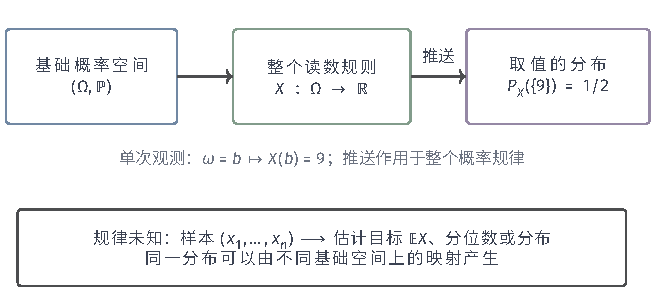
\includegraphics[width=\linewidth]{figures/02-mathematical-preliminaries-lower/01-random-variables-distributions-and-causality/tikz/rv-objects/figure.pdf}
  \caption{基础结果经随机变量映射成为读数；把事件概率推送到取值空间得到分布。分布未知时，样本用于估计指定目标，并不能唯一还原基础空间上的映射。}
\label{fig:rv-objects}
\end{figure}

\section{单个概率分布的描述}
\label{sec:rv-single-distribution}
前例中，不同设备状态可以得到同一个读数。若只关心读数，就把产生同一类读数的全部基础结果合在一起计算概率。设\(X\)取实值，它的分布测度记作\(\mathbb P_X\)，定义为
\[
 \mathbb P_X(B)=\mathbb P(X\in B)
 =\mathbb P\bigl(\{\omega:X(\omega)\in B\}\bigr),
 \qquad B\in\mathcal B(\mathbb R).
\]
这里\(B\)是读数空间中的集合，括号内的原像才是基础样本空间中的事件。\(\mathbb P\)给基础事件赋概率，\(\mathbb P_X\)给读数事件赋概率；等式说明二者怎样对应。随机变量\(X\)在取值空间上诱导的这个概率测度，称为它的\term{分布}（distribution）。

完整分布可以计算每个可测读数范围的概率。若当前只需要平均值或波动，可以先提取数值特征；若需要保留完整规律，则可用分布函数、相对于参考测度的密度，或积分变换来表示。为使后面的变换定义可直接使用，先建立期望。以下仍用\(F_X(x)=\mathbb P_X(({-\infty},x])\)表示累积到阈值\(x\)的概率，分布函数的性质在第~\ref{sec:rv-distribution}节说明。

\subsection{分布的数值特征}
\label{sec:rv-features}

完整分布能回答所有可测取值事件的概率，但一次计算往往只需要一个平均或波动尺度：报告一批读数的期望温度时，不必把整条分布列出来，只要一个数。数值特征通过对分布积分提取这些量。取值很大的地方可能只占很小的概率，所以定义平均之前，要核对相应的积分确实存在。
\label{sec:probability-expectation-conditional-expectation}
\paragraph{期望与均值}
% Baseline P:105-132
对非负随机变量\(X\)，定义
\[ \mathbb{E}[X]
  =\int_{\Omega}X(\omega)\,\mathrm{d}\mathbb{P}(\omega). \]
对一般实随机变量，写\(X=X^+-X^-\)。当
\(\mathbb{E}[|X|]<\infty\)时，正负两部分积分都有限，此时称\(X\)可积，并定义
\(\mathbb{E}[X]=\mathbb{E}[X^+]-\mathbb{E}[X^-]\)。不要求可积便随意相减\(\infty-\infty\)没有意义。

期望只依赖\(X\)的分布。对可测函数\(g\)，只要\(g(X)\)非负或可积，就有
\begin{equation}
  \mathbb{E}[g(X)]
  =
  \int_{\mathbb{R}}g(x)\,\mathrm{d}\mathbb{P}_X(x).
  \label{eq:probability-lotus}
\end{equation}
离散时，记\(p_X(x)=\mathbb P(X=x)\)，右侧是\(\sum_x g(x)p_X(x)\)；若分布具有密度\(f_X\)，即\(\mathbb P_X(B)=\int_B f_X(x)\,\mathrm dx\)，右侧则是\(\int g(x)f_X(x)\,\mathrm{d}x\)。这条“无须先求\(g(X)\)分布”的积分公式，会反复用于矩、蒙特卡洛估计和分布变换。

式~\eqref{eq:probability-lotus}直接来自推送测度的定义。对指示函数
\(g=\mathbb{I}_B\)，等式两侧分别为
\(\mathbb{P}(X\in B)\)与\(\mathbb{P}_X(B)\)，所以相等。线性性把结论推广到非负简单函数；任取递增到非负可测\(g\)的简单函数列，再在两侧使用单调收敛定理，即得非负情形。可积实值函数则分别对\(g^+\)和\(g^-\)应用这一结论。这个证明同时说明，等式并不要求\(X\)有密度。

\begin{example}[带噪观测的平均目标]
\label{ex:probability-noisy-observation}
设未知信号为\(\theta\)，观测为
\[ Y=\theta+\varepsilon,
  \qquad\mathbb{E}[\varepsilon]=0. \]
只要\(\varepsilon\)可积，就有\(\mathbb{E}[Y]=\theta\)。这并未说明一次读数接近
\(\theta\)，也未说明多个读数的平均必然收敛；后者还需要抽样依赖关系和矩条件。概率模型先把目标写成分布下的平均，后续误差结论再回答有限观测能否逼近这个平均。
\end{example}
\paragraph{方差与标准差}
% Baseline P:419-422
可积随机变量的均值记作\(\mu_X=\mathbb{E}[X]\)。若\(\mathbb{E}[X^2]<\infty\)，其方差为
\[ \operatorname{Var}(X)
  =\mathbb{E}\bigl[(X-\mu_X)^2\bigr]=\mathbb{E}[X^2]-\mu_X^2. \]
方差的非负平方根称为标准差，与原读数具有相同的计量单位。
% Baseline P:832-853

均值和方差便于计算，却不足以区分许多分布。若关心偏斜、尾部或独立和的分布变化，需要在这两个摘要之外保留信息：高阶矩增加摘要阶数；后面的积分变换还会把一系列摘要组织到一个函数中。

\paragraph{分位数}
% Baseline T:953-962
若给定累积概率水平\(q\in(0,1)\)，我们可以反过来寻找使累积概率达到或超过\(q\)的最小取值阈值。
\term{\(q\)分位数}（quantile）可定义为
\[
  F^{-1}(q)=\inf\{y:F(y)\geq q\},\qquad 0<q<1.
\]
这个广义逆为给定的\(F\)和\(q\)选出唯一的下分位数。更一般地，所有满足分位数
不等式的点组成集合
\[
  \mathcal Q_q=\{a:F(a^-)\leq q\leq F(a)\}.
\]
当\(F\)在水平\(q\)上存在平坦区间时，这个集合可能包含多个点；上述广义逆约定选取其中的下端代表。

\paragraph{高阶矩、偏度与峰度}
对正整数\(k\)，若\(\mathbb{E}[|X|^k]<\infty\)，则\(\mathbb{E}[X^k]\)称为\(k\)阶原点矩，
\(\mathbb{E}[(X-\mathbb{E}X)^k]\)称为\(k\)阶中心矩。三、四阶中心矩分别记录不对称性和大幅偏离均值的影响，但也随计量尺度改变。方差\(\sigma^2>0\)时，以\(\sigma^3\)和\(\sigma^4\)分别归一化，才得到偏度和峰度。有限低阶矩通常不能唯一确定分布。

\subsection{概率分布的表示}
\label{sec:rv-distribution}
数值特征只回答某一类查询。若要保留整个分布，可以记录全部阈值概率，也可以在参考测度下记录密度，或对一族指数函数积分。三种表示中的对象不同，存在条件也不同。

\subsubsection{基于分布函数的表示}
对实随机变量，分布函数为
\[ F_X(x)=\mathbb P_X(({-\infty},x])=\mathbb P(X\leq x). \]
它把一个概率测度写成一条关于阈值的函数。对\(a<b\)，半无限区间的差给出
\[ \mathbb P_X((a,b])=F_X(b)-F_X(a). \]
因此，知道全部\(F_X(x)\)就知道各半开区间的概率。由于这些区间生成实数轴的Borel事件族，分布函数唯一确定实数轴上的分布测度。

分布函数单调不减、右连续，且两端极限为
\[
  \lim_{x\to-\infty}F_X(x)=0,\qquad
  \lim_{x\to\infty}F_X(x)=1.
\]
反过来，每个具有这些性质的函数都对应某个实随机变量的分布。这是分布函数与分布测度之间的对应，不要求存在概率密度。

\subsubsection{基于参考测度的密度表示}
\label{sec:probability-radon-nikodym-change-measure}
若\(\mathbb{P}_X\)集中在可数点集上，可写成概率质量函数\(p_X(x)=\mathbb{P}(X=x)\)。若它相对于Lebesgue测度有密度\(f_X\)，则
\[ \mathbb{P}(X\in B)=\int_B f_X(x)\,\mathrm{d}x,
  \qquad F_X(x)=\int_{-\infty}^{x}f_X(t)\,\mathrm{d}t. \]
密度值不是单点概率。具有Lebesgue密度的分布满足\(\mathbb{P}(X=x)=0\)，但
\(f_X(x)\)仍可为正；在密度连续的点，它等于小邻域概率除以邻域长度后的局部极限；一般密度只在几乎处处意义下确定，不能在任意指定点都作这样的解释。
例如\(X\)在区间\([0,1/4]\)上均匀分布时，\(f_X(x)=4\mathbb{I}\{0\leq x\leq1/4\}\)。
密度值\(4\)可以大于\(1\)，因为概率由面积而非高度给出：
\(\mathbb{P}(0.10\leq X\leq0.15)=4\times0.05=0.2\)，而每个单点的概率仍为\(0\)。

图~\ref{fig:probability-density-cdf}把这一区分放在同一个分布上：密度图中的矩形面积，正是分布函数在区间两端的增量。因而从分布函数求区间概率不需要把连续结果变成单点概率。

\begin{figure*}[htbp]
  \centering
  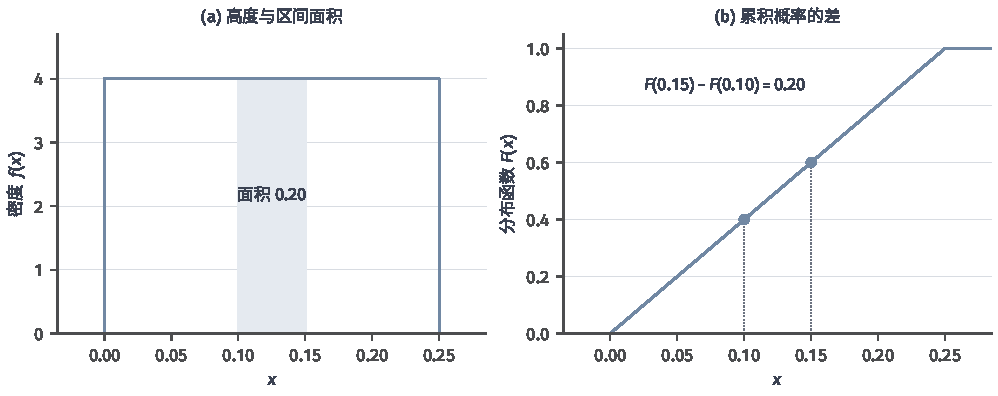
\includegraphics[width=\linewidth]{figures/02-mathematical-preliminaries-lower/01-random-variables-distributions-and-causality/matplotlib/probability-density-cdf/figure.pdf}
  \caption{区间\([0,1/4]\)上的均匀分布（解析式教学图）。左图阴影为\([0.10,0.15]\)的概率\(0.20\)，密度高度为\(4\)；右图的概率是\(F(0.15)-F(0.10)\)，两个端点本身均没有正概率质量。}
  \label{fig:probability-density-cdf}
\end{figure*}

在第~\ref{sec:probability-spaces-random-variables}节的四状态例子中，若把基础概率依次改成
\((0.1,0.2,0.3,0.4)\)，读数规则及取值范围都不变，但
\(\mathbb P(X=9)\)从\(1/2\)变成\(0.3\)。所以“能取哪些值”和“以什么概率取值”是两个问题。离散质量是相对于计数测度的密度；连续密度通常相对于Lebesgue测度，密度的数值不能脱离参考测度解释。
% Baseline P:136-246

离散的概率表与连续的密度函数，其实都是把分布写成某个参考测度下的权重：离散时参照计数测度，连续时通常参照Lebesgue测度。这引出一个统一的问题：在什么条件下，一个测度能写成另一个测度乘以某个权重，又怎样求出这个权重？
绝对连续先排除参考测度完全看不到的正质量区域，Radon--Nikodym导数在这一前提下给出权重；换测度时复用同一个权重，就不必为每种分布重新推导积分。

\paragraph{绝对连续与零集兼容性}
先考虑同一有限结果集合\(\Omega=\{\omega_1,\ldots,\omega_m\}\)上的两种概率分布\(P\)与\(Q\)。
记\(p_j=P(\{\omega_j\})\)、\(q_j=Q(\{\omega_j\})\)，则\((p_j)\)与\((q_j)\)就是两张概率表：各自列出每个结果出现的概率。
所谓“逐项比较”，就是固定同一个结果\(\omega_j\)，比较它在\(P\)下的概率\(p_j\)与在\(Q\)下的概率\(q_j\)。

例如，结果只有\(a,b,c\)三种，按这个顺序排列的概率表为
\[
  (p_1,p_2,p_3)=\left(\frac12,\frac14,\frac14\right),
  \qquad
  (q_1,q_2,q_3)=\left(\frac14,\frac14,\frac12\right).
\]
结果\(c\)在\(Q\)下出现的概率是在\(P\)下的两倍，\(a\)的概率则减半，\(b\)的概率不变。
若想用\(P\)下的样本估计\(Q\)下某个读数\(g\)的平均值，就应分别把\(a,b,c\)样本的读数乘以\(1/2,1,2\)，再对加权后的读数取样本平均。
这些权重正是\(q_j/p_j\)：在概率加权求和时，\(p_j\)乘以该比值就变成\(q_j\)，从而得到
\[
  \sum_{j=1}^{3}p_j\frac{q_j}{p_j}g(\omega_j)
  =\sum_{j=1}^{3}q_jg(\omega_j),
  \qquad (\omega_1,\omega_2,\omega_3)=(a,b,c).
\]
这里\(g\)是给每个结果指定一个实数读数的函数，右侧就是\(Q\)下的平均值。

上述例子中各个\(p_j\)均为正，概率比都有定义。但在一般的有限概率表中，若\(p_j=0\)而\(q_j>0\)，
\(P\)下的样本以概率\(1\)不会包含第\(j\)个结果，给已有样本重新加权也无法恢复\(Q\)分配给该结果的正概率。
例如，仍按\(a,b,c\)的顺序，改取
\[
  (p_1,p_2,p_3)=\left(\frac12,\frac12,0\right),
  \qquad
  (q_1,q_2,q_3)=\left(\frac14,\frac14,\frac12\right).
\]
从\(P\)抽样只能得到\(a\)和\(b\)，而\(Q\)给\(c\)分配了\(1/2\)的概率。
无论怎样调整\(a,b\)样本的权重，都不会产生\(c\)的贡献；即使给\(c\)指定任意有限权重\(w_c\)，其加权概率仍为
\[
  P(\{c\})w_c=0\times w_c=0,
\]
无法变成\(Q(\{c\})=1/2\)。所谓“无法补回这部分质量”，指的就是无法通过重加权恢复这\(1/2\)的概率。
若把读数取为\(g(\omega)=\mathbb{I}\{\omega=c\}\)，即只在结果为\(c\)时记为\(1\)、其余记为\(0\)，那么\(P\)样本的加权平均仍为\(0\)，而\(Q\)下的平均值为\(1/2\)。

图~\ref{fig:probability-zero-support-gap}把这一障碍画成两张概率表：\(a,b\)上的柱高可以经权重改变，\(c\)上为零的参考质量却没有可重加权的贡献。需要检查的是目标分布是否把正质量放在参考分布的零集上，而不是两组柱高是否接近。

\begin{figure}[htbp]
  \centering
  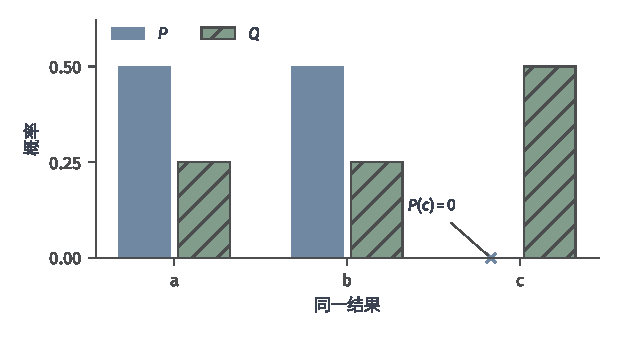
\includegraphics[width=105mm]{figures/02-mathematical-preliminaries-lower/01-random-variables-distributions-and-causality/matplotlib/probability-zero-support-gap/figure.pdf}
  \caption{参考分布缺少目标质量的三结果构造。蓝色实柱为\(P=(1/2,1/2,0)\)，绿色斜线柱为\(Q=(1/4,1/4,1/2)\)；叉号标出\(P(c)=0\)。任意有限权重仍给出\(P(c)w_c=0\)，不能恢复\(Q(c)=1/2\)。}
  \label{fig:probability-zero-support-gap}
\end{figure}

因此，若希望通过给\(P\)下的样本加权来计算\(Q\)下任意有界读数的平均，至少必须排除刚才的障碍：对每个结果\(\omega_j\)，只要\(P(\{\omega_j\})=0\)，就必须有\(Q(\{\omega_j\})=0\)。
这要求目标分布不给参考分布中概率为零的结果分配正概率。在有限结果集合上，检查所有单点就足够，因为任意事件的概率都是其中各个单点概率的和。

但在一般空间中，仅检查单点不够。例如，令\(P\)为\([0,1]\)上的均匀分布，\(Q\)为\([2,3]\)上的均匀分布。
两者对每个单点都给出零概率，却对事件\(A=[2,3]\)分别给出\(P(A)=0\)和\(Q(A)=1\)。
从\(P\)抽样无法得到落在\(A\)中的样本，给样本加权也无法恢复\(Q\)赋给\(A\)的概率。
所以，刚才的要求必须推广到每一个可测集合：
\[
  P(A)=0\Longrightarrow Q(A)=0,
  \qquad\text{对所有 }A\in\mathcal F\text{成立}.
\]
满足这一条件，就称\(Q\)对\(P\)绝对连续，记作\(Q\ll P\)。它把“参考分布中零概率的事件，在目标分布中也必须是零概率事件”写成了可检查的条件。

后面不仅要比较两个概率分布，还要讨论相对于计数测度、Lebesgue测度等参考测度的权重表示，因此把同一条件写成一般测度的定义。其中\(\mu\)对应参考测度，\(\nu\)对应希望表示的目标测度。
\begin{definition}[测度的绝对连续]
\label{def:probability-absolute-continuity}
设\(\nu\)与\(\mu\)为同一可测空间\((\Omega,\mathcal{F})\)上的测度。若
\[ \mu(A)=0\Longrightarrow\nu(A)=0,
  \qquad\text{对所有 }A\in\mathcal{F}\text{成立}, \]
则称\(\nu\)对\(\mu\)\term{绝对连续}（absolute continuity），记作\(\nu\ll\mu\)。
\end{definition}
它只要求\(\mu\)的零集也是\(\nu\)的零集，并不表示\(\nu(A)\leq\mu(A)\)，
也不自动提供有界的密度比。
这个定义先给出加权表示必须满足的零集条件，还没有构造权重函数。
接下来的有限分割计算先说明权重怎样由测度比得到；随后Radon--Nikodym定理再证明，在\(\sigma\)有限条件下，绝对连续足以保证一般空间中这样的权重函数存在。

\paragraph{有限分割上的密度表示}
先设\(\mu\)与\(\nu\)为有限测度，取有限可测分割
\(\Omega=A_1\mathbin{\dot\cup}\cdots\mathbin{\dot\cup}A_m\)，并假设\(\nu\ll\mu\)。
对\(\mu(A_j)>0\)的分块定义
\[ r(\omega)=\frac{\nu(A_j)}{\mu(A_j)},
  \qquad \omega\in A_j; \]
在\(\mu(A_j)=0\)的分块上令\(r=0\)。绝对连续性保证后一类分块也满足\(\nu(A_j)=0\)。因此，对任意由这些分块组成的事件\(A\)，
\[ \nu(A)=\int_A r\,\mathrm{d}\mu. \]
对在各分块上取有限实常数的函数\(g\)，逐项相加还给出
\begin{equation}
  \int_{\Omega}g\,\mathrm{d}\nu
  =
  \int_{\Omega}gr\,\mathrm{d}\mu.
  \label{eq:probability-finite-change-measure}
\end{equation}
一般定理要做的事，是在没有预先给定有限分块时构造同样的\(r\)\scite{math-kallenberg2021probability}。

\paragraph{一般测度的密度表示}
\begin{theorem}[Radon--Nikodym定理]
\label{thm:probability-radon-nikodym}
设\(\mu\)与\(\nu\)是\((\Omega,\mathcal{F})\)上的\(\sigma\)有限测度，且
\(\nu\ll\mu\)。则存在非负可测函数\(r\)，使每个\(A\in\mathcal{F}\)都满足
\begin{equation}
  \nu(A)=\int_A r\,\mathrm{d}\mu.
  \label{eq:probability-rn-representation}
\end{equation}
函数\(r\)在\(\mu\)-几乎处处意义下唯一，记为\(r=\mathrm{d}\nu/\mathrm{d}\mu\)，称为\term{Radon--Nikodym导数}
（Radon--Nikodym derivative）。
\end{theorem}

\begin{proof}
先设\(\mu,\nu\)有限，并令\(\lambda=\mu+\nu\)。在实线性空间
\(L^2(\lambda)\)上定义
\[
  T(f)=\int f\,\mathrm{d}\nu.
\]
由于\(\nu\leq\lambda\)，Cauchy--Schwarz不等式给出
\[
  |T(f)|
  \leq\int|f|\,\mathrm{d}\nu
  \leq\nu(\Omega)^{1/2}
       \left(\int f^2\,\mathrm{d}\nu\right)^{1/2}
  \leq\nu(\Omega)^{1/2}\lVert f\rVert_{L^2(\lambda)}.
\]
因此\(T\)是有界线性泛函。在完备内积空间中，有界线性泛函可以表示为与某个固定向量的内积。
\(L^2(\lambda)\)具有这一结构，所以存在
\(g\in L^2(\lambda)\)，使
\[
  \int f\,\mathrm{d}\nu=\int fg\,\mathrm{d}\lambda,
  \qquad f\in L^2(\lambda).
\]
这里用固定函数\(g\)表示测度\(\nu\)的积分，以便继续构造相对于\(\mu\)的密度；所用的Riesz表示性质可参考
\BookChapterRef{chap:functional-analysis-and-approximation}{卷1《数学准备：计算、分析与几何》的“函数空间”章}。
取\(f=\mathbb{I}_A\)可得\(\nu(A)=\int_Ag\,\mathrm{d}\lambda\)。若
\(A=\{g<0\}\)具有正测度，则对集合\(\{g\leq-1/k\}\)取指示函数会得到
\(\nu(\{g\leq-1/k\})<0\)的矛盾，故\(g\geq0\)几乎处处。又因为
\(\mu(A)=\lambda(A)-\nu(A)=\int_A(1-g)\,\mathrm{d}\lambda\geq0\)，同理有
\(g\leq1\)几乎处处。

令\(C=\{g=1\}\)。在\(C\)上有
\(\mu(C)=\int_C(1-g)\,\mathrm{d}\lambda=0\)，而\(\nu\ll\mu\)推出
\(\nu(C)=0\)。另一方面，\(\nu(C)=\int_Cg\,\mathrm{d}\lambda=\lambda(C)\)，所以
\(\lambda(C)=0\)。于是可以在其余部分定义
\[
  r=\frac{g}{1-g},
\]
并在\(C\)上任取值。由
\(\mathrm{d}\mu=(1-g)\,\mathrm{d}\lambda\)，对每个\(A\in\mathcal{F}\)都有
\[
  \int_A r\,\mathrm{d}\mu
  =\int_A\frac{g}{1-g}(1-g)\,\mathrm{d}\lambda
  =\int_Ag\,\mathrm{d}\lambda
  =\nu(A).
\]

若\(r_1,r_2\)都满足该表示，则对
\(A_k=\{r_1\geq r_2+1/k\}\)有
\[
  0=\int_{A_k}(r_1-r_2)\,\mathrm{d}\mu
  \geq\frac{1}{k}\mu(A_k),
\]
故\(\mu(A_k)=0\)。对\(k\)取并集得到\(r_1\leq r_2\)几乎处处；交换二者即得唯一性。

对\(\sigma\)有限的\(\mu,\nu\)，分别取有限测度覆盖并求交，可以把\(\Omega\)写成可数个互不相交、在两种测度下均有限的可测分块。在每个分块上使用上述构造，再把各块导数拼接，便得到全空间上的\(r\)。拼接后的表示可先对有限个分块验证，再由单调收敛推广到全部分块。
\end{proof}

这个证明先让\(\lambda=\mu+\nu\)同时支配两种测度，再把测度\(\nu\)表示为
\(L^2(\lambda)\)中的函数\(g\)。绝对连续性只用于排除\(g=1\)承载正质量，保证比值
\(g/(1-g)\)能够成为相对于\(\mu\)的密度。构造得到的是可测密度，并没有得到逐点上界。

\subsubsection{基于积分变换的表示}
\label{sec:probability-moment-transforms}
\paragraph{矩母函数与累积量生成函数}
逐个列出高阶矩，不便处理独立累计量。指数函数有一个方便的性质：它的幂级数把各阶幂放进同一个表达式；在允许交换求导与期望时，对参数求导便能取回相应的矩。对独立变量，和的指数矩又分解为各自指数矩的乘积，取对数就把这种乘积变成加法，因此同一构造还适合研究累计和。定义中的有限邻域用于保证这些运算有可用的起点。
\begin{definition}[矩母函数与累积量生成函数]
  \label{def:probability-moment-generating-functions}
设\(X\)为实随机变量。若存在\(\delta>0\)，使\(\mathbb E e^{tX}<\infty\)对全部\(|t|<\delta\)成立，则在该邻域上定义\term{矩母函数}（moment-generating function, MGF）为
\[ M_X(t)=\mathbb{E}[e^{tX}]. \]
\term{累积量生成函数}（cumulant-generating function）是
\[ K_X(t)=\log M_X(t). \]
\end{definition}
若可在积分号下求导，则\(M_X^{(k)}(0)=\mathbb{E}[X^k]\)。
矩存在却不保证矩母函数在原点邻域有限。取密度为
\(e^{-z^2/2}/\sqrt{2\pi}\)的标准高斯变量\(Z\)，令\(X=e^Z\)；
这样得到的正随机变量称为对数正态变量（lognormal random variable）。
对每个正整数\(k\)，配方得到
\[
 \mathbb E X^k
 =\frac1{\sqrt{2\pi}}\int_{\mathbb R}e^{kz-z^2/2}\,\mathrm dz
 =e^{k^2/2}<\infty.
\]
但对任意\(t>0\)，指数矩的被积函数是
\(e^{te^z-z^2/2}/\sqrt{2\pi}\)。当\(z\to+\infty\)时，\(e^z\)的增长压过\(z^2\)，
该被积函数最终大于\(1\)，所以在正半轴上的积分发散。
因此\(\mathbb E e^{tX}=\infty\)，虽有全部正整数阶矩，仍不满足上述邻域条件。

矩母函数满足上述有限邻域条件时，累积量生成函数的前两阶导数分别给出均值和方差。对随机向量\(\bm{X}\)，若联合指数矩在零向量的某个开邻域内有限，则定义
\[ K_{\bm{X}}(\bm{t})
  =\log\mathbb{E}\bigl[e^{\bm{t}^{\top}\bm{X}}\bigr], \]
混合偏导数给出联合累积量。独立变量的变换函数乘积及累积量可加法则在第~\ref{sec:rv-combinations}节说明。

% Baseline P:856-870
前两阶关系可以直接核对。若存在\(\delta>0\)，使
\(\mathbb E e^{tX}<\infty\)对全部\(|t|<\delta\)成立，取\(0<\delta_1<\delta_2<\delta\)。对\(|t|\leq\delta_1\)及\(j=1,2\)，存在有限常数\(C_j\)，使
\[ |X|^j e^{tX}\leq C_j\bigl(e^{\delta_2X}+e^{-\delta_2X}\bigr). \]
右侧可积，且不随\(t\)变化，因而允许在积分下求导，得到
\[
  M_X'(t)=\mathbb{E}[Xe^{tX}],\qquad
  M_X''(t)=\mathbb{E}[X^2e^{tX}].
\]
因为\(M_X(0)=1\)，
\[
  K_X'(0)=\frac{M_X'(0)}{M_X(0)}=\mathbb{E}X,
  \qquad
  K_X''(0)
  =M_X''(0)-M_X'(0)^2
  =\operatorname{Var}(X).
\]
矩母函数可能在零点的任何双侧邻域都不有限。研究分布极限时，需要一个对所有实参数都存在的变换。
\paragraph{特征函数与分布唯一性}
% Baseline P:875-878
\begin{definition}[特征函数]
  \label{def:probability-characteristic-function}
实随机变量\(X\)的特征函数为\(\varphi_X(t)=\mathbb E e^{\mathrm i tX}\)，其中\(t\in\mathbb R\)。随机向量的版本为\(\varphi_{\bm X}(\bm t)=\mathbb E e^{\mathrm i\bm t^\top\bm X}\)。复数期望分别对实部与虚部积分。
\end{definition}
由于复指数的绝对值恒为\(1\)，特征函数总存在。它用振荡而非指数放大取值，因此与可能发散的矩母函数承担不同职责；后面将用它把独立和的分布极限转成函数的逐点极限。

变换还有一个有限低阶矩所没有的性质：保留完整的特征函数，就保留了分布。
\begin{theorem}[变换函数的分布唯一性]
\label{thm:rv-transform-uniqueness}
同维随机向量的特征函数在所有实向量参数上相同，当且仅当它们的分布相同。
若两个矩母函数都在原点的某个共同开邻域内有限，并在该邻域内相同，
它们也确定相同的分布。
\end{theorem}
这里引用概率变换的唯一性定理，不展开所需的Fourier反演论证\scite{math-kallenberg2021probability}。
它把“两个变换相同”转成“两个分布相同”；只比较有限个矩或有限个参数点，
没有这种唯一性保证。

\section{随机变量的联合、条件与独立关系}
\label{sec:rv-relations}
两台设备即使各自具有相同误差分布，共同偏高与一高一低仍会给出不同的平均结果。下面先建立联合规律和独立性，再说明已知一项读数后怎样更新另一项的描述。

\subsection{随机变量的联合关系}
\label{sec:rv-joint}
\label{sec:probability-joint-marginal-conditional}
\subsubsection{联合分布与边缘分布}
% Baseline P:312-333
随机向量\((X,Y)\)的联合分布是映射\(\omega\mapsto(X(\omega),Y(\omega))\)在乘积空间上诱导的概率测度。离散情形中，
联合质量\(p_{X,Y}(x,y)\)给出完整表格，边缘分布由求和消去另一坐标：
\[ p_X(x)=\sum_y p_{X,Y}(x,y),
  \qquad p_Y(y)=\sum_x p_{X,Y}(x,y). \]
若联合分布有密度，则相应运算变为
\[ f_X(x)=\int f_{X,Y}(x,y)\,\mathrm{d}y. \]
一般情形不需要质量函数或密度。记坐标投影为\(\pi_X(x,y)=x\)，则边缘分布就是联合分布经\(\pi_X\)的推送：
\[
  \mathbb{P}_X(A)
  =\mathbb{P}_{(X,Y)}(A\times\mathcal{Y}).
\]
对非负可测函数\(g\)，式~\eqref{eq:probability-lotus}给出
\[
  \int g(x)\,\mathbb{P}_X(\mathrm{d}x)
  =
  \int g\bigl(\pi_X(x,y)\bigr)\,
       \mathbb{P}_{(X,Y)}(\mathrm{d}x,\mathrm{d}y).
\]
若联合分布有密度，再对右侧使用Tonelli定理，才得到对\(y\)积分的边缘密度公式。因而“边缘化”首先是测度推送，求和或积分只是它在特定参考测度下的表达。

边缘化会丢掉变量如何共同变化的信息。两个不同联合分布可以拥有完全相同的两个边缘分布：只看各自边缘，看不出两个读数是一起升高、彼此独立还是总朝相反方向变化。下面用一个只取两个值的例子把这一丢失演示出来。

\subsubsection{协方差与相关系数}
% Baseline P:423-430
已知两个边缘方差，还不能判断合成读数的波动。将各读数减去自身均值后再相乘，就可把同向偏离与反向偏离区分开；把这些乘积按联合规律平均，得到进入和的方差公式的交叉项。这个量只保留二阶共同变化，不能代替完整联合分布。
对二阶可积的\(X,Y\)，协方差为
\[ \operatorname{Cov}(X,Y)
  =\mathbb{E}\bigl[(X-\mathbb{E}X)(Y-\mathbb{E}Y)\bigr]. \]
Cauchy--Schwarz不等式保证它有限。方差满足
\[ \operatorname{Var}(aX+b)=a^2\operatorname{Var}(X), \]
而
\[ \operatorname{Var}(X+Y)
  =\operatorname{Var}(X)+\operatorname{Var}(Y)+2\operatorname{Cov}(X,Y). \]
只有协方差为零时，方差才直接相加；独立是协方差为零的充分条件，但通常不是必要条件。

若各坐标二阶可积，随机向量的均值和协方差为
% Baseline P:1090-1098
\[ \bm{\mu}=\mathbb{E}\bm{X},
  \qquad\bm{\Sigma}=\mathbb{E}\bigl[(\bm{X}-\bm{\mu})(\bm{X}-\bm{\mu})^{\top}\bigr]. \]
对任意\(\bm{u}\in\mathbb{R}^d\)，
\[
  \bm{u}^{\top}\bm{\Sigma}\bm{u}
  =\mathbb{E}\left[
    \bigl(\bm{u}^{\top}(\bm{X}-\bm{\mu})\bigr)^2
  \right]\geq0,
\]
所以协方差矩阵总是对称半正定。

若两个变量的方差都为正，相关系数定义为
\[ \rho_{X,Y}=\frac{\operatorname{Cov}(X,Y)}{\sqrt{\operatorname{Var}(X)\operatorname{Var}(Y)}}. \]
Cauchy--Schwarz不等式给出\(|\rho_{X,Y}|\leq1\)。零方差变量是几乎处处常数，不应代入分母为零的相关系数公式。
把读数转换成二元误差标记\(U,V\in\{0,1\}\)。令两个标记各自以概率\(1/2\)取零或一，即固定边缘规律为
\[
U\sim\operatorname{Bernoulli}(1/2),\qquad
V\sim\operatorname{Bernoulli}(1/2).
\]
图~\ref{fig:rv-dependence}中的联合质量仍可给出三种不同的平均效果：
\[
\begin{array}{c|ccc}
 & V=U & U,V\text{独立} & V=1-U\\ \hline
\operatorname{Cov}(U,V)&1/4&0&-1/4\\
\mathbb P(U+V=0)&1/2&1/4&0\\
\mathbb P(U+V=1)&0&1/2&1\\
\mathbb P(U+V=2)&1/2&1/4&0
\end{array}
\]
\begin{figure}[htbp]
  \centering
  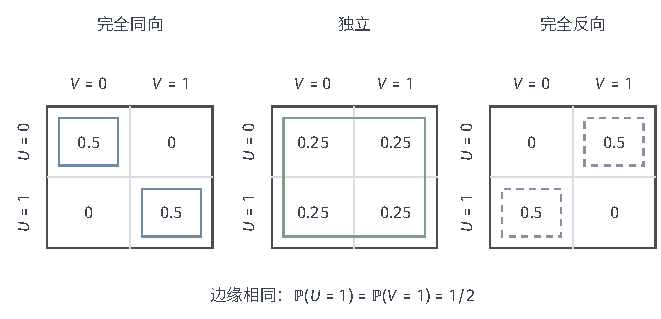
\includegraphics[width=\linewidth]{figures/02-mathematical-preliminaries-lower/01-random-variables-distributions-and-causality/tikz/rv-dependence/figure.pdf}
  \caption{边缘质量相同的三个联合分布。格内数字是联合概率，各行各列的和始终为\(1/2\)；质量的位置改变协方差及和的分布。}
\label{fig:rv-dependence}
\end{figure}

\begin{example}[区域分布的质心与主轴]
\label{ex:probability-region-moments}
设平面区域\(A\subset\mathbb R^2\)的面积\(|A|\)有限且非零，并有有限二阶矩。在\(A\)上按面积均匀抽取位置\(\bm X=(X_1,X_2)^\top\)，其均值与协方差为
\[
 \bm\mu=\frac1{|A|}\int_A\bm x\,\mathrm d\bm x,
 \qquad
 \bm\Sigma=\frac1{|A|}\int_A(\bm x-\bm\mu)(\bm x-\bm\mu)^\top\,\mathrm d\bm x.
\]
均值是区域的质心；单位方向\(\bm u\)上的位置方差为\(\bm u^\top\bm\Sigma\bm u\)。因此最大特征值的特征向量给出位置分散最大的主轴方向；最大特征值重复时，这个方向可能不唯一。图像区域的面积、质心与二阶矩可用同一分布语言表示，但这里均匀抽取的是位置，不是把像素灰度直接当作概率。
\end{example}

\subsection{随机变量的独立关系}
\label{sec:probability-moments-independence}
% Baseline P:720-821

联合规律可能由边缘规律直接相乘得到。此时，知道一项取什么值不会改变另一项的分布；这种关系称为独立性。先用事件概率描述它，再检查它与零协方差的区别。

\subsubsection{独立、不相关与非线性依赖}
若随机变量\(X,Y\)满足
\[ \mathbb{P}(X\in A,Y\in B)
  =\mathbb{P}(X\in A)\mathbb{P}(Y\in B) \]
对所有Borel集合\(A,B\)成立，就称二者\term{独立}（independent）。对非负可测函数\(g,h\)，独立性给出
\[
 \mathbb{E}[g(X)h(Y)]=\mathbb{E}[g(X)]\mathbb{E}[h(Y)],
\]
等式按非负扩展实数解释，并约定\(0\cdot\infty=0\)。对实值函数，若\(g(X)\)与\(h(Y)\)分别可积，则乘积也可积，且同一等式两侧均为有限值。
证明从指示函数开始：独立性正好说明结论对
\(g=\mathbb{I}_A\)、\(h=\mathbb{I}_B\)成立。线性性把它推广到非负简单函数，再分别对两个因子使用单调收敛，得到非负情形。
对分别可积的实值因子，先把非负结论用于\(|g|,|h|\)，得到乘积的绝对期望有限，再分解正负部分即可。
仅有乘积可积并不足够：一个因子恒为零时乘积可积，另一个因子的期望却可能不存在，不能据此写出右侧的有限期望乘积。

协方差只检查中心化变量的一次乘积。令\(X\)在\([-1,1]\)上均匀分布，并取\(Y=X^2\)。对称性给出
\[ \operatorname{Cov}(X,Y)
  =\mathbb{E}[X^3]-\mathbb{E}[X]\mathbb{E}[X^2]=0, \]
但\(Y\)由\(X\)完全决定；知道\(X\)便能确定\(Y\)，所以二者不独立。零协方差只排除了线性二阶关联。

\subsection{随机变量的条件关系}
看到第一台设备的读数后，第二台设备原来的边缘描述可能不再充分。若查询的是平均读数，可以把已见信息固定下来计算条件期望；若查询的是越界概率、分位数或下一次随机生成的规律，则需要条件分布。两项查询使用相同的信息，但要求保留的结果不同。

\subsubsection{条件信息下的均值关系}
\label{sec:rv-conditional-expectation}
% Baseline P:434-524
预测一个结果时，可用的信息往往不是结果本身，而只是一部分观察：可能知道一次测量落在哪个区间却不知道精确数值，也可能知道掷出的点数是奇数却不知道是几点。要把“知道一部分”写成可以计算的对象，需要先说清哪些事件能由这部分信息区分，再要求预测在每个可区分的事件上保持原有的平均。

有限情形可以直接说清。若手头的信息只把样本空间分成有限组\(A_1,\ldots,A_m\)，那么预测值在每组之内只能取同一个常数——超过了这些信息就没有依据；而要让这个常数不与已知信息冲突，取该组内\(X\)的平均是自然的选择。于是“只用已有信息”与“不改变各组平均”这两条要求，共同确定了预测值。表~\ref{tab:probability-finite-partition-predictions}给出可以逐项核对的例子。

连续取值时不能照搬“给定\(X=x\)”这一步。若\(P(X=x)=0\)，事件\(\{X=x\}\)的概率为零，比值
\(\mathbb E[X\mathbb I_{\{X=x\}}]/\mathbb P(X=x)\)成为\(0/0\)，没有定义；对每个\(x\)都零概率地单独处理，也无法拼出一个整体的答案。这正是需要换一种写法的原因。

出路是放弃逐点条件，改为整体要求：答案在每一个仅由\(X\)决定的事件上保持原来的平均。仅由\(X\)决定的事件正是\(\sigma(X)\)中的集合，因而条件用子\(\sigma\)代数表示，而不是用单个事件表示。下面先明确“由观察生成的信息”，再给出这一定义。

子\(\sigma\)代数\(\mathcal{G}\subseteq\mathcal{F}\)表示当前可用信息。预测值只能使用这些信息，并且在每个可以由当前信息区分的事件上保持原来的平均。
\begin{definition}[观测生成的信息]
  \label{def:probability-generated-information}
若\(X:\Omega\to(\mathcal X,\mathcal A)\)是随机变量，记
\(\sigma(X)=\{X^{-1}(A):A\in\mathcal A\}\)。它是使\(X\)可测的最小\(\sigma\)代数，表示仅观察\(X\)能够区分的事件。多个观测生成的信息是包含它们全部可测逆像的最小\(\sigma\)代数。
\end{definition}
例如只观察分组编号，就不能在同一组内区分两个原始结果。写\(\mathbb E[Y\mid X]\)时，真正限制答案的信息是\(\sigma(X)\)，不是单个零概率事件\(\{X=x\}\)。
\begin{definition}[条件期望]
  \label{def:probability-conditional-expectation}
对\(X\in L^1(\mathbb P)\)，\term{条件期望}（conditional expectation）
\(\mathbb{E}[X\mid\mathcal{G}]\)是满足下列两项条件的可积随机变量\(Z\)：
\[ Z\text{ 对 }\mathcal{G}\text{ 可测},
  \qquad\int_A Z\,\mathrm{d}\mathbb{P}=\int_A X\,\mathrm{d}\mathbb{P}\quad(A\in\mathcal{G}). \]
\end{definition}
第一项要求答案只能使用\(\mathcal{G}\)中的信息，第二项要求它在每个可由当前信息识别的事件上保留\(X\)的平均\scite{math-kallenberg2021probability}。在有限分组情形，第二项正是“每组内部平均值不变”，第一项正是“同组之内取同一个常数”；两条合起来就唯一确定了前面所说的逐组平均。

这里有一点容易忽略：条件期望本身是一个随机变量，不是常数。\(\mathbb E[X\mid\mathcal G]\)随\(\omega\)变化，但它只通过\(\mathcal G\)能够区分的部分变化——在同一组之内取值相同。所以它是“把已知信息作为输入的函数”，写成\(\mathbb E[X\mid X]\)等于\(X\)，写成\(\mathbb E[X\mid \{\varnothing,\Omega\}]\)则是常数\(\mathbb E X\)。已知的信息越多，\(\mathcal G\)越大，答案就越细致；两个极端分别是不用任何信息和已知全部信息。

\begin{theorem}[条件期望的存在与唯一性]
\label{thm:probability-conditional-expectation-existence}
若\(X\in L^1(\mathbb{P})\)，则\(\mathbb{E}[X\mid\mathcal{G}]\)存在，并在几乎处处意义下唯一。
\end{theorem}

\begin{proof}
先设\(X\geq0\)。在\((\Omega,\mathcal{G})\)上定义有限测度
\[ \nu(A)=\int_A X\,\mathrm{d}\mathbb{P}. \]
若\(\mathbb{P}(A)=0\)，则\(\nu(A)=0\)，所以\(\nu\ll\mathbb{P}|_{\mathcal{G}}\)。Radon--Nikodym定理给出非负、
\(\mathcal{G}\)-可测的\(Z\)，使\(\nu(A)=\int_A Z\,\mathrm{d}\mathbb{P}\)。对一般可积\(X\)，分别对
\(X^+\)与\(X^-\)使用这一构造并取差，即得存在性。

若\(Z_1,Z_2\)都满足定义，令\(D=Z_1-Z_2\)。对每个\(A\in\mathcal{G}\)，\(\int_A D\,\mathrm{d}\mathbb{P}=0\)。若
\(\mathbb{P}(D>0)>0\)，则某个集合\(A_k=\{D\geq1/k\}\)具有正概率，从而
\[ \int_{A_k}D\,\mathrm{d}\mathbb{P}
  \geq\frac{1}{k}\mathbb{P}(A_k)>0, \]
产生矛盾。因此\(D\leq0\)几乎处处。交换\(Z_1,Z_2\)可得\(D\geq0\)几乎处处，故二者几乎处处相等。
\end{proof}

积分的线性性与上述唯一性说明，条件期望也保持线性组合。
对非负变量，存在证明给出的Radon--Nikodym导数非负；
因此若\(X\leq Y\)且两者可积，对\(Y-X\)使用该构造便得到
\(\mathbb E[X\mid\mathcal G]\leq\mathbb E[Y\mid\mathcal G]\)几乎处处。
这就是条件期望的保序性。

若\(X\)本来就对\(\mathcal{G}\)可测，则\(\mathbb{E}[X\mid\mathcal{G}]=X\)几乎处处。若\(X\)与\(\mathcal{G}\)
独立，则条件期望等于常数\(\mathbb{E}[X]\)。若\(U\)有界且\(\mathcal{G}\)-可测，则
\begin{equation}
  \mathbb{E}[UX\mid\mathcal{G}]
  =
  U\mathbb{E}[X\mid\mathcal{G}].
  \label{eq:probability-taking-out-known-factor}
\end{equation}
可积的非有界\(U\)需要另外核对乘积可积性，不能仅凭“已知量可提出”略去条件。

有限分组把抽象定义化成逐组平均。若
\(A_1,\ldots,A_m\)是有限可测分割，
\(\mathcal{G}=\sigma(A_1,\ldots,A_m)\)，且每个
\(\mathbb{P}(A_j)>0\)，则
\begin{equation}
  \mathbb{E}[X\mid\mathcal{G}]
  =
  \sum_{j=1}^{m}
  \frac{\mathbb{E}[X\mathbb{I}_{A_j}]}
       {\mathbb{P}(A_j)}
  \mathbb{I}_{A_j}.
  \label{eq:probability-finite-partition-conditional-expectation}
\end{equation}
若某个分组概率为零，该组上的取值可以任意指定，因为条件期望只在几乎处处意义下唯一。

表~\ref{tab:probability-finite-partition-predictions}给出一个可复核例子。令
\(\mathcal{G}\)只能区分
\(A=\{\omega_1,\omega_2\}\)与
\(B=\{\omega_3,\omega_4\}\)。不使用分组信息时，最佳常数预测是
\(U_0=\mathbb{E}X=3.4\)；规则\(U_{\mathrm{grp}}\)虽然按组取值，却随意地在
\(A,B\)上分别预测\(0,4\)；条件均值\(m=\mathbb{E}[X\mid\mathcal{G}]\)则在两组
上分别等于\(1.2,5.6\)。
\begin{table}[htbp]
  \centering
  \small
  \begin{tabular}{ccccccc}
    \toprule
    结果 & 概率 & \(X\) & 分组 & \(U_0\) & \(U_{\mathrm{grp}}\) & \(m\) \\
    \midrule
    \(\omega_1\) & \(0.2\) & \(0\) & \(A\) & \(3.4\) & \(0\) & \(1.2\) \\
    \(\omega_2\) & \(0.3\) & \(2\) & \(A\) & \(3.4\) & \(0\) & \(1.2\) \\
    \(\omega_3\) & \(0.1\) & \(4\) & \(B\) & \(3.4\) & \(4\) & \(5.6\) \\
    \(\omega_4\) & \(0.4\) & \(6\) & \(B\) & \(3.4\) & \(4\) & \(5.6\) \\
    \midrule
    \multicolumn{4}{r}{平方风险\(\ \mathbb{E}[(X-U)^2]\)} &
    \(5.64\) & \(2.80\) & \(0.80\) \\
    \bottomrule
  \end{tabular}
  \caption{有限分组下的三类预测。分组信息使预测可以随\(A,B\)变化，但只有逐组条件
  均值在全部\(\mathcal{G}\)-可测平方可积预测中达到最小平方风险。}
  \label{tab:probability-finite-partition-predictions}
\end{table}
按定义核对\(m\)，只需在\(\mathcal{G}\)能区分的事件上验证第二条要求，即
\(A,B,\varnothing,\Omega\)。在\(A\)上，
\[
  \int_A X\,\mathrm{d}\mathbb{P}
  =0\times0.2+2\times0.3=0.6
  =\mathbb{P}(A)\times1.2
  =\int_A 1.2\,\mathrm{d}\mathbb{P},
\]
在\(B\)上同理有\(4\times0.1+6\times0.4=2.8=0.5\times5.6\)。而在\(\Omega\)上两者
都等于\(\mathbb E X=3.4\)，这正是全期望公式在两组情形下的表现。反过来，
\(U_{\mathrm{grp}}\)在\(A\)上取值\(0\)而组内平均为\(1.2\)，第二条要求不满足，
所以它不是条件期望。逐组平均之所以在这里唯一确定答案，是因为除两个分组外
\(\mathcal{G}\)不再含其他集合，核对任务只有这么几项；一般情形下可测性要求把范围
限制在\(\sigma(A_1,\ldots,A_m)\)中，结论仍然相同。

三列风险依次说明不同问题：获得分组信息可以优于无信息常数，但使用信息本身不保证已经
最优；式~\eqref{eq:probability-finite-partition-conditional-expectation}还要在每组
内选择正确的条件平均。三列中只有\(m\)同时满足两条定义条件，风险\(0.80\)也比另外两列低，
这两个事实不是巧合：\(\mathcal{G}\)-可测平方可积预测中使平方风险最小者，正是条件期望，
下面的平方分解会说明原因。
% Baseline P:532-625
\begin{theorem}[塔式性质]
\label{thm:probability-tower-property}
若\(X\in L^1\)，且\(\mathcal{H}\subseteq\mathcal{G}\subseteq\mathcal{F}\)，则
\[ \mathbb{E}\bigl[\mathbb{E}[X\mid\mathcal{G}]
  \mid\mathcal{H}\bigr]=\mathbb{E}[X\mid\mathcal{H}] \]
几乎处处成立。
\end{theorem}

\begin{proof}
左侧对\(\mathcal{H}\)可测。对任意\(A\in\mathcal{H}\)，由于\(A\in\mathcal{G}\)，条件期望定义给出
\[
  \int_A
  \mathbb{E}\bigl[\mathbb{E}[X\mid\mathcal{G}]
  \mid\mathcal{H}\bigr]\,\mathrm{d}\mathbb{P}
  =
  \int_A\mathbb{E}[X\mid\mathcal{G}]\,\mathrm{d}\mathbb{P}
  =
  \int_A X\,\mathrm{d}\mathbb{P}.
\]
左侧因而满足\(X\)关于\(\mathcal{H}\)的条件期望定义，唯一性给出结论。
\end{proof}

取\(\mathcal{H}=\{\varnothing,\Omega\}\)，便得到\term{全期望公式}（law of total expectation）
\begin{equation}
  \mathbb{E}\bigl[\mathbb{E}[X\mid\mathcal{G}]\bigr]
  =
  \mathbb{E}[X].
  \label{eq:probability-total-expectation}
\end{equation}
这说明条件化改变可用信息，却不改变再平均后的总体均值。

\paragraph{全方差分解}
设\(X\in L^2\)，记\(m=\mathbb{E}[X\mid\mathcal{G}]\)。分解
\[ X-\mathbb{E}X=(X-m)+(m-\mathbb{E}X). \]
在展开平方前，需要先确认条件均值仍然二阶可积。
对每个有理数\(q\)，条件期望的线性性与保序性给出
\[
 \mathbb E[X^2\mid\mathcal G]-2qm+q^2
 =\mathbb E[(X-q)^2\mid\mathcal G]\geq0.
\]
有理数只有可数个，可以在同一个满测集上同时使用这些不等式。
由于\(\sup_{q\in\mathbb Q}(2qm-q^2)=m^2\)，得到
\[
  |m|^2
  \leq
  \mathbb{E}[X^2\mid\mathcal{G}].
\]
再取期望并使用全期望公式，得到
\[
  \mathbb{E}[m^2]\leq\mathbb{E}[X^2]<\infty.
\]
因此\(m\in L^2\)，上面分解中的两项都二阶可积，其乘积由Cauchy--Schwarz不等式保证可积。又因为第二项对
\(\mathcal{G}\)可测，而\(\mathbb{E}[X-m\mid\mathcal{G}]=0\)，所以交叉项期望为
\[ \mathbb{E}\bigl[(X-m)(m-\mathbb{E}X)\bigr]
  =\mathbb{E}\left[(m-\mathbb{E}X)\mathbb{E}[X-m\mid\mathcal{G}]\right]=0. \]
展开平方得到\term{全方差公式}（law of total variance）
\begin{equation}
  \operatorname{Var}(X)
  =
  \mathbb{E}\bigl[\operatorname{Var}(X\mid\mathcal{G})\bigr]
  +
  \operatorname{Var}\bigl(\mathbb{E}[X\mid\mathcal{G}]\bigr),
  \label{eq:probability-total-variance}
\end{equation}
其中
\[ \operatorname{Var}(X\mid\mathcal{G})
  =\mathbb{E}\bigl[(X-m)^2\mid\mathcal{G}\bigr]. \]
第一项是获得\(\mathcal{G}\)后仍无法解释的平均波动，第二项是不同信息状态之间的可解释波动。

刚才的平方界是条件Jensen不等式（conditional Jensen inequality）的一个实例。
一般地，若\(\phi:\mathbb R\to\mathbb R\)为凸函数，\(X\)与\(\phi(X)\)都可积，则
\[
 \phi\bigl(\mathbb E[X\mid\mathcal G]\bigr)
 \leq\mathbb E[\phi(X)\mid\mathcal G]\quad\text{几乎处处}.
\]
其依据仍是仿射下界：在每个有理点选取一条支撑线
\(a_qx+b_q\leq\phi(x)\)，凸函数的连续性保证这些支撑线的上确界等于\(\phi\)。
对每条线取条件期望，得到
\(a_qm+b_q\leq\mathbb E[\phi(X)\mid\mathcal G]\)，
再在共同满测集上取可数上确界即可。
对有限维随机向量，把支撑线换成仿射支撑超平面，论证相同；
凸函数只定义在凸域上时，还需条件均值属于该域，并核对相关量的可积性。
取不含额外信息的平凡条件，便得到通常的积分Jensen不等式。

\paragraph{条件均值的平方损失最优性}
\begin{theorem}[条件均值的平方损失最优性]
\label{thm:probability-conditional-mean-l2-projection}
设\(X\in L^2(\mathbb{P})\)。在所有\(\mathcal{G}\)-可测且二阶可积的随机变量\(U\)中，
\[ m=\mathbb{E}[X\mid\mathcal{G}] \]
唯一地在几乎处处意义下最小化\(\mathbb{E}[(X-U)^2]\)。
\end{theorem}

\begin{proof}
\(L^2(\mathcal{G})\)是\(L^2(\mathcal{F})\)的闭线性子空间，上文直接证明的条件平方界已经说明
\(m\in L^2(\mathcal{G})\)。对每个\(U\in L^2(\mathcal{G})\)，Cauchy--Schwarz不等式保证
\((X-m)U\)可积，因而可以提出已知因子并使用塔式性质，得到
\[ \mathbb{E}[(X-m)U]
  =\mathbb{E}\left[U\mathbb{E}[X-m\mid\mathcal{G}]\right]=0. \]
所以\(X-m\)与整个\(L^2(\mathcal{G})\)正交，\(m\)就是\(X\)到该闭子空间的正交投影。直接展开
\begin{equation}
  \mathbb{E}[(X-U)^2]
  =
  \mathbb{E}[(X-m)^2]
  +
  \mathbb{E}[(m-U)^2],
  \label{eq:probability-pythagorean-prediction}
\end{equation}
交叉项因正交性消失。第二项非负，且仅当\(U=m\)几乎处处时为零。
\end{proof}

图~\ref{fig:probability-conditional-projection}把这一平方分解放在一个能画出的精确模型中。设基础结果只有两种，概率各为\(1/2\)，且可用信息不能区分它们。每个随机变量由它在两种结果上的取值表示为一个平面向量；允许的预测只能是常量，因此落在对角线\(U=(c,c)\)上。取\(X=(0,2)\)，其条件均值为\(m=(1,1)\)。若改用\(U=(2,2)\)，则\(X-m\)与\(m-U\)正交，平方风险从最小值\(1\)增加为\(1+1=2\)。这里的距离来自随机变量之间的\(L^2\)范数，图中的两个坐标不是两次抽样的时间顺序。一般条件信息可对应更高维的可测预测子空间，同一个正交分解仍由上面的证明给出。

\begin{figure}[htbp]
  \centering
  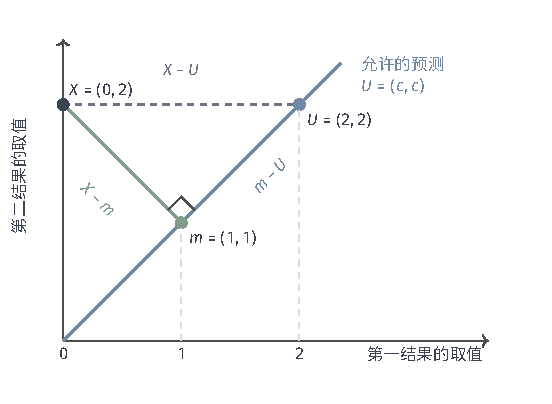
\includegraphics[width=92mm]{figures/02-mathematical-preliminaries-lower/01-random-variables-distributions-and-causality/tikz/probability-conditional-projection/source.pdf}
  \caption{两等概率结果上的条件均值投影。横纵坐标分别记录随机变量在两个基础结果上的取值；平凡信息下允许预测的集合是对角线。\(m\)是\(X\)在该线上的投影，直角标记对应误差正交。此例的\(L^2\)范数平方是图中欧氏长度平方的\(1/2\)，所以三边对应的平方风险满足\(2=1+1\)。}
  \label{fig:probability-conditional-projection}
\end{figure}

条件期望的存在只需要\(X\in L^1\)，这时它由Radon--Nikodym导数给出。“正交投影”和平方损失最优性则需要\(X\in L^2\)。若二阶矩无限，条件期望仍可能
存在，但不能直接套用上述\(L^2\)投影结论。

\subsubsection{条件信息下的分布关系}
\label{sec:rv-conditional-distribution}
% Baseline P:370-413
当条件变量连续时，事件\(\{X=x\}\)常有零概率，直接相除不再可行。需要把“每个条件值对应一个分布”组织成能继续积分的对象。
\begin{definition}[概率核]
  \label{def:probability-kernel}
  给定可测空间\((\mathcal X,\mathcal A)\)、\((\mathcal Y,\mathcal B)\)，\term{概率核}（probability kernel）是映射
  \[ K:\mathcal X\times\mathcal B\to[0,1], \]
  满足：对每个\(x\in\mathcal X\)，\(K(x,\cdot)\)是\((\mathcal Y,\mathcal B)\)上的概率测度；对每个\(B\in\mathcal B\)，\(x\mapsto K(x,B)\)是\(\mathcal A\)-可测函数。
\end{definition}
第一项保证每个条件值给出合法分布，
第二项保证再对\(X\)积分是合法运算。

可测并不等于连续。例如取在\([-1,1]\)上均匀分布的\(X\)，令\(Y=\mathbb I\{X\geq0\}\)，则\(K(x,\{1\})=\mathbb I\{x\geq0\}\)是合法概率核在事件\(\{1\}\)上的取值，却在\(x=0\)处跳变。条件值\(x\)可以连续取值，条件分布随\(x\)变化仍可不连续。

\begin{definition}[正则条件分布]
  \label{def:probability-regular-conditional-distribution}
若概率核\(K\)对所有\(A\in\mathcal A\)、\(B\in\mathcal B\)满足
\begin{equation}
  \mathbb{P}(X\in A,Y\in B)
  =
  \int_A K(x,B)\,\mathbb{P}_X(\mathrm{d}x),
  \label{eq:probability-regular-conditional-kernel}
\end{equation}
就把\(K(x,\cdot)\)称为\(Y\)给定\(X=x\)的一个\term{正则条件分布}（regular conditional distribution）。
\end{definition}
对每个固定可测集\(B\)，两个版本的\(K(x,B)\)在\(\mathbb P_X\)-几乎处处意义下相同；若\(\mathcal Y\)是下面的标准Borel空间，还可选取一个共同零测集，使其外的条件概率测度相同。零概率条件点上的取值通常不能由联合分布唯一决定。

\begin{example}[条件分布版本可以怎样不同]
\label{ex:probability-conditional-kernel-versions}
设\(X\sim\operatorname{Unif}[0,1]\)，并令\(Y=X\)。给定\(x\)，取
\(K(x,\cdot)=\delta_x\)，即全部条件概率质量集中在\(y=x\)。对任意Borel集\(A,B\)，
\[
 \begin{aligned}
 \mathbb P(X\in A,Y\in B)
 &=\mathbb P(X\in A\cap B)\\
 &=\int_A\mathbb I_B(x)\,\mathbb P_X(\mathrm dx)
  =\int_A K(x,B)\,\mathbb P_X(\mathrm dx).
 \end{aligned}
\]
因此\(K\)是一个正则条件分布。现在只在\(x=1/2\)处把\(\delta_x\)改成\(\delta_0\)，
其余点不变，得到另一个可测概率核\(\widetilde K\)。由于
\(\mathbb P_X(\{1/2\})=0\)，上述积分不变，\(\widetilde K\)也是同一联合分布的条件版本。
两个版本在共同零测集\(\{1/2\}\)之外给出完全相同的概率测度。

这里每个单点\(\{x\}\)都有零概率，却不能因此在所有点上任意改值：不可数个零概率
单点的并集可以具有正概率。若把全部\(K(x,\cdot)\)都改成\(\delta_0\)，它就不再
重建\(Y=X\)的联合分布。“几乎处处唯一”约束的是两个完整条件核可以在哪一整个
集合上不同，而不是逐点检查后随意拼接答案。

此例的联合分布全部集中在对角线\(y=x\)上。对角线的二维Lebesgue测度为零，
所以不存在普通二维联合密度；正则条件分布仍然存在。条件核因而比密度比值公式更一般。
\end{example}

\paragraph{正则条件分布的存在条件}
逐个条件事件的概率能够定义，并不保证它们能拼成一个共同的概率核。下面的可测空间条件为这种拼接提供保证。
\begin{definition}[Polish空间]
  \label{def:probability-polish-space}
从一个度量空间出发，允许更换距离但保持同一族开集。
若能选到完备且可分的距离，就称这个空间为Polish空间。
保持开集不变也保持相同的连续映射，这就是“距离与原拓扑兼容”的含义。
可分表示含有可数稠密子集；完备性表示所选距离下每个Cauchy序列都在空间内收敛。
\end{definition}
欧氏空间就是一个例子。这里要求存在合适的距离，不要求最初写下的那个距离已经完备。
例如\((0,1)\)的通常距离不完备，但连续双射\(x\mapsto\log(x/(1-x))\)
把它映到实轴，逆也连续；拉回实轴距离得到
\[
 d'(x,y)=\left|\log\frac{x}{1-x}-\log\frac{y}{1-y}\right|.
\]
这个距离保持原开集，并把该区间变为与实轴等距的完备可分空间。
标准Borel空间进一步只保留这样的可测结构。
\begin{definition}[标准Borel空间]
  \label{def:probability-standard-borel-space}
  可测空间称为\term{标准Borel空间}（standard Borel space），若它与某个完备可分度量空间的Borel子集可测同构，即存在双射，且该双射及其逆映射都可测。
\end{definition}
这里不要求展示出来的Borel子集在继承距离下完备。
若\(X\)与\(Y\)的状态空间都是标准Borel空间，则上述正则条件分布存在。实数空间、欧氏空间、可数集合以及配备适当Borel结构的常见可分函数空间都属于这一范围。

这一存在结论依赖可数生成结构与上一小节的条件期望：需要把逐个事件上的条件平均整理成同一个概率核。

在完全一般的可测空间上，正则条件分布可能不存在。此时条件期望仍可相对于子\(\sigma\)代数定义，但不能未经说明就把它写成每个点\(x\)上的条件密度。后续模型
通常工作在标准Borel空间中；使用\(p(y\mid x)\)时，应同时确认密度所依赖的参考测度及其适用的几乎处处范围。

% Baseline P:526-528
实值\(Y\)的构造可以用有理阈值说明。对每个\(q\in\mathbb Q\)，先取条件期望
\[
 Z_q=\mathbb E[\mathbb I\{Y\leq q\}\mid\sigma(X)].
\]
它是基础空间上的随机变量；要构造条件核，还要把它写成观测值\(x\)的函数。
选取取值于\([0,1]\)的条件期望版本。可测因子分解给出Borel可测函数\(H_q\)，使\(Z_q=H_q(X)\)；必要时将\(H_q\)截到\([0,1]\)，不改变这个等式。
这一步可由简单函数逼近看出：每个\(\sigma(X)\)中的事件都是某个可测集在\(X\)下的原像，
所以\(\sigma(X)\)-可测简单函数能写成\(X\)的函数；对非负可测变量递增逼近并取极限，便得到所需分解。
因此这里先得到\(H_q(X)\)这个条件期望版本，再把\(H_q(x)\)组织成分布，尚未用零概率事件相除。
有理数可数，因而能去掉同一个\(\mathbb P_X\)-零测集，使\(H_q\)同时满足单调性、
\(H_q=\inf_{r>q,\ r\in\mathbb Q}H_r\)，以及\(H_{-m}\to0\)、\(H_m\to1\)。
这些关系分别来自条件期望的单调性和条件单调收敛；右侧的下确界可用预先选定的有理递减序列计算。
在余下的\(x\)上令
\[ F_x(y)=\inf_{q>y,\ q\in\mathbb Q}H_q(x). \]
它是分布函数，故唯一确定一个实数轴上的概率测度。对半无限区间，事件概率关于\(x\)可测；
半无限区间生成实数轴的Borel集；可测性和条件概率恒等式又在相应的单调极限下保留，所以单调类论证可把二者推广到全部Borel事件。共同零测集上统一选择一个点质量，就得到完整概率核。
一般标准Borel取值空间可借助与实数轴Borel子集的可测同构完成同样构造，再把测度映回原空间。
在该子集上的全质量条件也只需排除一个共同零测集。完整的分解定理见\scite{math-kallenberg2021probability}。
% Baseline P:335-366
当\(p_X(x)>0\)时，离散条件质量定义为
\[ p_{Y\mid X}(y\mid x)
  =\frac{p_{X,Y}(x,y)}{p_X(x)}. \]
因此有乘法公式
\[ p_{X,Y}(x,y)=p_X(x)p_{Y\mid X}(y\mid x). \]
若\(p_Y(y)>0\)，把联合质量按另一顺序分解便得到Bayes公式
\begin{equation}
  p_{X\mid Y}(x\mid y)
  =
  \frac{p_{Y\mid X}(y\mid x)p_X(x)}
       {\sum_{x'}p_{Y\mid X}(y\mid x')p_X(x')}.
  \label{eq:probability-discrete-bayes}
\end{equation}
分母是观测\(y\)的边缘概率，既负责归一化，也要求观测并非零概率事件。

连续密度公式是同一分解的特例。若\((X,Y)\)相对于两个\(\sigma\)有限参考测度的乘积有联合密度
\(f_{X,Y}\)，且\(0<f_X(x)<\infty\)，则
\[
  f_{Y\mid X}(y\mid x)
  =\frac{f_{X,Y}(x,y)}{f_X(x)}
\]
非负并对\(y\)积分为\(1\)。它满足
\(f_{X,Y}(x,y)=f_X(x)f_{Y\mid X}(y\mid x)\)。在
\(f_X(x)=0\)或\(f_X(x)=\infty\)的点上，不能使用这个比值；这些点构成\(\mathbb P_X\)-零测集。条件核在该零测集上可统一指定一个固定概率测度，而不改变联合分布。这里选用由联合密度积分得到的边缘密度版本；任意修改过的密度版本也只能保证相应等式几乎处处成立。

\begin{example}[有限候选经过带噪观测更新]
\label{ex:probability-finite-candidate-bayes}
设信号只可能是\(\Theta\in\{-1,1\}\)，先验概率均为\(1/2\)。传感器以概率\(0.8\)报告正确符号。观测\(Y=1\)后，
\[ \mathbb{P}(\Theta=1\mid Y=1)
  =\frac{0.8\times0.5}{0.8\times0.5+0.2\times0.5}=0.8. \]
观测并未把候选集合改成一个确定点，而是改变了两个候选的相对权重。若某个观测在所有
候选下概率都为零，公式分母为零，条件分布不能靠这个比值定义。
\end{example}
% Baseline T:970-975
先不区分条件变量\(X\)的取值、只看读数\(Y\)，得到的是\(Y\)的边缘分布及其分位数。若\(Y\)在不同\(X=x\)下具有不同的位置或尾部，边缘分位数一般不能代替给定\(X=x\)时的条件分位数。例如，温度读数在不同负载下可能具有不同的上分位数，把负载混合后得到的阈值未必适用于每个负载层。若\(X\)与\(Y\)独立，条件分布则可取为同一个边缘分布，相应分位数相同。这里的\(X\)表示用于条件化的变量，不预先限定为预测器的输入特征。
\begin{definition}[条件分位数]
  \label{def:statistics-conditional-quantile}
给定\(Y\)关于\(X=x\)的正则条件分布，记\(F_x(y)=\mathbb P(Y\leq y\mid X=x)\)。对\(0<q<1\)，下条件\(q\)分位数为\(F_x^{-1}(q)=\inf\{y:F_x(y)\geq q\}\)；完整条件分位数集合为\(\{a:F_x(a^-)\leq q\leq F_x(a)\}\)。这些对象随条件分布版本确定，并按\(P_X\)-几乎处处意义理解。
\end{definition}
条件分位数是已知条件分布的特征；从联合观测样本估计整条条件分位函数的方法见第~\ref{sec:statistics-nonparametric-missing}节。

\subsubsection{条件独立及其运算规则}
两台传感器可能因共享环境温度而相关；固定温度以后，剩余噪声却可能彼此独立。此时“没有额外信息”的比较应在同一个背景值内进行，而不是比较混合不同温度后的边缘分布。条件独立将这个分层要求写成条件概率的乘积分解。
\begin{definition}[条件独立]
  \label{def:probability-conditional-independence}
  给定随机变量\(X,Y,Z\)，若对\(X,Y\)取值空间中的所有可测集合\(A,B\)，
\[ \mathbb{P}(X\in A,Y\in B\mid Z)
  =\mathbb{P}(X\in A\mid Z)\mathbb{P}(Y\in B\mid Z) \]
几乎处处成立，就称\(X\)与\(Y\)在给定\(Z\)时条件独立，记作
\(X\perp Y\mid Z\)。
\end{definition}
它表示\(Z\)已知以后，\(X\)不再提供关于\(Y\)的额外分布信息；这不意味着去掉\(Z\)后仍独立。

两个方向的差别都可以用掷两次硬币说清。设\(X,Y\)为两次独立投掷的结果，\(Z=X\oplus Y\)为
二者的异或（相同取\(0\)，不同取\(1\)）。无条件下\(X\)与\(Y\)独立；但已知\(Z\)后，
\(X\)的取值完全决定\(Y\)，条件独立不成立。反向的例子是取\(Z\)为一次公平投掷的结果，
并令\(X=Y=Z\)：无条件时\(X\)与\(Y\)完全相关，而给定\(Z\)后两者都成为确定值，
条件独立成立。这说明\(X\perp Y\mid Z\)与\(X\perp Y\)之间没有单向的推出关系，
必须分别说明是哪个命题。

条件独立满足以下常用规则：
\[
\begin{aligned}
  X\perp Y\mid Z
  &\Longrightarrow Y\perp X\mid Z
  &&\text{（对称性）},\\
  X\perp(Y,W)\mid Z
  &\Longrightarrow X\perp Y\mid Z
  &&\text{（分解）},\\
  X\perp(Y,W)\mid Z
  &\Longrightarrow X\perp Y\mid Z,W
  &&\text{（弱并）},\\
  X\perp Y\mid Z,\quad X\perp W\mid Y,Z
  &\Longrightarrow X\perp(Y,W)\mid Z
  &&\text{（收缩）}.
\end{aligned}
\]
在所涉状态空间为标准Borel空间的情形，下面可以用条件核的乘积分解验证这些规则。交性质
\[ X\perp Y\mid Z,W,\quad
  X\perp W\mid Z,Y\Longrightarrow X\perp(Y,W)\mid Z \]
并非无条件成立；严格为正的有限离散联合质量是一个常用充分条件。若分布把质量集中在
低维约束上，零概率组合会阻断所需的消元步骤。

\begin{lemma}[严格正离散分布的交性质]
  \label{lem:probability-positive-intersection}
  设$I$为有限索引集，每个$i\in I$对应取值于有限非空状态空间$\mathcal{X}_i$的随机变量$X_i$。令$p$为$\bm{X}=(X_i)_{i\in I}$在乘积状态空间$\mathcal{X}=\prod_{i\in I}\mathcal{X}_i$上的联合质量函数，且$p(\bm{x})>0$对所有$\bm{x}\in\mathcal{X}$成立。对两两不交的索引集$A,B,C,D\subseteq I$，若
  \[
    \bm{X}_A\perp\bm{X}_B\mid(\bm{X}_C,\bm{X}_D),
    \qquad
    \bm{X}_A\perp\bm{X}_D\mid(\bm{X}_C,\bm{X}_B),
  \]
  则
  \[
    \bm{X}_A\perp(\bm{X}_B,\bm{X}_D)\mid\bm{X}_C.
  \]
\end{lemma}

\begin{proof}
严格正性保证以下每个条件概率都有定义。对任意取值$\bm{a},\bm{b},\bm{c},\bm{d}$，两个前提分别给出
\[
  p(\bm{a}\mid\bm{b},\bm{c},\bm{d})
  =p(\bm{a}\mid\bm{c},\bm{d}),
  \qquad
  p(\bm{a}\mid\bm{b},\bm{c},\bm{d})
  =p(\bm{a}\mid\bm{b},\bm{c}).
\]
因此$p(\bm{a}\mid\bm{c},\bm{d})=p(\bm{a}\mid\bm{b},\bm{c})$对每个$\bm{b},\bm{d}$成立。固定任意基准值$\bm{b}^{\circ}$，右侧等于$q(\bm{a},\bm{c})=p(\bm{a}\mid\bm{b}^{\circ},\bm{c})$，不再依赖$\bm{b}$或$\bm{d}$。对$(\bm{b},\bm{d})$关于$p(\bm{b},\bm{d}\mid\bm{c})$求和可得$q(\bm{a},\bm{c})=p(\bm{a}\mid\bm{c})$，故$p(\bm{a}\mid\bm{b},\bm{c},\bm{d})=p(\bm{a}\mid\bm{c})$，这正是所需的条件独立性。
\end{proof}
严格正性使上面证明能在固定\(\bm c\)后独立改变\(\bm b\)和\(\bm d\)。若只支持部分组合，这一步会失败。一个反例是\(X=Y=W=B\)，其中\(B\)为非退化Bernoulli变量，\(Z\)取常数。给定\(W\)后\(X,Y\)都确定，所以\(X\perp Y\mid W\)；给定\(Y\)后也有\(X\perp W\mid Y\)。但\(X\)与\((Y,W)\)显然不独立，因为后者直接给出\(X\)。两个条件独立前提因而不能在这类带零概率配置的分布上推出交性质。

以分解和收缩为例可以看清这些规则使用了什么。若
\(X\perp(Y,W)\mid Z\)，则对任意可测集合\(A,B,C\)，条件核满足
\[
  K_{X,Y,W\mid Z}(A,B,C\mid z)
  =K_{X\mid Z}(A\mid z)K_{Y,W\mid Z}(B,C\mid z).
\]
令\(C\)取全集便得到
\(K_{X,Y\mid Z}=K_{X\mid Z}K_{Y\mid Z}\)，这就是分解规则。对收缩规则，假设
\[
  K_{X,Y\mid Z}=K_{X\mid Z}K_{Y\mid Z},
  \qquad
  K_{X,W\mid Y,Z}=K_{X\mid Y,Z}K_{W\mid Y,Z}.
\]
第一个条件还给出
\(K_{X\mid Y,Z}=K_{X\mid Z}\)的一个版本。沿条件乘法公式相乘可得
\[
  K_{X,Y,W\mid Z}
  =K_{X\mid Z}K_{Y\mid Z}K_{W\mid Y,Z}
  =K_{X\mid Z}K_{Y,W\mid Z},
\]
即\(X\perp(Y,W)\mid Z\)。所有等式都按相应条件变量分布的几乎处处意义理解。概率图模型部分会在这些概率规则之上另加图分离语义；图上没有边本身并不是这里定义的条件独立证明。

\section{常见概率分布}
\label{sec:probability-common-distributions}
\label{sec:probability-families-transformations}
一次试验的成功标记只能取零或一，固定次数中的成功数取整数，等待时间和随机比例则分别有非负与区间取值限制。分布模型要先满足这些取值要求，再说明各个概率由什么假设决定。例如事件数取非负整数，只限定了支持；要采用Poisson规律，还需支持相应的到达假设。下面按取值空间介绍常用分布，并同时说明决定分布形状的假设。

\subsection{离散取值下的概率分布}
\paragraph{Bernoulli分布}
% Baseline P:885-902
把一次试验的成功记为\(1\)、失败记为\(0\)，只需一个成功概率便能确定整张概率表。
\term{Bernoulli分布}以参数\(p\in[0,1]\)描述一次二元结果：
\[ \mathbb{P}(X=x)=p^x(1-p)^{1-x},
  \qquad x\in\{0,1\}, \]
且\(\mathbb{E}X=p\)、\(\operatorname{Var}(X)=p(1-p)\)。

\paragraph{二项分布}
设每次成功概率为\(p\)，共作\(n\)次独立的同类试验。若只保留成功总数，就要把所有具有相同成功次数的排列概率相加：固定\(k\)次成功时，每个排列的概率为\(p^k(1-p)^{n-k}\)，共有\(\binom nk\)种排列。这个计数给出下面的质量函数。
\(n\)个独立同分布的
Bernoulli变量之和服从\term{二项分布}
\[ \mathbb{P}(S=k)
  =\binom{n}{k}p^k(1-p)^{n-k},\qquad k=0,\ldots,n, \]
其均值和方差分别为\(np\)与\(np(1-p)\)。这里及后续离散质量公式约定零次幂为\(1\)，包含\(0^0=1\)；这样参数端点也给出相应的点质量。

\paragraph{类别分布}
给定\(K\)个类别以及概率向量\(\bm p\)，其中\(p_k\geq0\)且\(\sum_kp_k=1\)。类别变量\(C\in\{1,\ldots,K\}\)满足
\(\mathbb P(C=k)=p_k\)，称为类别分布。类别编号只是标记，编号的均值通常没有物理含义；用独热向量
\(\bm e_C\)表示时，其均值就是概率向量\(\bm p\)。多项分布描述多次独立类别抽取后的整组计数。

\paragraph{多项分布}
若一次试验有\(K\)个类别，概率向量\(\bm{p}\)满足\(p_k\geq0\)及\(\sum_kp_k=1\)。\(n\)次独立试验的类别计数\(\bm{N}\)服从\term{多项分布}，质量为
\[ \mathbb{P}(\bm{N}=\bm{n})
  =\frac{n!}{\prod_{k=1}^{K}n_k!}\prod_{k=1}^{K}p_k^{n_k},\qquad\sum_{k=1}^{K}n_k=n. \]
各类计数之和固定为\(n\)，一个类别多计一次，其他类别就少一次。为记录这种共同变化，协方差取两个计数各自减去均值后的乘积再求平均：同向偏离贡献为正，反向偏离贡献为负。下面的负交叉项对应不同类别竞争固定总次数；第~\ref{sec:rv-joint}节已给出相应的一般公式。
其均值为\(\mathbb{E}N_k=np_k\)，协方差为\(\operatorname{Cov}(N_j,N_k)=n(p_j\mathbb{I}\{j=k\}-p_jp_k)\)。

\paragraph{Poisson分布}
固定试验次数适合描述二项计数，但一个时间窗口里的到达次数通常没有预设上限。一个典型模型来自大量独立的小机会：若机会数增加、每次成功概率减小，而平均成功数趋向\(\lambda\)，二项质量趋向下面的形式。它说明Poisson模型的一种来源；仅知道事件数非负，仍不足以断定采用这个模型。
\term{Poisson分布}以\(\lambda>0\)描述固定窗口中的事件计数：
\[ \mathbb{P}(N=k)
  =e^{-\lambda}\frac{\lambda^k}{k!},\qquad k=0,1,\ldots, \]
且均值、方差都为\(\lambda\)。独立计数的相加规律在第~\ref{sec:rv-combinations}节推导。

Poisson计数没有固定的最大次数；二项计数的上界则是已知试验次数\(n\)。二者不能只按均值接近就视为同一个模型。

\subsection{连续取值下的概率分布}
\paragraph{均匀分布}
固定有限区间\([a,b]\)，其中\(a<b\)。若等长的子区间具有相同概率，就得到连续均匀分布（uniform distribution）\(X\sim\operatorname{Unif}[a,b]\)，密度为
\[ f_X(x)=\frac{1}{b-a}\mathbb I_{[a,b]}(x). \]
直接积分给出\(\mathbb E X=(a+b)/2\)、\(\operatorname{Var}(X)=(b-a)^2/12\)。它规定区间内概率按长度分配；“不知道结果”本身不足以推出均匀假设。

\paragraph{指数分布}
% Baseline P:908-913
计数问一个窗口内发生了几次，等待时间则问下一次事件何时发生。若已经等待多久不改变接下来继续等待的规律，可用下面的指数模型表达这种假设；它适合恒定到达强度下的等待，而不是任意非负时长。
\term{指数分布}以速率\(\lambda>0\)描述等待时间，密度为
\[
f_T(t)=\lambda e^{-\lambda t}\mathbb I_{\{t\geq0\}}.
\]
其均值为\(1/\lambda\)、方差为\(1/\lambda^2\)，并对\(s,t\geq0\)满足无记忆性：
\[ \mathbb{P}(T>s+t\mid T>s)=\mathbb{P}(T>t). \]
无记忆性只适用于已经等待的时长不改变剩余等待分布，不表示不同等待时间自动独立。
它与Poisson事件计数的联系在第~\ref{sec:rv-poisson}节给出过程定义后建立。

无记忆性可以逐项验算，从而看出它为什么是特殊性质而非普遍规律。取\(\lambda=1\)，
已知\(T>s\)的概率为\(e^{-s}\)，于是
\[
  \mathbb{P}(T>s+t\mid T>s)
  =\frac{\mathbb{P}(T>s+t)}{\mathbb{P}(T>s)}
  =\frac{e^{-(s+t)}}{e^{-s}}=e^{-t}
  =\mathbb{P}(T>t),
\]
与\(s\)无关。这一化简依赖于指数函数的除法把\(s\)消去，其他分布一般做不到：
设\(T\)在\([0,1]\)上均匀分布，则在\(T>0.5\)的条件下，剩余等待不超过\(0.2\)的概率是
\(0.2/0.5=0.4\)，而无条件下同一概率只有\(0.2\)。已经等了半程这件事本身携带信息，
说明该分布没有无记忆性。反过来看，无记忆性也刻画了指数分布：在非负、非退化且生存概率连续并始终为正的等待时间模型中，满足这一等式的分布必为某个正速率的指数分布。

这一性质决定了指数分布适合描述什么。元件若已使用\(s\)小时，其剩余寿命分布与全新元件
相同，就适用指数模型；若磨损会使剩余寿命变短，则不适用。同一句话也说清了它与独立的
区别：无记忆性谈论同一个变量在条件前后的分布，与两个变量之间是否独立是两回事。
% Baseline P:927-1014

\paragraph{高斯分布}
等待时间只能非负，温度等有符号读数却可以在中心值两侧波动。一个常用的对称模型以中心位置和波动尺度确定密度，离中心越远密度越低；下面的高斯模型就是这种选择。多个独立小误差累计为何会近似产生这一形状，将在中心极限定理中另加条件说明，不能只由对称性推出。
\term{高斯分布}（Gaussian distribution，也称正态分布）
\(X\sim\mathcal{N}(\mu,\sigma^2)\)具有密度
\[ f_X(x)
  =\frac{1}{\sqrt{2\pi\sigma^2}}\exp\left\{-\frac{(x-\mu)^2}{2\sigma^2}\right\},\qquad \sigma^2>0. \]
其均值为\(\mu\)，方差为\(\sigma^2\)。当\(a\neq0\)时，仿射变换满足\(aX+b\sim\mathcal{N}(a\mu+b,a^2\sigma^2)\)；当\(a=0\)时，结果是集中于\(b\)的点质量，可记作退化高斯，但不能再使用上面的正方差密度。

\paragraph{Gamma分布}
正变量上的密度常含有\(x^{a-1}e^{-bx}\)这一形状。要把它归一化，需要一个依赖形状参数的积分常数。
\begin{definition}[Gamma函数]
  \label{def:probability-gamma-function}
对实数\(a>0\)，定义Gamma函数为
\begin{equation}
  \Gamma(a)=\int_0^\infty t^{a-1}e^{-t}\,\mathrm dt,
  \qquad a>0.
  \label{eq:probability-gamma-function}
\end{equation}
\end{definition}
\(a>0\)保证零附近的幂函数可积，指数衰减保证无穷远处可积。
分部积分给出\(\Gamma(a+1)=a\Gamma(a)\)，并且\(\Gamma(1)=1\)，所以对正整数
\(n\)，有\(\Gamma(n)=(n-1)!\)。它把阶乘延伸到这里需要的正实参数，对\(b>0\)，换元
\(t=bx\)说明\(\int_0^\infty x^{a-1}e^{-bx}\,\mathrm dx=\Gamma(a)/b^a\)。

形状参数\(a>0\)、速率参数\(b>0\)的\term{Gamma分布}密度为
\[ f_X(x)
  =\frac{b^a}{\Gamma(a)}x^{a-1}e^{-bx}\mathbb{I}\{x>0\}. \]
其均值为\(a/b\)，方差为\(a/b^2\)。指数分布是\(a=1\)的特例。若使用尺度参数
\(\vartheta=1/b\)，公式会改变；引用Gamma分布时必须说明采用速率还是尺度参数。

\paragraph{Beta分布}
若\(U\sim\operatorname{Gamma}(a,1)\)与\(V\sim\operatorname{Gamma}(b,1)\)独立，则
\[ R=\frac{U}{U+V} \]
服从\term{Beta分布}\(\operatorname{Beta}(a,b)\)。为得到归一化常数，令
\(S=U+V\)，于是\(U=RS\)、\(V=(1-R)S\)，变换的Jacobian绝对值为\(s\)。独立Gamma密度经过换元得到
\[
  f_{R,S}(r,s)
  =
  \frac{r^{a-1}(1-r)^{b-1}}{\Gamma(a)\Gamma(b)}
  s^{a+b-1}e^{-s},
  \qquad 0<r<1,\ s>0.
\]
对\(s\)积分并使用Gamma函数定义，得到
\[
  f_R(r)
  =
  \frac{\Gamma(a+b)}{\Gamma(a)\Gamma(b)}
  r^{a-1}(1-r)^{b-1}\mathbb{I}\{0<r<1\}.
\]
因此
\[
  \mathbb{E}R=\frac{a}{a+b},\qquad
  \operatorname{Var}(R)=
  \frac{ab}{(a+b)^2(a+b+1)}.
\]
Beta分布适合描述\([0,1]\)上的随机比例。
这里共同速率使比例与总量分离；两个Gamma变量速率不同则不能直接得到该Beta结论。

\paragraph{Dirichlet分布}
当\(K\geq2\)、每个\(\alpha_k>0\)时，独立变量\(G_k\sim\operatorname{Gamma}(\alpha_k,1)\)的归一化比例
\[ P_k=\frac{G_k}{\sum_{j=1}^{K}G_j} \]
服从下面定义的Dirichlet分布。其均值为
\(\mathbb{E}P_k=\alpha_k/\alpha_0\)，其中\(\alpha_0=\sum_k\alpha_k\)。同样令
\(S=\sum_kG_k\)，把前\(K-1\)个比例和总量作为新坐标；Jacobian为
\(s^{K-1}\)。联合密度分成一个形状为\(\alpha_0\)的Gamma密度和一个比例密度。这给出：
\begin{definition}[Dirichlet分布]
  \label{def:probability-dirichlet-distribution}
设\(K\geq2\)、\(\alpha_k>0\)且\(\alpha_0=\sum_k\alpha_k\)。随机向量\(\bm P\)取值于概率单纯形，若以前\(K-1\)个坐标为自由坐标、令\(p_K=1-\sum_{k<K}p_k\)，相对于\(\mathrm dp_1\cdots\mathrm dp_{K-1}\)的密度为
\[
  f_{\bm{P}}(\bm{p})
  =
  \frac{\Gamma(\alpha_0)}
       {\prod_{k=1}^{K}\Gamma(\alpha_k)}
  \prod_{k=1}^{K}p_k^{\alpha_k-1},
  \qquad p_k>0,\quad\sum_kp_k=1,
\]
并在上述自由坐标域以外取零，就称其服从\term{Dirichlet分布}，记作\(\operatorname{Dirichlet}(\alpha_1,\ldots,\alpha_K)\)。\(K=1\)时约定为\(P_1=1\)的点质量。
\end{definition}
这不是相对于\(K\)维Lebesgue测度的密度：单纯形在该测度下为零集。选定自由坐标，也就明确了归一化常数所对应的参考测度。
由Beta边缘或直接积分可得
\[
  \operatorname{Var}(P_k)
  =\frac{\alpha_k(\alpha_0-\alpha_k)}
        {\alpha_0^2(\alpha_0+1)},\qquad
  \operatorname{Cov}(P_j,P_k)
  =-\frac{\alpha_j\alpha_k}
         {\alpha_0^2(\alpha_0+1)}
  \quad(j\neq k).
\]
负协方差来自各坐标之和固定为\(1\)。例如
\(\operatorname{Beta}(8,2)\)的均值为\(0.8\)、方差为
\(16/1100\approx0.0145\)；\(\operatorname{Beta}(80,20)\)均值仍为\(0.8\)，方差降为
\(1600/1010000\approx0.00158\)。参数总量增大使质量更集中，却不表示已经观察到相同比例的真实频数；参数如何由观测到的类别计数更新属于第~\ref{sec:rv-inference}节的统计推断问题。Beta分布是\(K=2\)时对一个坐标的描述。

\paragraph{多元高斯分布}
对无约束向量，常用均值为\(\bm\mu\)、协方差为\(\bm\Sigma\)的高斯模型。
% Baseline P:1108-1112
第~\ref{sec:rv-joint}节的协方差矩阵记录所有线性组合的方差，却没有确定这些组合的完整分布。若进一步要求任意加权合成的读数仍为高斯，就把一维高斯规律扩展到整个向量；只要求每个坐标各自高斯还不能控制坐标之间的联合关系。
\begin{definition}[多元高斯随机向量]
  \label{def:probability-multivariate-gaussian}
  若对每个\(\bm{u}\in\mathbb{R}^d\)，标量
\(\bm{u}^{\top}\bm{X}\)都服从一维高斯分布，就称\(\bm{X}\)为\term{多元高斯随机向量}（multivariate Gaussian random vector）。这个定义允许某些线性组合方差为零，此时相应高斯分布退化为常数。
\end{definition}

高斯特征函数可以从一维计算得到。标准高斯密度\(p(z)\)满足\(p'(z)=-zp(z)\)。
对\(\psi(t)=\int e^{\mathrm itz}p(z)\,\mathrm dz\)，有限一阶绝对矩允许在积分下求导；
再作分部积分，高斯尾部使边界项消失，得到
\[
 \psi'(t)
 =-\mathrm i\int_{\mathbb R}e^{\mathrm itz}p'(z)\,\mathrm dz
 =-t\psi(t),\qquad \psi(0)=1.
\]
故\(\psi(t)=e^{-t^2/2}\)。对\(X=\mu+\sigma Z\)作代入，
便得\(e^{\mathrm it\mu-\sigma^2t^2/2}\)；\(\sigma=0\)时常数也满足该式。
由多元高斯的定义，\(\bm u^\top\bm X\)是一维高斯，均值和方差分别为
\(\bm u^\top\bm\mu\)与\(\bm u^\top\bm\Sigma\bm u\)，所以
\[
\varphi_{\bm X}(\bm u)
=\exp\{\mathrm i\bm u^\top\bm\mu-\tfrac12\bm u^\top\bm\Sigma\bm u\}.
\]
若两个坐标块的交叉协方差为零，这个函数分解成两个边缘特征函数的乘积；
乘积测度的特征函数也恰是这个乘积，定理~\ref{thm:rv-transform-uniqueness}
因而说明联合分布等于边缘分布的乘积。这正是第~\ref{sec:probability-moments-independence}节定义的独立性，也是下面条件高斯残差计算的依据。
单独的边缘高斯不足以使用这个结论。令\(Z\sim\mathcal N(0,1)\)，独立符号\(S\)等概率取\(\pm1\)，则\(Z,SZ\)都标准高斯且协方差为零，却有
\((SZ)^2=Z^2\)。它们不独立，也不联合高斯。

% Baseline P:1113-1125
若其协方差\(\bm{\Sigma}\)正定，多元高斯密度为
\[
  p(\bm{x})
  =
  \frac{1}{(2\pi)^{d/2}\det(\bm{\Sigma})^{1/2}}
  \exp\left\{
    -\frac12
    (\bm{x}-\bm{\mu})^{\top}
    \bm{\Sigma}^{-1}
    (\bm{x}-\bm{\mu})
  \right\}.
\]
奇异协方差仍定义高斯分布，但它集中在低维仿射子空间上，不具有相对于\(d\)维Lebesgue测度的密度。
上面的线性组合定义也包含奇异情形。若
\(Z\sim\mathcal N(0,1)\)，则\((Z,Z)\)集中于直线，尽管两个边缘都有一维密度，整体没有二维Lebesgue密度。这是参考空间维数的问题，不是分布不存在。
\paragraph{卡方分布}
% Baseline P:1963-1971
把零均值、正方差的高斯误差除以各自的标准差后，每项都以同一尺度计量。若要汇总多个独立标准高斯误差的偏离大小，可以把它们平方后相加，避免正负抵消。这个非负总量的分布会用于残差方差、随机投影和后面的区间构造，因此需要单独命名。
\begin{definition}[卡方分布]
  \label{def:probability-chi-square-distribution}
若\(G_1,\ldots,G_k\)相互独立且都服从标准高斯分布\(\mathcal N(0,1)\)，则称
\[
  Z=\sum_{j=1}^{k}G_j^2
\]
服从自由度为\(k\)的\term{卡方分布}（chi-square distribution），记为
\(Z\sim\chi_k^2\)，其中\(k\)为正整数。
\end{definition}
这里的卡方分布等于采用速率参数的
\(\operatorname{Gamma}(k/2,1/2)\)，所以均值为\(k\)、方差为\(2k\)。独立高斯平方的求和规则在第~\ref{sec:rv-combinations}节回用。

\subsection{高斯分布的条件化与信息合并}
\subsubsection{高斯条件分布}
联合高斯模型已经用均值和协方差确定全部坐标的共同规律。若一组坐标被观测，剩余坐标的分布也可直接计算；需要求的是观测怎样改变剩余均值和波动，而不只是把观测坐标从向量中删除。
% Baseline P:1130-1183
设\(\bm X\sim\mathcal N(\bm\mu,\bm\Sigma)\)是联合高斯向量。把向量、均值及协方差按相同坐标分块，其中
\[
  \bm{X}=
  \begin{bmatrix}\bm{X}_1\\\bm{X}_2\end{bmatrix},
  \qquad
  \bm{\Sigma}=
  \begin{bmatrix}
    \bm{\Sigma}_{11}&\bm{\Sigma}_{12}\\
    \bm{\Sigma}_{21}&\bm{\Sigma}_{22}
  \end{bmatrix},
\]
边缘\(\bm{X}_1\)仍为\(\mathcal{N}(\bm{\mu}_1,\bm{\Sigma}_{11})\)。若\(\bm{\Sigma}_{22}\)可逆，条件均值与条件协方差可写为
\begin{align}
  \bm{X}_1\mid\bm{X}_2=\bm{x}_2
  \sim\mathcal{N}\bigl(
  &\bm{\mu}_1+
  \bm{\Sigma}_{12}\bm{\Sigma}_{22}^{-1}
  (\bm{x}_2-\bm{\mu}_2),\notag\\
  &\bm{\Sigma}_{11}
  -\bm{\Sigma}_{12}\bm{\Sigma}_{22}^{-1}
  \bm{\Sigma}_{21}
  \bigr).
  \label{eq:probability-conditional-gaussian}
\end{align}
条件均值是观测的仿射函数，条件协方差不依赖具体观测值。这里的条件协方差是对观测块\(\bm\Sigma_{22}\)取Schur补：从原协方差中扣除观测能够解释的线性部分。
相关分块消元与最小二乘工具可参考
\BookChapterRef{chap:linear-equations-and-optimization}{卷1《数学准备：计算、分析与几何》的“线性方程与矩阵方程”章}。
若\(\bm\Sigma_{22}\)奇异，需要使用广义逆并在支持子空间上解释条件分布，不能直接套用逆矩阵公式。

式~\eqref{eq:probability-conditional-gaussian}也可由一个独立残差推导。令
\[
  \bm{R}
  =\bm{X}_1-\bm{\mu}_1
   -\bm{\Sigma}_{12}\bm{\Sigma}_{22}^{-1}
    (\bm{X}_2-\bm{\mu}_2).
\]
直接计算得到
\(\operatorname{Cov}(\bm{R},\bm{X}_2)=\bm{0}\)，且
\[
  \operatorname{Cov}(\bm{R})
  =\bm{\Sigma}_{11}
   -\bm{\Sigma}_{12}\bm{\Sigma}_{22}^{-1}\bm{\Sigma}_{21}.
\]
\((\bm{R},\bm{X}_2)\)是联合高斯向量，零交叉协方差因而推出独立。给定
\(\bm{X}_2=\bm{x}_2\)后，\(\bm{R}\)的分布不变，把定义式移项便得到条件均值与条件协方差。

例如令信号\(S\sim\mathcal{N}(0,4)\)，观测
\(Y=S+\varepsilon\)，其中\(\varepsilon\sim\mathcal{N}(0,1)\)且与\(S\)独立。于是
\[
  \operatorname{Cov}
  \begin{pmatrix}S\\Y\end{pmatrix}
  =
  \begin{bmatrix}4&4\\4&5\end{bmatrix},
  \qquad
  S\mid Y=y\sim\mathcal{N}\left(\frac45y,\frac45\right).
\]
观测到\(y=2\)时，条件均值为\(1.6\)，条件方差由先验的\(4\)降到\(0.8\)。第~\ref{chap:dynamical-systems-and-state-estimation}章的线性高斯滤波会逐时重复这一块条件计算，但还需要动态与观测独立性假设。

图~\ref{fig:probability-gaussian-observation-update}在同一信号坐标上比较观测前后的密度。条件均值朝读数\(2\)移动，却没有直接变成\(2\)；条件方差缩小，也没有把分布压成一个确定点。这两项变化分别对应观测所提供的位置与不确定性信息。

\begin{figure}[htbp]
  \centering
  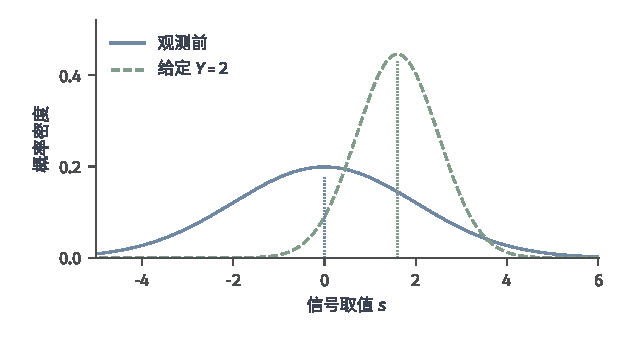
\includegraphics[width=105mm]{figures/02-mathematical-preliminaries-lower/01-random-variables-distributions-and-causality/matplotlib/probability-gaussian-observation-update/figure.pdf}
  \caption{独立高斯噪声下的一次观测更新。信号\(S\sim\mathcal N(0,4)\)，观测\(Y=S+\varepsilon\)，其中\(\varepsilon\sim\mathcal N(0,1)\)与\(S\)独立。蓝实线为\(S\)的先验密度，绿虚线为给定\(Y=2\)后的\(\mathcal N(1.6,0.8)\)密度；细竖线标出两者均值。}
  \label{fig:probability-gaussian-observation-update}
\end{figure}

多元高斯分布是一个特殊情形：联合高斯随机向量的两个子向量若协方差为零，则它们独立；条件高斯中的条件协方差为零也对应条件独立。这个结论依赖高斯
分布由一、二阶矩完全确定，不能推广到一般分布。


\subsubsection{高斯密度的乘积与多源信息合并}
\label{sec:probability-gaussian-density-products}
单个观测通过条件化改变高斯分布。若多项信息都以同一个未知量上的高斯密度表达，把这些密度相乘并归一化，也能得到闭式结果。这里相乘的是同一取值\(\bm x\)上的函数，并不是把多个随机向量相加。

\begin{theorem}[高斯密度乘积]
\label{prop:probability-gaussian-density-product}
设\(m\geq1\)，\(p_j\)是\(\mathbb R^d\)上均值\(\bm\mu_j\)、正定协方差\(\bm\Sigma_j\)的高斯密度。记精度矩阵\(\bm\Lambda_j=\bm\Sigma_j^{-1}\)。则
\[
 q(\bm x)=\frac{\prod_{j=1}^m p_j(\bm x)}{\int_{\mathbb R^d}\prod_{j=1}^m p_j(\bm z)\,\mathrm d\bm z}
\]
是高斯密度，其协方差与均值分别为
\begin{equation}
 \bm\Sigma=\left(\sum_{j=1}^m\bm\Lambda_j\right)^{-1},
 \qquad
 \bm\mu=\bm\Sigma\sum_{j=1}^m\bm\Lambda_j\bm\mu_j.
 \label{eq:probability-gaussian-density-product}
\end{equation}
\end{theorem}

\begin{proof}
乘积中各高斯指数的二次型之和为
\[
 \sum_j(\bm x-\bm\mu_j)^\top\bm\Lambda_j(\bm x-\bm\mu_j)
 =\bm x^\top\bm\Lambda\bm x-2\bm x^\top\bm h+c,
\]
其中\(\bm\Lambda=\sum_j\bm\Lambda_j\)、\(\bm h=\sum_j\bm\Lambda_j\bm\mu_j\)，\(c\)与\(\bm x\)无关。正定矩阵之和仍正定，因此可以配方为
\[
 (\bm x-\bm\Lambda^{-1}\bm h)^\top\bm\Lambda
 (\bm x-\bm\Lambda^{-1}\bm h)+c-\bm h^\top\bm\Lambda^{-1}\bm h.
\]
以该二次型构成的高斯函数关于\(\bm x\)的积分为有限正数。归一化以后，常数项相消，余下的密度正是式~\eqref{eq:probability-gaussian-density-product}中的高斯密度。
\end{proof}

一维时，均值按\(1/\sigma_j^2\)加权，方差为\((\sum_j1/\sigma_j^2)^{-1}\)。例如两个方差均为\(1\)、均值分别为\(0\)和\(2\)的密度，归一化乘积为\(\mathcal N(1,1/2)\)。乘积给出的方差变小，并不自动证明两项信息一致：即使把第二个均值改成\(10\)，方差仍为\(1/2\)。若数据来源存在相关性、模型失配或相互冲突，单凭这个代数运算不能把缩小的方差解释为可靠的推断精度。

多源后验合并还要检查先验是否重复计算。设\(\Theta\)有先验密度\(p_0\)，观测\(Y_1,\ldots,Y_m\)给定\(\Theta\)后条件独立，且各单源后验\(p_j(\theta\mid y_j)\)都采用同一个先验。由Bayes公式，在\(p_0(\theta)>0\)的支持上，
\begin{equation}
 p(\theta\mid y_1,\ldots,y_m)
 \propto p_0(\theta)\prod_jp(y_j\mid\theta)
 \propto p_0(\theta)^{1-m}\prod_jp_j(\theta\mid y_j).
 \label{eq:probability-common-prior-posterior-fusion}
\end{equation}
每个单源后验都含有一次先验；直接把它们相乘会把先验计入\(m\)次，因此要除去多出的\(m-1\)次。这个推导要求给定未知量后的条件独立，并要求所用后验、似然和归一化积分有定义。任意给出的高斯密度乘积总能按上面的命题归一化，但未必代表某组真实观测的共同后验。

\subsection{基于指数族的参数化表示}
% Baseline P:1018-1081
Poisson计数和高斯读数具有不同的取值空间，但其密度中的参数依赖都能集中到少量摘要与一个归一化项。指数族把这种共同结构写出来，使均值、协方差和似然计算能够复用同一组公式。
\begin{definition}[指数族]
  \label{def:probability-exponential-family}
在可测空间上固定一个\(\sigma\)有限参考测度\(\mu\)，非负可测基准项\(h\)和可测向量函数\(\bm T\)。一类由\(\bm{\eta}\)索引的分布若都被
\(\mu\)支配，且能写成
\begin{equation}
  \frac{\mathrm{d}P_{\bm{\eta}}}{\mathrm{d}\mu}(x)
  =
  h(x)\exp\left\{
    \bm{\eta}^{\top}\bm{T}(x)-A(\bm{\eta})
  \right\},
  \label{eq:probability-exponential-family}
\end{equation}
就称为\term{指数族}（exponential family）。其中\(\bm{\eta}\)是\term{自然参数}，\(\bm{T}(x)\)是充分统计量，\(h(x)\)是基准项。负责归一化的对数配分函数为
\[ A(\bm{\eta})
  =\log\int h(x)e^{\bm{\eta}^{\top}\bm{T}(x)}\,\mathrm{d}\mu(x), \]
自然参数空间由该积分严格为正且有限的参数组成；所用参数集合可以是这个空间的子集。
\end{definition}
这里“充分”可以先理解为：
样本取值中与参数\(\bm{\eta}\)有关的部分只通过摘要\(\bm{T}(x)\)进入密度；对独立同分布样本，相应摘要是
\(\sum_i\bm{T}(x_i)\)。充分性的正式定义与判据留到第~\ref{sec:statistics-likelihood-robustness}节。

离散分布通常取计数测度，此时积分就是求和；具有Lebesgue密度的分布取Lebesgue测度。因而Poisson分布与高斯分布都能由同一形式描述，但使用的参考测度不同。

若\(\bm{\eta}\)位于自然参数空间内部，并存在可积控制函数允许交换微分与积分，则
\[
\begin{aligned}
  \nabla A(\bm{\eta})
  &=
  \frac{\int \bm{T}(x)h(x)
  e^{\bm{\eta}^{\top}\bm{T}(x)}\,\mathrm{d}\mu(x)}
  {\int h(x)e^{\bm{\eta}^{\top}\bm{T}(x)}\,\mathrm{d}\mu(x)}\\
  &=
  \mathbb{E}_{\bm{\eta}}[\bm{T}(X)].
\end{aligned}
\]
再求一次导数得到
\begin{equation}
  \nabla^2 A(\bm{\eta})
  =
  \operatorname{Cov}_{\bm{\eta}}(\bm{T}(X)).
  \label{eq:probability-log-partition-hessian}
\end{equation}
自然参数空间的凸性来自Hölder不等式：两个有限归一化积分的几何插值仍有限。上述Hessian半正定进一步说明\(A\)在参数空间内部的凸性。若存在非零\(\bm a\)，使
\(\bm a^\top\bm T(X)\)几乎处处为常量，该方向的方差为零，Hessian矩阵就奇异。
这包括某个统计量恒为常量，以及一个统计量等于其余统计量的线性组合再加常数的情况；
严格凸性并不自动成立。

以Poisson分布为例，把密度写成\eqref{eq:probability-exponential-family}的形式即可读出参数：
\[ p_\lambda(x)
  =\frac{1}{x!}\exp\{x\log\lambda-\lambda\}. \]
自然参数为\(\eta=\log\lambda\)，充分统计量为\(T(x)=x\)，
基准项为\(h(x)=1/x!\)，配分函数为\(A(\eta)=e^\eta\)。于是
\[ A'(\eta)=e^\eta=\mathbb{E}X,
  \qquad A''(\eta)=e^\eta=\operatorname{Var}(X), \]
与Poisson分布的均值、方差一致。

这一步的做法可以固定下来：先整理指数部分，让参数只以「参数乘统计量」的乘积形式出现，
剩下的\(x\)部分归入\(h(x)\)，剩余常量归入\(A(\bm\eta)\)。按这个顺序核对下面两例，
就能看出\(A\)的导数为什么恰好给出矩。

Bernoulli分布提供另一个核对。取\(0<p<1\)，令\(\eta=\log(p/(1-p))\)，则
\[
  p_\eta(x)=\exp\{x\eta-\log(1+e^\eta)\},
  \qquad x\in\{0,1\}.
\]
所以\(A(\eta)=\log(1+e^\eta)\)，
\(A'(\eta)=p\)、\(A''(\eta)=p(1-p)\)，仍与Bernoulli分布的矩一致。
这里\(h(x)=1\)，全部参数依赖都进了指数，因此\(A\)必须同时承担归一化与矩计算两项任务。

已知方差\(\sigma^2>0\)的高斯分布更能说明\(h\)的作用。把密度指数上的平方展开为
\[
  -\frac{(x-\mu)^2}{2\sigma^2}
  =\frac{\mu}{\sigma^2}x-\frac{x^2}{2\sigma^2}-\frac{\mu^2}{2\sigma^2},
\]
第一项已经是「参数乘\(x\)」的形式，取\(\eta=\mu/\sigma^2\)、\(T(x)=x\)；第二项只含\(x\)，
归入基准项\(h(x)=\exp\{-x^2/(2\sigma^2)\}/\sqrt{2\pi\sigma^2}\)；第三项只含参数，移入配分函数得到
\(A(\eta)=\sigma^2\eta^2/2\)。于是
\(A'(\eta)=\sigma^2\eta=\mu\)、\(A''(\eta)=\sigma^2\)，均值与方差都被读出。
同一个分布的另一种抽样方式——多次独立观察——只需把\(T(x)\)换成样本和，
指数部分因此可加；这正是后文在独立样本下直接对统计量求和的原因。

这些例子说明，产生均值和协方差的是
\(\log\)配分函数\(A\)的导数，不是未取对数的归一化常数本身。写代码或查表时容易把两者
混用：密度前面的系数常随参数变化，但由它出发求导得不到矩，必须先把参数依赖整理进指数。

\section{随机变量的变换与生成}
\label{sec:rv-transformations}
\label{sec:probability-random-vectors-transformations}
由读数得到新随机对象，可以改变映射，也可以改变生成规律。把两台设备的读数相加，固定的是共同概率空间，变化的是取值函数；先确定设备状态再生成噪声，需要额外给出条件抽样规则；保持读数映射不变而重新分配事件概率，则改变基础权重。三种操作分别改变取值映射、条件生成规则与概率权重；随机序列和过程由第~\ref{chap:random-sequences-and-processes}章另行展开。

\subsection{基于取值映射的变换}
把几个读数合成一个新读数，是实际计算中最常见的操作：把两台设备的读数相加、相减，
取两者的最大或最小，都需要知道结果的分布。下面的规则先处理任意可测变换，
再给出可以逐项验算的情形。

\subsubsection{分布变换的一般规则}
\label{sec:rv-pushforward}
若\(X\)取值于\((E,\mathcal E)\)，\(g:E\to F\)可测，则
\(Y=g(X)\)的分布是\(P_Y=g_\#P_X\)，即
\[
P_Y(B)=P_X(g^{-1}(B)),\qquad
\mathbb E h(Y)=\int_E h(g(x))\,P_X(\mathrm dx)
\]
对非负可测\(h\)或可积\(h\)成立。这个规则不要求密度，也不要求\(g\)可逆。
% Baseline P:1187-1202
以下限制为同维欧氏空间：设\(\mathcal X,\mathcal Y\subseteq\mathbb R^d\)为开集，
\(\bm X\)在\(\mathcal X\)上相对于\(d\)维Lebesgue测度具有密度\(f_{\bm X}\)，
\(g:\mathcal X\to\mathcal Y\)为\(C^1\)微分同胚，即双射且它与逆映射都连续可微。
令\(\bm Y=g(\bm X)\)，换元公式给出输出相对于同维Lebesgue测度的密度
\begin{equation}
  f_{\bm{Y}}(\bm{y})
  =
  f_{\bm{X}}\bigl(g^{-1}(\bm{y})\bigr)
  \left|
    \det\bm{J}_{g^{-1}}(\bm{y})
  \right|.
  \label{eq:probability-density-change-variables}
\end{equation}
Jacobian矩阵的行列式补偿局部体积变化。只把\(x=g^{-1}(y)\)代入原密度而漏掉该因子，所得函数通常不能积分为\(1\)。

若映射可分为有限或可数个一一对应的\(C^1\)分支，各分支Jacobian非零，则在正则值处把各逆像分支的换元密度相加。一般可测映射仍应从推送测度定义出发。例如\(Y=X^2\)且\(X\)有密度时，对\(y>0\)，
\[ f_Y(y)
  =\frac{f_X(\sqrt{y})+f_X(-\sqrt{y})}{2\sqrt{y}}. \]
输出密度必须相对于输出空间的参考测度定义。输入与输出维数不同时，非方阵Jacobian不能直接取行列式换元。若
\((X_1,X_2)\)在单位正方形上均匀分布，投影\(g(x_1,x_2)=x_1\)降到一维，输出仍有一维密度\(1_{[0,1]}\)，由对\(x_2\)积分得到。相反，嵌入\(h(x)=(x,x)\)把一维变量放入二维，像落在直线上，没有二维Lebesgue密度。应比较输出支持与输出空间的维数，而不能把“降维”直接等同于“没有密度”。

\paragraph{概率积分变换与分位数复合}
\label{sec:probability-integral-transform}
换元公式逐点计算输出密度。有时只希望把一个已知分布改成另一个分布，可以先把输入变成累积概率，再用目标分位数把概率映回读数。这条路径直接使用分布函数，不需要对密度求导。

\begin{theorem}[概率积分变换与逆分位数生成]
\label{prop:probability-integral-transform}
若实随机变量\(X\)的分布函数\(F\)连续，则\(F(X)\sim\operatorname{Unif}[0,1]\)。对任意实数轴分布函数\(G\)，令\(G^{-1}(u)=\inf\{y:G(y)\geq u\}\)，其中\(0<u<1\)。若\(U\sim\operatorname{Unif}[0,1]\)，则\(G^{-1}(U)\)具有分布函数\(G\)。因此，当\(F\)连续时，\(G^{-1}(F(X))\)具有目标分布\(G\)；零概率的端点事件上可任取约定值。
\end{theorem}

\begin{proof}
固定\(0<u<1\)。由连续性及两端极限，集合\(\{x:F(x)\leq u\}\)有有限上端点\(b_u\)，并有\(F(b_u)=u\)。单调性给出\(\{F(X)\leq u\}=\{X\leq b_u\}\)，故其概率等于\(u\)。这证明第一条结论；证明不要求\(F\)严格递增，平坦区间不承载额外概率。

对目标分位数，分布函数的右连续性保证\(G^{-1}(u)\leq y\)当且仅当\(u\leq G(y)\)。所以
\[
 \mathbb P(G^{-1}(U)\leq y)=\mathbb P(U\leq G(y))=G(y),
\]
得到第二条结论。将第一条产生的均匀变量代入，便得到分位数复合结论。
\end{proof}

例如\(X\sim\operatorname{Unif}[0,2]\)时，\(F(X)=X/2\)。取目标为速率\(\lambda>0\)的指数分布，其分位数为\(G^{-1}(u)=-\log(1-u)/\lambda\)，于是\(-\log(1-X/2)/\lambda\)服从该指数分布。前一变换统一概率尺度，后一变换指定输出尺度。

若\(F\)有跳跃，\(F(X)\)一般不均匀。例如等概率取零或一的\(X\)，经过\(F\)后只取\(1/2\)与\(1\)，不会产生连续均匀分布。图像直方图均衡与匹配可借用这一构造，但有限灰度级的确定性映射不能把每个原子任意拆分，通常只能近似实现均衡；不能把连续情形的精确结论原样套用到离散直方图。

\subsubsection{随机变量的组合与排序}
\label{sec:rv-combinations}
把两个读数相加或加权组合，结果的不确定程度是多少？平均值可以直接相加，波动却要
看两部分的共同变化。
可积变量的和满足\(\mathbb E(X+Y)=\mathbb EX+\mathbb EY\)，不需要独立；
二阶可积时
\[
\operatorname{Var}(aX+bY)
=a^2\operatorname{Var}(X)+b^2\operatorname{Var}(Y)
 +2ab\operatorname{Cov}(X,Y).
\]
第三项就是共同变化带来的修正：同向变化时相加，反向变化时相消。
图~\ref{fig:rv-dependence}中三个和的方差依次为\(1,1/2,0\)。相同边缘并没有给出相同的累计波动。若只知两个变量可积，乘积未必可积；二阶可积则由Cauchy--Schwarz保证乘积可积。比值还须确保分母非零，且另查比值的矩。

\paragraph{信号相关噪声的均值与方差}
固定非负信号强度\(x\)，设读数为
\[
 Y=\alpha N+\varepsilon,\qquad
 N\sim\operatorname{Poisson}(x/\alpha),\qquad
 \varepsilon\sim\mathcal N(0,\sigma^2),
\]
其中\(\alpha>0\)、\(\sigma^2>0\)，且\(N\)与\(\varepsilon\)独立。\(N\)表示随机计数，\(\alpha\)把一次计数换算为读数增量，\(\varepsilon\)表示独立的加性读出误差；当\(x=0\)时约定\(N=0\)几乎处处。这个泊松—高斯噪声（Poisson–Gaussian noise）模型可用于近似描述尚未经过复杂处理的传感器读数\scite{vision-foi2008}。

Poisson变量的均值与方差均为\(x/\alpha\)，独立性又使交叉协方差为零，因而
\begin{equation}
 \mathbb E Y=x,\qquad
 \operatorname{Var}(Y)=\alpha x+\sigma^2,
 \qquad
 \mathbb E[(Y-x)^2]=\alpha x+\sigma^2.
 \label{eq:probability-poisson-gaussian-moments}
\end{equation}
最后一项是读数相对固定信号\(x\)的均方误差；这里均值等于目标，所以它与方差相等。即使加性读出噪声方差固定，总误差方差仍随信号增加。作为教学计算，取\(\alpha=1\)、\(\sigma=2\)，\(x=4\)与\(x=100\)的标准差分别为\(\sqrt8\)与\(\sqrt{104}\)，信号除以标准差分别约为\(1.41\)与\(9.81\)。绝对波动增大与相对误差降低可以同时发生；不能用一个固定方差的加性噪声模型覆盖这两个强度下的规律。


\paragraph{相关读数的加权组合}
这一修正对重复测量的效果值得单独算一次。设两次读数\(X_1,X_2\)同方差
\(\operatorname{Var}(X_i)=\sigma^2\)、相关系数为\(\rho\)，取两者平均
\(\bar X=(X_1+X_2)/2\)。按上式取\(a=b=1/2\)，得
\[
  \operatorname{Var}(\bar X)
  =\frac{\sigma^2}{4}+\frac{\sigma^2}{4}
   +2\cdot\frac14\rho\sigma^2
  =\frac{\sigma^2(1+\rho)}2.
\]
\(\rho=0\)时方差降为一半，这正是“多测几次更准”的依据；\(\rho=1\)时结果是
\(\sigma^2\)，与只测一次无异。只报告样本量而不报告相关性，就无法判断平均是否
真的降低了波动，这也说明成批出现的测量偏差无法靠增多样本消除。权重不等时第二项按
权重平方减少、第三项按权重乘积变化，两者比例不同，因此可靠但相关的读数应当给予
多少权重，需要代入具体数值比较，不能只凭哪一次读数更可靠来判断。

\paragraph{和、乘积与比值的分布}
若\(X,Y\)具有联合密度\(f_{X,Y}\)，换元与边缘化给出
\[
\begin{aligned}
f_{X+Y}(s)&=\int_{\mathbb R}f_{X,Y}(x,s-x)\,\mathrm dx,\\
f_{XY}(z)&=\int_{\mathbb R\setminus\{0\}}
 f_{X,Y}(x,z/x)\frac{\mathrm dx}{|x|},\\
f_{X/Y}(r)&=\int_{\mathbb R}|y|f_{X,Y}(ry,y)\,\mathrm dy.
\end{aligned}
\]
后两式的Jacobian因子分别为\(1/|x|\)和\(|y|\)。独立时联合密度可分解，和的密度便是卷积\(f_X*f_Y\)；离散和相应使用
\(\mathbb P(X+Y=s)=\sum_x\mathbb P(X=x)\mathbb P(Y=s-x)\)。
例如独立标准高斯之比\(R=X/Y\)满足
\[
f_R(r)=\frac1{2\pi}\int_{\mathbb R}|y|
 e^{-(1+r^2)y^2/2}\,\mathrm dy
=\frac1{\pi(1+r^2)}.
\]
这是标准Cauchy密度，\(\mathbb E|R|=\infty\)。分子分母都拥有全部矩，也不保证比值有均值。

\paragraph{独立和的变换函数}
独立性还把变换函数化为乘积：
\[
\varphi_{X+Y}(t)=\mathbb E(e^{\mathrm itX}e^{\mathrm itY})
=\varphi_X(t)\varphi_Y(t).
\]
在矩母函数共同有限的邻域，同样有
\(M_{X+Y}=M_XM_Y\)、\(K_{X+Y}=K_X+K_Y\)。向量的独立坐标使联合累积量生成函数按坐标相加，因此所有涉及至少两个不同坐标的累积量都为零。
反过来，若联合累积量生成函数在原点邻域解析，且这些跨坐标累积量全部为零，其Taylor展开就没有混合项。
又因\(K_{\bm X}(\bm0)=0\)，剩下的各组单坐标项分别等于边缘累积量生成函数，从而
\[
 K_{\bm X}(\bm t)=\sum_jK_{X_j}(t_j),\qquad
 M_{\bm X}(\bm t)=\prod_jM_{X_j}(t_j).
\]
右侧也是边缘乘积测度的矩母函数；由定理~\ref{thm:rv-transform-uniqueness}，联合分布等于该乘积测度，故坐标独立。
这里只让有限几个混合累积量为零还不够。高阶累积量可识别协方差未反映的非高斯依赖，纯高斯的三阶及以上累积量则为零。
独立Poisson变量的矩母函数为
\(\exp\{\lambda(e^t-1)\}\)，相乘后参数相加；独立标准高斯平方的Gamma矩母函数相乘，则得到前面定义的卡方分布。

\paragraph{仿射变换与白化}
对向量，令\(\bm Y=\bm A\bm X+\bm b\)，相应矩存在时
\[
\mathbb E\bm Y=\bm A\bm\mu+\bm b,\quad
\operatorname{Cov}(\bm Y)=\bm A\bm\Sigma\bm A^\top,\quad
\operatorname{Cov}(\bm A\bm X,\bm B\bm X)=\bm A\bm\Sigma\bm B^\top.
\]
前两条不要求高斯性。若\(\bm X\)联合高斯，则任意线性组合仍高斯，因而
\(\bm Y\sim\mathcal N(\bm A\bm\mu+\bm b,\bm A\bm\Sigma\bm A^\top)\)，即使\(\bm A\)不满秩也成立，但不能因此写出非退化密度。

协方差变换式也说明了白化（whitening）的含义：对中心化向量作线性变换，使协方差成为单位阵。若\(\bm\Sigma\succ\bm0\)，可取
\(\bm Y=\bm\Sigma^{-1/2}(\bm X-\bm\mu)\)；此后任何正交旋转\(\bm Q\bm Y\)仍有单位协方差，因为\(\bm Q\bm I\bm Q^\top=\bm I\)。
因此二阶统计量无法继续辨认这些旋转方向。独立成分分析（independent component analysis, ICA）希望从若干源信号的线性混合观测中，辨认相互独立的源。
源具有适当的非高斯性时，高阶统计量可以提供白化后仍缺少的方向信息；纯高斯的三阶及以上累积量全为零，不能承担这一任务。这里说明的是高阶信息的用途，并不保证任意三阶、四阶量都足以唯一识别源。

\paragraph{排序与顺序统计量}
排序也是函数变换。取正整数\(n\)和\(1\leq k\leq n\)。若\(X_1,\ldots,X_n\)独立同分布，分布函数为\(F\)，则
\[
\mathbb P(\max_iX_i\leq x)=F(x)^n,\quad
\mathbb P(\min_iX_i>x)=(1-F(x))^n,
\]
\[
\mathbb P(X_{(k)}\leq x)
=\sum_{j=k}^n\binom njF(x)^j(1-F(x))^{n-j}.
\]
这里把“第\(k\)小不超过\(x\)”改写成至少\(k\)个输入不超过\(x\)，所以出现二项计数。
% Baseline T:963-968
对次序统计量\(Y_{(1)}\leq\cdots\leq Y_{(n)}\)，经验分位数由相应秩位置给出。
若\(Y_1,\ldots,Y_n\)是来自连续分布\(F\)的独立同分布样本，则
\(F(Y_{(k)})\)服从
\(\operatorname{Beta}(k,n+1-k)\)，因此可以用秩而不是高斯近似构造分位数区间。
对离散或混合分布，跳跃与平坦区间都要求覆盖计算保留定义中的不等式方向。

\subsection{基于条件分布的随机生成}
\label{sec:rv-random-generation}
\subsubsection{基于类别选择的混合生成}
% Baseline P:1206-1253
有时读数来自几类未直接标记的来源，例如同一批产品由两条产线分别生产，误差规律并不相同。混合模型先抽取离散指标\(Z\)表示来自哪一类，再从该类的分量分布生成\(X\)：
\[ p(x)=\sum_{k=1}^{K}\mathbb{P}(Z=k)p(x\mid Z=k). \]
边缘化\(Z\)得到混合密度，条件化\(X\)则得到分量责任概率。潜变量不必对应可观测的真实类别；它本质上是组织联合分布和计算的数学变量。

混合分布的方差同时包含分量内和分量间变化。若
\(\mathbb{P}(Z=1)=1/4\)、\(\mathbb{P}(Z=2)=3/4\)，且
\[
  X\mid Z=1\sim\mathcal{N}(-1,1),\qquad
  X\mid Z=2\sim\mathcal{N}(1,1),
\]
则\(\mathbb{E}X=(-1)/4+3/4=1/2\)。全方差公式给出
\[
  \operatorname{Var}(X)
  =\underbrace{\mathbb{E}[\operatorname{Var}(X\mid Z)]}_{1}
   +\underbrace{\operatorname{Var}(\mathbb{E}[X\mid Z])}_{3/4}
  =\frac74.
\]
只平均两个分量方差会漏掉均值差造成的\(3/4\)。

\subsubsection{基于随机参数的层次生成}
有限混合用类别指标选择分量。若要让多个读数共享一个随机参数，可以先生成该参数，再按参数所决定的条件分布生成有限个读数。这样的层次模型（hierarchical model）把参数本身也作为随机对象，例如
\[ \Theta\sim\pi,\qquad
  X_i\mid\Theta\mathrel{\overset{\mathrm{ind}}{\sim}}p_\Theta,\qquad i=1,\ldots,n. \]
给定\(\Theta\)时，观测条件独立；边缘化共同参数后，观测通常相关。把“条件独立”
误写成“边缘独立”会丢掉层次模型中共享不确定性的主要作用。有限混合也能写成一类层次构造；这里的区别是当前把哪一项作为条件，以及多个读数是否共享这项条件。

例如设\(\Theta\)具有有限正方差，令\(X_1=\Theta+\varepsilon_1\)、\(X_2=\Theta+\varepsilon_2\)，其中两个噪声零均值、二阶可积，且彼此独立并独立于\(\Theta\)。给定\(\Theta\)后，两项噪声仍独立，所以\(X_1,X_2\)条件独立；不固定该参数时，展开协方差得到\(\operatorname{Cov}(X_1,X_2)=\operatorname{Var}(\Theta)>0\)。条件内的生成规则与条件之间的共同变化因此承担不同作用。

\subsection{基于概率重加权的分布变换}

保持同一个取值函数\(g\)，把事件权重从\(\mu\)改成\(\nu\)，会改变它的积分。若\(\nu\ll\mu\)，第~\ref{sec:probability-radon-nikodym-change-measure}节已经给出密度比\(r\)。现在把这个比值直接乘入旧积分，便能计算新权重下的平均。
\label{sec:rv-change-measure}
\subsubsection{密度比与换测度积分}
% Baseline P:249-302
\begin{theorem}[换测度积分公式]
\label{thm:probability-change-measure-integral}
若\(\nu\ll\mu\)，\(r=\mathrm{d}\nu/\mathrm{d}\mu\)，则对每个非负可测函数\(g\)，
\[ \int g\,\mathrm{d}\nu
  =\int gr\,\mathrm{d}\mu. \]
只要\(g\)在\(\nu\)下可积，同一等式也对实值\(g\)成立。
\end{theorem}

\begin{proof}
对指示函数\(g=\mathbb{I}_A\)，结论就是Radon--Nikodym表示。由线性性，它对非负简单函数成立。任取非负可测\(g\)，选择简单函数\(g_n\uparrow g\)，分别在
\(\nu\)和\(\mu\)下使用单调收敛定理即可。对可积实值函数，再分别处理\(g^+\)与\(g^-\)。
\end{proof}

密度比存在、有界和具有有限二阶矩是三项不同条件。若\(P\ll Q\)，则\(w=\mathrm{d}P/\mathrm{d}Q\)存在且\(\mathbb{E}_Q[w]=1\)，但这不推出
\(\lVert w\rVert_\infty<\infty\)，也不推出\(\mathbb{E}_Q[w^2]<\infty\)。例如在\((0,1)\)上令\(Q\)为均匀分布，取
\[ w(x)=\frac{1}{2\sqrt{x}}. \]
它的积分为\(1\)，所以定义一个\(P\ll Q\)；但\(w\)无界，且\(\int_0^1w(x)^2\,\mathrm{d}x=\infty\)。换测度恒等式仍成立，使用该权重的蒙特卡洛估计却可能没有有限方差。

有限表可以直接核对权重方向。设参考分布\(Q\)在三个结果上的概率为
\((0.5,0.4,0.1)\)，目标分布\(P\)为\((0.2,0.3,0.5)\)，则
\[
  w=\frac{\mathrm{d}P}{\mathrm{d}Q}=(0.4,0.75,5).
\]
对取值\(g=(1,2,4)\)，有
\[
  \mathbb{E}_P[g]=2.8
  =0.5(0.4)(1)+0.4(0.75)(2)+0.1(5)(4)
  =\mathbb{E}_Q[wg].
\]
第三个结果在\(Q\)下少见，却在\(P\)下承载一半质量，所以产生大权重。若把参考概率
\(0.1\)改成\(0\)而保持目标概率\(0.5\)，则\(P\not\ll Q\)，任何重加权都无法从
\(Q\)样本恢复这部分目标质量。

图~\ref{fig:probability-importance-weights}显示，权重改变的是每个结果对平均的贡献，而不是把观测值\(g_j\)解释为概率。未加权平均为\(1.7\)，加权平均为\(2.8\)；第三个结果的贡献从\(0.4\)增至\(2\)，也预示它偶尔出现时会显著推动估计值。

\begin{figure*}[htbp]
  \centering
  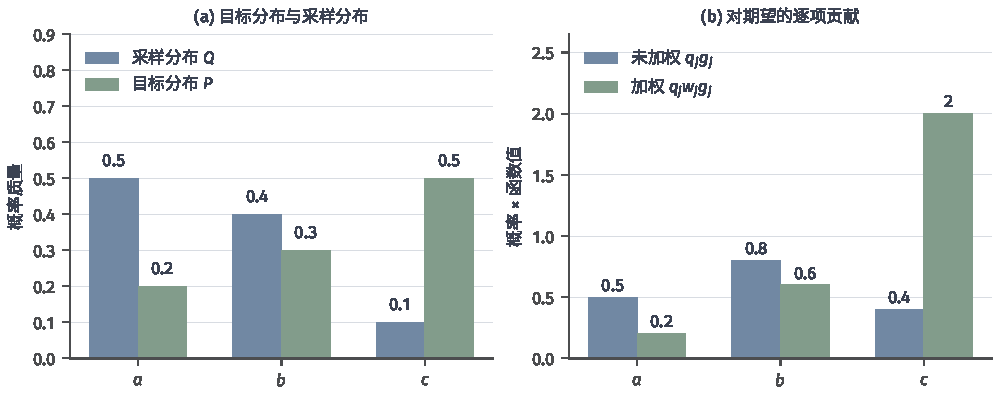
\includegraphics[width=\linewidth]{figures/02-mathematical-preliminaries-lower/01-random-variables-distributions-and-causality/matplotlib/probability-importance-weights/figure.pdf}
  \caption{三结果换测度的有限构造。左图比较采样分布\(Q\)与目标分布\(P\)，右图比较\(q_jg_j\)与\(q_jw_jg_j=p_jg_j\)。各柱从零起画；右图柱高之和分别为\(1.7\)和\(2.8\)，并非单点概率。}
  \label{fig:probability-importance-weights}
\end{figure*}

绝对连续性也决定几乎处处结论能否转移。若\(P\ll Q\)，且
\(|g|\leq M\)在\(Q\)下几乎处处成立，则违背上界的集合是\(Q\)-零集，因而也是
\(P\)-零集；同一上界在\(P\)下仍成立。反向转移需要\(Q\ll P\)，不能只凭
\(P\ll Q\)得到。若\(|g|\leq B\)，则
\[
  \mathbb{E}_Q[w^2g^2]\leq B^2\mathbb{E}_Q[w^2],
\]
所以权重二阶矩有限是有界被积函数获得有限重加权方差的充分条件。把权重截为
\(w_c=\min\{w,c\}\)会限制波动，但
\(\mathbb{E}_Q[w_cg]\)与\(\mathbb{E}_P[g]\)之差为
\(-\mathbb{E}_Q[(w-c)_+g]\)，一般不为零。

\subsubsection{条件期望的重加权与归一化}
% Baseline P:628-716
设\(Q\ll P\)，并记\(L=\mathrm{d}Q/\mathrm{d}P\)。对\(X\in L^1(Q)\)，在\(\mathbb{E}_P[L\mid\mathcal{G}]>0\)处有
\begin{equation}
  \mathbb{E}_Q[X\mid\mathcal{G}]
  =
  \frac{\mathbb{E}_P[LX\mid\mathcal{G}]}
       {\mathbb{E}_P[L\mid\mathcal{G}]}.
  \label{eq:probability-conditional-change-measure}
\end{equation}
为验证这个候选变量确实是条件期望，记
\[
  D=\mathbb{E}_P[L\mid\mathcal{G}],
  \qquad
  N=\mathbb{E}_P[LX\mid\mathcal{G}],
\]
并在\(\{D>0\}\)上令\(Z=N/D\)，在\(\{D=0\}\)上令\(Z=0\)。分母零集在\(Q\)下可以忽略，因为
\[
  Q(D=0)
  =
  \mathbb{E}_P[L\mathbb{I}\{D=0\}]
  =
  \mathbb{E}_P[D\mathbb{I}\{D=0\}]
  =0.
\]
条件期望的单调性还给出
\[
  |N|
  \leq
  \mathbb{E}_P[L|X|\mid\mathcal{G}].
\]
在\(\{D=0\}\)上，非负变量\(L\mathbb{I}\{D=0\}\)的期望为零，因而\(L=0\)几乎处处。于是
\[
  \mathbb{E}_P\left[
    \mathbb{E}_P[L|X|\mid\mathcal{G}]
    \mathbb{I}\{D=0\}
  \right]
  =
  \mathbb{E}_P[L|X|\mathbb{I}\{D=0\}]
  =0,
\]
上面的条件三角不等式进而说明\(N=0\)在\(\{D=0\}\)上几乎处处成立。因此\(DZ=N\)几乎处处，而且
\[
  \begin{aligned}
    \mathbb{E}_Q|Z|
    &=
    \mathbb{E}_P[L|Z|]
    =
    \mathbb{E}_P[D|Z|]\\
    &=
    \mathbb{E}_P\bigl[|N|\mathbb{I}\{D>0\}\bigr]
    \leq
    \mathbb{E}_P[L|X|]
    =
    \mathbb{E}_Q|X|<\infty.
  \end{aligned}
\]
这里把\(\mathcal{G}\)-可测的非负因子\(|Z|\)提出条件期望，可以由有界截断和单调收敛得到。候选变量的可积性建立后，对
\(A\in\mathcal{G}\)可合法地计算
\[
  \begin{aligned}
    \int_A Z\,\mathrm{d}Q
    &=
    \int_A ZL\,\mathrm{d}P
    =
    \int_A Z\mathbb{E}_P[L\mid\mathcal{G}]\,\mathrm{d}P\\
    &=
    \int_A \mathbb{E}_P[LX\mid\mathcal{G}]\,\mathrm{d}P
    =
    \int_A LX\,\mathrm{d}P
    =
    \int_A X\,\mathrm{d}Q.
  \end{aligned}
\]
因此\(Z\)满足\(X\)在\(Q\)下关于\(\mathcal{G}\)的条件期望定义。公式\eqref{eq:probability-conditional-change-measure}是Bayes更新的一般测度形式；
分母零集与候选变量可积性都需要像上面这样核对。

用有限分组可以看出分母为何不可省略。设参考分布\(P\)把四个结果
\(\omega_1,\ldots,\omega_4\)分别赋予概率\((0.4,0.1,0.1,0.4)\)，目标分布
\(Q\)赋予\((0.1,0.5,0.1,0.3)\)。令信息\(\mathcal{G}\)只区分
\(A=\{\omega_1,\omega_2\}\)和\(A^{\mathsf c}\)，并令
\(X=(0,1,0,1)\)。权重\(L\)在四点上的值为\((0.25,5,1,0.75)\)。在\(A\)内，
\[
  \mathbb{E}_P[LX\mid\mathcal{G}]
  =\frac{0.5}{0.5}=1,\qquad
  \mathbb{E}_P[L\mid\mathcal{G}]
  =\frac{0.1+0.5}{0.5}=1.2,
\]
所以目标条件均值为\(1/1.2=5/6\)，与
\(\mathbb{E}_Q[X\mid A]=0.5/(0.1+0.5)\)一致。
省略分母却会得到\(1\)，可以直接看到重新归一化改变了答案。
在\(A^{\mathsf c}\)内，分子为\(0.3/0.5=0.6\)，分母为\(0.4/0.5=0.8\)，
相除得到\(3/4\)，也等于该组在\(Q\)下的条件均值。
条件化后必须按每个信息分组的目标总质量分别归一化。

\section{单个随机变量的尾概率控制}
\label{sec:probability-elementary-tail-bounds}
\subsection{非负随机变量的Markov不等式}
如果一个非负随机变量经常超过阈值，它的平均值就不能太小。这一关系使我们能从已知的一阶矩控制大取值事件。设非负随机变量为\(X\)，阈值为\(a>0\)，则
\begin{equation}
  \mathbb{P}(X\geq a)
  \leq
  \frac{\mathbb{E}X}{a}.
  \label{eq:probability-markov-inequality}
\end{equation}
证明只需写
\(\mathbb{E}X\geq
\mathbb{E}[X\mathbb{I}\{X\geq a\}]
\geq a\mathbb{P}(X\geq a)\)。
这就是Markov不等式。

\subsection{有限方差下的Chebyshev不等式}
对均值\(\mu\)、方差\(\sigma^2<\infty\)的随机变量，把
Markov不等式用于\((X-\mu)^2\)，得到Chebyshev不等式
\begin{equation}
  \mathbb{P}(|X-\mu|\geq t)
  \leq\frac{\sigma^2}{t^2},
  \qquad t>0.
  \label{eq:probability-chebyshev-inequality}
\end{equation}
它只使用二阶矩，因而适用范围广，但没有利用有界性或指数矩信息。

\section{本章小结}
\label{sec:probability-summary}
传感器的一次读数既是一项确定的取值规则，也是在概率空间上定义的随机变量。分布测度把基础结果合并为读数事件，分布函数、参考密度与积分变换则提供不同的完整表示。密度需要绝对连续等存在条件，矩母函数需要指数矩条件；均值、方差和有限个矩通常只能保留部分信息。

两台设备具有相同边缘分布，不代表平均读数具有相同波动。联合分布决定协方差与共同事件的概率；条件分布回答获得信息后的查询，条件均值在平方可积条件下给出最优平方损失预测。独立与条件独立允许积分分解，零协方差在一般分布中不足以代替它们；联合高斯是在一、二阶矩之外加入完整分布结构的一种特殊模型。

由读数得到新分布时，应先辨认改变的是哪一个对象。取值映射改变输出，条件生成保留给定条件下的随机性，概率重加权改变同一事件的概率。换元需要核对支持与维数，重加权需要核对零集和可积性。基本Markov与Chebyshev界把矩信息转成尾事件保证；反复采样的集中与极限，以及从有限数据推断未知规律，还要在后续章节增加相应条件。

\chapter{概率分布}
\label{chap:information-theory-and-statistical-geometry}

记录一串随机结果时，常见结果可以用短码，罕见结果需要较长描述。预测这些结果时，
给真实结果分配过小的概率又会增加描述代价。这两个问题都涉及概率，却不相同：
前者问一个规律本身有多少不确定性，后者问用另一个规律代替它会付出多少代价。
若预测的是温度，还会出现第三个问题：整体偏移\(0.1\)度与把少量概率移到极端温度，
对平均误差和越界概率的影响是否相同？

第~\ref{chap:probability-theory}章已经说明分布怎样由随机变量产生，以及怎样条件化和换测度。现在把概率分布本身作为比较或优化对象：信息量描述一张规律中的不确定性，分布差异比较两张规律给出的概率、期望和位置，分布区分则判断观测能否辨认候选规律。

固定评价函数以后，分布变化会改变其期望；把分布作为未知量时，收益、表示或边缘约束又决定可选规律。参数更新需要服从这些约束及分布几何。完成这些分析后，本章再回到样本评价：评价对象根据同一批样本选出时，怎样用联合依赖和同时概率事件控制评价误差。

参数相近也不能替代分布相近。高斯均值移动相同距离，在噪声较小时更容易被辨认；
把均值改用立方根表示，还会改变参数的欧氏距离。因而先要确定比较什么，
才能判断一个小差异是否足以保护任务结果，或怎样约束一次参数更新。
除编码处显式使用\(\log_2\)外，本章的\(\log\)均为自然对数，单位为nat；
以二为底时单位为bit，\(1\ \mathrm{bit}=(\log2)\ \mathrm{nat}\)。

\section{观测的信息量}
\label{sec:information-uncertainty-prediction}

设一串记录按已知规律产生，常见结果会反复出现。给常见结果短码、罕见结果长码，可以降低每条记录的平均描述长度；这个平均由出现概率决定。若另一个变量已经被观察，还可以只描述剩余的不确定部分。离散结果能够直接对应码字，连续结果则要同时规定记录精度。

\Needspace{7\baselineskip}
\subsection{离散观测的信息量}
\label{sec:information-entropy}

\subsubsection{无条件观测的平均信息量}
\label{sec:information-unconditional-information}

设结果\(x\)的发生概率为\(p(x)>0\)。两个独立结果的联合概率相乘，而描述长度应相加，
这使负对数成为自然的计量方式。\term{自信息}（self-information）
\(-\log p(x)\)表示看到这次结果时的意外程度：概率越小，数值越大。
它是单次结果的量，尚未对所有可能结果平均。

\begin{definition}[离散熵]
\label{def:information-discrete-entropy}
设离散随机变量\(X\)取值于有限或可数字母表\(\mathcal X\)，质量函数为\(p\)。
其\term{熵}（entropy）是自信息的平均：
\begin{equation}
  H(X)=-\sum_{x\in\mathcal X}p(x)\log p(x)
      =\mathbb E[-\log p(X)].
  \label{eq:information-discrete-entropy}
\end{equation}
约定\(0\log0=0\)。这是非负扩展值求和，可以为\(+\infty\)。
熵有限的条件可写为
\[
  \sum_xp(x)|\log p(x)|<\infty.
\]
\end{definition}

常量没有待区分的结果，熵为零；\(m\)个等概率结果的熵为\(\log m\)。
例如\(X\sim\operatorname{Bernoulli}(1/4)\)时，
\[
  H(X)=-\tfrac14\log\tfrac14-\tfrac34\log\tfrac34
       \approx0.5623\ \mathrm{nat}\approx0.8113\ \mathrm{bit}.
\]
结果\(1\)的自信息为\(2\) bit，但它只占四分之一的发生概率，所以平均值不到一位。
这个平均数能否真的变成码长，要同时检查码字能否解码。

二进制前缀码（prefix code）要求任何码字都不是另一个码字的前缀，
因此串接后可以逐个解析。码字\(0,10,11\)满足这一要求，\(0,01\)则不满足。
若码长为非负整数\(\ell(x)\)，把长度为\(\ell\)的码字看成二叉树深度\(\ell\)
的节点，它占据的后代比例是\(2^{-\ell}\)。前缀码所占的后代不能重叠，故
\[
  \sum_x2^{-\ell(x)}\leq1.
\]
这就是Kraft约束。理想实数码长\(-\log_2p(x)\)恰好使总和为一，
实际码长则还要满足整数约束\scite{math-cover2006information}

\begin{theorem}[无失真前缀码的平均长度界]
\label{thm:information-source-coding-bound}
对熵有限的质量函数\(p\)，任意满足Kraft约束的二进制码长均满足
\[
  \mathbb E\ell(X)\geq H(X)/\log2.
\]
在有效字母表\(\mathcal X_+=\{x:p(x)>0\}\)上，
\(\ell(x)=\lceil-\log_2p(x)\rceil\)可由前缀码实现，并且
\[
  \mathbb E\ell(X)<H(X)/\log2+1.
\]
\end{theorem}
\begin{proof}
若平均码长无限，下界直接成立。否则令
\(K=\sum_x2^{-\ell(x)}\in(0,1]\)、\(q(x)=2^{-\ell(x)}/K\)。
由\(-\log u\geq1-u\)，在\(p>0\)的点上求和得到
\[
  \sum_xp(x)\log\frac{p(x)}{q(x)}
  \geq1-\sum_{x:p(x)>0}q(x)\geq0.
\]
所以
\[
  0\leq-H(X)+(\log2)\mathbb E\ell(X)+\log K.
\]
因\(\log K\leq0\)，移项即得下界。这里直接证明所需的对数不等式，
没有预先使用后文才定义的KL。

对取整码长，\(2^{-\ell(x)}\leq p(x)\)，故满足Kraft约束。
按码长非降排列有效字母表，依次在\([0,1)\)放置长度\(2^{-\ell(x)}\)
的半开二进区间。此前区间长度都是当前长度的整数倍，因此新左端点仍与当前
二进网格对齐；总长度不超过一，区间都能放下。以左端点的前\(\ell(x)\)个
二进位为码字。若一个码字是另一个的前缀，相应二进区间便会嵌套，
与区间互不相交矛盾。这个构造也适用于可数字母表，因为每个有限码长下只能有有限个码字。
再对\(\lceil a\rceil<a+1\)平均，得到严格上界。
\end{proof}

Bernoulli例子的两个有效结果都必须使用至少一位，逐符号码长为\(1\) bit；
与\(0.8113\) bit的差来自整数限制。对独立的\(n\)个结果一起编码，
块熵为\(nH(X)\)，每符号冗余可小于\(1/n\) bit。零质量符号已从有效字母表删除；
若也必须传输它们，要额外留出码空间。只有一个有效符号时，上述约定允许空码字，
并假定符号个数已知。允许重建失真则是另一任务，码长还依赖失真准则，
不能仅由熵决定。

\subsubsection{条件观测的剩余信息量}
\label{sec:information-remaining-information}

若发送者和接收者都知道\(Y=y\)，需要描述的是条件分布\(p(x\mid y)\)，
而不是重新描述整个\(X\)。前章的条件分布使这一点可以逐个条件值计算。

\begin{definition}[离散条件熵]
\label{def:information-conditional-entropy}
对离散随机变量\(X,Y\)，在\(p(y)>0\)处令
\(H(X\mid Y=y)=-\sum_xp(x\mid y)\log p(x\mid y)\)。
\term{条件熵}（conditional entropy）定义为这些剩余信息量的平均：
\begin{equation}
  H(X\mid Y)=\sum_yp(y)H(X\mid Y=y)
           =-\sum_{x,y}p(x,y)\log p(x\mid y).
  \label{eq:information-conditional-entropy}
\end{equation}
零质量条件值可以任意指定条件分布，贡献为零；结果允许为\(+\infty\)。
\end{definition}

在联合质量为正的点，\(p(x,y)=p(y)p(x\mid y)\)。
对负对数取期望得到
\[
\begin{aligned}
  H(X,Y)
  &=-\sum_{x,y}p(x,y)\log p(y)
    -\sum_{x,y}p(x,y)\log p(x\mid y)\\
  &=H(Y)+H(X\mid Y).
\end{aligned}
\]
这些项非负，非负求和换序保证等式在扩展值意义下也成立。
反复分解给出联合熵的链式法则：
\begin{equation}
  H(X_1,\ldots,X_n)
  =\sum_{i=1}^nH(X_i\mid X_1,\ldots,X_{i-1}).
  \label{eq:information-entropy-chain-rule}
\end{equation}
链式法则不要求独立；独立时各条件熵才可换成无条件熵。
若要移项写成熵之差，必须确认相应熵有限，不能计算\(\infty-\infty\)。

\begin{example}[一次带噪二元观测]
\label{ex:information-binary-channel}
令\(X\)在\(\{0,1\}\)上均匀，观测\(Y=X\oplus N\)，其中\(\oplus\)为异或，
\(N\sim\operatorname{Bernoulli}(\varepsilon)\)独立于\(X\)，
\(0\leq\varepsilon\leq1/2\)。对每个\(y\)，
\[
  P(X=y\mid Y=y)=1-\varepsilon,\qquad
  P(X=1-y\mid Y=y)=\varepsilon.
\]
定义二元熵函数
\(H_{\mathrm b}(u)=-u\log u-(1-u)\log(1-u)\)，端点沿用零项约定。
于是\(H(X)=\log2\)、\(H(X\mid Y)=H_{\mathrm b}(\varepsilon)\)。
当\(\varepsilon=1/4\)时，观测后剩余\(0.5623\) nat，
比观测前少\(0.1308\) nat；无噪声时没有剩余不确定性，
公平翻转时则仍剩全部\(\log2\) nat。
\end{example}

这里计算的是条件分布下的平均剩余量，不是每次观测都能准确恢复的保证。
减少部分怎样描述两个变量的关系，将在第~\ref{sec:information-mutual-relations}节
用一般测度上的分布比较给出定义，并画出此例随噪声变化的原图。

\subsection{连续观测的信息量}
\label{sec:information-continuous-information}

连续结果若要求无限精度，单次记录通常不能用有限比特无失真描述。
可以先把实轴分成宽度\(\Delta\)的小格；在密度足够规则时，
格子概率近似\(p(x)\Delta\)，格子编码熵便近似
\(-\int p\log p-\log\Delta\)。精度代价\(-\log\Delta\)需要单独保留，
余下的密度项才是微分熵。这个近似用于解释口径，并非对任意密度都成立的量化极限定理。

\begin{definition}[微分熵]
\label{def:information-differential-entropy}
固定参考测度\(\mu\)。若\(P\ll\mu\)、\(p=\mathrm dP/\mathrm d\mu\)，且
\(\mathbb E_P|\log p(X)|<\infty\)，定义相对于\(\mu\)的熵
\[
  h_\mu(P)=-\int p\log p\,\mathrm d\mu.
\]
在\(\mathbb R^d\)上取Lebesgue测度时，称为\term{微分熵}
（differential entropy），简记为\(h(\bm X)\)。
\end{definition}

指定参考测度是定义的一部分。若换成\(\mu'=a\mu\)，其中\(a>0\)，
密度变为\(p/a\)，故\(h_{\mu'}(P)=h_\mu(P)+\log a\)。
与离散质量不同，密度可能大于一，其负对数也可能为负。
例如\(X\)在\([0,1/2]\)上均匀时密度为\(2\)，
\(h(X)=-\log2\)。这不是负的码长，而是脱离指定精度后留下的密度项。

坐标变化有相同影响。设\(\bm X\)具有Lebesgue密度\(p_{\bm X}\)，且
\(\mathbb E|\log p_{\bm X}(\bm X)|<\infty\)。
令\(g:\mathbb R^d\to\mathbb R^d\)为\(C^1\)微分同胚，
\(\bm Y=g(\bm X)\)，且
\(\mathbb E|\log|\det\bm J_g(\bm X)||<\infty\)。
由前章密度换元公式，
\(p_{\bm Y}(g(\bm x))=p_{\bm X}(\bm x)/|\det\bm J_g(\bm x)|\)。
取负对数并按\(\bm X\)平均，便得到
\begin{equation}
  h(\bm Y)=h(\bm X)+
  \mathbb E\log|\det\bm J_g(\bm X)|.
  \label{eq:information-differential-entropy-transform}
\end{equation}
特别地，对可逆矩阵\(\bm A\)，
\(h(\bm A\bm X+\bm b)=h(\bm X)+\log|\det\bm A|\)。
把长度从米改成厘米会增加\(\log100\)，尽管没有获得新的观测信息。
因此微分熵不能单独充当坐标不变的分布差异；下一节比较两张密度时，
共同的Jacobian因子会在比值中相消。

\section{概率分布之间的关系}
\label{sec:information-distribution-relations}
\label{sec:information-comparison-identification}
两张分布可以在事件概率、函数期望、质量位置和平均对数评分上产生不同差异。这里固定比较对象，分别明确所观察的量及其尺度。另一类关系发生在联合分布内部：知道一个变量后，另一个变量的规律改变多少。分布差异与信息依赖因此分开讨论；后者也可以借助联合分布与边缘乘积的差异来刻画。

\subsection{分布的差异关系}

下面始终比较同一空间上的两张分布\(P,Q\)。事件概率差关注发生与否，函数期望差关注特定读数，搬运成本关注位置，对数评分关注为真实结果分配的概率。这些观察口径可以相互联系，但使用哪一种取决于当前要保护的量。
\label{sec:information-distribution-discrepancies}


\subsubsection{概率权重的差异}
\label{sec:information-probability-discrepancy}

报警规则由一个事件\(A\)指定。若尚未决定具体规则，可以问所有事件中，
哪一个的发生概率改变最多。

\begin{definition}[总变差距离]
\label{def:information-total-variation}
同一可测空间上概率测度的\term{总变差距离}（total variation distance, TV）为
\begin{equation}
  d_{\mathrm{TV}}(P,Q)=\sup_A|P(A)-Q(A)|,
  \label{eq:information-total-variation}
\end{equation}
其中上确界遍历全部可测事件。
\end{definition}

取共同支配测度\(\mu\)，密度为\(p,q\)。
由于\(\int(p-q)\,\mathrm d\mu=0\)，正部与负部积分相等。
任意事件上的差不超过正部积分，而\(A^\star=\{p\geq q\}\)达到该值，所以
\begin{equation}
  d_{\mathrm{TV}}(P,Q)=\tfrac12\int|p-q|\,\mathrm d\mu
   =P(A^\star)-Q(A^\star).
  \label{eq:information-tv-density}
\end{equation}
对\(|f|\leq1\)，积分的绝对值不超过\(\int|p-q|\)；
取\(f=2\mathbb I_{A^\star}-1\)达到上界，故
\begin{equation}
  2d_{\mathrm{TV}}(P,Q)
   =\sup_{\|f\|_\infty\leq1}|\mathbb E_Pf-\mathbb E_Qf|.
  \label{eq:information-tv-dual}
\end{equation}
若\(0\leq f\leq1\)，令\(g=2f-1\)，相应上确界则恰为\(d_{\mathrm{TV}}\)。
事件指标给出取等号的函数。这两个常数的差别来自值域宽度，不是定义冲突。

有时需要对称地比较密度形状，又希望使用Hilbert空间的几何。
把密度开平方便得到单位\(L^2\)范数的函数。

\begin{definition}[Hellinger距离]
\label{def:information-hellinger-distance}
在共同支配测度\(\mu\)下，定义平方\term{Hellinger距离}为
\begin{equation}
  d_{\mathrm H}^2(P,Q)=\tfrac12\int(\sqrt p-\sqrt q)^2\,\mathrm d\mu
   =1-\int\sqrt{pq}\,\mathrm d\mu,
  \label{eq:information-hellinger}
\end{equation}
距离本身为其非负平方根。
\end{definition}
更换共同支配测度时，两个平方根都乘以同一密度因子的平方根，
积分换元后不变。对三个分布可统一使用其和作支配测度，
从\(L^2\)三角不等式得到\(d_{\mathrm H}\)的三角不等式。
利用
\(|p-q|=|\sqrt p-\sqrt q|(\sqrt p+\sqrt q)\)，有
\[
  d_{\mathrm H}^2(P,Q)\leq d_{\mathrm{TV}}(P,Q)
  \leq\sqrt2\,d_{\mathrm H}(P,Q).
\]
左侧用\(\sqrt p+\sqrt q\geq|\sqrt p-\sqrt q|\)；
右侧用Cauchy--Schwarz以及
\(\int(\sqrt p+\sqrt q)^2\,\mathrm d\mu\leq4\)。

\subsubsection{函数期望的差异}
\label{sec:information-test-functions}

如果任务只计算指定的一类函数，控制所有可测事件可能超出需要。
可以把每个允许的测试函数当作一种观测，再比较它在两个分布下的平均读数。

\begin{definition}[积分概率度量]
\label{def:information-ipm}
给定非空实值可测函数类\(\mathcal F\)，并假设每个成员在\(P,Q\)下可积，
相应的\term{积分概率度量}（integral probability metric, IPM）为
\begin{equation}
  d_{\mathcal F}(P,Q)=\sup_{f\in\mathcal F}
           |\mathbb E_Pf-\mathbb E_Qf|.
  \label{eq:information-ipm}
\end{equation}
\end{definition}
它对称并满足三角不等式，但可能为无限；如果函数类不能区分分布，
零值也可能对应不同分布，因而只给出伪距离。
选择\(\|f\|_\infty\leq1\)得到两倍TV。
选择核空间的单位球，则把比较限制为该核能够表示的函数。

\begin{definition}[最大均值差异]
\label{def:information-mmd}
设\(\mathcal H\)为再生核Hilbert空间，核\(k\)可测，且
\[
  \mathbb E_P\sqrt{k(X,X)}<\infty,\qquad
  \mathbb E_Q\sqrt{k(Y,Y)}<\infty.
\]
\term{最大均值差异}（maximum mean discrepancy, MMD）定义为
\[
  \operatorname{MMD}(P,Q)=
   \sup_{\|f\|_{\mathcal H}\leq1}|\mathbb E_Pf-\mathbb E_Qf|.
\]
\end{definition}

\BookChapterRef{chap:functional-analysis-and-approximation}{卷1《数学准备：分析、几何与计算》第7章“函数空间”}的再生性质给出
\(|f(x)|\leq\|f\|_{\mathcal H}\sqrt{k(x,x)}\)，
所以\(f\mapsto\mathbb E_Pf\)是有界线性泛函。
Riesz表示定理保证存在唯一代表元\(\bm\mu_P\in\mathcal H\)，使
\(\mathbb E_Pf=\langle f,\bm\mu_P\rangle_{\mathcal H}\)。
这就是核均值（kernel mean embedding）：一张分布对全部核函数的平均作用。
不必预先假定Hilbert值积分存在；记号\(\mathbb E_Pk(X,\cdot)\)可由这个代表元解释。
对\(Q\)同理，于是
\[
  \operatorname{MMD}(P,Q)
  =\sup_{\|f\|_{\mathcal H}\leq1}
     |\langle f,\bm\mu_P-\bm\mu_Q\rangle|
  =\|\bm\mu_P-\bm\mu_Q\|_{\mathcal H}.
\]
差非零时取其归一化方向达到上确界。对可测有界核，所需可积条件自动满足。

\begin{definition}[核的特征性]
\label{def:information-characteristic-kernel}
在核均值均存在的指定分布类\(\mathcal P\)上，若
\(\bm\mu_P=\bm\mu_Q\)蕴含\(P=Q\)，即核均值映射为单射，
则称核\(k\)在\(\mathcal P\)上具有特征性（characteristic）。
\end{definition}

零MMD能否推出同分布，取决于这个条件。取同一对分布
\(P=\delta_0\)、\(Q=(\delta_{-1}+\delta_1)/2\)。
线性核\(k(x,y)=xy\)只比较普通均值，故MMD为零，
但\(P(\{0\})=1\)、\(Q(\{0\})=0\)。
改用高斯核\(k(x,y)=e^{-(x-y)^2/2}\)，展开核均值范数并用独立副本可得
\[
\begin{aligned}
  \operatorname{MMD}^2(P,Q)
  &=\mathbb E_{P\otimes P}k+\mathbb E_{Q\otimes Q}k
      -2\mathbb E_{P\otimes Q}k\\
  &=\tfrac32+\tfrac12e^{-2}-2e^{-1/2}>0.
\end{aligned}
\]
矩条件通过\(|k(x,y)|\leq\sqrt{k(x,x)k(y,y)}\)保证展开中的积分可交换。
图~\ref{fig:information-kernel-distinguishability}固定这两个分布，只改变核。
该算例证明高斯核能区分这一对对象，不代替整个分布类上的特征性证明。
\begin{figure*}[htbp]
  \centering
  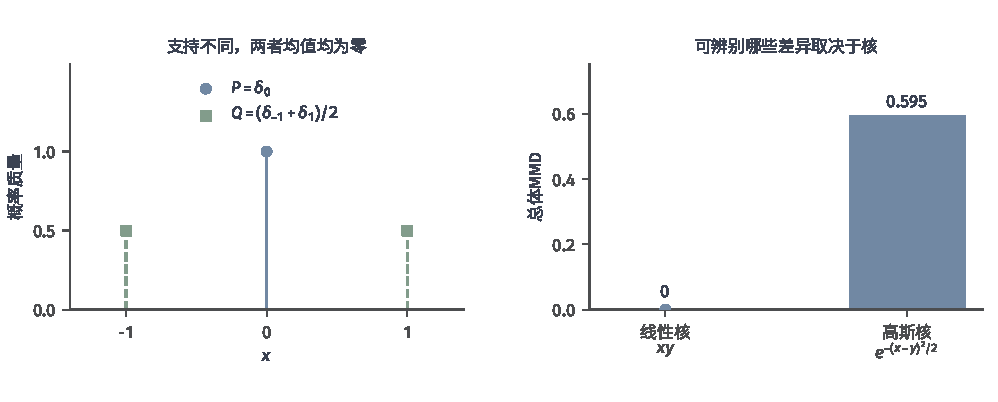
\includegraphics[width=\linewidth]{figures/02-mathematical-preliminaries-lower/01-random-variables-distributions-and-causality/matplotlib/information-kernel-distinguishability/figure.pdf}
  \caption{同均值分布在不同核下的MMD（解析式教学图）。左图为\(P=\delta_0\)与\(Q=(\delta_{-1}+\delta_1)/2\)，右图按精确总体期望计算：线性核给出零，高斯核给出约\(0.595\)。没有使用有限样本估计；差别来自测试函数类。}
  \label{fig:information-kernel-distinguishability}
\end{figure*}

\subsubsection{质量位置的差异}
\label{sec:information-optimal-transport}

两个不同位置上的点质量没有重叠，TV因而始终为一。若结果是温度读数，把全部质量移动\(0.01\)度与移动\(10\)度却有不同意义。事件概率差没有记录这两个位置之间的距离，质量位置的比较需要使用样本空间本身的几何。\term{最优传输}
（optimal transport, OT）寻找保持两边概率不变的最便宜配对
\scite{math-villani2009transport}

\begin{definition}[耦合]
\label{def:information-coupling}
给定\((\mathcal X,\mathcal A)\)、\((\mathcal Y,\mathcal B)\)上的概率测度\(P,Q\)，
其\term{耦合}（coupling）是乘积空间上的概率测度\(\gamma\)，满足
\[
  \gamma(A\times\mathcal Y)=P(A),\qquad
  \gamma(\mathcal X\times B)=Q(B).
\]
全体耦合记为\(\Pi(P,Q)\)。
\end{definition}
耦合规定一单位来源质量与哪部分目标质量配对，不改变两边总量。
独立耦合\(P\otimes Q\)总存在，但不一定便宜。
给定非负可测成本\(c(x,y)\)，Kantorovich搬运代价为
\begin{equation}
  \mathcal T_c(P,Q)=\inf_{\gamma\in\Pi(P,Q)}
                      \int c(x,y)\,\mathrm d\gamma(x,y).
  \label{eq:information-kantorovich-transport}
\end{equation}
下确界能否达到及怎样求解留到第~\ref{sec:information-coupling-optimization}节。
这里先把搬运用于比较分布。

\begin{definition}[Wasserstein距离]
\label{def:information-wasserstein-distance}
设\((\mathcal X,d)\)为完备可分度量空间，
\(1\leq r<\infty\)，固定基点\(x_0\)并令
\[
  \mathcal P_r(\mathcal X)=
   \left\{P:\int d(x,x_0)^r\,\mathrm dP(x)<\infty\right\}.
\]
对\(P,Q\in\mathcal P_r(\mathcal X)\)，定义
\begin{equation}
  W_r(P,Q)=\left[
    \inf_{\gamma\in\Pi(P,Q)}\int d(x,y)^r\,\mathrm d\gamma(x,y)
  \right]^{1/r}.
  \label{eq:information-wasserstein-distance}
\end{equation}
\end{definition}

由\(d(x,x_1)^r\leq2^{r-1}\{d(x,x_0)^r+d(x_0,x_1)^r\}\)，
矩条件不依赖基点；同一不等式说明独立耦合的成本有限。
对称性来自底层距离，对角耦合给出\(W_r(P,P)=0\)。
若\(W_r(P,Q)=0\)，任意有界\(L\)-Lipschitz函数的期望差至多
\(L(\mathbb E_\gamma d(X,Y)^r)^{1/r}\)，沿近最优耦合趋于零。
用连续函数\(\max\{1-kd(x,C),0\}\)逼近闭集\(C\)的指标，得到所有闭集上
\(P(C)=Q(C)\)，故\(P=Q\)。

要控制两个函数的乘积积分，先把\BookTheoremRef{thm:linear-algebra-holder}{卷1《数学准备：分析、几何与计算》第5章“线性空间”第5.2.3节“对象的距离关系”}的有限坐标配对
推广到函数积分。若\(1\leq p,q\leq\infty\)、\(1/p+1/q=1\)，且相应范数有限，则
\begin{equation}
 \int|uv|\,\mathrm d\mu\leq
 \|u\|_{L^p(\mu)}\|v\|_{L^q(\mu)}.
 \label{eq:information-integral-holder}
\end{equation}
这就是积分形式的Hölder不等式。对\(1<p,q<\infty\)，当两个范数非零时，
将\(|u|\)、\(|v|\)分别除以自己的范数，再逐点使用上述定理证明中的Young不等式并积分；
右侧归一化后为\(1/p+1/q=1\)，恢复尺度即得本式。
范数为零时相应函数几乎处处为零；端点\(p=1,q=\infty\)直接用
\(|v|\leq\|v\|_{L^\infty}\)几乎处处成立，另一端点交换两者。

三角不等式需要先控制随机距离之和。对\(u,v\in L^r(\mu)\)，这里使用Minkowski不等式
\(\|u+v\|_{L^r}\leq\|u\|_{L^r}+\|v\|_{L^r}\)。
它仍沿用有限维的证明：\(r=1\)直接对绝对值三角不等式积分；
\(1<r<\infty\)时，先由
\(|u+v|^r\leq2^{r-1}(|u|^r+|v|^r)\)确认\(u+v\in L^r\)，再写
\[
 \|u+v\|_{L^r}^r
 \leq\int|u+v|^{r-1}(|u|+|v|)\,\mathrm d\mu
 \leq\|u+v\|_{L^r}^{r-1}(\|u\|_{L^r}+\|v\|_{L^r}).
\]
末步对两项分别使用式~\eqref{eq:information-integral-holder}，指数为
\(r/(r-1)\)与\(r\)。非零时约去公共幂，零时结论直接成立。

还需把两个配对接起来。把\(P,Q\)的耦合分解为
\(P(\mathrm dx\mid y)Q(\mathrm dy)\)，把\(Q,R\)的耦合分解为
\(Q(\mathrm dy)R(\mathrm dz\mid y)\)。Polish空间上的正则条件分布允许构造
\[
  P(\mathrm dx\mid y)Q(\mathrm dy)R(\mathrm dz\mid y),
\]
其相邻边缘正是原来的两张耦合。这是粘合引理在这里的具体实现。
由\(d(X,Z)\leq d(X,Y)+d(Y,Z)\)及Minkowski不等式，
\[
  \bigl(\mathbb E d(X,Z)^r\bigr)^{1/r}
  \leq\bigl(\mathbb E d(X,Y)^r\bigr)^{1/r}
       +\bigl(\mathbb E d(Y,Z)^r\bigr)^{1/r}.
\]
分别选近最优耦合并令误差趋零，就得到\(W_r(P,R)\leq W_r(P,Q)+W_r(Q,R)\)。
一般成本\(c\)不具备这些距离性质，\(\mathcal T_c\)不能自动称为距离；
超出矩条件时，扩展定义还可能为无限。

对有限一阶矩的\(P,Q\)，Kantorovich--Rubinstein对偶给出
\begin{equation}
  W_1(P,Q)=\sup_{\operatorname{Lip}(f)\leq1}
                         |\mathbb E_Pf-\mathbb E_Qf|.
  \label{eq:information-kr-duality}
\end{equation}
其中\(\operatorname{Lip}(f)\leq1\)表示\(|f(x)-f(y)|\leq d(x,y)\)。
可以固定\(f(x_0)=0\)，不改变期望差，且一阶矩保证可积。
任意耦合都给出右侧不超过左侧；反向是最优传输对偶定理的实质内容，
这里按上述Polish及矩条件使用。有限空间的完整线性规划对偶将在后文推导。
这说明\(W_1\)也是IPM；\(r>1\)的\(W_r\)没有这里同一个Lipschitz单位球表达。

\subsubsection{对数评分的差异}
\label{sec:information-log-score-kl}

仍然编码结果，但接收者现在只持有预测分布\(Q\)，真实结果却来自\(P\)。
按\(Q\)分配的理想码长为\(-\log q(x)\)；高概率真实结果若被\(Q\)低估，
平均描述就会变长。\term{对数损失}（log loss）正是用这个代价评价概率预测。

\begin{definition}[离散交叉熵]
\label{def:information-cross-entropy}
对同一离散空间上的质量函数\(p,q\)，\term{交叉熵}（cross-entropy）定义为
\begin{equation}
  H(P,Q)=-\sum_xp(x)\log q(x).
  \label{eq:information-cross-entropy}
\end{equation}
零质量\(p(x)=0\)的项贡献为零；若\(p(x)>0\)而\(q(x)=0\)，则结果为\(+\infty\)。
\end{definition}

交叉熵不是\(Q\)自身的熵，因为平均所用的概率仍是\(P\)。
要分离无法消除的真实不确定性与预测失配，需要比较两个描述长度之差。
前章的Radon--Nikodym导数使这种比较不依赖离散或连续表示。

\begin{definition}[相对熵]
\label{def:information-kl-divergence}
同一可测空间上的概率测度\(P,Q\)若满足\(P\ll Q\)，令
\(L=\mathrm dP/\mathrm dQ\)。\term{相对熵}（relative entropy），也称KL散度，定义为
\begin{equation}
  D_{\mathrm{KL}}(P\Vert Q)
  =\int\log L\,\mathrm dP=\int L\log L\,\mathrm dQ.
  \label{eq:information-kl-divergence}
\end{equation}
若\(P\not\ll Q\)，约定为\(+\infty\)，并采用\(0\log0=0\)。
\end{definition}

负部积分总有限，因为在\(0\leq L\leq1\)上有
\(0\leq-L\log L\leq1/e\)。因此定义不会出现无穷减无穷；
有限性还要求正部可积，绝对连续本身并不足够。
在共同密度表示下，积分为\(\int p\log(p/q)\,\mathrm d\mu\)。
离散情形逐项分解得到
\begin{equation}
  H(P,Q)=H(P)+D_{\mathrm{KL}}(P\Vert Q).
  \label{eq:information-cross-entropy-decomposition}
\end{equation}
若\(H(P)<\infty\)，这说明真实分布固定时交叉熵的多余代价恰是KL。
若\(H(P)=+\infty\)，等式按扩展值理解，所有交叉熵都无限，不能再用它们比较候选，
但直接定义的KL仍可能有限。

\begin{theorem}[Gibbs不等式]
\label{thm:information-gibbs-inequality}
任意概率测度\(P,Q\)满足\(D_{\mathrm{KL}}(P\Vert Q)\geq0\)，
且等号当且仅当\(P=Q\)。
\end{theorem}
\begin{proof}
只需处理\(P\ll Q\)。取共同支配测度\(\mu=P+Q\)，密度为\(p,q\)，
在\(\{p>0\}\)上令\(r=q/p>0\)。由\(-\log r\geq1-r\)，
\[
  D_{\mathrm{KL}}(P\Vert Q)
  \geq1-\mathbb E_Pr
  =1-\int_{\{p>0\}}q\,\mathrm d\mu\geq0.
\]
等号要求非负差\(-\log r-1+r\)在\(P\)-几乎处处为零，即\(r=1\)，
并要求\(Q\)在\(\{p=0\}\)上没有额外质量，所以\(P=Q\)。
反过来\(P=Q\)时密度比为一，积分为零。
\end{proof}

在真实熵有限的离散分布类上，对数评分的期望只在真实分布处达到最小，
这称为严格适当性（strict propriety）：如实报告概率是总体期望最优的。
连续密度也可定义\(-\int p\log q\)并作同一分解，但必须先确认期望存在，
且真实密度的对数可积。有限样本的最小经验损失则是前章讨论的估计问题，
仍有模型限制、抽样偏差和求解误差，不能由适当性直接推断拟合正确。

KL的方向指定了谁来加权。取
\(P=\operatorname{Bernoulli}(0.9)\)、\(Q=\operatorname{Bernoulli}(0.6)\)，有
\[
  D_{\mathrm{KL}}(P\Vert Q)\approx0.2263,\qquad
  D_{\mathrm{KL}}(Q\Vert P)\approx0.3112.
\]
若\(Q(1)=0<P(1)\)，前向KL无限；反向是否有限仍需检查反向支持。
它也不是满足三角不等式的距离。令\(P,Q,R\)依次为参数
\(0.1,0.2,0.3\)的Bernoulli分布，则
\[
  D_{\mathrm{KL}}(P\Vert R)\approx0.1163
  >D_{\mathrm{KL}}(P\Vert Q)+D_{\mathrm{KL}}(Q\Vert R)
  \approx0.0624.
\]

对\(P=\mathcal N(\mu,\sigma^2)\)、\(Q=\mathcal N(\nu,\sigma^2)\)，
\(\sigma>0\)，对数密度比为
\(\{(x-\nu)^2-(x-\mu)^2\}/(2\sigma^2)\)。
按\(P\)平均时交叉项均值为零，故
\begin{equation}
  D_{\mathrm{KL}}(P\Vert Q)=\frac{(\mu-\nu)^2}{2\sigma^2}.
  \label{eq:information-gaussian-location-kl}
\end{equation}
同样，对共同正定协方差\(\bm\Sigma\)的向量高斯，
\begin{equation}
  D_{\mathrm{KL}}\bigl(
    \mathcal N(\bm\mu,\bm\Sigma)\Vert\mathcal N(\bm\nu,\bm\Sigma)\bigr)
  =\tfrac12(\bm\mu-\bm\nu)^\top\bm\Sigma^{-1}(\bm\mu-\bm\nu).
  \label{eq:information-vector-gaussian-translation-kl}
\end{equation}
这比较白化后的均值移动：沿低方差方向的同样位移更容易辨认。
若\(\bm\Sigma\)只半正定，两个仿射支持相同当且仅当
\(\bm\mu-\bm\nu\in\operatorname{range}(\bm\Sigma)\)。
支持相同时可限制到该子空间并使用\(\bm\Sigma^\dagger\)；
否则两支持不相交，KL无限。不能只替换成伪逆而忽略支持条件。

若对\(P,Q\)同时施加可测双射\(g\)，且逆映射可测，则推送密度比为
\(L\circ g^{-1}\)，所以KL保持不变。光滑换元时，这就是两个Jacobian项相消。
非可逆处理通常会丢失差异。若通过共同概率核\(K\)输出\(Y\)，在联合参考规律
\(Q(\mathrm dx)K(\mathrm dy\mid x)\)下有
\[
  \frac{\mathrm d(PK)}{\mathrm d(QK)}(Y)=\mathbb E_Q[L(X)\mid Y].
\]
由\(u\log u\)的凸性和条件Jensen不等式，
\[
  D_{\mathrm{KL}}(PK\Vert QK)
  \leq\mathbb E_Q[L\log L]=D_{\mathrm{KL}}(P\Vert Q).
\]
这在扩展值意义下成立；不绝对连续时右侧无限，界仍成立。
核可以是确定映射，也可以使用额外随机性，但必须对两个输入规律采用同一处理规则。

\par\medskip
概率权重差异与对数评分差异已经分别定义，现在可以比较两种尺度。下面的Pinsker界把有限KL转成事件概率的统一控制；更高阶密度比的矩则约束罕见事件的概率放大。这些结论都保留绝对连续的方向，不能把一个单向界当作对称距离。

\begin{theorem}[Pinsker不等式]
\label{thm:information-pinsker}
以自然对数定义KL时，
\begin{equation}
  d_{\mathrm{TV}}(P,Q)\leq
  \sqrt{\tfrac12D_{\mathrm{KL}}(P\Vert Q)}.
  \label{eq:information-pinsker}
\end{equation}
\end{theorem}
\begin{proof}
KL无限时无需证明；否则\(P\ll Q\)。令
\(A=\{\mathrm dP/\mathrm dQ\geq1\}\)、\(a=P(A)\)、\(b=Q(A)\)，
则\(a-b=d_{\mathrm{TV}}(P,Q)\)。
在\(A\)及其补集分别对密度比使用条件Jensen不等式，得到
\[
  D_{\mathrm{KL}}(P\Vert Q)\geq
  a\log\frac ab+(1-a)\log\frac{1-a}{1-b}.
\]
固定\(b\in(0,1)\)，右侧作为\(a\)的函数在\(a=b\)处值和一阶导数为零，
二阶导数为\(1/[a(1-a)]\geq4\)。Taylor积分余项给出至少\(2(a-b)^2\)。
端点通过连续延拓处理；若\(b=0\)或\(1\)，有限KL迫使相应\(a=b\)。
整理即得结论。
\end{proof}

取\(P=\operatorname{Bernoulli}(1/4)\)、\(Q=\operatorname{Bernoulli}(1/2)\)，
则
\[
  d_{\mathrm{TV}}=\tfrac14,\qquad
  d_{\mathrm H}^2\approx0.0341,\qquad
  D_{\mathrm{KL}}(P\Vert Q)\approx0.1308.
\]
Pinsker给出的上界约为\(0.2557\)。这个控制不能反用：
\(P=(1-\eta)\delta_0+\eta\delta_1\)、\(Q=\delta_0\)的总变差只有\(\eta\)，
但只要\(\eta>0\)，前向KL就无限。

KL平均对数密度比；如果要限制极端密度比给事件概率带来的放大，
则可以直接控制更高阶矩。

\begin{definition}[高于一阶的Rényi散度]
\label{def:information-renyi-divergence}
对\(\alpha>1\)及\(P\ll Q\)，\term{R\'enyi散度}定义为
\begin{equation}
  D_\alpha(P\Vert Q)
   =\frac1{\alpha-1}\log\mathbb E_Q
       \left[\left(\frac{\mathrm dP}{\mathrm dQ}\right)^\alpha\right].
  \label{eq:information-renyi-divergence}
\end{equation}
若绝对连续性失败或该阶矩无限，结果为\(+\infty\)。
\end{definition}

令\(L=\mathrm dP/\mathrm dQ\)，Jensen给出
\(\mathbb E_Q L^\alpha\geq(\mathbb E_QL)^\alpha=1\)，故散度非负。
比较不同阶数时，回用式~\eqref{eq:information-integral-holder}的积分配对界。
取有限矩对应的\(a,b\geq1\)与\(0<t<1\)，对
\(u=L^{ta}\)、\(v=L^{(1-t)b}\)使用指数\(p=1/t\)、\(q=1/(1-t)\)，得到
\[
 \mathbb E_Q L^{ta+(1-t)b}
 \leq(\mathbb E_Q L^a)^t(\mathbb E_Q L^b)^{1-t}.
\]
取对数便说明\(K(\alpha)=\log\mathbb E_QL^\alpha\)在有限区间上为凸函数；
连同无穷值约定，它是扩展实值凸函数。
又因\(K(1)=0\)，割线斜率\(K(\alpha)/(\alpha-1)\)随阶数不减。
若某个\(\alpha_0>1\)的阶矩有限，则从右侧趋于一时可对矩函数求导，
得到\(D_\alpha\to\mathbb E_Q L\log L=D_{\mathrm{KL}}\)。
更大的阶数更强调大密度比，而不是更大的空间位移。
对上述Bernoulli例，\(\mathbb E_QL^2=1.25\)，
所以\(D_2=\log1.25\approx0.2231\)，高于KL。
事件迁移将在第~\ref{sec:information-bounded-evaluation}节使用这一阶矩；
重复机制的组合需要另外检查独立性或条件界。

\paragraph{同一位置变化下的差异尺度}
用同方差高斯来比较三种尺度。令\(P=\mathcal N(\mu,\sigma^2)\)、
\(Q=\mathcal N(\nu,\sigma^2)\)。取\(Y=X+\nu-\mu\)得到恒定位移耦合，
而任意耦合满足
\(\mathbb E|X-Y|^2\geq|\mathbb EX-\mathbb EY|^2=|\mu-\nu|^2\)，故
\begin{equation}
  W_2(P,Q)=|\mu-\nu|.
  \label{eq:information-gaussian-location-wasserstein}
\end{equation}
若\(\mu<\nu\)，两密度在\(c=(\mu+\nu)/2\)相交，
\(P\)在\((-\infty,c]\)上的密度较大。因此
\[
  d_{\mathrm{TV}}(P,Q)
  =P((-\infty,c])-Q((-\infty,c])
  =2\Phi\left(\frac{|\mu-\nu|}{2\sigma}\right)-1.
\]
当\(|\mu-\nu|=0.2,\sigma=1\)时，\(W_2=0.2\)、KL为\(0.02\)、
TV约为\(0.0797\)。若标准差\(\sigma\)减半，搬运位移不变，KL增为\(0.08\)，TV也增大。
位置差与可辨别程度因此不能互换。

图~\ref{fig:information-gaussian-distances}保留同一位置族的三尺度对照，
面板纵轴不同，不能按曲线高度判断哪一种概念更强。
\begin{figure*}[htbp]
  \centering
  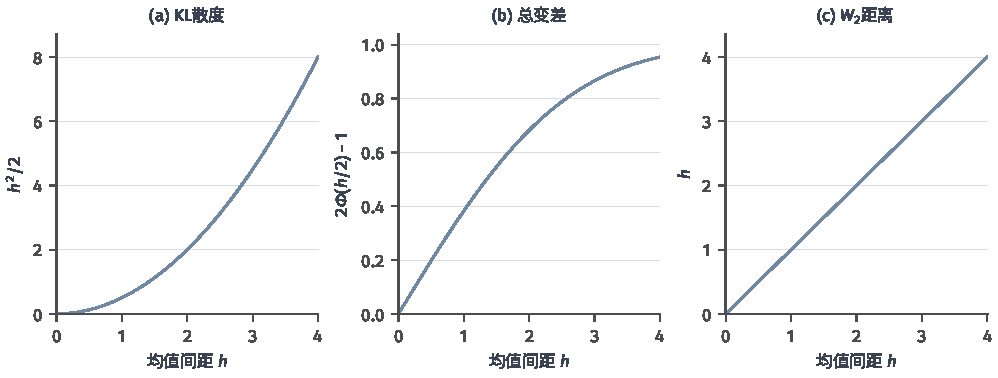
\includegraphics[width=\linewidth]{figures/02-mathematical-preliminaries-lower/01-random-variables-distributions-and-causality/matplotlib/information-gaussian-distances/figure.pdf}
  \caption{同方差高斯位置族的解析式比较。固定\(P=\mathcal N(0,1)\)、\(Q=\mathcal N(h,1)\)，三图分别为\(D_{\mathrm{KL}}=h^2/2\)、\(d_{\mathrm{TV}}=2\Phi(h/2)-1\)与\(W_2=h\)，图中\(h\geq0\)。纵轴分别表达对数代价、事件概率差与搬运位移。}
  \label{fig:information-gaussian-distances}
\end{figure*}

对点质量\(\delta_0,\delta_\varepsilon\)，只要\(\varepsilon\neq0\)，
TV恒为一、两个方向KL均无限，而\(W_r=|\varepsilon|\to0\)。
这是支持移动在不同尺度下的极限差别。
对时间边缘分布\((P_t)\)也可比较这些距离，但它们不决定轨迹机制：
每时刻都为同一公平二元分布，既可能来自反复独立抽样，也可能来自把初次抽样永远复制。
两过程边缘距离为零，时间依赖却完全不同，必须比较联合轨迹。
实际估计MMD或Wasserstein还需考虑核、底层成本、矩和样本量；
高维经验搬运的估计误差可能很大，精确总体公式不自动给出便宜的样本估计。

\subsection{联合分布的依赖关系}
\label{sec:information-mutual-relations}

现有差异工具还可以用于两个变量之间的关系。固定它们的真实联合分布，再用各自边缘的独立乘积作参照：两张分布有相同的单变量边缘，差异只来自共同变化。以KL比较这两个对象，便得到互信息，衡量联合规律对独立规律的偏离。

\subsubsection{无条件下的依赖关系}
\label{sec:information-unconditional-mi}

\begin{definition}[互信息]
\label{def:information-mutual-information}
对具有联合分布\(P_{XY}\)的随机元素\(X,Y\)，\term{互信息}
（mutual information, MI）定义为
\begin{equation}
  I(X;Y)=D_{\mathrm{KL}}(P_{XY}\Vert P_X\otimes P_Y).
  \label{eq:information-mutual-information}
\end{equation}
定义适用于一般可测空间，允许值为\(+\infty\)，不要求先存在密度或有限熵。
\end{definition}

Gibbs不等式给出非负性，而且\(I(X;Y)=0\)当且仅当\(X,Y\)独立。
这强于零协方差：例如\(X\)在\(\{-1,0,1\}\)上均匀，\(Y=X^2\)，
协方差为零，但\(Y\)完全由\(X\)确定，互信息为
\(H(Y)=H_{\mathrm b}(1/3)>0\)。
对可数离散变量，定义展开为
\(\sum_{x,y}p(x,y)\log[p(x,y)/(p(x)p(y))]\)；
当\(H(X,Y)<\infty\)时，展开对数并用熵链式法则可得
\begin{equation}
  I(X;Y)=H(X)-H(X\mid Y)=H(Y)-H(Y\mid X).
  \label{eq:information-mi-entropy-reduction}
\end{equation}
所以互信息是观测平均消除的不确定性。连续变量在相关微分熵均有限时也可作相应分解，
但KL定义更一般。例如连续的\(Y=X\)可能使联合分布落在对角线上，
相对于边缘乘积奇异，此时互信息无限，不能强行用有限密度公式计算。

回到例~\ref{ex:information-binary-channel}，有
\(I(X;Y)=\log2-H_{\mathrm b}(\varepsilon)\)。
图~\ref{fig:information-binary-channel-information}中两条曲线相加始终为\(\log2\)；
翻转噪声改变的是观测可提供的信息，而不是公平输入自身的熵。
\begin{figure}[htbp]
  \centering
  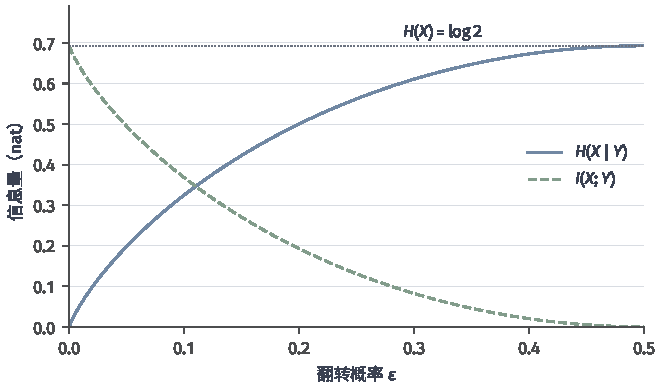
\includegraphics[width=\linewidth]{figures/02-mathematical-preliminaries-lower/01-random-variables-distributions-and-causality/matplotlib/information-binary-channel-information/figure.pdf}
  \caption{公平二元输入通过独立翻转通道后的信息分配（解析式教学图）。蓝实线为剩余条件熵\(H_{\mathrm b}(\varepsilon)\)，绿虚线为互信息\(\log2-H_{\mathrm b}(\varepsilon)\)，均以nat计。输入熵保持不变，零噪声与公平翻转分别对应完整信息与零信息。}
  \label{fig:information-binary-channel-information}
\end{figure}
由于对两个变量分别施加可逆变换会同时推送联合分布与边缘乘积，
互信息继承KL的不变性。这与微分熵随坐标单位改变形成区别。

\subsubsection{条件观测下的依赖关系}
\label{sec:information-conditional-mi}

已经知道\(Z\)时，应在同一个条件值下判断\(X,Y\)是否还有关系，
再按\(Z\)的发生概率平均。不能把三者的边缘依赖随意相减。

\begin{definition}[条件互信息]
\label{def:information-conditional-mi}
设\(X,Y,Z\)取值于标准Borel空间，因而存在所需正则条件分布。
\term{条件互信息}（conditional mutual information）定义为
\begin{equation}
  I(X;Y\mid Z)
  =\int D_{\mathrm{KL}}\bigl(
    P_{XY\mid z}\Vert P_{X\mid z}\otimes P_{Y\mid z}\bigr)\,P_Z(\mathrm dz).
  \label{eq:information-conditional-mutual-information}
\end{equation}
条件核的版本只需在\(P_Z\)-几乎处处确定；被积量非负，允许结果为\(+\infty\)。
\end{definition}

在不保证正则条件分布存在的一般空间上，不能不加条件地沿用这个条件核定义。
在上述条件下，零条件互信息等价于条件联合核几乎处处等于条件边缘乘积，
也就是前章的条件独立。有限熵时可写成
\(H(X\mid Z)-H(X\mid Y,Z)\)，但非负KL积分是避免无穷相减的基本口径。

条件化并不一定使互信息变小。取独立公平二元变量\(X,Y\)，令\(Z=X\oplus Y\)。
边缘上互信息为零；固定\(Z\)后，\(X\)完全决定\(Y\)，条件互信息为\(\log2\)。
反过来，若\(X=Y=Z\)为同一个公平二元变量，无条件互信息为\(\log2\)，
条件互信息却为零。前者揭示约束，后者去掉已经知道的共享信息。

后处理和序贯观测都要用到KL的条件分解。设联合规律满足\(P_{AB}\ll Q_{AB}\)，并存在所需正则条件核。
这推出\(P_A\ll Q_A\)，以及在\(P_A\)-几乎处处的条件值上
\(P_{B\mid A}\ll Q_{B\mid A}\)。联合密度比分解为边缘比与条件比的乘积，
取对数并用塔式性质得到
\begin{equation}
  D_{\mathrm{KL}}(P_{AB}\Vert Q_{AB})
  =D_{\mathrm{KL}}(P_A\Vert Q_A)
   +\mathbb E_{A\sim P_A}
       D_{\mathrm{KL}}(P_{B\mid A}\Vert Q_{B\mid A}).
  \label{eq:information-kl-conditional-chain}
\end{equation}
每个对数比的负部可积，故有限项相加的分解也能按非负扩展值成立；
若绝对连续性失败，对应的条件或边缘项为无限。
把\(Q_{XYZ}\)选为\(P_X\otimes P_{YZ}\)，再按\((X,Y)\)与\(Z\)分组，
第一项是\(I(X;Y)\)，条件项是
\(\mathbb E_{X,Y}D_{\mathrm{KL}}(P_{Z\mid X,Y}\Vert P_{Z\mid Y})
=I(X;Z\mid Y)\)。因此
\[
  I(X;Y,Z)=I(X;Y)+I(X;Z\mid Y).
\]
这证明了互信息链式法则，而不仅是引用熵差记号。

\begin{theorem}[数据处理不等式]
\label{thm:information-data-processing}
若标准Borel随机元素满足Markov关系\(X\to Y\to Z\)，
即\(X\perp Z\mid Y\)，则\(I(X;Z)\leq I(X;Y)\)，允许扩展值。
\end{theorem}
\begin{proof}
用两种顺序分解同一联合信息量：
\[
\begin{aligned}
  I(X;Y,Z)&=I(X;Y)+I(X;Z\mid Y)=I(X;Y),\\
  I(X;Y,Z)&=I(X;Z)+I(X;Y\mid Z)\geq I(X;Z).
\end{aligned}
\]
第一行的条件项由条件独立为零，第二行的条件项非负，合并即得。
证明只作非负项的相加和比较，不需要有限熵，也没有无穷相减。
\end{proof}

处理可以是\(Z=g(Y)\)，也可以是仅依赖\(Y\)的随机通道。
若额外随机性还与\(X\)关联，Markov前提可能不成立。
信息不增加并不保证每个任务的误差严格增加；当丢弃的内容与任务无关时可以取等号。

\section{基于观测的分布区分}
\label{sec:information-lower-bounds}

若两套候选规律产生很相近的观测分布，却对应相距较远的目标值，那么程序很难从记录辨认目标属于哪套规律。前面的分布差异现在成为辨认难度的依据。我们固定候选总体、目标及可用观测，对所有估计程序的错误给出下界；这个下界来自信息不足，不依赖某个特定算法的实现。

\subsection{固定观测下的分布区分}
\label{sec:information-fixed-observations}

先把整批观测的分布视为已给定，不让程序根据中途结果改变取样位置。
两候选比较利用TV，多候选比较则需要把候选数量也纳入信息预算。

\paragraph{两个候选的区分下界}
\label{sec:information-two-candidates}

设观测\(Z\)来自\(P_0\)或\(P_1\)，先验各为\(1/2\)。
检验\(\psi(Z)\in\{0,1\}\)以事件\(A=\{\psi=1\}\)选择第二个候选，则错误和为
\[
  P_0(A)+P_1(A^{\mathsf c})=1-\{P_1(A)-P_0(A)\}.
\]
取使密度差为正的事件达到上确界，得到
\begin{equation}
  \inf_\psi\{P_0(\psi=1)+P_1(\psi=0)\}
     =1-d_{\mathrm{TV}}(P_0,P_1).
  \label{eq:information-binary-testing-tv}
\end{equation}
随机化检验只是把指标改为\([0,1]\)值函数，按TV的函数表达也不能降低这个值。
在等先验下，最小总体错误是右侧的一半；两类条件错误之和本身不是总体错误。

数值估计可以转成检验：若估计足够准，就应能知道它靠近哪个候选目标。

\begin{theorem}[Le Cam两点下界]
\label{thm:information-le-cam}
设观测模型\(P_0,P_1\)对应目标\(\theta_0,\theta_1\)，
在目标空间度量\(d\)下有\(d(\theta_0,\theta_1)\geq2s\)，\(s>0\)。
任意估计量\(\widehat\theta\)均满足
\begin{equation}
  \max_{j\in\{0,1\}}P_j\{d(\widehat\theta,\theta_j)\geq s\}
  \geq\frac{1-d_{\mathrm{TV}}(P_0,P_1)}2.
  \label{eq:information-le-cam}
\end{equation}
\end{theorem}
\begin{proof}
构造最近目标检验
\(\psi=\mathbb I\{d(\widehat\theta,\theta_1)<d(\widehat\theta,\theta_0)\}\)，
距离相等时选\(0\)。若真实为\(0\)且估计误差小于\(s\)，由三角不等式，
估计与\(\theta_1\)的距离大于\(s\)，检验不会错。
真实为\(1\)时同理。因此检验错误分别包含在估计坏事件内。
两个坏事件概率之和至少为\(1-d_{\mathrm{TV}}(P_0,P_1)\)，
其中最大者至少为一半，即得结论。
\end{proof}

若每个候选下都得到\(n\)个独立同分布观测，联合密度比是单次密度比的乘积，
取对数并平均得到
\(D_{\mathrm{KL}}(P_0^{\otimes n}\Vert P_1^{\otimes n})
=nD_{\mathrm{KL}}(P_0\Vert P_1)\)。
取单次规律为\(\mathcal N(-a,\sigma^2)\)与\(\mathcal N(a,\sigma^2)\)，
目标均值相距\(2a\)，整批KL为\(2na^2/\sigma^2\)。
令\(a=\sigma/(2\sqrt n)\)，KL为\(1/2\)，Pinsker给出TV至多\(1/2\)。
所以任何均值估计量都至少在一个候选下，以不小于\(1/4\)的概率产生
不小于\(\sigma/(2\sqrt n)\)的绝对误差。
若评价平方误差，还可由这个事件下界得到最坏风险至少\(\sigma^2/(16n)\)。
这些常数来自所选两点及放缩，不声称最优。

\paragraph{多个候选的区分下界}
\label{sec:information-many-candidates}

两点只要求区分一个二元选择；高维问题可能同时包含许多不同目标。
令\(V\)在\(\{1,\ldots,M\}\)上均匀，给定\(V=v\)后观测\(Z\sim P_v\)。
解码器\(\widehat V(Z)\)的错误概率记为\(p_{\mathrm e}\)。
即使\(Z\)连续，\(V\)的条件熵仍可按其有限后验概率求熵，再对\(Z\)积分。

\begin{theorem}[Fano不等式]
\label{thm:information-fano}
对\(M\geq2\)及上述观测模型，
\begin{equation}
  p_{\mathrm e}\geq1-\frac{I(V;Z)+\log2}{\log M}.
  \label{eq:information-fano}
\end{equation}
\end{theorem}
\begin{proof}
令\(E=\mathbb I\{\widehat V\neq V\}\)。给定\(Z\)且\(E=0\)时，
\(V=\widehat V(Z)\)已确定；给定\(E=1\)时，至多还有\(M-1\)个可能索引。
有限字母表上最大熵为均匀熵，这也可由与均匀分布的Gibbs不等式得到。
于是
\[
\begin{aligned}
  H(V\mid Z)
  &\leq H(V,E\mid Z)\\
  &=H(E\mid Z)+H(V\mid E,Z)\\
  &\leq\log2+p_{\mathrm e}\log(M-1)
   \leq\log2+p_{\mathrm e}\log M.
\end{aligned}
\]
又因\(H(V)=\log M\)，互信息分解给出
\(H(V\mid Z)=\log M-I(V;Z)\)。移项得到结论。
随机化解码可把独立随机种子并入\(Z\)，不会增加关于\(V\)的信息。
\end{proof}

若目标集合中有两两距离至少\(2s\)的有限分离集
\(\{\theta_1,\ldots,\theta_M\}\)，误差小于\(s\)就能最近邻解码。
这把前面计数与打包的工具接到统计下界：候选多能提高\(\log M\)，
但必须同时控制观测中含有多少索引信息\scite{math-cover2006information}
令\(\overline P=M^{-1}\sum_uP_u\)，则
\[
  I(V;Z)=\frac1M\sum_vD_{\mathrm{KL}}(P_v\Vert\overline P)
  \leq\frac1{M^2}\sum_{v,u}D_{\mathrm{KL}}(P_v\Vert P_u).
\]
等式来自给定\(V\)的条件KL分解；不等式来自
\(-\log(M^{-1}\sum_u p_u)\leq M^{-1}\sum_u(-\log p_u)\)。
因此
\(\max_vP_v\{d(\widehat\theta,\theta_v)\geq s\}\)
至少为Fano右侧，若右侧为负则只得到平凡下界零。

保留一个可复算的四候选构造：均值为\(\{-3a,-a,a,3a\}\)，
每个候选产生\(n\)个方差\(\sigma^2\)的独立高斯观测。
最小间距为\(2a\)，有序候选对的平均平方距离为\(10a^2\)，故
\[
  I(V;Z)\leq\frac{5na^2}{\sigma^2}.
\]
取\(a=\sigma/(4\sqrt n)\)时右侧为\(5/16\)，Fano给出
\(p_{\mathrm e}\geq1-(5/16+\log2)/\log4\approx0.2746\)。
任意估计器因此至少在一个候选上以这一概率产生不小于\(a\)的误差。
目标分离与观测接近必须同时成立；只罗列许多模型不构成下界证明。

\subsection{序贯观测下的分布区分}
\label{sec:information-sequential-observations}

若观测位置根据已获得的结果改变，最终资料的联合分布也随算法改变。
仍可使用前面的检验不等式，但比较对象应当是包含行动与结果的完整轨迹。

\paragraph{重复与时序观测的信息累积}
\label{sec:information-sequential-accumulation}

独立重复是简单情形。固定有限个分量\(t=1,\ldots,T\)，假设\(P_t\ll Q_t\)，密度比为\(L_t\)。
乘积规律的比值为\(\prod_tL_t\)，因此
\[
\begin{aligned}
  D_{\mathrm{KL}}\left(\bigotimes_tP_t\Big\Vert\bigotimes_tQ_t\right)
     &=\sum_tD_{\mathrm{KL}}(P_t\Vert Q_t),\\
  D_\alpha\left(\bigotimes_tP_t\Big\Vert\bigotimes_tQ_t\right)
     &=\sum_tD_\alpha(P_t\Vert Q_t),\qquad\alpha>1.
\end{aligned}
\]
第一式由对数把乘积化为和；第二式由独立性使
\(\mathbb E_{\otimes Q_t}\prod_tL_t^\alpha=\prod_t\mathbb E_{Q_t}L_t^\alpha\)。
公式可按扩展值理解，不通过相减处理无限项。

一般序列不独立。设\(Z_{0:T}\)在标准Borel空间取值，两个规律分解为初始分布及
历史条件核，\(P_0\ll Q_0\)，且在相关的\(P\)-历史上
\(P_t(\cdot\mid Z_{<t})\ll Q_t(\cdot\mid Z_{<t})\)。
前章条件换测度给出联合密度比
\[
  L_{0:T}=L_0(Z_0)\prod_{t=1}^T L_t(Z_t\mid Z_{<t}).
\]
对数相加，再对每一项先按历史条件平均，得到
\begin{equation}
\begin{aligned}
 D_{\mathrm{KL}}(P_{0:T}\Vert Q_{0:T})
 &=D_{\mathrm{KL}}(P_0\Vert Q_0)\\
 &\quad+\sum_{t=1}^T\mathbb E_{Z_{<t}\sim P}
 D_{\mathrm{KL}}\bigl(P_t(\cdot\mid Z_{<t})
                     \Vert Q_t(\cdot\mid Z_{<t})\bigr).
\end{aligned}
\label{eq:information-trajectory-kl-chain}
\end{equation}
这是式~\eqref{eq:information-kl-conditional-chain}的反复应用。
有限时域中每个条件对数比的负部积分均有统一有限界，
故可合法按扩展值累加；得到有限数值则还需累计条件KL有限。
期望必须沿前向分布\(P\)实际产生的历史计算。

轨迹包含行动时，同一算法在同一历史上使用相同的条件行动核，
所以比较两个环境时行动因子相消；两个环境的历史频率却不会相消。
在同一环境比较两条策略时，则是环境核相消，剩下条件行动KL。
若两者都改变，不能省略其中任何一组项。

Rényi不能把条件散度直接按\(P\)平均。一个充分组合条件是：在\(Q\)-几乎处处的历史上，
\(P_t(\cdot\mid h_{<t})\ll Q_t(\cdot\mid h_{<t})\)，并且有确定的统一界
\[
  D_\alpha(P_t(\cdot\mid h_{<t})\Vert Q_t(\cdot\mid h_{<t}))
  \leq\varepsilon_t.
\]
为简化记号从\(t=1\)开始且初始历史固定。在\(Q\)下从最后一步取条件期望，
\[
  \mathbb E_Q[L_t^\alpha\mid h_{<t}]
       \leq e^{(\alpha-1)\varepsilon_t}.
\]
前面的密度比是历史可测量，因此每消去一步至多乘上这个常数。
反复迭代后
\[
  \mathbb E_Q L_{1:T}^{\alpha}
  \leq e^{(\alpha-1)\sum_t\varepsilon_t},\qquad
  D_\alpha(P_{1:T}\Vert Q_{1:T})\leq\sum_t\varepsilon_t.
\]
若只在某种历史分布下给出平均条件界，后续选择可能偏向高散度历史，
不能据此使用这个组合结论。

固定有限时域无需停止论证。若共同停止规则给出\(\tau\leq T\)，
停止后补同一个吸收符号，其条件信息代价为零，公式仍适用。
无界停时则应确认在所比较的规律下几乎处处终止；
一种足够的取极限条件是截断累计对数似然比
\(\log L_{0:\tau\wedge n}\)在\(P\)下均匀可积并收敛到停止轨迹的对数密度比。
此时左侧期望可取极限，右侧的非负条件KL用单调收敛。
终止本身不能代替这些可积条件。
隐私分析若使用组合式，还必须另外规定相邻输入、随机机制，
以及对全部相邻输入统一成立的界；单个分布对的散度不是完整隐私定义。

\paragraph{自适应观测的区分下界}
\label{sec:information-adaptive-lower-bounds}

固定有限时域\(T\)，设算法\(\mathcal A\)在时刻\(t\)根据历史，
从有限或可数位置集合中选择来源或状态行动对\((s,a)\)。
观测取值于标准Borel空间，在环境\(j\)中的核为\(P_j(\cdot\mid s,a)\)，
并假设每个允许位置上都有\(P_0(\cdot\mid s,a)\ll P_1(\cdot\mid s,a)\)。
若初始规律相同、条件行动规则相同，且观测在给定历史及当前\((s,a)\)后使用该核，
轨迹链式法则可按访问位置分组：
\[
  D_{\mathrm{KL}}(\mathbb P_0^{\mathcal A}\Vert\mathbb P_1^{\mathcal A})
  =\sum_{s,a}\mathbb E_0N_T(s,a)\,
      D_{\mathrm{KL}}(P_0(\cdot\mid s,a)\Vert P_1(\cdot\mid s,a)).
\]
这里\(N_T(s,a)\)为\(T\)步中的访问次数；等式来自
\(\sum_t\mathbb I\{(S_t,A_t)=(s,a)\}=N_T(s,a)\)。
当某位置的期望访问次数为零时，该项约定为零，即使位置核的KL为无限。
访问次数是由算法和环境共同产生的随机量，不能预先替换成均匀独立的样本数。
连续位置不能用点访问次数的可数求和表示；此时应保留式~\eqref{eq:information-trajectory-kl-chain}
中的逐时条件期望，或对期望访问测度积分。
核若还依赖其他历史，保留逐步条件KL形式，不能强行按固定位置常数提取。

考虑两个可选Bernoulli来源\(A,B\)。环境\(0\)的均值为
\((1/2+\varepsilon,1/2)\)，环境\(1\)为
\((1/2+\varepsilon,1/2+2\varepsilon)\)，\(0<\varepsilon<1/4\)。
每次访问给出独立于过去的相应来源新观测，但来源选择允许自适应。
两个环境的最优来源相反，全部区分信息只来自\(B\)，单次KL为
\[
  \kappa(\varepsilon)
  =D_{\mathrm{KL}}\bigl(\operatorname{Bernoulli}(1/2)
             \Vert\operatorname{Bernoulli}(1/2+2\varepsilon)\bigr)
  =-\tfrac12\log(1-16\varepsilon^2).
\]
故轨迹KL为\(\mathbb E_0N_T(B)\kappa(\varepsilon)\)。
若输出的来源在两个环境下的错误都不超过\(\delta<1/2\)，
检验恒等式迫使TV至少为\(1-2\delta\)，Pinsker进一步给出
\[
  \mathbb E_0N_T(B)\geq
  \frac{2(1-2\delta)^2}{\kappa(\varepsilon)}.
\]
例如\(\varepsilon=0.1,\delta=0.1\)，有
\(\kappa\approx0.08718\)，期望访问至少约\(14.68\)次。
当\(\varepsilon\)小时，\(\kappa=8\varepsilon^2+O(\varepsilon^4)\)，
因此固定错误水平需要\(\varepsilon^{-2}\)量级的区分观测。
这是信息不足的预算下界，不是某个算法已达到该预算的上界。
推广到无界停止必须满足上一段的终止和可积条件；
更具体的价值或累计决策损失还要引入相应任务定义。

\section{概率分布变化下的期望响应}
\label{sec:information-task-stability}
\label{sec:information-fixed-evaluation}

同一个评价函数在两张分布下有两个期望，我们现在要控制它们的差。若函数取值有界，事件概率差足以给出控制；若函数随位置变化缓慢，可以利用搬运距离；若参考分布能控制函数尾部，则可结合指数矩与KL。以下分别改变已知条件，函数本身和所比较的两张分布仍要明确固定。

\subsection{有界函数的期望响应}
\label{sec:information-bounded-evaluation}

设固定可测损失\(f\)取值于\([0,1]\)。逐点恒等式
\(f(x)=\int_0^1\mathbb I\{f(x)>t\}\,\mathrm dt\)与Tonelli定理给出
\[
  |\mathbb E_Pf-\mathbb E_Qf|
  \leq\int_0^1|P(f>t)-Q(f>t)|\,\mathrm dt
  \leq d_{\mathrm{TV}}(P,Q).
\]
这也说明事件概率控制为何足以控制所有这一范围内的损失。
若\(a<b\)且\(a\leq f\leq b\)，对\((f-a)/(b-a)\)使用同一式子，得到
\[
  |\mathbb E_Pf-\mathbb E_Qf|
  \leq(b-a)d_{\mathrm{TV}}(P,Q).
\]
若\(a=b\)，函数为常量，两侧期望差为零，这个上界仍成立。
特别地，\(|f|\leq1\)时常数是\(2\)，不能把它与\(0\leq f\leq1\)混用。
取两点上的\(P=\delta_0,Q=\delta_1\)和\(f(0)=-1,f(1)=1\)，
期望差为\(2\)，已经表明这个因子不能删除。
在\(a<b\)时结合Pinsker，还可用\((b-a)\sqrt{D_{\mathrm{KL}}(P\Vert Q)/2}\)控制期望差；
若KL无限，这个途径不给出有限信息，但TV界仍有效。

对罕见失败事件，除了TV的加性误差，还可以利用似然比高阶矩。
设\(P\ll Q\)、\(L=\mathrm dP/\mathrm dQ\)，并且某个\(\alpha>1\)满足
\(D_\alpha(P\Vert Q)<\infty\)。由H\"older不等式，
\[
  P(A)=\mathbb E_Q[L\mathbb I_A]
  \leq(\mathbb E_QL^\alpha)^{1/\alpha}
       (\mathbb E_Q\mathbb I_A^{\alpha/(\alpha-1)})^{(\alpha-1)/\alpha}.
\]
代入R\'enyi散度定义，得到
\begin{equation}
  P(A)\leq
  \exp\!\left\{\frac{\alpha-1}{\alpha}D_\alpha(P\Vert Q)\right\}
  Q(A)^{(\alpha-1)/\alpha}.
  \label{eq:information-renyi-event-bound}
\end{equation}
若\(Q(A)=0\)，绝对连续直接给出\(P(A)=0\)，无需计算无穷与零的乘积。
若\(Q(A)=0<P(A)\)，所需方向的绝对连续已经失败，相应散度无限。
例如\(D_2(P\Vert Q)\leq\log4\)、\(Q(A)\leq10^{-4}\)时，
上界为\(2\sqrt{10^{-4}}=0.02\)。这是从参考规律\(Q\)到目标规律\(P\)
的单向风险迁移，不保证反向同样成立。

有界性不能只在常见样本上成立。取
\(Q=\delta_0\)、\(P_\varepsilon=(1-\varepsilon)\delta_0+
\varepsilon\delta_{1/\varepsilon}\)，对无界函数\(f(x)=x\)，
TV为\(\varepsilon\)，期望差却恒为\(1\)。少量尾部质量足以破坏
只依赖TV的小误差结论，必须另外控制函数增长或分布尾部。

\subsection{敏感性约束下的期望响应}
\label{sec:information-sensitive-evaluation}

若损失不会因输入小幅移动而剧变，就应让这种敏感性进入界。
设\(P,Q\in\mathcal P_1(\mathcal X)\)，且
\(|f(x)-f(y)|\leq Ld(x,y)\)。由于
\(|f(x)|\leq|f(x_0)|+Ld(x,x_0)\)，两边期望均有限。
任意耦合\(\gamma\in\Pi(P,Q)\)满足
\[
  |\mathbb E_Pf-\mathbb E_Qf|
  =\left|\int(f(x)-f(y))\,\mathrm d\gamma\right|
  \leq L\int d(x,y)\,\mathrm d\gamma.
\]
对耦合取下确界便得到
\[
  |\mathbb E_Pf-\mathbb E_Qf|\leq LW_1(P,Q).
\]
这也可由式~\eqref{eq:information-kr-duality}直接读出。
界不要求函数有界，但同时使用了一阶矩和相对于所选距离的Lipschitz条件。

对\(\delta_0,\delta_\varepsilon\)，其中\(\varepsilon>0\)，
均值函数\(f(x)=x\)的变化恰为\(\varepsilon=W_1\)，
事件函数\(g(x)=\mathbb I\{x>0\}\)的变化却为\(1\)。
后者在零附近不连续，不属于统一Lipschitz类。
图~\ref{fig:information-small-shift-task}把同一质量位移对应的这两种评价分开显示；
小搬运距离确实保护平滑评价，但不能据此声称所有阈值事件都稳定。
\begin{figure}[htbp]
  \centering
  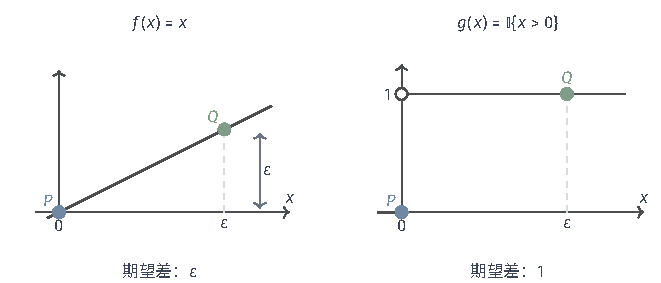
\includegraphics[width=\linewidth]{figures/02-mathematical-preliminaries-lower/01-random-variables-distributions-and-causality/tikz/information-small-shift-task/figure.pdf}
  \caption{同一小位移对两种固定评价的影响。取\(P=\delta_0\)、
  \(Q=\delta_\varepsilon\)、\(\varepsilon>0\)，底层距离为绝对值。
  左图的\(1\)-Lipschitz函数\(f(x)=x\)变化\(\varepsilon\)；
  右图的事件函数\(\mathbb I\{x>0\}\)变化\(1\)。横向位置仅作示意，
  结论对任意正的\(\varepsilon\)成立。}
  \label{fig:information-small-shift-task}
\end{figure}

MMD提供另一种敏感性约束。若同一损失\(f\)属于核\(k\)的RKHS
\(\mathcal H_k\)，且核均值存在，则再生性质和Cauchy--Schwarz不等式给出
\[
  |\mathbb E_Pf-\mathbb E_Qf|
  =|\langle f,\bm\mu_P-\bm\mu_Q\rangle_{\mathcal H_k}|
  \leq\|f\|_{\mathcal H_k}\operatorname{MMD}_k(P,Q).
\]
下标\(k\)显式标明这里沿用的核空间和MMD。
必须知道\(f\)属于该空间及其范数；核具有特征性只保证分离分布，
不自动给出任意任务函数的有限范数。
同样，若底层成本只比较图像亮度，而任务依赖没有计入成本的位置变化，
不能声称损失相对于该成本是Lipschitz。成本与核是任务假设的一部分。

\subsection{指数矩约束下的期望响应}
\label{sec:information-change-measure}

有些损失没有统一上界，也难以给出输入空间的敏感常数，
但在参考分布下可控制其尾部。第~\ref{sec:rv-change-measure}节
允许用密度比换测度；下面用KL和指数矩代替密度比的逐点控制。
证明的关键是指数倾斜：按\(e^f\)重新加权参考分布，使较大函数值获得更多质量。

\begin{theorem}[Donsker--Varadhan变分表达]
\label{thm:information-donsker-varadhan}
设\(P\ll Q\)。对每个有界可测实函数\(f\)，
\begin{equation}
  D_{\mathrm{KL}}(P\Vert Q)
  \geq\mathbb E_Pf-\log\mathbb E_Qe^f.
  \label{eq:information-dv-lower}
\end{equation}
而且在扩展实数意义下，
\begin{equation}
  D_{\mathrm{KL}}(P\Vert Q)
  =\sup_{f\ \text{有界可测}}\{\mathbb E_Pf-\log\mathbb E_Qe^f\}.
  \label{eq:information-dv-variational}
\end{equation}
\end{theorem}
\begin{proof}
给定有界\(f\)，令\(Z_f=\mathbb E_Qe^f\)，并定义
\[
  \frac{\mathrm dQ_f}{\mathrm dQ}=\frac{e^f}{Z_f}.
\]
因\(0<Z_f<\infty\)，且密度比严格正，\(Q_f\)与\(Q\)等价。
若\(D_{\mathrm{KL}}(P\Vert Q)<\infty\)，对数密度比可积，
乘法法则给出完整的倾斜恒等式
\[
\begin{aligned}
  D_{\mathrm{KL}}(P\Vert Q_f)
  &=\mathbb E_P\left[\log\frac{\mathrm dP}{\mathrm dQ}-f+\log Z_f\right]\\
  &=D_{\mathrm{KL}}(P\Vert Q)-\mathbb E_Pf+\log Z_f.
\end{aligned}
\]
左侧非负即得下界；若原KL无限，右侧有限，下界仍成立。

为证明上确界恰好等于KL，不能直接假设\(\log(\mathrm dP/\mathrm dQ)\)有界。
记\(L=\mathrm dP/\mathrm dQ\)，在\(L=0\)处令\(\log L=-\infty\)，取
\[
  f_n=\max\{-n,\min\{\log L,n\}\}.
\]
由于\(P(L=0)=0\)，且
\(\mathbb E_P(\log L)^-=\int_{\{L<1\}}-L\log L\,\mathrm dQ<\infty\)，
负部由支配收敛、正部由单调收敛可知
\(\mathbb E_Pf_n\to D_{\mathrm{KL}}(P\Vert Q)\)，允许极限无限。
另一方面，\(e^{f_n}\to L\)，且\(e^{f_n}\leq1+L\)。
在\(Q\)下支配收敛给出\(\mathbb E_Qe^{f_n}\to1\)，
故对应变分值趋向KL。结合已证上界，得到等式。
若\(\log L\)本身有界，它直接取到等号；一般只保证截断序列逼近。
\end{proof}

取两点均匀参考分布\(Q=(1/2,1/2)\)，\(f=(0,\log3)\)，则
\(Z_f=2\)、\(Q_f=(1/4,3/4)\)。此时
\(\mathbb E_{Q_f}f=(3/4)\log3\)，
\(D_{\mathrm{KL}}(Q_f\Vert Q)=(3/4)\log3-\log2\)，
两者之差正是\(\log Z_f\)。
这次倾斜只改变概率权重，没有改变样本的取值。

现在令\(g\)允许无界。假设\(P\ll Q\)、\(g\in L^1(P)\)，并且对所选
\(\lambda>0\)有\(\mathbb E_Qe^{\lambda g}<\infty\)。
取\(g_n=\max\{-n,\min\{g,n\}\}\)，将定理用于\(\lambda g_n\)。
因\(|g_n|\leq|g|\)、\(e^{\lambda g_n}\leq1+e^{\lambda g}\)，
分别在\(P,Q\)下支配收敛，得到
\begin{equation}
  \mathbb E_Pg
  \leq\frac{D_{\mathrm{KL}}(P\Vert Q)+\log\mathbb E_Qe^{\lambda g}}{\lambda}.
  \label{eq:information-change-measure-expectation}
\end{equation}
KL有限才能让这个界提供有限的控制。
若还知道\(g\in L^1(Q)\)，且在\(Q\)下对所有\(t\in\mathbb R\)满足
\[
  \log\mathbb E_Qe^{t(g-\mathbb E_Qg)}\leq t^2\sigma^2/2,
\]
则分别对\(g-\mathbb E_Qg\)和其相反数应用上式，得到
\[
  |\mathbb E_Pg-\mathbb E_Qg|
  \leq\frac{D_{\mathrm{KL}}(P\Vert Q)}{\lambda}+\frac{\lambda\sigma^2}{2}.
\]
当KL与\(\sigma^2\)都严格正且有限时，
取\(\lambda=\sqrt{2D_{\mathrm{KL}}(P\Vert Q)/\sigma^2}\)，得到
\begin{equation}
  |\mathbb E_Pg-\mathbb E_Qg|
  \leq\sqrt{2\sigma^2D_{\mathrm{KL}}(P\Vert Q)}.
  \label{eq:information-subgaussian-change-measure}
\end{equation}
KL为零时\(P=Q\)；\(\sigma^2=0\)时\(g\)在\(Q\)下为常量，
由绝对连续在\(P\)下也如此，所以这两个边界情形仍成立。
对\(Q=\mathcal N(0,1)\)、\(P=\mathcal N(m,1)\)、\(g(x)=x\)，
方差代理为\(1\)，KL为\(m^2/2\)，上界恰等于真实期望差\(|m|\)。
这个界固定了评价函数及两张概率规律。若评价函数又根据同一批记录选出，函数与样本会产生联合依赖；第~\ref{sec:information-data-dependent-evaluation}节将在上述期望响应工具上处理这种选择。

\section{概率分布的优化}
\label{sec:information-variational-learning}

比较分布时，两张规律已经给出；优化分布时，至少一张规律需要选择。收益和矩条件可以决定希望得到的规律；给定目标与候选表示后，可以求最接近目标的分布；固定两个边缘以后，还可以选择成本最小的联合配对。三项任务改变的未知量不同，下面各自建立可行集合和目标，再核对最优解的存在与求解条件。

\subsection{目标约束下的分布选择}
\label{sec:information-target-distribution}

为了得到一张新的概率规律，可以规定平均收益，并限制它偏离参考分布的程度；也可以只给出均值等矩条件，在相容规律中最大化熵。此时待求对象是目标分布本身。约束确定可行范围，收益或熵确定选择方向，指数形式则由这些优化条件推导出来。

\subsubsection{参考分布下的收益与偏离权衡}
\label{sec:information-gibbs-optimization}

设\(P_0\)是可以采样的参考规律，\(f\)为有界可测收益。
只追求最大收益可能把质量全部集中到极少数点；
同时扣除偏离参考规律的KL，就得到下面的分布优化。
\begin{theorem}[Gibbs变分式]
\label{thm:information-gibbs-variational}
对有界可测\(f\)，
\begin{equation}
  \log\mathbb E_{P_0}e^f
  =\sup_{Q\ll P_0}\{\mathbb E_Qf-D_{\mathrm{KL}}(Q\Vert P_0)\}.
  \label{eq:information-gibbs-variational}
\end{equation}
KL无限时目标约定为\(-\infty\)，唯一最优分布为
\[
  \frac{\mathrm dQ^\star}{\mathrm dP_0}
  =\frac{e^f}{Z_f},\qquad Z_f=\mathbb E_{P_0}e^f.
\]
\end{theorem}
\begin{proof}
有界性保证\(0<Z_f<\infty\)，且\(Q^\star\)与\(P_0\)等价。
对任何有限KL的\(Q\ll P_0\)，
\[
  \log\frac{\mathrm dQ}{\mathrm dQ^\star}
  =\log\frac{\mathrm dQ}{\mathrm dP_0}-f+\log Z_f.
\]
各项在\(Q\)下可积，故倾斜恒等式给出
\[
  \mathbb E_Qf-D_{\mathrm{KL}}(Q\Vert P_0)
  =\log Z_f-D_{\mathrm{KL}}(Q\Vert Q^\star)\leq\log Z_f.
\]
无限KL候选的目标已为\(-\infty\)。对\(Q^\star\)，
\(\log(\mathrm dQ^\star/\mathrm dP_0)=f-\log Z_f\)有界，
所以自身收益与KL都有限，可以直接代入取到等号。
Gibbs不等式的等号条件说明最优分布唯一。
\end{proof}

这里优化的是分布，Donsker--Varadhan表达优化的则是测试函数；
两条变分式共用同一倾斜恒等式，却交换了固定对象和优化对象。
允许无界\(f\)时，至少需要\(0<Z_f<\infty\)才能定义\(Q^\star\)；
若还满足\(\mathbb E_{P_0}[e^f|f|]<\infty\)，
则\(f\in L^1(Q^\star)\)，最优表达中的两项都有限。
对其他候选，也须限制到\(f\in L^1(Q)\)且KL有限的定义域。

只有归一化常数有限并不够。例如在整数\(k\geq1\)上取
\(P_0(k)=C e^{-k}/k^2\)、\(f(k)=k\)，其中\(C\)归一化\(P_0\)。
则\(Z_f=C\sum_{k\geq1}k^{-2}<\infty\)，而\(Q^\star(k)\)正比于\(k^{-2}\)，
导致\(\mathbb E_{Q^\star}f=\infty\)且KL无限。
此时不能把\(Q^\star\)代入\(\infty-\infty\)。
若\(f\)为有限实值且\(Z_f<\infty\)，令
\(Z_n=\mathbb E_{P_0}[e^f\mathbb I_{\{|f|\leq n\}}]\)，在\(Z_n>0\)时取
\[
  \frac{\mathrm dQ_n}{\mathrm dP_0}
  =\frac{e^f\mathbb I_{\{|f|\leq n\}}}{Z_n}.
\]
其收益和KL有限，目标恰为\(\log Z_n\to\log Z_f\)。
因而在有限目标定义域上仍可逼近上确界，不必有可直接代入的最优分布。

对有界收益\(r\)加入温度\(\beta>0\)，令\(f=r/\beta\)，可得
\[
  \sup_{Q\ll P_0}\{\mathbb E_Qr-\beta D_{\mathrm{KL}}(Q\Vert P_0)\}
  =\beta\log\mathbb E_{P_0}e^{r/\beta},\qquad
  Q^\star\propto P_0e^{r/\beta}.
\]
较小温度更偏向高收益区域，也可能使重要性权重集中、采样方差增大。
KL正则描述相对于\(P_0\)的概率偏离；若某种失败事件必须受控，
仍需用上一节的风险迁移条件或另加约束，不能把正则项本身当成安全保证。

\subsubsection{矩约束下的最大熵选择}
\label{sec:information-maximum-entropy}

若只知道均值或协方差，没有指定收益函数，哪些分布与这些信息相容？
\term{最大熵原理}在相容分布中选择熵最大的一个。
它把“不过度集中”落实到一个明确的优化准则，不表示该分布已被观测证明为真；
参考测度和矩约束仍是建模选择。

固定参考测度\(\mu\)，要求密度\(p\)满足
\[
  \int p\,\mathrm d\mu=1,\qquad
  \int \bm T(x)p(x)\,\mathrm d\mu(x)=\bm\tau.
\]
若存在有限参数\(\bm\lambda\)，使
\[
  p_{\bm\lambda}(x)
  =\exp\{\bm\lambda^\top\bm T(x)-A(\bm\lambda)\},\qquad
  A(\bm\lambda)=\log\int e^{\bm\lambda^\top\bm T(x)}\,\mathrm d\mu(x)<\infty
\]
归一化并满足这些矩约束，则它是最大熵的候选。
形式上，对熵加归一化和矩约束的Lagrange项，密度方向的一阶条件为
\(-\log p-1+\bm\lambda^\top\bm T+a=0\)，从而给出上述指数形式。
但这一步没有证明解存在，也没有处理所有无限维变分的合法性；
真正的最优性可由KL直接核验。

对任意同样可行、统计量可积且熵有限的密度\(p\)，若候选自身也满足这些有限性条件，
\[
\begin{aligned}
  D_{\mathrm{KL}}(p\Vert p_{\bm\lambda})
  &=\int p\log p\,\mathrm d\mu-\bm\lambda^\top\bm\tau+A(\bm\lambda)\\
  &=-h_\mu(p)+h_\mu(p_{\bm\lambda})\geq0.
\end{aligned}
\]
因此候选最大化熵，等号当且仅当两密度几乎处处相同。
矩约束不可达、配分函数无限或最大熵没有上界时，乘子方程不能弥补这些缺口。
即使最大熵分布存在，边界约束也可能只能由无穷自然参数的极限表示。

固定均值\(\bm m\)和正定协方差\(\bm\Sigma\)时，
\(q=\mathcal N(\bm m,\bm\Sigma)\)给出一个完整实例。
其对数密度为
\[
  \log q(\bm x)
  =-\frac d2\log(2\pi)-\frac12\log\det\bm\Sigma
   -\frac12(\bm x-\bm m)^\top\bm\Sigma^{-1}(\bm x-\bm m).
\]
任意具有同样均值和协方差的密度\(p\)都满足
\[
  \mathbb E_p[(\bm X-\bm m)^\top\bm\Sigma^{-1}(\bm X-\bm m)]
  =\operatorname{tr}(\bm\Sigma^{-1}\bm\Sigma)=d.
\]
因而\(\mathbb E_p\log q=\mathbb E_q\log q\)，在\(h(p)\)有限时，
\[
  D_{\mathrm{KL}}(p\Vert q)=h(q)-h(p)\geq0,\qquad
  h(p)\leq\frac12\log\{(2\pi e)^d\det\bm\Sigma\}.
\]
等号唯一对应高斯。这仍是在固定坐标和Lebesgue参考测度下比较微分熵。
协方差奇异时，分布被限制在低维仿射子空间，不能继续使用原空间中的密度公式；
须改用子空间参考测度。

指数形式还把分布优化与参数表示联系起来。
对前章的指数族
\[
  p_{\bm\eta}(x)
  =h(x)\exp\{\bm\eta^\top\bm T(x)-A(\bm\eta)\},
\]
在允许交换微分积分的自然参数内部，
\(\nabla A(\bm\eta)=\mathbb E_{\bm\eta}\bm T=\bm\tau\)，
\(\nabla^2A(\bm\eta)=\operatorname{Cov}_{\bm\eta}(\bm T)\)。
自然参数\(\bm\eta\)指定指数权重，均值参数\(\bm\tau\)指定统计量平均。
回用\BookChapterRef{chap:optimization}{卷1《数学准备：分析、几何与计算》第4章“最优化”}的凸共轭，定义
\begin{equation}
  A^\star(\bm\tau)
  =\sup_{\bm\eta}\{\bm\eta^\top\bm\tau-A(\bm\eta)\}.
  \label{eq:information-log-partition-conjugate}
\end{equation}
若\(\bm\tau=\nabla A(\bm\eta)\)由有限自然参数实现，凸性的一阶不等式给出
\(A(\bm\zeta)\geq A(\bm\eta)+\bm\tau^\top(\bm\zeta-\bm\eta)\)。
移项可知共轭上确界在\(\bm\eta\)达到，且
\[
  A^\star(\bm\tau)=\bm\eta^\top\bm\tau-A(\bm\eta)
  =\int p_{\bm\eta}\log\frac{p_{\bm\eta}}h\,\mathrm d\mu.
\]
最后一个量是相对于基准项\(h\)的负熵；若\(h\)本身为概率密度，它就是KL。
只有\(h=1\)时才能直接写成普通负熵。

两组参数能否在局部互换，还取决于统计量有无冗余。所谓最小表示，是指不存在非零向量
\(\bm a\)，使\(\bm a^\top\bm T(x)\)在基准测度\(h\,\mathrm d\mu\)下几乎处处为常量。
在自然参数空间的开内部，这个条件给出
\[
 \bm a^\top\operatorname{Cov}_{\bm\eta}(\bm T)\bm a
 =\operatorname{Var}_{\bm\eta}(\bm a^\top\bm T)>0
 \qquad(\bm a\neq\bm0),
\]
因为有限自然参数的指数因子严格为正，模型分布与基准测度具有相同的零测集。
所以协方差正定，\(\mathrm d\bm\tau=\nabla^2A\,\mathrm d\bm\eta\)的Jacobian可逆，
由逆函数定理可得两组参数局部一一对应。
若统计量有含常量项的仿射冗余，例如某一坐标恒为\(1\)，协方差就会奇异；
只排除不同统计量之间的线性组合还不够。

有限配置可以不预设每个均值都由有限参数实现，而直接覆盖闭可行域。
\begin{theorem}[有限配置上的配分函数与最大熵对偶]
\label{thm:information-finite-entropy-duality}
设\(D\)为有限非空配置集，\(\bm T:D\to\mathbb R^m\)，基准权重恒为\(1\)。
定义
\[
  A(\bm\theta)=\log\sum_{z\in D}e^{\langle\bm\theta,\bm T(z)\rangle},
  \qquad\mathcal M=\operatorname{conv}\{\bm T(z):z\in D\}.
\]
对\(\bm\mu\in\mathcal M\)，令
\[
  H^\star(\bm\mu)=\max_{q:\,\mathbb E_q\bm T=\bm\mu}H(q),
\]
其中\(q\)遍历\(D\)上的全部概率质量函数。则在整个\(\mathcal M\)上有
\(A^\star(\bm\mu)=-H^\star(\bm\mu)\)，在外部有\(A^\star=+\infty\)，且
\begin{equation}
  A(\bm\theta)=\max_{\bm\mu\in\mathcal M}
  \{\langle\bm\theta,\bm\mu\rangle+H^\star(\bm\mu)\}.
  \label{eq:information-finite-gibbs-duality}
\end{equation}
\end{theorem}
\begin{proof}
有限概率单纯形紧；给定可行均值后的约束闭且非空，熵在单纯形上连续，
因此每个\(H^\star(\bm\mu)\)都能达到。
令\(p_{\bm\theta}(z)=e^{\langle\bm\theta,\bm T(z)\rangle-A(\bm\theta)}\)。
对任意质量函数\(q\)，展开有限KL得到
\[
  \langle\bm\theta,\mathbb E_q\bm T\rangle+H(q)
  =A(\bm\theta)-D_{\mathrm{KL}}(q\Vert p_{\bm\theta})
  \leq A(\bm\theta),
\]
且在\(q=p_{\bm\theta}\)处取等号。把所有\(q\)按均值分组，
组内线性项相同，只需保留最大熵者，即得式~\eqref{eq:information-finite-gibbs-duality}。

为证明边界处也有共轭等式，在\(\mathcal M\)上令\(f=-H^\star\)，
在外部令\(f=+\infty\)。
取两个均值及其最大熵分布\(q_1,q_2\)，混合
\(tq_1+(1-t)q_2\)的均值为对应均值的凸组合。
熵凹性给出
\[
  H^\star(t\bm\mu_1+(1-t)\bm\mu_2)
  \geq H(tq_1+(1-t)q_2)
  \geq tH^\star(\bm\mu_1)+(1-t)H^\star(\bm\mu_2).
\]
所以\(f\)凸。
若\(\bm\mu_n\to\bm\mu\)且各均值可行，先取使最大熵值趋于上极限的子列，
再从对应的最大熵分布中取收敛子列\(q_{n_k}\to q\)。
有限维均值映射连续，故\(\mathbb E_q\bm T=\bm\mu\)；熵连续性给出
\[
  \limsup_nH^\star(\bm\mu_n)=H(q)\leq H^\star(\bm\mu).
\]
于是\(H^\star\)上半连续。又因\(\mathcal M\)闭，
扩展后的\(f\)在整个\(\mathbb R^m\)上下半连续。
由\(0\leq H^\star\leq\log|D|\)和\(\mathcal M\neq\varnothing\)，
\(f\)适当。前半证明已说明\(f^\star=A\)，
\BookTheoremRef{thm:opt-fenchel-moreau}{卷1《数学准备：分析、几何与计算》第4章“最优化”第4.4.3.2节“对偶下界与全局最优”}于是给出
\(A^\star=f^{\star\star}=f\)，包括边界均值和可行域外部。
此证明不要求共轭上确界由有限自然参数达到。
\end{proof}

\(\mathcal M\)是可实现统计量均值的凸包。
统计量由各局部配置的指示函数组成时，它称为边缘多面体；
属于该集合表示局部概率表能同时来自同一全局分布，
强于每张表单独归一化。例如两个二元变量的两张边缘表均令取值\(1\)的概率为\(0.1\)，
则联合表不可能同时要求\(P(X=1,Y=1)=0.9\)。
局部数字各自在\([0,1]\)内，并不足以保证共同可实现。

在\(\{0,1,2\}\)上要求\(\mathbb EX=1/2\)时，最大熵分布为
\(p_j=t^j/(1+t+t^2)\)。均值方程给出
\[
  \frac{t+2t^2}{1+t+t^2}=\frac12,\qquad
  3t^2+t-1=0,\qquad
  t=\frac{\sqrt{13}-1}{6}\approx0.4343.
\]
故\((p_0,p_1,p_2)\approx(0.6162,0.2676,0.1162)\)。
自然参数是\(\lambda=\log t\)，
\(H(p)=\log(1+t+t^2)-\lambda/2\)，与共轭负熵一致。
若均值改为边界值\(0\)，唯一可行分布为\(\delta_0\)，熵为零；
它由\(t\downarrow0\)、\(\lambda\to-\infty\)逼近，却没有有限自然参数表示。
这正是分布最优解存在与有限参数实现之间的区别。

\subsection{表示约束下的分布逼近}
\label{sec:information-elbo-approximation}

联合模型和观测可以确定一张后验分布，但归一化积分难以计算时，精确表示和采样仍可能不可行。我们把未知量改成可计算候选族中的密度\(q\)，以它逼近已经确定的后验。固定观测\(x\)和模型参数\(\bm\theta\)，设
\[
  0<p_{\bm\theta}(x)=\int p_{\bm\theta}(x,z)\,\mathrm dz<\infty,
  \qquad
  \pi(z)=p_{\bm\theta}(z\mid x).
\]
记候选密度为\(q\)。证据积分可能难算，候选\(q\)则允许采样和评价密度。

\begin{definition}[证据下界]
\label{def:information-elbo}
若\(q\ll\pi\)且\(D_{\mathrm{KL}}(q\Vert\pi)<\infty\)，定义
\term{证据下界}（evidence lower bound, ELBO）为
\[
  \mathcal L(q,\bm\theta;x)
  =\mathbb E_q\log\frac{p_{\bm\theta}(x,Z)}{q(Z)}.
\]
按对数比整体取期望，不要求\(\mathbb E_q\log p_{\bm\theta}(x,Z)\)
与\(\mathbb E_q\log q(Z)\)各自有限。
\end{definition}

有限KL保证上述整体对数比可积，因为它等于
\(\log p_{\bm\theta}(x)-\log(q/\pi)\)。
直接分解就得到
\begin{equation}
  \log p_{\bm\theta}(x)
  =\mathcal L(q,\bm\theta;x)+D_{\mathrm{KL}}(q\Vert p_{\bm\theta}(\cdot\mid x)).
  \label{eq:information-elbo-decomposition}
\end{equation}
因此它确为下界，等号当且仅当\(q=\pi\)。
若KL无限，可以把ELBO扩展为\(-\infty\)，
但应使用\(\mathcal L=\log p_{\bm\theta}(x)-D_{\mathrm{KL}}\)这一方向，
不把右侧的\(-\infty+\infty\)当作合法分解。

另一条常见推导先乘除\(q\)，再使用Jensen不等式。
这里重要性等号需要相反方向的覆盖条件\(\pi\ll q\)，
保证联合密度的正质量区域不会被\(q\)漏掉。
若同时满足\(q\ll\pi\)和上述可积性，则
\begin{align}
  \log p_{\bm\theta}(x)
  &=\log\mathbb E_q\left[\frac{p_{\bm\theta}(x,Z)}{q(Z)}\right]\notag\\
  &\geq\mathbb E_q\log\frac{p_{\bm\theta}(x,Z)}{q(Z)}
   =\mathcal L(q,\bm\theta;x).
  \label{eq:information-elbo-jensen}
\end{align}
只满足\(q\ll\pi\)时，KL分解仍成立，
但重要性期望实际为\(p_{\bm\theta}(x)\pi(\{q>0\})\)，可能小于证据。
例如\(\pi=(1/2,1/2)\)、\(q=(1,0)\)，KL为\(\log2\)，
ELBO是\(\log p_{\bm\theta}(x)-\log2\)，而重要性期望只恢复一半证据。
反过来，若\(\pi=(1,0)\)、\(q=(1/2,1/2)\)，虽完整覆盖目标，
但\(q\)在零后验区域放了质量，反向KL无限。两种支持要求不能互相代替。

表~\ref{tab:information-candidate-support}将支持方向与两种计算并列。完整恢复证据要求候选覆盖后验，
而有限的\(D_{\mathrm{KL}}(q\Vert\pi)\)还要求候选不在零后验区域放置质量；两者控制的对象不同。
\begin{table*}[htbp]
  \centering\small
  \begin{tabularx}{\linewidth}{XXcccc}
    \toprule
    后验\(\pi\) & 候选\(q\) & \(q\ll\pi\) & \(\pi\ll q\) & \(D_{\mathrm{KL}}(q\Vert\pi)\) & 证据恢复比例\\
    \midrule
    \((1/2,1/2)\) & \((1,0)\) & 是 & 否 & \(\log2\) & \(1/2\)\\
    \((1,0)\) & \((1/2,1/2)\) & 否 & 是 & \(+\infty\) & \(1\)\\
    \((1/2,1/2)\) & \((1/2,1/2)\) & 是 & 是 & \(0\) & \(1\)\\
    \bottomrule
  \end{tabularx}
  \caption{候选支持对KL与证据恢复的影响。两点分布共用同一取值集合，证据满足
  \(0<p_{\bm\theta}(x)<\infty\)。恢复比例为\(\mathbb E_q[p_{\bm\theta}(x,Z)/q(Z)]/p_{\bm\theta}(x)=\pi(\{q>0\})\)，
  比值仅在\(q>0\)处评价。表中的有限KL是具体例子的结果；一般空间中\(q\ll\pi\)不能单独保证KL有限。}
  \label{tab:information-candidate-support}
\end{table*}

固定模型后最大化ELBO，等价于在候选族\(\mathcal Q\)中最小化
\(D_{\mathrm{KL}}(q\Vert\pi)\)。
假设\(\mathcal Q\)中至少有一个有限KL的候选，并且实际候选\(q\)也具有有限KL。
此时族内下确界是有限的非负数，实际候选的KL可写为
\[
  D_{\mathrm{KL}}(q\Vert\pi)
  =\inf_{\widetilde q\in\mathcal Q}D_{\mathrm{KL}}(\widetilde q\Vert\pi)
   +\left[D_{\mathrm{KL}}(q\Vert\pi)
    -\inf_{\widetilde q\in\mathcal Q}D_{\mathrm{KL}}(\widetilde q\Vert\pi)\right].
\]
第一项是表示限制，第二项是未达到族内最优的求解误差。
在上述有限性条件下，即使最优候选不存在，这个按下确界的分解仍有效。
若候选族中的KL全部无限，就没有有限ELBO候选，不能用无穷减无穷定义求解误差。
若同时拟合\(\bm\theta\)，证据和后验也随之改变，
模型与真实数据规律的拟合误差是另一层问题，不等于这两项之和。

取\(Z\sim\mathcal N(0,1)\)、\(X\mid Z\sim\mathcal N(Z,1)\)，观测\(x=1\)。
配平方得到后验\(\mathcal N(1/2,1/2)\)，证据为\(\mathcal N(0,2)\)。
若\(q=\mathcal N(0,1)\)，
\[
\begin{aligned}
  \log p(x)&=-\tfrac12\log(4\pi)-\tfrac14\approx-1.5155,\\
  D_{\mathrm{KL}}(q\Vert\pi)
  &=\tfrac12\{2+\tfrac12-1+\log(1/2)\}\approx0.4034,\\
  \mathcal L(q;x)&\approx-1.9189.
\end{aligned}
\]
三者满足精确分解。多变量情形把\(q\)限制为分块独立族，
可能留下无法表示的后验相关性；求解更充分也不能消除这一表示限制。

分布蒸馏采用另一个给定目标：教师的条件分布\(P_{\mathrm T}(\cdot\mid x)\)。
在有限类别空间和固定输入权重下，最小化条件KL的平均
\(\mathbb E_XD_{\mathrm{KL}}(P_{\mathrm T}(\cdot\mid X)\Vert Q_{\bm\phi}(\cdot\mid X))\)
等价于教师软标签下的交叉熵，要求学生覆盖教师的正质量类别。
反向KL改由学生平均，支持要求和最优近似都会改变。
学生逼近教师，不自动意味着更接近真实标签规律。

联合配对还可以产生另一张待逼近的分布：给定一组候选以后，正样本位于哪个位置的条件概率。评分函数通过有限候选上的归一化来表示这张条件分布；表示能否恢复它，取决于评分函数类和候选的抽样规律。下面把一个联合配对样本与若干边缘负样本组成分类任务。
以一个具体的InfoNCE损失为例，取总候选数\(K\geq2\)，按目标联合分布抽取
\((X,Y_1)\)，再独立地按边缘\(P_Y\)抽取\(Y_2,\ldots,Y_K\)；
这些负样本彼此独立，也独立于\((X,Y_1)\)。对可测实值评分函数\(s\)，定义
\begin{equation}
 \mathcal L_K
 =\mathbb E\left[-\log
   \frac{\exp s(X,Y_1)}{\sum_{j=1}^K\exp s(X,Y_j)}\right].
 \label{eq:information-contrastive-loss}
\end{equation}
它把相对评分归一化为候选类别概率，再惩罚未能认出正样本的预测。
\(K\)包括一个正样本和\(K-1\)个负样本；期望针对上述全部抽样。
若该损失可积，则
\[
 \log K-\mathcal L_K\leq I(X;Y).
\]

这个下界可从分类熵推得。等价地，先在\(K\)个位置中均匀选正样本位置\(J\)，
令该位置与\(X\)按目标联合分布配对，其余位置仍为独立边缘样本。
记整组观测为\(W=(X,Y_1,\ldots,Y_K)\)。
同一个评分规则在各位置对称使用，所以平均分类损失仍为\(\mathcal L_K\)。记评分给出的类别概率为
\[
 q_s(j\mid W)=\frac{\exp s(X,Y_j)}{\sum_{u=1}^K\exp s(X,Y_u)}.
\]
有限实值评分使各类别概率严格为正。按真实位置后验计算交叉熵，并使用式~\eqref{eq:information-cross-entropy-decomposition}，得到
\[
 \mathcal L_K=H(J\mid W)+\mathbb E_W D_{\mathrm{KL}}\bigl(P_{J\mid W}\Vert q_s(\cdot\mid W)\bigr).
\]
这里\(H(J\mid W)\leq\log K\)，且假设分类损失可积，因此两项都有限。第二项明确度量评分表示对位置后验的逼近误差；其非负性也给出后面所需的熵下界。因此
\[
 \log K-\mathcal L_K\leq H(J)-H(J\mid W)=I(J;W).
\]
还需说明识别正样本位置的信息不会超过目标互信息。令\(P_j\)为给定\(J=j\)的
\(W\)分布，\(M=K^{-1}\sum_jP_j\)，并以完全独立规律
\(Q=P_X\otimes P_Y^{\otimes K}\)作参照。若\(I(X;Y)<\infty\)，
每个\(P_j\)相对于\(Q\)只有正样本配对这一项密度比，所以
\[
\begin{aligned}
 I(X;Y)&=\frac1K\sum_{j=1}^KD_{\mathrm{KL}}(P_j\Vert Q)\\
 &=\frac1K\sum_{j=1}^KD_{\mathrm{KL}}(P_j\Vert M)
      +D_{\mathrm{KL}}(M\Vert Q)\\
 &=I(J;W)+D_{\mathrm{KL}}(M\Vert Q)\geq I(J;W).
\end{aligned}
\]
中间等式将对数密度比拆成经过\(M\)的两项，再对\(j\)平均；
互信息无限时原下界自动成立。
又因分类损失非负，\(\log K-\mathcal L_K\leq\log K\)，
有限候选数确实会限制这个下界的最大数值。
不符合采样假设时，不能把优化该分类目标直接解释为增加原分布的互信息；
即使下界合法，也不自动保证校准、语义质量或下游风险。

\subsection{边缘约束下的分布耦合}
\label{sec:information-coupling-optimization}

把两个固定边缘\(P,Q\)配成联合分布时，可以有许多不同的配对。未知量是
\(\gamma\in\Pi(P,Q)\)，每个候选都须保留这两个边缘。给出位置之间的搬运成本后，最优配对决定哪些质量配到哪些位置。独立乘积说明可行集合非空，但它未必使平均成本最小。
定义~\ref{def:information-coupling}与式~\eqref{eq:information-kantorovich-transport}
已经给出可行集合和成本，这里补足最小值的存在与有限求解。

\subsubsection{边缘约束下的最优耦合存在}
\label{sec:information-optimal-coupling-existence}

有限表格不会丢失总质量，但一般空间中的一列近最优方案可能把质量送往越来越远处。
证明存在性，要同时防止质量逃逸、保住固定边缘，并使极限成本不增加。
第~\ref{sec:rv-weak-convergence}节的概率测度弱收敛及紧性正好服务这三步。
这里不重新定义它们：变化对象是乘积空间上的概率测度，
测试函数是有界连续函数；这不同于泛函分析中固定线性空间内由连续线性泛函
检验的弱拓扑。二者都有“弱收敛”这一中文名称，但不能不说明对象就互换结论。

\begin{theorem}[最优耦合存在]
\label{thm:information-optimal-coupling-existence}
设\(\mathcal X,\mathcal Y\)为Polish空间，\(P,Q\)为其Borel概率测度。
若成本\(c:\mathcal X\times\mathcal Y\to[0,\infty]\)下半连续，
且至少有一个\(\gamma_0\in\Pi(P,Q)\)满足\(\int c\,\mathrm d\gamma_0<\infty\)，
则存在有限成本耦合\(\gamma^\star\)达到
\(\mathcal T_c(P,Q)=\inf_{\gamma\in\Pi(P,Q)}\int c\,\mathrm d\gamma\)。
\end{theorem}
\begin{proof}
可行集合非空，且成本非负、有有限可行值，所以最优下确界有限。
取近最优序列\(\gamma_n\in\Pi(P,Q)\)，使
\(\int c\,\mathrm d\gamma_n\to\mathcal T_c(P,Q)\)。

Polish空间上的Borel概率测度紧。
任给\(\varepsilon>0\)，分别选择紧集\(K_{\mathcal X},K_{\mathcal Y}\)，使
\(P(K_{\mathcal X}^{\mathsf c})<\varepsilon/2\)、
\(Q(K_{\mathcal Y}^{\mathsf c})<\varepsilon/2\)。
其乘积紧，且任意可行耦合都满足
\[
  \gamma((K_{\mathcal X}\times K_{\mathcal Y})^{\mathsf c})
  \leq P(K_{\mathcal X}^{\mathsf c})+Q(K_{\mathcal Y}^{\mathsf c})
  <\varepsilon.
\]
因边缘固定，这个紧集对全部\(\gamma\)同时适用，
从而\((\gamma_n)\)一致紧。
乘积空间仍为Polish空间，定理~\ref{thm:rv-prokhorov}给出子列
\(\gamma_{n_k}\Rightarrow\gamma^\star\)。

对任意有界连续\(a:\mathcal X\to\mathbb R\)，函数
\((x,y)\mapsto a(x)\)有界连续，故
\[
  \int a(x)\,\mathrm d\gamma^\star(x,y)
  =\lim_k\int a(x)\,\mathrm d\gamma_{n_k}(x,y)=\int a\,\mathrm dP.
\]
有界连续函数区分Borel概率测度，因此\(\gamma^\star\)的第一边缘为\(P\)。
同理第二边缘为\(Q\)，所以极限仍可行。

最后，对非负下半连续成本使用定理~\ref{thm:rv-portmanteau}：
\[
  \int c\,\mathrm d\gamma^\star
  \leq\liminf_k\int c\,\mathrm d\gamma_{n_k}
  =\mathcal T_c(P,Q).
\]
可行性又给出反向不等式，所以等号成立且成本有限。
\end{proof}

最后一步的积分测度随\(k\)改变，不能用固定测度下的Fatou引理直接替代。
非负性避免成本的负部失控，下半连续性保证极限不会突然增加成本；
若修改这些假设，需要另给能实现同样作用的条件。
存在联合耦合也不保证存在确定搬运映射。
例如\(P=\delta_0\)、\(Q=(\delta_{-1}+\delta_1)/2\)时，
唯一来源点必须把质量分成两半，任何单值映射都只能把它送到一个点。

\subsubsection{有限空间下的最优耦合求解}
\label{sec:information-finite-transport}

设来源点为\(x_i\)、目标点为\(y_j\)，概率向量为\(\bm p,\bm q\)，
各成本\(c_{i,j}\)有限且非负。搬运表\(\bm\gamma\)的行和是来源质量，
列和是目标质量，问题为
\[
  \min_{\gamma_{i,j}\geq0}\sum_{i,j}c_{i,j}\gamma_{i,j},
  \qquad \sum_j\gamma_{i,j}=p_i,\quad\sum_i\gamma_{i,j}=q_j.
\]
独立表\(\gamma_{i,j}=p_iq_j\)可行。
约束集合闭，且每个元素在\([0,1]\)内，因此它是紧多面体，
线性目标可以取到最小值。

回用\BookChapterRef{chap:optimization}{卷1《数学准备：分析、几何与计算》第4章“最优化”}线性规划，为两组边缘约束引入势函数
\(u_i,v_j\)，保留\(\gamma_{i,j}\geq0\)作为取下确界的定义域：
\begin{align}
  \mathcal L(\bm\gamma,\bm u,\bm v)
  &=\sum_{i,j}c_{i,j}\gamma_{i,j}
    +\sum_i u_i\left(p_i-\sum_j\gamma_{i,j}\right)
    +\sum_j v_j\left(q_j-\sum_i\gamma_{i,j}\right)\notag\\
  &=\sum_i u_ip_i+\sum_jv_jq_j
    +\sum_{i,j}(c_{i,j}-u_i-v_j)\gamma_{i,j}.
  \label{eq:information-discrete-ot-lagrangian}
\end{align}
如果某个系数\(c_{i,j}-u_i-v_j<0\)，将对应非负变量趋向无穷，
Lagrangian下确界就是\(-\infty\)。
若全部系数非负，下确界可在\(\bm\gamma=\bm0\)取到，
值为\(\sum_i u_ip_i+\sum_jv_jq_j\)。
这里消元时边缘等式已进入Lagrangian，不再限制\(\bm\gamma\)，
所以零表虽不是原问题的可行表，却可以用于计算对偶函数。
于是
\[
  g(\bm u,\bm v)=
  \begin{cases}
    \sum_i u_ip_i+\sum_jv_jq_j,&u_i+v_j\leq c_{i,j}\text{ 对所有 }i,j,\\
    -\infty,&\text{否则}.
  \end{cases}
\]
最大化它得到
\begin{equation}
  \max_{\bm u,\bm v}
  \left\{\sum_i u_ip_i+\sum_jv_jq_j:\ u_i+v_j\leq c_{i,j}\right\}.
  \label{eq:information-discrete-ot-dual}
\end{equation}
势函数约束来自消元后下确界有限的必要充分条件，不是额外猜出的搬运规则。
对任意原始可行表，将\(u_i+v_j\leq c_{i,j}\)逐项乘\(\gamma_{i,j}\)
并求和，立刻得到对偶值不超过搬运成本。
有限维原问题可行且最优值有限，线性规划强对偶又保证两者最优值相等。

取来源和目标位置均为\(0,2\)，令\(\bm p=(3/4,1/4)\)、\(\bm q=(1/4,3/4)\)，
\(c_{i,j}=|x_i-y_j|\)。全部可行表都能写成
\[
  \bm\gamma(a)=
  \begin{pmatrix}
    a&3/4-a\\
    1/4-a&a
  \end{pmatrix},\qquad 0\leq a\leq1/4.
\]
对角线成本为零，两个非对角线成本均为\(2\)，
故总成本为\(2-4a\)，在\(a=1/4\)处最小：
\[
  \bm\gamma^\star=
  \begin{pmatrix}1/4&1/2\\0&1/4\end{pmatrix},\qquad
  \sum_{i,j}c_{i,j}\gamma^\star_{i,j}=1.
\]
对偶取\(\bm u=(0,-2)\)、\(\bm v=(0,2)\)，四项和依次为
\(0,2,-2,0\)，均不超过对应成本\(0,2,2,0\)。
对偶值为
\[
  \bm u^\top\bm p+\bm v^\top\bm q
  =-2(1/4)+2(3/4)=1.
\]
弱对偶已足以核验最优性：所有可行表成本至少为\(1\)，而上表恰好达到。
图~\ref{fig:information-transport-tables}比较这个表与独立配对，
说明相同行列边缘不能决定搬运成本。
\begin{figure}[htbp]
  \centering
  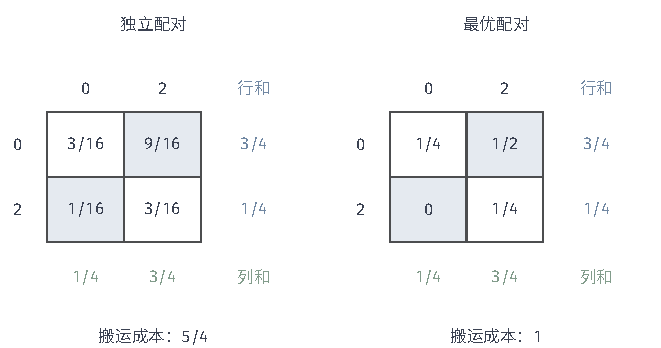
\includegraphics[width=\linewidth]{figures/02-mathematical-preliminaries-lower/01-random-variables-distributions-and-causality/tikz/information-transport-tables/figure.pdf}
  \caption{同一边缘约束下的两张搬运表。来源和目标都位于\(0,2\)，
  蓝色行和为\(\bm p=(3/4,1/4)\)，绿色列和为\(\bm q=(1/4,3/4)\)。
  浅色单元格承担非零距离成本。独立表的成本为\(5/4\)，最优表为\(1\)；
  正文的势函数给出与最优表相等的对偶值。}
  \label{fig:information-transport-tables}
\end{figure}

\section{参数化分布的迭代优化}
\label{sec:information-global-local-geometry}
\label{sec:information-fisher-geometry}

分布选择、逼近和耦合都可以通过候选参数来求解；参数表示须保留各自的可行约束。设当前候选族为\(\{P_{\bm\theta}:\bm\theta\in\Theta\}\)。当算法更新参数时，我们还要比较每一步造成的分布变化：相同的欧氏参数步长，是否具有相同的概率意义？高斯均值的同样位移在小噪声下更容易辨认，
参数坐标的单位也可以任意缩放，因此需要根据分布自身定义局部步长。
本节回用优化与流形中的切向量、度量工具，但度量由概率模型的局部KL建立。
若参数化没有自动满足矩或边缘约束，仍要显式处理可行域，不能直接作无约束更新。

\subsection{参数变化下的分布距离}
\label{sec:information-local-metric}

改变参数值通常会改变分布；更换表示同一分布的坐标则不应该改变几何对象。
先分析前一种真实扰动，再检查后一种坐标变化。
得分和Fisher信息矩阵的正式定义沿用前章定义~\ref{def:information-fisher-matrix}，
这里增加把它们连接到局部KL所需的正则条件。

\paragraph{小参数变化下的分布差异}
\label{sec:information-local-kl}

设参数域\(\Theta\subseteq\mathbb R^d\)，共同参考测度为\(\mu\)。
固定内点\(\bm\theta\)，假设存在开邻域\(U\)和共同可测支持\(S\)，
使所有\(\bm\eta\in U\)都在\(S\)上满足\(p_{\bm\eta}>0\)，在外部为零。
再假设\(p_{\bm\eta}(x)\)对参数二阶连续可微，
其一、二阶导数分别由\(\mu\)-可积函数在\(U\)上一致控制。
这些条件允许对归一化等式交换一、二阶微分和积分。
沿用得分记号\(\bm s_{\bm\theta}(x)=\nabla_{\bm\theta}\log p_{\bm\theta}(x)\)，有
\begin{equation}
  \mathbb E_{\bm\theta}\bm s_{\bm\theta}(X)
  =\int\nabla_{\bm\theta}p_{\bm\theta}(x)\,\mathrm d\mu(x)=\bm0.
  \label{eq:information-score-zero}
\end{equation}

进一步要求
\[
  \mathbb E_{\bm\theta}\|\bm s_{\bm\theta}(X)\|_2^2<\infty,\qquad
  \mathbb E_{\bm\theta}
  \|\nabla^2_{\bm\theta}\log p_{\bm\theta}(X)\|_{\mathrm{op}}<\infty.
\]
此时Fisher矩阵
\(\bm F(\bm\theta)=\mathbb E_{\bm\theta}[\bm s_{\bm\theta}\bm s_{\bm\theta}^\top]\)
有限。乘积法则给出
\[
  \nabla^2_{\bm\theta}p_{\bm\theta}
  =p_{\bm\theta}
   \{\nabla^2_{\bm\theta}\log p_{\bm\theta}
      +\bm s_{\bm\theta}\bm s_{\bm\theta}^\top\}.
\]
两边积分，左侧由二阶微分归一化等式为零，故
\begin{equation}
  \bm F(\bm\theta)
  =-\mathbb E_{\bm\theta}\nabla^2_{\bm\theta}\log p_{\bm\theta}(X).
  \label{eq:information-fisher-hessian-identity}
\end{equation}
这就是此处使用的信息恒等式。
不能只对得分的零均值求导而忽略积分权重\(p_{\bm\theta}\)也依赖参数。
共同支持同样重要：例如均匀族\(\operatorname{Unif}(0,\theta)\)
有移动边界，内部对数密度导数为\(-1/\theta\)，其均值不为零；
这不反驳恒等式，而是没有满足推导条件。

\begin{theorem}[KL的局部二阶展开]
\label{thm:information-kl-local-fisher}
在上述共同支持、交换微分及可积条件下，进一步设\(U\)可取为凸集，
且对\(P_{\bm\theta}\)-几乎处处的\(x\)，
\(\nabla^2_{\bm\eta}\log p_{\bm\eta}(x)\)在\(\bm\theta\)处连续。
假设存在\(M\in L^1(P_{\bm\theta})\)，使
\[
  \sup_{\bm\eta\in U}
  \|\nabla^2_{\bm\eta}\log p_{\bm\eta}(x)\|_{\mathrm{op}}\leq M(x)
\]
几乎处处成立。则当\(\bm\delta\to\bm0\)且\(\bm\theta+\bm\delta\in U\)时，
\begin{equation}
  D_{\mathrm{KL}}(P_{\bm\theta}\Vert P_{\bm\theta+\bm\delta})
  =\tfrac12\bm\delta^\top\bm F(\bm\theta)\bm\delta
   +o(\|\bm\delta\|_2^2).
  \label{eq:information-kl-fisher-expansion}
\end{equation}
\end{theorem}
\begin{proof}
对几乎处处的固定\(x\)，沿线段\(\bm\theta+t\bm\delta\)作带积分余项的Taylor展开：
\[
\begin{aligned}
  \log p_{\bm\theta+\bm\delta}(x)-\log p_{\bm\theta}(x)
  &=\bm\delta^\top\bm s_{\bm\theta}(x)\\
  &\quad+\int_0^1(1-t)\bm\delta^\top
  \left.\nabla^2_{\bm\eta}\log p_{\bm\eta}(x)
  \right|_{\bm\eta=\bm\theta+t\bm\delta}
  \bm\delta\,\mathrm dt.
\end{aligned}
\]
得分二阶可积保证一阶可积，余项绝对值被
\(\|\bm\delta\|_2^2M(x)/2\)控制，
所以整个对数密度比在\(P_{\bm\theta}\)下可积。
按该分布取负期望，一阶项由式~\eqref{eq:information-score-zero}消失。
在乘积测度\(P_{\bm\theta}\otimes\mathrm dt\)下，
Hessian的连续性和可积控制允许支配收敛，故
\[
  \int_0^1(1-t)\mathbb E_{\bm\theta}
  \left[
    \left.\nabla^2_{\bm\eta}\log p_{\bm\eta}(X)
    \right|_{\bm\eta=\bm\theta+t\bm\delta}
  \right]\mathrm dt
  =\tfrac12\mathbb E_{\bm\theta}\nabla^2_{\bm\theta}
    \log p_{\bm\theta}(X)+o(1)
\]
在有限维矩阵算子范数下成立。
代入信息恒等式，左右乘\(\bm\delta^\top,\bm\delta\)，
矩阵的\(o(1)\)便成为\(o(\|\bm\delta\|_2^2)\)，得到结论。
\end{proof}

Fisher总半正定，但成为度量还需要得分满秩：
对每个\(\bm v\neq\bm0\)，都有
\(\mathbb E_{\bm\theta}(\bm v^\top\bm s_{\bm\theta})^2>0\)。
这恰好等价于\(\bm F(\bm\theta)\)正定；
从切向量看，没有非零参数方向在一阶上完全不改变分布。
局部可识别只排除附近参数产生同一分布，不能代替这个微分条件。
例如\(P_\theta=\mathcal N(\theta^3,\sigma^2)\)的参数表示一一对应，但
\[
  F(\theta)=9\theta^4/\sigma^2,\qquad
  D_{\mathrm{KL}}(P_0\Vert P_\delta)=\delta^6/(2\sigma^2).
\]
在零点Fisher为零，KL从六阶才开始变化；“不同参数可区分”不等于
“每个方向都有非零二阶曲率”。

\begin{definition}[Fisher度量]
\label{def:information-fisher-metric}
在Fisher矩阵正定的正则参数点，对切向量\(\bm u,\bm v\)定义
\term{Fisher度量}
\[
  g_{\bm\theta}(\bm u,\bm v)=\bm u^\top\bm F(\bm\theta)\bm v.
\]
\end{definition}
高斯位置族的\(F(\mu)=1/\sigma^2\)，局部长度为
\(|\mathrm d\mu|/\sigma\)，与均值移动的KL公式一致。
Bernoulli族\(P_p\)、\(0<p<1\)的得分在结果\(1,0\)上分别为
\(1/p,-1/(1-p)\)，故
\[
  F(p)=p/p^2+(1-p)/(1-p)^2=\frac1{p(1-p)}.
\]
固定\(p=0.2\)，精确KL为
\(0.2\log(0.2/q)+0.8\log(0.8/(1-q))\)，二阶式为\((q-0.2)^2/0.32\)。
在\(q=0.22\)处二者约为\(0.00119,0.00125\)；
当\(q\downarrow0\)时精确KL无限，固定二次式却仍有限。
图~\ref{fig:information-fisher-local}同时显示邻域近似和远离邻域后的差别，
不能把局部度量当成全域散度。
\begin{figure*}[htbp]
  \centering
  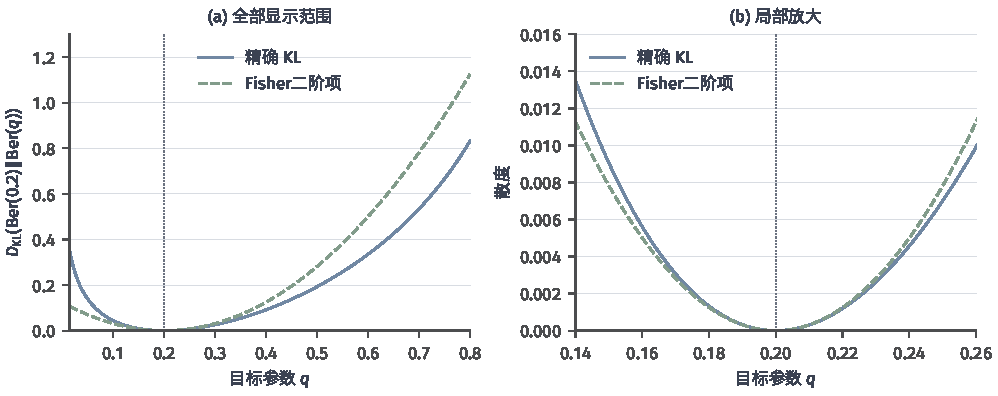
\includegraphics[width=\linewidth]{figures/02-mathematical-preliminaries-lower/01-random-variables-distributions-and-causality/matplotlib/information-fisher-local/figure.pdf}
  \caption{Bernoulli族在\(p=0.2\)处的Fisher局部近似（解析式教学图）。
  蓝实线为\(D_{\mathrm{KL}}(P_{0.2}\Vert P_q)\)，绿虚线为
  \((q-0.2)^2/[2(0.2)(0.8)]\)；右图放大邻域。图中\(0<q<1\)，
  二阶式只描述足够小的参数扰动。}
  \label{fig:information-fisher-local}
\end{figure*}

\paragraph{重参数化下的几何保持}
\label{sec:information-fisher-reparameterization}

令\(\bm\theta=\bm\theta(\bm\phi)\)为光滑局部可逆坐标变换，
Jacobian为\(\bm J=\partial\bm\theta/\partial\bm\phi\)。
在对应点\(P_{\bm\phi}=P_{\bm\theta(\bm\phi)}\)是同一张分布，
不是又施加一次统计扰动。链式法则给出
\[
  \bm s_{\bm\phi}=\bm J^\top\bm s_{\bm\theta},\qquad
  \bm F_{\bm\phi}=\bm J^\top\bm F_{\bm\theta}\bm J.
\]
因切向量满足\(\mathrm d\bm\theta=\bm J\,\mathrm d\bm\phi\)，
\[
  \mathrm d\bm\phi^\top\bm F_{\bm\phi}\mathrm d\bm\phi
  =\mathrm d\bm\theta^\top\bm F_{\bm\theta}\mathrm d\bm\theta.
\]
对同一标量目标\(L\)，梯度坐标变为
\(\bm g_{\bm\phi}=\bm J^\top\bm g_{\bm\theta}\)，
因此目标微分
\(\bm g_{\bm\phi}^\top\mathrm d\bm\phi
=\bm g_{\bm\theta}^\top\mathrm d\bm\theta\)也不变。
Fisher矩阵的数值会变，不变的是它作用于对应切向量所得到的二次型。

例如Bernoulli概率\(p\)改用logit坐标\(\phi=\log[p/(1-p)]\)，
\(\mathrm dp/\mathrm d\phi=p(1-p)\)，于是
\[
  F_\phi=\{p(1-p)\}^2F_p=p(1-p).
\]
一个坐标下的Fisher在边界附近变大，另一个变小，
但对同一分布扰动，
\((\mathrm dp)^2/[p(1-p)]=p(1-p)(\mathrm d\phi)^2\)。
坐标变换退化时不在上述局部可逆范围，例如立方高斯例子在零点的Jacobian为零。

在序贯模型中，先选对概率对象，比求逆更重要。
固定状态\(s\)，策略\(\pi_{\bm\theta}(a\mid s)\)的单步Fisher为
\[
  \bm F_s(\bm\theta)
  =\mathbb E_{A\sim\pi_{\bm\theta}(\cdot\mid s)}
    [\bm s_{\bm\theta}(s,A)\bm s_{\bm\theta}(s,A)^\top].
\]
若状态访问权重\(d(s)\)被指定并保持固定，
平均矩阵为\(\bm F_d=\mathbb E_{S\sim d}\bm F_S\)。
它衡量这一输入权重下的条件策略变化。
若把\(d_{\bm\theta}(s)\pi_{\bm\theta}(a\mid s)\)作为完整联合模型求导，
得分还包含\(\nabla\log d_{\bm\theta}(s)\)。
在正则条件下，条件策略得分均值为零，交叉项消失，联合Fisher成为
\[
  \bm F_{d_{\bm\theta}\pi_{\bm\theta}}
  =\bm F_{d_{\bm\theta}}^{\mathrm{state}}
    +\mathbb E_{d_{\bm\theta}}\bm F_S.
\]
它与把当前访问权重固定后得到的平均矩阵不是同一个对象。

第三个对象是完整轨迹Fisher。设初始分布和环境转移都不依赖参数，
参数只出现在固定有限时域\(T\)的条件动作核中。
假设共同支持和交换微分成立，各步得分二阶可积。
轨迹得分为\(\sum_{t=1}^T\bm s_t\)，其中
\(\mathbb E[\bm s_t\mid H_t]=\bm0\)，\(H_t\)为选择动作前的历史。
当\(u<t\)时，\(\bm s_u\)对\(H_t\)可测，因此
\[
  \mathbb E[\bm s_u\bm s_t^\top]
  =\mathbb E[\bm s_u\,\mathbb E(\bm s_t^\top\mid H_t)]=\bm0.
\]
展开外积便得到
\[
  \bm F_{\mathrm{trajectory}}
  =\sum_{t=1}^T\mathbb E[\bm F_{H_t}],
\]
而不是某个任意固定访问分布下的单步矩阵。
Markov策略下可把条件矩阵写成\(\bm F_{S_t}\)；
若访问权重取各时刻边缘的平均，轨迹矩阵等于对应平均矩阵的\(T\)倍。
环境或初始规律也含参数时，必须加入它们的得分，不能沿用策略独占参数的公式。

另一个常见混淆发生在样本矩阵与模型期望之间。
固定输入分布\(d\)，取条件高斯
\(Y\mid\bm X=\bm x\sim\mathcal N(\bm\theta^\top\bm x,\sigma^2)\)，
其中\(\sigma>0\)已知，\(\mathbb E_d\|\bm X\|^2<\infty\)。
同一观测的三个量为
\[
\begin{aligned}
  \bm s_{\bm\theta}(\bm x,y)
    &=\frac{y-\bm\theta^\top\bm x}{\sigma^2}\bm x,\\
  -\nabla^2_{\bm\theta}\log p_{\bm\theta}(y\mid\bm x)
    &=\frac{\bm x\bm x^\top}{\sigma^2},\\
  \bm s_{\bm\theta}\bm s_{\bm\theta}^\top
    &=\frac{(y-\bm\theta^\top\bm x)^2}{\sigma^4}\bm x\bm x^\top.
\end{aligned}
\]
按当前模型的条件分布平均时，残差平方期望为\(\sigma^2\)，
后两个矩阵的条件期望相同，再按\(d\)平均得到
\(\bm F=\mathbb E_d[\bm X\bm X^\top]/\sigma^2\)。
对一条样本，它们并不相等；残差为零时，得分外积甚至为零，
而非零输入的观测Hessian不为零。
如果真实响应规律不同于当前模型，残差平方的条件期望也可能不同，
经验得分外积的总体极限便不一定等于这个模型Fisher。
改变输入权重、使用观测Hessian或经验得分外积，都须重新说明正在近似哪个对象。

\subsection{基于分布几何的参数更新}
\label{sec:information-geometric-update}

有了局部长度和目标微分，就可以确定在给定分布变化预算内怎样下降。
这仍是原优化任务的局部求解步骤：若参数表示有约束，应在相应可行切空间中求解，
或结合约束优化和回缩；Fisher矩阵本身不会自动保持矩与固定边缘。

\paragraph{分布变化约束下的自然梯度}
\label{sec:information-natural-gradient-update}

设目标\(L(\bm\theta)\)可微，\(\bm g=\nabla L(\bm\theta)\)，
且\(\bm F(\bm\theta)\)正定。欧氏梯度是目标微分在欧氏内积下的代表；
改用Fisher内积，代表向量也应随之改变\scite{math-amari1998natural}
\begin{definition}[自然梯度]
\label{def:information-natural-gradient}
目标\(L\)的\term{自然梯度}（natural gradient）是满足
\[
  g_{\bm\theta}(\operatorname{grad}^{F}L,\bm v)
  =\nabla L(\bm\theta)^\top\bm v
  \quad\text{对所有切向量 }\bm v
\]
的唯一向量，即
\(\operatorname{grad}^{F}L=\bm F(\bm\theta)^{-1}\nabla L(\bm\theta)\)。
\end{definition}

把目标一阶线性化，把分布KL变化二阶近似，得到局部信赖域子问题
\begin{equation}
  \min_{\bm\delta}\bm g^\top\bm\delta
  \quad\text{s.t.}\quad
  \tfrac12\bm\delta^\top\bm F(\bm\theta)\bm\delta\leq\varepsilon.
  \label{eq:information-natural-gradient-trust-region}
\end{equation}
设\(\varepsilon>0,\bm g\neq\bm0\)。
Lagrangian为
\(\bm g^\top\bm\delta+\lambda(\bm\delta^\top\bm F\bm\delta/2-\varepsilon)\)，
驻点条件给出
\(\bm g+\lambda\bm F\bm\delta=\bm0\)。
非零线性目标的最小值在椭球边界，
代入\(\bm\delta=-\lambda^{-1}\bm F^{-1}\bm g\)得到
\(\lambda=\sqrt{\bm g^\top\bm F^{-1}\bm g/(2\varepsilon)}\)，所以
\begin{equation}
  \bm\delta^\star
  =-\sqrt{\frac{2\varepsilon}{\bm g^\top\bm F^{-1}\bm g}}\,
    \bm F^{-1}\bm g.
  \label{eq:information-natural-gradient-step}
\end{equation}

可以不依赖驻点必要条件，直接验证全局最优性。
令\(\bm u=\bm F^{1/2}\bm\delta\)，约束变为
\(\|\bm u\|_2\leq\sqrt{2\varepsilon}\)，目标变为
\((\bm F^{-1/2}\bm g)^\top\bm u\)。
Cauchy--Schwarz给出
\[
  (\bm F^{-1/2}\bm g)^\top\bm u
  \geq-\|\bm F^{-1/2}\bm g\|_2\sqrt{2\varepsilon}.
\]
等号在\(\bm u\)与\(-\bm F^{-1/2}\bm g\)同向并位于球面时达到，
代回正好得到上述解。若\(\bm g=\bm0\)，一阶目标处处为零，
子问题不再选出唯一方向，应考察高阶信息或停止条件。

\begin{example}[同一分布变化预算下的两个下降方向]
\label{ex:information-natural-gradient-ellipse}
设在当前参数点，局部Fisher矩阵与目标梯度为
\[
 \bm F=\begin{pmatrix}100&0\\0&1\end{pmatrix},
 \qquad \bm g=\begin{pmatrix}1\\1\end{pmatrix}.
\]
目标的一阶变化为\(\delta_1+\delta_2\)，但同样大小的第一维位移消耗的二次KL预算
是第二维的\(100\)倍。取局部预算\(\varepsilon=0.005\)，可行椭圆为
\(100\delta_1^2+\delta_2^2\leq0.01\)。普通欧氏下降方向是\(-\bm g\)，
自然下降方向是\(-\bm F^{-1}\bm g=-(0.01,1)^\top\)。
为公平比较，把两个方向都缩放到同一椭圆边界，得到
\[
 \bm\delta_{\mathrm E}=-\frac{0.1}{\sqrt{101}}(1,1)^\top,
 \qquad
 \bm\delta_{\mathrm F}=-\frac{0.1}{\sqrt{1.01}}(0.01,1)^\top.
\]
两者都恰好消耗\(0.005\)的二次预算，目标的一阶下降量分别为
\[
 -\bm g^\top\bm\delta_{\mathrm E}
 =\frac{0.2}{\sqrt{101}}\approx0.0199,
 \qquad
 -\bm g^\top\bm\delta_{\mathrm F}
 =0.1\sqrt{1.01}\approx0.1005.
\]
自然方向减少昂贵的第一维移动，把更多预算用于第二维，因此在当前局部模型中获得
更大的下降量。这里\(\bm F\)刻画分布变化的局部代价，不是一般目标\(L\)的Hessian；
上述数值比较的是线性化目标与二次KL模型，不能直接当作真实目标的有限步下降保证。
\end{example}

图~\ref{fig:information-natural-gradient-ellipse}把两个缩放后的方向放在同一预算边界上。
两轴采用相同的物理尺度，细长椭圆说明第一维允许的位移更小。
\begin{figure}[htbp]
  \centering
  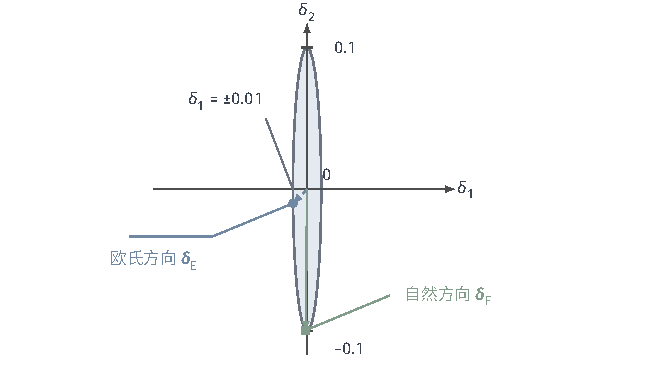
\includegraphics[width=\linewidth]{figures/02-mathematical-preliminaries-lower/01-random-variables-distributions-and-causality/tikz/information-natural-gradient-ellipse/figure.pdf}
  \caption{局部KL预算下的下降方向（解析式教学图）。灰色椭圆满足
  \(100\delta_1^2+\delta_2^2=0.01\)，对应\(\varepsilon=0.005\)。
  蓝色虚线与圆点是缩放后的欧氏方向\(\bm\delta_{\mathrm E}\)，绿色实线与方点是
  自然方向\(\bm\delta_{\mathrm F}\)；两个终点消耗相同的二次预算。
  椭圆表达分布变化代价，不是目标函数的等高线。}
  \label{fig:information-natural-gradient-ellipse}
\end{figure}

在光滑可逆重参数化下，由上一小节的矩阵和微分变换，
\[
\begin{aligned}
  \bm J\bm F_{\bm\phi}^{-1}\bm g_{\bm\phi}
  &=\bm J(\bm J^\top\bm F_{\bm\theta}\bm J)^{-1}
    \bm J^\top\bm g_{\bm\theta}\\
  &=\bm F_{\bm\theta}^{-1}\bm g_{\bm\theta}.
\end{aligned}
\]
归一化因子中的
\(\bm g_{\bm\phi}^\top\bm F_{\bm\phi}^{-1}\bm g_{\bm\phi}\)
也等于原坐标下的相应值，因此两个坐标给出同一个分布切向方向。
Bernoulli例子中，自然梯度在概率坐标为\(p(1-p)L'(p)\)，
在logit坐标为\(L'(p)\)；乘上\(\mathrm dp/\mathrm d\phi=p(1-p)\)后相同。

保持的是无穷小方向，不是任意有限离散步。
非线性坐标映射下，
\(\bm\theta(\bm\phi+\bm\delta_\phi)
=\bm\theta(\bm\phi)+\bm J\bm\delta_\phi+O(\|\bm\delta_\phi\|^2)\)，
所以分别做欧氏加法更新后的终点一般不同。
真实KL也还有\(o(\|\bm\delta\|^2)\)余项；
二次预算等于\(\varepsilon\)不保证真实KL严格不超过它。
有限步需要步长选择、真实目标或KL检查，不能由局部方向不变性直接得到全局改进。

\paragraph{奇异与近似条件下的几何更新}
\label{sec:information-singular-approximate-update}

参数冗余、退化坐标或不足的输入方向都可能使Fisher奇异。
其零空间只说明相应方向的一阶得分为零：
有时它来自完全冗余，有时如立方高斯零点，只是高阶变化未被二次型看见。
因而不能把所有零方向都理解成有限移动后分布完全不变。

回用伪逆与数值求解工具，若\(\bm g\in\operatorname{range}(\bm F)\)，
线性方程\(\bm F\bm v=\bm g\)有解，全部解为
\[
  \bm v=\bm F^\dagger\bm g+\bm z,\qquad
  \bm z\in\ker\bm F.
\]
伪逆选择当前欧氏坐标下范数最小的一个。
在得分能识别的切向商空间中，零空间分量不影响一阶分布方向，
但参数向量并不唯一，有限步的高阶效果仍可能不同。
若\(\bm g\notin\operatorname{range}(\bm F)\)，存在零方向
\(\bm z\)使\(\bm g^\top\bm z\neq0\)；
沿其下降方向任意放大仍不消耗二次预算，线性信赖域问题无下界。
此时简单写\(\bm F^\dagger\bm g\)不是原信赖域子问题的解，必须修正退化模型或约束。

阻尼使用\(\bm F+\lambda\bm I\)，其中\(\lambda>0\)，可改善病态性并保证可逆。
但它新增欧氏二次项\(\lambda\|\bm\delta\|^2\)，不是纯粹的Fisher几何：
一般坐标变化下
\[
  \bm J^\top(\bm F+\lambda\bm I)\bm J
  =\bm J^\top\bm F\bm J+\lambda\bm J^\top\bm J
  \neq\bm F_{\bm\phi}+\lambda\bm I.
\]
因此“能稳定求逆”与“保持原坐标变换性质”是不同要求。
实际计算通常求解线性系统，而不显式构造逆矩阵；
迭代容差、谱条件和矩阵近似误差也会改变得到的方向。

经验Fisher、分块或对角近似可能降低计算量，
却分别引入抽样、模型期望或跨块相关性的近似。
即使每个近似矩阵都正定，也只说明定义了某种局部内积，
不说明它等于真实分布Fisher，更不保证同样的坐标保持结论。
应区分模型下期望、真实数据下平均、固定输入权重和完整轨迹，
再说明哪一项被估计或省略。
优化收敛、模型正确性、预测校准和隐私保证还各有自己的条件；
自然梯度或KL正则不能把一种保证自动转成另一种。

\section{样本评价的总体误差}
\label{sec:information-data-dependent-evaluation}

从同一批训练样本中挑选样本损失最小的模型，再报告它的样本损失，可能偏向这批记录中的偶然低值。问题不在于总体分布改变，而在于模型选择与评价共享样本。设\(S=(Z_1,\ldots,Z_n)\)独立同分布，学习规则根据\(S\)产生随机训练模型\(W\)。对预先固定的\(w\)，样本损失是独立平均；对选出的\(W\)，模型与样本已经相互依赖。

前面的工具提供两条分析路径。比较真实联合规律与解除依赖的边缘乘积，可以控制平均评价偏差；建立同时覆盖全部候选分布的概率事件，则允许看过样本以后选择候选。两条路径的目标和量词不同，不能用平均保证替代逐样本保证。

\subsection{数据依赖下的平均评价偏差}
\label{sec:information-mi-generalization}

设可测损失\(\ell(w,Z)\in[0,1]\)，新样本\(Z\)服从与训练样本相同的总体规律，
定义
\[
  \begin{aligned}
    R(w)&=\mathbb E_Z\ell(w,Z),&
    \widehat R_S(w)&=\frac1n\sum_{i=1}^n\ell(w,Z_i),\\
    g(S,w)&=R(w)-\widehat R_S(w).
  \end{aligned}
\]
固定\(w\)时，\(\mathbb E_Sg(S,w)=0\)。
Hoeffding引理对每个中心化损失给出指数矩，再用独立性相乘，有
\[
  \mathbb E_Se^{t g(S,w)}\leq e^{t^2/(8n)},\qquad t\in\mathbb R.
\]
界不依赖\(w\)。在边缘乘积\(Q=P_S\otimes P_W\)下再对\(w\)积分，
因此\(\mathbb E_Qg=0\)，且\(g\)的方差代理为\(1/(4n)\)。
真实评价使用联合分布\(P=P_{S,W}\)，换测度的代价正是
\[
  D_{\mathrm{KL}}(P\Vert Q)=I(S;W).
\]
若互信息有限，式~\eqref{eq:information-subgaussian-change-measure}给出
\begin{equation}
  \left|\mathbb E_{S,W}\{R(W)-\widehat R_S(W)\}\right|
  \leq\sqrt{\frac{I(S;W)}{2n}}.
  \label{eq:information-mi-generalization}
\end{equation}
无限互信息时右侧无限，不提供有效保证。
这是平均有符号泛化差的绝对值，并不是
\(\mathbb E|R(W)-\widehat R_S(W)|\)，更不是逐样本高概率界。

例如算法只能输出\(M\)种预测器，则\(I(S;W)\leq H(W)\leq\log M\)，
平均偏差至多\(\sqrt{\log M/(2n)}\)。若算法完全忽略训练样本，互信息为零，
平均有符号差也为零，但每个样本的经验风险仍会波动。
反过来，连续确定性输出可能携带无限互信息；参数维数有限本身不能保证信息有限。
在本节设定中，参与学习与评价的是同一批训练样本，因此控制量是训练模型对这批样本的依赖。若改用独立评价样本，应按新的联合规律重新计算互信息；参数个数不能代替这种依赖。

\subsection{数据依赖下的同时风险控制}
\label{sec:information-pac-bayes}

有时学习规则报告的是候选模型上的一张分布\(Q_S\)，评价量便是按这张分布平均的总体风险。为了覆盖根据样本作出的选择，我们先建立对全部允许候选分布同时成立的事件。PAC--Bayes界以见样本前固定的\(P_0\)为参考，用候选相对它的KL度量选择代价。这里的先验用于风险证明；它可以独立于任何贝叶斯生成模型。

\begin{theorem}[固定参数的基础PAC--Bayes界]
\label{thm:information-pac-bayes-basic}
在上述独立同分布样本和\([0,1]\)损失设定下，令\(P_0\)在观察\(S\)前固定，
且与\(S\)独立。对任意预先固定的\(\lambda>0\)与\(0<\delta<1\)，
以至少\(1-\delta\)的概率，同时对所有\(Q\ll P_0\)有
\begin{equation}
  \mathbb E_QR(\theta)
  \leq\mathbb E_Q\widehat R_S(\theta)
  +\frac{D_{\mathrm{KL}}(Q\Vert P_0)+\log(1/\delta)}{\lambda}
  +\frac{\lambda}{8n}.
  \label{eq:information-pac-bayes-basic}
\end{equation}
KL无限时将右侧解释为无限。
\end{theorem}
\begin{proof}
对每个固定\(\theta\)，Hoeffding引理给出
\(\mathbb E_Se^{\lambda(R(\theta)-\widehat R_S(\theta))}
\leq e^{\lambda^2/(8n)}\)。
先验独立于样本，Tonelli定理允许对同一个\(P_0\)平均：
\[
  \mathbb E_S\mathbb E_{\theta\sim P_0}
  e^{\lambda(R(\theta)-\widehat R_S(\theta))}
  \leq e^{\lambda^2/(8n)}.
\]
由Markov不等式，事件
\[
  \mathcal E=
  \left\{S:\mathbb E_{P_0}e^{\lambda(R-\widehat R_S)}
  \leq\frac{e^{\lambda^2/(8n)}}{\delta}\right\}
\]
满足\(P_S(\mathcal E)\geq1-\delta\)。
对任意固定在这个事件内的样本，实现后的函数
\(f(\theta)=\lambda(R(\theta)-\widehat R_S(\theta))\)有界。
对所有\(Q\ll P_0\)分别使用式~\eqref{eq:information-dv-lower}，得到
\[
\begin{aligned}
  \lambda\mathbb E_Q(R-\widehat R_S)
  &\leq D_{\mathrm{KL}}(Q\Vert P_0)
       +\log\mathbb E_{P_0}e^{\lambda(R-\widehat R_S)}\\
  &\leq D_{\mathrm{KL}}(Q\Vert P_0)
       +\frac{\lambda^2}{8n}+\log(1/\delta).
\end{aligned}
\]
除以\(\lambda\)即得所需结论。事件只包含先验积分，不随\(Q\)改变，
因此在事件发生后选择的数据依赖\(Q_S\)也被同时覆盖。
\end{proof}

若\(P_0\)均匀分布在预先指定的\(M\)个候选上，
选择其中一个候选的点质量\(Q\)具有KL为\(\log M\)，
便得到这\(M\)个预测器的统一风险控制。
若\(P_0\)为连续分布，单点候选通常不对它绝对连续，
不能仍把该点估计作为有限KL的候选代入。

“固定\(\lambda\)”是事件成立的条件。观察数据后逐个候选优化右侧的
\(\lambda\)，或根据同一评价样本重选先验，都超出了上述事件。
可以预设可数参数网格并分配失败概率后使用并集界，
也可以用独立样本确定先验，再对剩余评价样本条件化应用定理。
这些额外步骤不能省略。互信息界比较联合规律与边缘乘积，给出平均偏差；
此处比较候选分布与先验，给出同时风险界，两者复用换测度代数但不是同一个保证。

\section{本章小结}
\label{sec:information-theory-statistical-geometry-summary}

报警概率差、平均预测损失和记录所需的码长不能用同一个数字替代。熵回答一张规律下平均需要描述多少信息，条件熵记录已有观测后剩余的部分；比较真实规律与预测规律的对数评分，多出的代价由KL给出。互信息比较联合规律与保持相同边缘的独立乘积，因此刻画变量之间的依赖。连续记录的精度与参考测度还必须明确，微分熵的单位变化不改变KL的双分布比较。

两张分布是否接近，取决于关注的量。事件概率、核函数期望和质量位移给出不同尺度；同均值可以隐藏差异，小位移也可以跨过阈值。把差异转成期望响应时，有界性、敏感性或指数矩分别提供所需控制。把差异转成辨认下界时，则同时要求候选目标相距足够远而观测规律足够近。序贯观测还要沿实际历史累计条件信息，访问次数由环境与算法共同决定。

选择一张分布、逼近一张既定分布与配对两个固定边缘，改变的是不同未知量。收益与偏离权衡给出指数倾斜，矩约束选择相容的最大熵规律，受限表示留下后验逼近误差，耦合优化保留两侧边缘。最优分布存在并不保证有限参数能够表示它；最优耦合的存在还依赖紧性和成本的下半连续性。参数迭代只在正则满秩条件下由局部KL获得Fisher度量，有限步、奇异性和近似矩阵另有误差与边界。

样本评价要额外检查模型选择怎样使用这批样本。互信息控制平均有符号评价偏差，固定先验和参数下的PAC--Bayes界控制同时覆盖候选分布的事件；平均保证不能替代高概率保证。这样的统计结论仍固定总体生成规律。若要问主动改变原因以后结果怎样响应，第~\ref{chap:causal-inference}章还需引入干预机制与识别条件。

\chapter{因果响应}
\label{chap:causal-inference}

接受培训的人平均成绩更高，是培训提高了成绩，还是基础较好的人更愿意参加培训？
第~\ref{chap:random-variables}章已经建立条件分布与统计推断，第
~\ref{chap:information-theory-and-statistical-geometry}章进一步比较分布及其对任务的
影响。但把成绩预测得很准，仍不能回答主动安排培训以后会发生什么。后一个问题要求
说明：改变的究竟是对已有记录的筛选，还是产生记录的机制。

本章研究因果响应及生成它的结构。响应把行动与个体背景映射为结果；生成结构进一步
说明这个整体映射由哪些局部关系和机制合成。我们以处理\(T\)、结果\(Y\)与处理前
信息\(X\)为共同例子，区分给定模型的计算、数据对响应的识别，以及数据对生成结构的
推断。模型明确给定时，可以直接比较行动，也可以在得知某人的事实以后计算替代结果；
这不意味着数据已经证明该模型正确。反过来，有些平均响应可以由实验设计识别，而无须
唯一恢复每一个局部方程。

计算行动后果需要一套响应规则，它把处理值与个体背景映成结果。固定同一背景可以比较个体效应，对目标总体平均可以比较人群效应；获得某人的事实后，还要先更新对其背景的认识。完成这些模型内的计算，再检查观测、实验和机制假设是否足以确定答案。

响应规则也可以由局部生成方程逐步合成。无环结构给出求值次序，图保留各方程读取的变量；这些条件进一步支持调整与结构推断。计算、识别和估计因此有各自的输入：给定模型可算出结果，相容模型是否给出同一结果决定可识别性，有限记录则决定估计精度。

\section{因果响应的表示}
\label{sec:causal-response-representation}

设同一人可以接受或不接受某项培训，我们希望计算两种安排下的成绩。培训方案、个体背景与测量时间共同决定所比较的结果。观测回归\(\mathbb E[Y\mid T=t,X=x]\)只描述自然进入处理组的人；主动安排培训还要说明哪项生成规则被替换。响应映射将这个行动约定连同背景一起写进计算。

\subsection{原因与背景的响应表示}
\label{sec:causal-observation-generation}

比较同一人的行动后果时，需要固定两种行动共同具有的背景。用\(t\)记处理值，用\(\bm u\)记这些背景差异，例如既有能力与未测量因素；可见协变量只可能记录其中一部分。模型\(M\)给出背景分布、自然运行规则以及允许替换的规则。这里假定每套规则都确定唯一结果，局部方程如何支持这一假定将在生成结构部分证明。

\begin{definition}[因果响应与自然、行动映射]
  \label{def:causal-response-interface}
  给定背景可测空间\((\mathcal U,\mathscr U)\)及概率测度\(P_{\bm U}\)，
  自然变量的可测状态空间\(\mathcal V\)，处理空间\(\mathcal T\)和结果空间
  \(\mathcal Y\)。固定模型\(M\)提供唯一值的可测自然映射
  \(F_M:\mathcal U\to\mathcal V\)，以及每个允许行动\(a\)的唯一值可测映射
  \(F_M^a:\mathcal U\to\mathcal V\)。后者由模型指定的机制替换产生，而非任意另选函数。
  若\(a(t)\)表示把处理设为\(t\)的允许行动，\(\pi_Y\)表示取结果坐标，则
  \term{因果响应}（causal response）是映射
  \begin{equation}
    R_M:\mathcal T\times\mathcal U\longrightarrow\mathcal Y,
    \qquad
    R_M(t,\bm u)=\pi_Y\bigl(F_M^{a(t)}(\bm u)\bigr).
    \label{eq:causal-response-interface}
  \end{equation}
  本章要求\(R_M\)对乘积可测结构可测。自然变量为
  \(\bm V=F_M(\bm U)\)，行动后的变量为\(\bm V_a=F_M^a(\bm U)\)。
\end{definition}

固定\(\bm u\)时，\(t\mapsto R_M(t,\bm u)\)回答同一单位怎样响应不同处理；
让\(\bm U\)按\(P_{\bm U}\)变化，才得到总体响应分布。外生背景的各分量可以相关，
定义没有默许独立性。若采用有限维参数表示\(M_{\bm\theta}\)，参数
\(\bm\theta\)描述研究者选定的机制；修改拟合参数是在改变模型，设置\(t\)则是在一个
固定模型内行动。两种变化不能互相代替。

下面用两套二元机制计算这一区别。设背景满足
\[
  U\sim\operatorname{Bernoulli}(1/2).
\]
处理与结果均取\(0,1\)。模型甲为
\begin{equation}
  T=U,\qquad Y=U;
  \label{eq:causal-observational-equivalence-confounding}
\end{equation}
模型乙为
\begin{equation}
  T=U,\qquad Y=T.
  \label{eq:causal-observational-equivalence-effect}
\end{equation}
两者自然映射都是\(F_M(u)=(u,u)\)，从而
\[
  \begin{aligned}
    \mathbb P(T=0,Y=0)&=\mathbb P(T=1,Y=1)=\frac12,\\
    \mathbb P(T=0,Y=1)&=\mathbb P(T=1,Y=0)=0.
  \end{aligned}
\]
在甲中，处理不进入结果规则；在乙中，结果直接复制处理。若允许的行动是把处理规则
替换为常数\(t\)，保留结果规则，则
\[
  F_{M_{\text{甲}}}^{a(t)}(u)=(t,u),\qquad
  F_{M_{\text{乙}}}^{a(t)}(u)=(t,t),
\]
所以\(R_{M_{\text{甲}}}(t,u)=u\)，而
\(R_{M_{\text{乙}}}(t,u)=t\)。两模型的自然映射相同，行动映射不同；
观测记录无法仅凭样本量区分这种差异。

\subsection{机制干预下的潜在结果}
\label{sec:causal-intervention-potential-outcomes}

在二元例子中，行动直接把\(T=U\)换成\(T=t\)，并沿用原来的结果规则。这项替换就是机制干预：它规定处理如何产生，再让保留的规则使用新的处理值。相同的观测条件概率没有记录这项替换，因此干预需要单独的模型约定。

\begin{definition}[理想干预]
  \label{def:causal-intervention}
  对给定模型的处理变量\(T\)作\term{干预}（intervention）
  \(\operatorname{do}(T=t)\)，表示删除自然生成\(T\)的规则，并以常量规则
  \(T=t\)替换。其余生成规则和指定的背景分布\(P_{\bm U}\)保持不变。
  由行动映射\(F_M^{a(t)}\)推前得到的分布记作
  \(P^{\operatorname{do}(T=t)}\)。
\end{definition}

“其余规则不变”不是说其余变量的取值不变。若培训改变技能，技能再影响成绩，
行动后技能和成绩都应重算。只锁住所有非处理字段再评估一个预测器，通常不是这一行动。
多变量行动同样由\(F_M^a\)表达，但模型必须说明哪些规则替换、哪些保留。

\begin{definition}[潜在结果]
  \label{def:causal-potential-outcomes}
  对明确的目标总体、处理版本和结果测量时间，\term{潜在结果}
  （potential outcome）是随机变量
  \begin{equation}
    Y(t)=R_M(t,\bm U).
    \label{eq:causal-response-potential-outcome}
  \end{equation}
  对二元处理，\((Y(0),Y(1))\)定义在同一背景概率空间上；两项分别表示同一单位
  在两种处理下的结果，而不是分别抽取两个人。
\end{definition}

可测性保证可以讨论潜在结果的概率规律。记\(\mathcal L(Z)\)为随机变量\(Z\)的分布，
则
\[
  \mathcal L(Y(t))
  =
  (R_M(t,\cdot))_{\#}P_{\bm U}
  =
  \mathcal L(Y\mid\operatorname{do}(T=t)).
\]
符号\(\#\)表示第~\ref{sec:rv-pushforward}节的分布推前。这里的
\(\operatorname{do}\)标记修改后的模型，不是对自然事件\(T=t\)作普通条件化。
潜在结果聚焦所选行动下的输出；仅有一张潜在结果表，并不自动给出其他变量的完整
生成机制\scite{math-hernan2020whatif}

观察条件分布\(p(y\mid T=t)\)会筛选自然规则恰好给出处理\(t\)的单位，因而同时
包含处理作用和进入处理组的选择。在上面两套机制中，都有
\[
  \mathbb P(Y=1\mid T=1)=1,\qquad
  \mathbb P(Y=1\mid T=0)=0.
\]
但对甲，设定处理以后结果仍为\(U\)，故
\[
  \mathbb P(Y=1\mid\operatorname{do}(T=t))=\frac12,
  \qquad t\in\{0,1\};
\]
对乙，设定处理以后结果为\(t\)，故
\[
  \mathbb P(Y=1\mid\operatorname{do}(T=t))=t.
\]
相同的观测关联对应不同的行动后果。缺少的是关于响应机制的约束，不是更精确地估计
已经相同的两个条件概率。

固定处理值并非唯一行动。\term{随机干预}（stochastic intervention）用新的随机
规则替换处理规则，例如给定处理前信息\(X=x\)时，按\(q(t\mid x)\)安排培训。
一种明确构造是加入独立于原背景的随机量\(W\)，指定
\(T=g_q(X,W)\)，使其条件分布为\(q(\cdot\mid X)\)，再运行保留的机制。
确定性策略是新规则不再需要随机化的特例。随机化是否独立、行动可使用哪些信息，
都是干预定义的一部分；仅把某个概率因子改写为\(q\)不能保证其余现实机制未变。
局部机制成立时相应的分解公式在第~\ref{sec:causal-mechanism-composition}节建立。

\subsection{观测结果与干预响应的连接}
\label{sec:causal-response-observation-link}

一名接受培训的人的实际成绩，能否作为\(Y(1)\)的记录，取决于潜在结果所指的培训方案是否与实际执行一致。不同课程、时长和测量日期会给出不同的结果变量；先把这些条件固定，才能把记录接到相应的潜在结果上。对多名参与者，还要说明一人的处理是否会改变其他人的成绩。

\begin{definition}[处理一致性与无干扰]
  \label{def:causal-consistency-no-interference}
  对明确的处理版本，\term{一致性}（consistency）要求实际处理对应的结果满足
  \(Y=Y(T)\)几乎必然成立；特别地，
  \begin{equation}
    \begin{gathered}
      T=t\Longrightarrow Y=Y(t),\\
      \text{二元处理时，}\quad Y=TY(1)+(1-T)Y(0).
    \end{gathered}
    \label{eq:causal-consistency}
  \end{equation}
  对\(n\)个单位，无干扰要求：每个\(i\)及任意两个处理向量
  \(\bm t,\bm t'\)，只要\(t_i=t_i'\)，就有
  \(Y_i(\bm t)=Y_i(\bm t')\)几乎必然成立。因此单位\(i\)的潜在结果才可简记为
  \(Y_i(t_i)\)。
\end{definition}

一致性连接自然记录与行动响应，没有把未采取行动的结果变成可见记录。若模型给出
自然处理\(T=F_{M,T}(\bm U)\)，这一条件要求自然结果与
\(R_M(F_{M,T}(\bm U),\bm U)\)相合；不能任意拼接不相容的自然函数与响应族。
在依规则替换而构造的无环模型中，这种相合性可以逐方程检查。

无干扰则限制研究单位之间的相互作用。疫苗接种、社交网络和市场竞争中，一人的行动
可能改变他人的暴露或机会；此时\(Y_i(\bm t)\)往往依赖整个处理向量。
例如\(Y_i(\bm t)=t_i+\eta\sum_{j\ne i}t_j/(n-1)\)在
\(n>1,\eta\ne0\)时不满足无干扰。可以另行规定网络暴露、分组方案或总体处理比例，
但不能继续把只比较\(t_i\)的效应解释为所有联动后果。

通常所说的稳定单位处理值假设把处理版本唯一性和无干扰合在一起。它们与分配机制仍
须分开判断：分配机制规定\(T\)怎样依赖\(X,Y(0),Y(1)\)等量，一致性只连接实际
处理与观察结果。即使处理版本清楚且单位互不干扰，主动选择培训的人也可能具有不同
背景。响应的表示到此已建立，能否由这种选择后的观测恢复响应，是后面识别部分的问题。

\section{因果响应的比较与变化}
\label{sec:causal-response-comparison}

培训对不同人的作用可能方向相反，平均成绩也可能掩盖低分概率的变化。比较之前需要确定查询：同一人改变处理会差多少，对目标人群平均会差多少，还是结果分布某个部分会怎样移动。下面固定模型、处理版本与总体，分别给这些比较建立量；连续剂量的导数再说明当前剂量附近的小变化。

\subsection{同一背景下的响应比较}
\label{sec:causal-individual-response}

已经给定\(R_M\)时，计算同一人的两种结果只改变处理值\(t\)，背景\(\bm u\)保持不动。对实值成绩，可以直接相减；所得差值刻画这一背景下的处理作用，而不是两名不同人的成绩差。

\begin{definition}[同一背景下的响应差]
  \label{def:causal-individual-effect}
  对实值结果及允许的处理值\(t,t'\)，固定背景\(\bm u\)的响应差定义为
  \begin{equation}
    \Delta_M(t,t';\bm u)=R_M(t,\bm u)-R_M(t',\bm u).
    \label{eq:causal-individual-response-difference}
  \end{equation}
  二元处理的\term{个体处理效应}（individual treatment effect）是随机变量
  \(Y(1)-Y(0)=\Delta_M(1,0;\bm U)\)。
\end{definition}

这里的减法保持同一背景，而不是用一个处理组成员减去另一个未处理组成员。
例如\(R_M(t,u)=u+(2u-1)t\)，其中\(u\in\{0,1\}\)。对背景\(u=1\)，处理使
结果增加\(1\)；对\(u=0\)，处理使结果减少\(1\)。比较两名不同背景个体的实际
结果，还混入了基础值\(u\)的差异。

给定模型和背景时，两个响应都可以计算。但每个单位的实际记录只能包含
\(Y(T)\)，不会同时包含同一时刻的\(Y(1)\)与\(Y(0)\)。因此“个体效应有明确定义”
与“它能由该人的一次观察确定”是两件事。即使已知某人当前结果为零，仍需要机制或
关于背景的信息才能计算另一行动下的结果。

对向量结果，可以先报告各坐标差，也可以指定具有实质含义的效用函数
\(h:\mathcal Y\to\mathbb R\)，比较
\(h(R_M(t,\bm u))-h(R_M(t',\bm u))\)。对类别结果，直接相减通常没有意义，
可以比较某事件的指示量。选择\(h\)是在规定目标，不是纯粹的记号替换：
提高收入、降低风险和同时满足两项要求，可能给出不同的行动排序。

\subsection{背景总体下的响应比较}
\label{sec:causal-population-response}

如果目标是决定一项培训是否适用于指定人群，可以把该人群的背景按同一分布平均。这样得到的是总体作用，允许不同背景的个体效应互相抵消。保留完整结果分布还能看到均值没有显示的变化，例如成绩的尾部或分位数；两种报告服务于不同决策问题。

\subsubsection{总体与条件总体的平均响应比较}
\label{sec:causal-average-response}

\begin{definition}[平均处理效应]
  \label{def:causal-average-treatment-effect}
  对二元处理，假设\(Y(0),Y(1)\)都可积，\term{平均处理效应}
  （average treatment effect, ATE）定义为
  \begin{equation}
    \tau
    =
    \mathbb E[Y\mid\operatorname{do}(T=1)]
    -
    \mathbb E[Y\mid\operatorname{do}(T=0)].
    \label{eq:causal-ate-interventional}
  \end{equation}
\end{definition}

两个干预总体使用同一个\(P_{\bm U}\)。由潜在结果与干预分布的对应关系及期望线性性，
\begin{equation}
  \tau
  =\mathbb E[Y(1)-Y(0)]
  =\mathbb E[Y(1)]-\mathbb E[Y(0)].
  \label{eq:causal-ate-potential-outcomes}
\end{equation}
可积性排除了\(\infty-\infty\)这样的未定义运算。线性期望说明计算平均差只需要两个
边缘均值，并没有使同一单位的两个结果同时可见。上例若
\(\mathbb P(U=1)=\mathbb P(U=0)=1/2\)，ATE为零，但没有人的个体效应为零。

若要辨认哪些人可能受益，可以在处理前协变量\(X\)下分层。
\begin{definition}[条件平均处理效应]
  \label{def:causal-conditional-average-effect}
  设\(X\)在所比较干预下保持同一取值与含义，且两种潜在结果可积。
  \term{条件平均处理效应}（conditional average treatment effect, CATE）是
  \begin{equation}
    \tau(x)=\mathbb E[Y(1)-Y(0)\mid X=x],
    \qquad P_X\text{几乎处处}.
    \label{eq:causal-cate}
  \end{equation}
\end{definition}
它对具有相同已知特征的人平均，不等于这些人逐个具有相同效应。取
\(X=U\)时，上例的\(\tau(1)=1,\tau(0)=-1\)；若\(X\)未包含\(U\)，
条件平均仍可能掩盖层内差异。不能把处理后的技能水平直接当作这里不随行动变化的
\(X\)：按两种行动各自产生的技能筛人，通常不是比较同一条件总体。

全期望给出\(\tau=\mathbb E_X[\tau(X)]\)。若响应机制不变而目标总体从\(P_X\)
换为\(Q_X\)，且对应的条件背景规律与条件效应保持不变，新ATE为
\(\int\tau(x)Q_X(\mathrm dx)\)。这是人群权重的变化，不是机制突然发生改变；
条件效应能否跨总体保留本身仍需假设。目标总体、处理版本或测量时间改变，都应重新
标明效应的含义。

对有限处理集合\(\mathcal T\)，同样定义
\[
  \tau(t,t')=\mathbb E[Y(t)-Y(t')].
\]
若行动由处理前信息决定，则要比较整个策略。令有限动作集合为\(\mathcal A\)，
策略\(\pi(a\mid x)\)用独立的新增随机化，在给定\(X=x\)时选择动作\(a\)。
在所有潜在结果可积时，它的单步价值为
\begin{equation}
  V(\pi)=\mathbb E_X\left[
    \sum_{a\in\mathcal A}\pi(a\mid X)\mathbb E[Y(a)\mid X]
  \right].
  \label{eq:causal-policy-value}
\end{equation}
式中独立随机化保证选择动作不会额外按未观测背景筛人。确定性策略是
\(\pi\)集中于一个动作的特例。这里定义的是给定模型内的目标；多值处理需要哪些
观测覆盖、策略可使用哪些已有记录，在第~\ref{sec:causal-effect-identification}节
再检查。连续剂量也不能被当作每个精确值都具有正概率的离散组。

\subsubsection{干预结果的分布响应比较}
\label{sec:causal-distribution-response}

平均值只记录分布的一个特征。设\(U\)等概率取\(-1,1\)，
\(Y(0)=0,Y(1)=U\)，则ATE为零，但处理后从人人得到零变成两种相反结果。
若低于零代表失败，这种变化对决策显然重要。

对实值结果，定义干预分布函数与其广义分位数
\[
  F_t(y)=\mathbb P(Y(t)\leq y),\qquad
  Q_t(p)=\inf\{y:F_t(y)\geq p\},\quad 0<p<1.
\]
\(F_t(y)-F_{t'}(y)\)比较不高于阈值的概率，\(Q_t(p)-Q_{t'}(p)\)比较两个总体
处于同一分位位置的结果。后者并不是个体效应
\(Y(t)-Y(t')\)的第\(p\)分位数，因为处于两个分布相同排名的未必是同一个人。
只有额外规定跨行动的排序对应关系，才能把这种配对解释成个体变化。

也可以使用第~\ref{chap:information-theory-and-statistical-geometry}章的分布比较
尺度。总变差比较事件概率而不要求矩；采用\(p\)阶Wasserstein距离时应满足所用
空间和有限\(p\)阶矩条件；使用KL散度则须检查绝对连续性及其值是否有限。
尺度的选择服务于所关心的风险或损失，不能用一个小均值差代替所有分布都接近。

两个干预边缘即使完全已知，仍没有说明它们如何在同一背景上配对。
第~\ref{sec:causal-factual-counterfactual}节将用两张联合表说明：分布比较足以回答
部分总体问题，却不足以回答已知某人事实结果后的替代结果。

\subsection{连续处理下的局部响应变化}
\label{sec:causal-local-response}

二元处理适合比较有无行动；连续剂量还可以询问“在当前剂量附近再增加一点会怎样”。
这时回用\BookSectionRef{sec:analysis-derivatives-linear-approximation}{卷1《数学准备：计算、分析与几何》第3章“测度与分析”第3.3.2节“一阶导数与线性近似”}的局部线性近似，
但求导对象必须是固定模型、固定背景下的响应。

\begin{definition}[局部响应导数]
  \label{def:causal-local-response}
  设处理取值位于开集\(\mathcal T\subseteq\mathbb R^k\)，结果位于
  \(\mathbb R^m\)。用粗体标明向量剂量；若
  \(\bm t\mapsto R_M(\bm t,\bm u)\)在\(\bm t_0\)可微，其局部响应
  Jacobian为\(D_{\bm t}R_M(\bm t_0,\bm u)\)，满足
  \[
    R_M(\bm t_0+\bm h,\bm u)-R_M(\bm t_0,\bm u)
    =D_{\bm t}R_M(\bm t_0,\bm u)\bm h+o(\|\bm h\|).
  \]
  标量处理、标量结果时记为\(\partial_tR_M(t_0,\bm u)\)。
\end{definition}

该导数是每单位剂量的局部变化，不是任意有限剂量差。比如
\(R_M(t,u)=u+t^2\)，从\(t=1\)增加到\(1+h\)的响应差是\(2h+h^2\)，
局部导数为\(2\)。\(h\)很小时一阶项有用，但从\(1\)变到\(2\)的差为\(3\)，
不能直接用导数值\(2\)代替。离散行动没有这样的邻域，仍应使用有限差。

总体平均响应\(m(t)=\mathbb E[R_M(t,\bm U)]\)还包含积分，不能仅凭每个人的
响应可微就交换求导与期望。下面给出一个可以直接检查的充分条件。
\begin{theorem}[平均响应的求导]
  \label{thm:causal-response-differentiation}
  设\(I\)是包含\(t_0\)的开区间，\(R_M(t_0,\bm U)\)可积。若对几乎每个
  \(\bm u\)，\(R_M(\cdot,\bm u)\)在\(I\)可微，且存在非负可积函数
  \(g(\bm U)\)，使
  \[
    |\partial_tR_M(t,\bm u)|\leq g(\bm u),
    \qquad t\in I,
  \]
  则\(m\)在\(t_0\)可微，且
  \begin{equation}
    m'(t_0)=\mathbb E[\partial_tR_M(t_0,\bm U)].
    \label{eq:causal-average-response-derivative}
  \end{equation}
\end{theorem}
\begin{proof}
  对足够小的非零\(h\)，中值定理给出
  \[
    \left|
      \frac{R_M(t_0+h,\bm u)-R_M(t_0,\bm u)}{h}
    \right|\leq g(\bm u).
  \]
  因而\(R_M(t_0+h,\bm U)\)可积，且差商几乎处处收敛到
  \(\partial_tR_M(t_0,\bm U)\)。可积的\(g\)统一控制这些差商，支配收敛定理
  允许将极限移入期望，得到
  \[
    \lim_{h\to0}\frac{m(t_0+h)-m(t_0)}{h}
    =
    \mathbb E\!\left[
      \lim_{h\to0}
      \frac{R_M(t_0+h,\bm U)-R_M(t_0,\bm U)}{h}
    \right],
  \]
  即所述结论。
\end{proof}

向量处理可以在相应可积控制下逐坐标求导；若要得到完整可微性，则需足以控制
Jacobian及余项的邻域条件。上述定理把“个体可微”与“可交换积分”分开，
后者限制少量背景下异常陡峭的响应，避免其破坏总体极限。

局部因果导数也不等于观测回归斜率
\(\partial_t\mathbb E[Y\mid T=t,X=x]\)。后者随\(t\)改变的还可能是自然进入
该剂量的人群；第~\ref{sec:causal-sensitivity-ranges}节将明确计算这种偏差。
它同样不同于随机轨道的It\^o微分：这里对可设定输入作普通局部变化，背景固定；
随机轨道微分描述随时间累积的随机变化，一般不存在普通逐轨道时间导数。
因此模型的光滑性支持局部计算，却不同时保证这个导数能由观测识别或能外推到大幅行动。

\section{给定事实后的因果响应}
\label{sec:causal-counterfactual-recourse}

假设某人的处理、成绩和其他记录已经可见，我们希望判断另一行动会给他带来什么结果。此时不能重新从人群中抽取背景，因为事实已经排除了一些可能的背景。固定模型后，先由事实获得背景条件分布，再用替代行动映射同一组可能背景；反事实和行动补救都从这项条件化计算出发。

\subsection{事实条件下的反事实计算}
\label{sec:causal-factual-counterfactual}

给定事实\(\bm E=\bm e\)，所求对象是这个单位在替代行动下的条件结果。模型将自然记录与替代结果放在同一背景\(\bm U\)上，事实用于限定\(\bm U\)，行动用于改变生成规则；这两个操作需要分别保留。

\begin{definition}[给定响应模型的反事实变量]
  \label{def:causal-counterfactual}
  设模型\(M\)具有定义~\ref{def:causal-response-interface}的自然映射\(F_M\)及
  行动映射\(F_M^a\)。在同一外生背景\(\bm U\)上，\term{反事实}
  （counterfactual）变量定义为\(\bm V_a=F_M^a(\bm U)\)。
  给定实际证据\(\bm E\)后的反事实分布是\(\bm V_a\)关于该证据的条件分布，
  而不是重新按背景总体抽取一个人。
\end{definition}

事实证据可来自自然变量的一部分，也可包括带噪测量；后一情形把测量随机性一并纳入
背景，使证据的生成规则明确。反事实计算通常称为“溯因、干预、预测”：
溯因由事实得到背景条件分布，干预切换到允许的行动映射，预测将同一个背景条件分布
推到结果空间。这里的溯因是给定模型内的条件化，并不是由一条记录证明模型正确。

设空间允许选取正则条件分布
\(P_{\bm U\mid\bm E=\bm e}\)，例如本章常用的标准Borel空间。回用第
~\ref{sec:rv-conditional-distribution}节，对任意可测集合\(B\)，三步合成为
\begin{equation}
  \begin{aligned}
    \mathbb P(\bm V_a\in B\mid\bm E=\bm e)
    &=
    \bigl((F_M^a)_{\#}
      P_{\bm U\mid\bm E=\bm e}\bigr)(B)\\
    &=
    \int\mathbb I\{F_M^a(\bm u)\in B\}
      P_{\bm U\mid\bm E=\bm e}(\mathrm d\bm u).
  \end{aligned}
  \label{eq:causal-counterfactual-pushforward}
\end{equation}
式中事实只进入背景条件分布，行动只进入映射。连续证据点通常概率为零，等式按所选
正则条件分布版本理解，只保证对证据分布几乎处处的\(\bm e\)成立。在一个指定的
零概率证据点上报告数值，还需要选定版本或连续性等额外结构；积分恒等式本身不能
唯一规定每个点的条件值。

考虑已经明确给定的教学模型
\begin{equation}
  X=U_X,\qquad
  T=f_T(X,U_T),\qquad
  Y=2X+3T+U_Y.
  \label{eq:causal-counterfactual-linear-example}
\end{equation}
它直接提供自然映射及替换处理规则后的映射。某人的事实为
\(X=2,T=0,Y=5\)，于是
\[
  U_Y=5-2\times2-3\times0=1.
\]
保持该人的\(X,U_Y\)不变，把处理设为\(1\)，得到
\[
  Y_{T\leftarrow1}=2\times2+3\times1+1=8.
\]
差值\(3\)来自给定结果规则中的处理作用。事实不必确定全部背景，例如可能仍不知道
\(U_T\)；只要未确定部分不影响本次行动后的结果，仍能得到这个点值。
若结果规则不确定，或未确定的背景继续进入结果，则应给出条件分布或范围。

\begin{example}[两点背景后验的反事实推前]
  \label{ex:causal-two-point-background-posterior}
  令背景类型\(U\in\{u_{\mathrm L},u_{\mathrm H}\}\)先验概率各为\(1/2\)。
  事实中观察到二元信号\(S=1\)，且模型规定
  \[
    \mathbb P(S=1\mid U=u_{\mathrm H})=\frac34,\qquad
    \mathbb P(S=1\mid U=u_{\mathrm L})=\frac14.
  \]
  因而\(\mathbb P(S=1)=\frac12(\frac34+\frac14)=\frac12\)，Bayes公式给出
  \[
    \mathbb P(U=u_{\mathrm H}\mid S=1)=\frac34,\qquad
    \mathbb P(U=u_{\mathrm L}\mid S=1)=\frac14.
  \]
  若行动\(a\)下的结果在两类背景中分别为
  \(F_{M,Y}^a(u_{\mathrm L})=2,F_{M,Y}^a(u_{\mathrm H})=6\)，则
  \[
    \mathcal L(Y_a\mid S=1)=\frac14\delta_2+\frac34\delta_6,\qquad
    \mathbb E[Y_a\mid S=1]=\frac14\,2+\frac34\,6=5.
  \]
  忽略事实而按先验重新抽取背景，得到总体干预分布
  \(\frac12\delta_2+\frac12\delta_6\)，均值为\(4\)。
  两个答案使用同一行动映射，只是反事实计算保留了事实提供的背景信息。
\end{example}

这个例子也可放回完整背景接口：另加独立测量随机量生成信号\(S\)，行动结果只依赖
类型\(U\)，于是积分掉测量背景就得到上面的两点后验。未知背景不必被硬选成某一类。

图~\ref{fig:causal-abduction-intervention-prediction}并列展示这两条推前路径：条件反事实保留事实形成的后验，总体干预沿用背景先验。

\begin{figure*}[htbp]
  \centering
  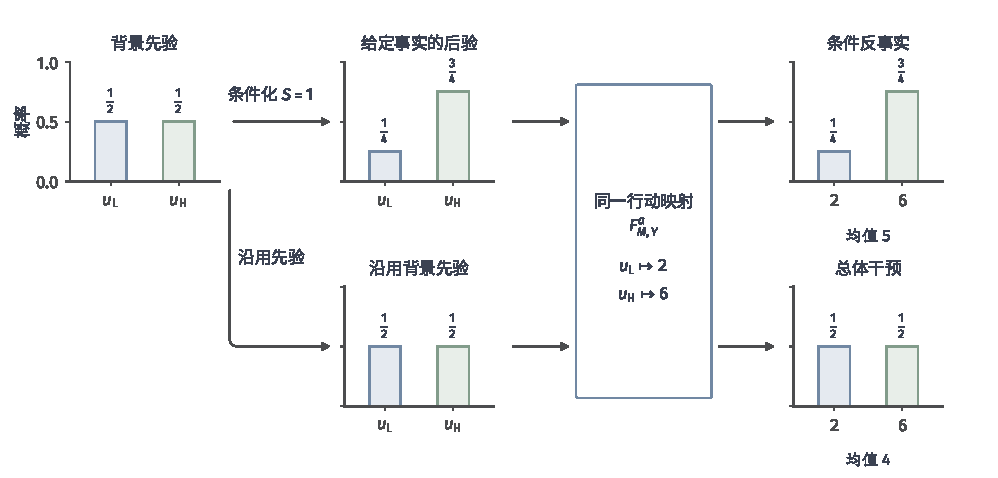
\includegraphics[width=169mm]{figures/02-mathematical-preliminaries-lower/01-random-variables-distributions-and-causality/matplotlib/causal-two-point-pushforwards/figure.pdf}
  \caption{同一行动映射下的条件反事实与总体干预。背景$u_{\mathrm L},u_{\mathrm H}$的先验概率各为$1/2$，
  事实$S=1$将两者的后验概率更新为$1/4,3/4$；行动映射分别给出结果$2,6$。
  保留后验得到条件均值$5$，沿用先验得到总体干预均值$4$。
  概率柱使用共同的零基线与比例尺；溯因是给定模型内的条件化，不证明结构假设本身有效。}
  \label{fig:causal-abduction-intervention-prediction}
\end{figure*}


还有一种更深的歧义：即使知道两种行动各自的总体分布，也未必知道同一个人的两个
结果怎样配对。设两种干预结果均为\(\operatorname{Bernoulli}(1/2)\)。
模型甲令一半单位满足\((Y(0),Y(1))=(0,0)\)，另一半满足\((1,1)\)；
模型乙令两类单位分别满足\((0,1)\)和\((1,0)\)。甲的个体效应恒为零，
乙的个体效应等概率取\(1,-1\)，而两模型的ATE都为零。

图~\ref{fig:causal-cross-world-couplings}给出了对应的联合概率表。用定义
~\ref{def:information-coupling}的语言，两者是相同边缘的不同耦合。
已知\(Y(0)=0\)时，甲给\(Y(1)=0\)，乙给\(Y(1)=1\)。在独立随机分配处理
的事实世界里，观察到\(T=0,Y=0\)就能形成这项对照：两个模型仍给出不同反事实。

\begin{figure}[htbp]
  \centering
  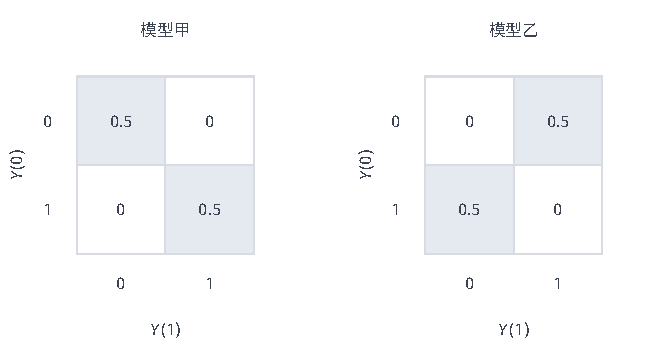
\includegraphics[width=\linewidth]{figures/02-mathematical-preliminaries-lower/01-random-variables-distributions-and-causality/tikz/causal-cross-world-couplings/figure.pdf}
  \caption{相同干预边缘的两种跨世界配对。行对应\(Y(0)\)，列对应\(Y(1)\)，格内
  数字为联合概率；每张表的行和、列和均为\(1/2\)。甲的个体效应恒为零，乙的个体
  效应等概率取\(1,-1\)，两者ATE均为零。这是相容机制的教学构造，不是随机试验
  直接观察到的潜在结果联合表。}
  \label{fig:causal-cross-world-couplings}
\end{figure}

两套配对连完整随机试验的两组边缘也无法区分。要回答条件个体反事实，还需要关于
跨世界联合结构的机制限制，或具有适当稳定性、时间和携带效应假设的重复干预资料；
否则应保留相容范围。模型明确给定时可以用式
~\eqref{eq:causal-counterfactual-pushforward}计算，数据是否足以确定这套模型则是
第~\ref{sec:causal-effect-identification}节的另一个问题。

\subsection{目标约束下的行动补救}
\label{sec:causal-action-recourse}

反事实计算还可以反过来服务于行动选择：怎样以尽量低的代价，让同一个人的决策
达到目标？先区分两种看似相近的操作。对预测器\(\widehat y=f(x,t)\)，输入替换给出
\[
  f(x,1)-f(x,0).
\]
这只是已训练函数对字段变化的响应。若现实培训提高技能、同时占用工作时间，那么
只改“是否培训”一列而锁住技能和时间，通常不是任何可实施的行动结果。

\begin{definition}[因果行动补救]
  \label{def:causal-recourse}
  给定事实证据、可实施行动集合\(\mathcal A(x)\)、响应模型、行动成本\(c(a;x)\)
  与目标决策集合\(G\)，\term{行动补救}（algorithmic recourse）寻找能够使行动后
  的决策落入\(G\)的可行行动。因果行动补救用同一背景下的干预状态
  \(\bm V_a=F_M^a(\bm U)\)评价成功条件，并按机制重算所有受行动影响的状态。
\end{definition}

令\(d\)为最终决策规则。若事实唯一确定背景\(\bm u\)，优化形式为
\begin{equation}
  \min_{a\in\mathcal A(x)}c(a;x)
  \quad\text{使得}\quad d(F_M^a(\bm u))\in G.
  \label{eq:causal-recourse-objective}
\end{equation}
可行集合规定实际允许做什么，成本规定如何比较行动，成功约束规定要得到何种决策。
它们对应\BookChapterRef{chap:optimization}{卷1《数学准备：计算、分析与几何》第4章“最优化”}的约束优化接口，但不能只根据一个距离函数
代替全部三项。低输入距离不等于低行动成本；不可改变属性也不应成为行动建议。
若可行集合为空，应报告无法在当前约束下补救，而不是输出一个不可执行的最近点。

多数事实只能给出背景条件分布。给定可容许失败概率\(\alpha\in[0,1]\)，可以采用
概率型约束
\begin{equation}
  \mathbb P\bigl(d(F_M^a(\bm U))\in G\mid\bm E=\bm e\bigr)
  \geq1-\alpha.
  \label{eq:causal-recourse-probability}
\end{equation}
若背景空间为Polish空间，且所用条件分布版本是其Borel概率测度，可以取该条件分布的支持
\[
  \mathcal S_{\bm e}
  =\operatorname{supp}P_{\bm U\mid\bm E=\bm e}.
\]
要求
\begin{equation}
  d(F_M^a(\bm u))\in G,\qquad \bm u\in\mathcal S_{\bm e},
  \label{eq:causal-recourse-robust}
\end{equation}
这给出支持上的最坏情形保证。该支持具有条件概率一，因此支持上的逐点成功蕴含概率一成功；它还约束支持中
零概率点上的模型取值，因而可能严格更强。一般可测空间没有默认的拓扑支持，
此时应明确给出候选背景集合。若要由该集合上的逐点保证推出概率一成功，
还须要求该集合具有条件概率一。

两点后验例子可以直接比较这些条件。若目标是\(Y_a\geq5\)，行动\(a\)的后验成功
概率为\(3/4\)，因此在\(\alpha=1/4\)时满足概率约束；但低类型背景的结果为\(2\)，
不能满足支持上的最坏情形保证。只挑高类型作为“代表背景”会漏掉这项风险。

补救也有时间和多人联动的边界。许多人同时接受建议可能改变价格、名额或审核规则；
决策系统更新后，原建议未必仍有效；资源竞争也可能使原先逐人可行的行动无法共同
执行。因此当前模型中存在一个成功行动，不等于建议已经通过现实可行性、持久性
或公平性验证。

\subsection{目标属性干预下的公平补救}
\label{sec:causal-fair-recourse}

设行动已经能改变当前决策，我们还可能要求这种成功不依赖某项受保护属性。检验这一要求，需要在同一背景下替换属性，并重新计算属性改变所影响的其他变量。哪些影响应被排除是一项规范选择；给定这个选择之后，模型才能定义需要比较的反事实结果。

令受保护属性为\(A\)，事实证据为\((X=x,A=a)\)。本小节的\(X\)泛指用于推断
背景的其他事实，可能包含属性的后继变量；它不再具有CATE中“处理前且保持不变”
的自动含义。事实中给定\(X=x\)，并不要求替代属性世界的\(X\)仍等于\(x\)。
\begin{definition}[反事实公平]
  \label{def:causal-counterfactual-fairness}
  在给定响应模型与预测规则下，\term{反事实公平}（counterfactual fairness）
  要求：对每个允许的替代属性\(a'\)和每个可测预测值集合\(B\)，以下等式对事实
  证据分布几乎处处的\((x,a)\)成立：
  \begin{equation}
    \begin{aligned}
      &\mathbb P(\widehat Y_{A\leftarrow a}\in B\mid X=x,A=a)\\
      &\qquad=
      \mathbb P(\widehat Y_{A\leftarrow a'}\in B\mid X=x,A=a).
    \end{aligned}
    \label{eq:causal-counterfactual-fairness}
  \end{equation}
  两个属性世界均使用同一个事实背景条件分布，并重新计算由属性影响的状态及预测。
\end{definition}

等式右侧仍以事实\(A=a\)为条件，而不是改用另一群人的证据\(A=a'\)。
只在输入表中替换\(A\)并固定其全部后继变量，检验的是另一个对象。属性干预在这里
是明确模型下的比较操作，也不表示应建议个人改变该属性。

把公平条件加入补救时，为避免与属性值混淆，记补救行动为\(b\)。
要求模型已经规定联合行动映射\(F_M^{b,A\leftarrow a'}\)：对每个属性世界，
保留同一个可比较的行动\(b\)，不对该世界偷偷重新选择更有利的行动。行动与属性
替换须互相兼容，且所比较世界中行动的可实施含义应明确。定义
\[
  \Pi_b^{a'}(B;x,a)
  =
  \mathbb P\bigl(
    d(F_M^{b,A\leftarrow a'}(\bm U))\in B
    \mid X=x,A=a
  \bigr).
\]
一种公平约束补救问题是
\begin{equation}
  \begin{aligned}
    \min_{b\in\mathcal A(x,a)}\quad &c(b;x,a)\\
    \text{使得}\quad
    &\Pi_b^a(G;x,a)\geq1-\alpha,\\
    &\Pi_b^{a'}(\cdot;x,a)=\Pi_b^a(\cdot;x,a)
      \quad\text{对每个允许的 }a'.
  \end{aligned}
  \label{eq:causal-fair-recourse-objective}
\end{equation}
第一项约束要求成功，第二项约束要求同背景的决策分布不随属性改变。也可以另选近似
公平或成本公平目标，但那会改变问题，不能把它们当作上述等式的自动结果。

\begin{example}[成功行动未必满足公平约束]
  \label{ex:causal-fair-recourse}
  设\(A\in\{0,1\}\)，自然培训量为\(B=0\)，资格分数与二元决策规则为
  \[
    K=U+A+B,\qquad d=\mathbb I\{K-2A\geq2\}.
  \]
  可行行动是把培训量设为\(b\in[0,3]\)，成本为\(c(b)=b\)，目标为\(d=1\)。
  已知事实\(A=0,B=0,K=1\)，于是\(U=1\)。在两个属性世界中施加同一行动，
  必须重算\(K\)，得到
  \[
    K_{b,A\leftarrow a'}=1+a'+b,\qquad
    d_{b,A\leftarrow a'}=\mathbb I\{1+b-a'\geq2\}.
  \]
  只要求事实属性下成功时，最小行动为\(b=1\)。但此时\(a'=0\)给决策\(1\)，
  \(a'=1\)给决策\(0\)，并不公平。若同时要求两个属性世界的二元决策相同且
  成功，则必须\(b\geq2\)，故最优行动为\(b=2\)。不行动时两个世界都失败，
  虽然决策相同，却不满足补救目标。
\end{example}

此例检验的是二元决策，不是内部实值分数\(K-2A\)；后者在两个属性世界中始终
相差\(1\)，任何培训量都不能让分数分布相同。公平对象、允许行动及预算都会影响
可行性。对一个已知个体成立的约束，也不自动保证面向所有人的推荐规则公平；
后者还需规定推荐怎样依赖事实，并对其目标人群几乎处处检验。

这些等式均以给定模型为条件。第~\ref{sec:causal-factual-counterfactual}节的
跨世界配对已经说明，相同干预边缘也可能给出不同条件反事实；由观测拟合出一套
生成规则，不等于公平或补救结论已被唯一识别。若多个模型与证据相容，应在该模型类
上报告结论范围。哪些属性或路径属于不应进入决策的因素，则是另需论证的规范选择。
\BookChapterRef{chap:trust-fairness}{卷3《基础、理论与可信性》第13章“公平性”}与
\BookChapterRef{chap:trust-interpretability}{卷3《基础、理论与可信性》第15章“可解释性”}
继续讨论公平要求、解释和补救的应用及现实验证边界。

\section{因果响应的推断}
\label{sec:causal-effect-identification}

响应计算已经给出每套模型的答案，实际研究却可能不知道哪套模型产生了记录。现在固定可观测分布和机制假设，保留与两者相容的模型，再检查这些模型是否给出同一个响应目标。定义~\ref{def:statistics-identifiability}中的可识别性在这里比较完整生成机制；若目标已被唯一确定，有限样本估计仍会留下统计误差。

记\(P_{\mathrm{obs}}^M\)为模型\(M\)在已声明观测制度下给出的可观测分布，
\(\tau(M)\)为目标。在允许模型类中，若
\[
  P_{\mathrm{obs}}^{M_1}=P_{\mathrm{obs}}^{M_2}
  \quad\Longrightarrow\quad \tau(M_1)=\tau(M_2),
\]
就称该目标\term{可识别}（identifiable）。可观测分布可以包括已完成的试验资料，
不必只包括自然观察。目标可识别也不要求模型每个组成部分都唯一确定。

这是总体层面的唯一性，须与有限样本估计、数值计算区分。估计用样本逼近总体量，
计算求出给定表达式或优化问题的答案。一个算法可以精确拟合全部观测条件分布，
却仍无法区分本章开头的两套机制；反过来，目标已有识别式，也不表示样本够多或
数值算法已经稳定。

\subsection{响应目标的点识别}
\label{sec:causal-point-identification}

目标处理下的结果只在实际得到该处理的人身上可见。要用他们代表目标总体，需要限制处理选择与潜在结果之间的关系。随机分配直接建立这种关系；观察研究可以在处理前信息充分时，用条件交换性支持调整。下面先在潜在结果语言中证明相应等式，再由图条件解释某些调整集合为何成立。

\subsubsection{随机分配下的边缘识别}
\label{sec:causal-randomized-identification}

若处理由独立随机装置分配，且两种处理都有正概率，则
\((Y(0),Y(1))\perp T\)。结合一致性，对任意可测集合\(B\)及
\(t\in\{0,1\}\)，有
\begin{equation}
  \mathbb P(Y(t)\in B)
  =
  \mathbb P(Y(t)\in B\mid T=t)
  =
  \mathbb P(Y\in B\mid T=t).
  \label{eq:causal-randomization-marginal-distribution}
\end{equation}
第一个等号来自随机分配，第二个来自实际处理与潜在结果的一致性；正概率保证右侧
有相应处理组。结果可积时，同一论证给出
\[
  \mathbb E[Y(t)]
  =\mathbb E[Y(t)\mid T=t]
  =\mathbb E[Y\mid T=t],
\]
所以两组均值差识别ATE。

式~\eqref{eq:causal-randomization-marginal-distribution}识别的是每个潜在结果的
完整边缘，不是\((Y(0),Y(1))\)的联合分布。第
~\ref{sec:causal-factual-counterfactual}节的两套配对因此仍与随机试验相容。
若实际分析存在失访、不依从、处理溢出或随机化后的样本筛选，应按真实目标重新检查
独立性和一致性。例如随机分配的邀请不等于实际参加培训，按参加者重新分组不会自动
继承原随机化。

\subsubsection{条件交换下的调整识别}
\label{sec:causal-adjustment-identification}

观察研究不能随意重排处理，但可以尝试用处理前\(X\)解释分配差异。这里的\(X\)
须在所比较处理下保持同一取值和含义，否则两组不再按共同背景分层。
\begin{definition}[条件交换性]
  \label{def:causal-conditional-exchangeability}
  对二元处理，\term{条件交换性}（conditional exchangeability）要求
  \begin{equation}
    (Y(0),Y(1))\perp T\mid X.
    \label{eq:causal-conditional-exchangeability}
  \end{equation}
\end{definition}
直观上，固定\(X\)后，进入处理组不再额外透露潜在结果的信息；例如\(X\)已经
包含需要控制的共同背景。这不同于概率论中样本序列在重排下分布不变的可交换性。
它涉及不能同时观察的结果，不能凭处理预测准确率或结果拟合误差验证。对单个边缘
目标，只需相应的\(Y(t)\perp T\mid X\)；上式是同时表达两种处理可比性的较强条件。

\begin{definition}[二元处理的支持重叠]
  \label{def:causal-overlap}
  记倾向概率为\(e(x)=\mathbb P(T=1\mid X=x)\)。对需要比较两种处理的目标总体，
  \term{支持重叠}（overlap），也称\term{正值性}（positivity），要求
  \begin{equation}
    0<e(x)<1,\qquad P_X\text{几乎处处}.
    \label{eq:causal-overlap}
  \end{equation}
\end{definition}
交换性解释参照人群为何可比，支持重叠保证参照确实存在。若某类人必然接受处理，
即使愿意假设其未处理潜在结果与分配条件独立，也没有该类人的未处理记录可用。

正值性随目标而定。识别\(\mathbb E[Y(1)]\)只需目标总体几乎处处有\(e(x)>0\)，
识别\(\mathbb E[Y(0)]\)只需\(e(x)<1\)，ATE才同时需要两侧条件。
对目标策略，只有它会使用的背景与行动组合需要被观测支持覆盖；目标总体以外的
背景和策略从不采取的行动不在要求内。若另换目标总体，其背景支持和跨总体条件
响应的可比性也要重新检查。

假设一致性、条件交换性、所需支持及潜在结果可积性成立。全期望先给出
\[
  \mathbb E[Y(t)]
  =\mathbb E_X[\mathbb E[Y(t)\mid X]].
\]
交换性允许在内层加入处理条件：
\[
  \mathbb E[Y(t)\mid X]
  =\mathbb E[Y(t)\mid T=t,X].
\]
正值性保证右侧在目标所需的背景上由相应处理组定义，一致性再将\(Y(t)\)换成
观察结果，得到调整公式
\begin{equation}
  \mathbb E[Y(t)]
  =\mathbb E_X[\mathbb E[Y\mid T=t,X]].
  \label{eq:causal-g-formula}
\end{equation}
令\(\mu_t(x)=\mathbb E[Y\mid T=t,X=x]\)，两式相减便有
\begin{equation}
  \tau=\mathbb E_X[\mu_1(X)-\mu_0(X)].
  \label{eq:causal-ate-adjustment}
\end{equation}
若把结果换成事件指示量，同样可以识别各干预边缘的事件概率。

同一目标还有逆概率表示。对处理组，由条件期望
\[
  \begin{aligned}
    \mathbb E\left[\frac{TY}{e(X)}\middle|X\right]
    &=
    \frac{\mathbb P(T=1\mid X)}{e(X)}
      \mathbb E[Y\mid T=1,X]\\
    &=\mu_1(X).
  \end{aligned}
\]
未处理组同理满足
\[
  \mathbb E\left[\frac{(1-T)Y}{1-e(X)}\middle|X\right]
  =\mu_0(X).
\]
可积性使这些期望存在，再取总体期望得到
\begin{equation}
  \tau=\mathbb E\left[
    \frac{TY}{e(X)}-\frac{(1-T)Y}{1-e(X)}
  \right].
  \label{eq:causal-ipw-identification}
\end{equation}
条件均值法先在层内比较再按总体平均；加权法给较少进入某处理的单位更大权重。
两者是同一识别关系的表示，不是两套彼此替代的因果假设。

下面把分配差异具体算出来。设\(X\in\{0,1\}\)表示处理前风险，
\(\mathbb P(X=1)=1/2\)，且
\[
  e(1)=0.8,\qquad e(0)=0.2.
\]
给定\(X\)后假设交换性成立，潜在结果均值取教学数值
\[
  \begin{array}{c|cc}
    &X=0&X=1\\ \hline
    \mathbb E[Y(0)\mid X]&0.1&0.5\\
    \mathbb E[Y(1)\mid X]&0.3&0.7
  \end{array}
\]
两层效应都为\(0.2\)，所以
\[
  \tau=\tfrac12(0.3-0.1)+\tfrac12(0.7-0.5)=0.2.
\]
自然处理中\(\mathbb P(T=1)=\tfrac12(0.8+0.2)=1/2\)，Bayes公式给出
\[
  \mathbb P(X=1\mid T=1)=0.8,\qquad
  \mathbb P(X=1\mid T=0)=0.2.
\]
于是观察到的两组均值为
\[
  \begin{aligned}
    \mathbb E[Y\mid T=1]&=0.8\times0.7+0.2\times0.3=0.62,\\
    \mathbb E[Y\mid T=0]&=0.2\times0.5+0.8\times0.1=0.18.
  \end{aligned}
\]
观测差为\(0.44\)，大于调整后的\(0.20\)，因为处理组中基础结果较高的高风险者
更多。按共同的\(P_X\)重新平均就恢复了所定义的总体效应。

这也说明三项假设各管什么。一致性连接观测和潜在结果，交换性允许同层比较，重叠
让每层都有所需的处理记录。遗漏未记录的病情可能破坏交换性；若\(e(1)=1\)，
高风险层的未处理结果完全缺失。相反，\(e(1)\)很接近但未等于\(1\)时，点识别
仍成立，只是有限样本中权重可能很大。选择哪些协变量足以支持调整，需要领域知识
或结构证书；第~\ref{sec:causal-backdoor-selection}节在建立图语义后给出一种
充分准则，这里并未假定该准则已经被验证。

\subsection{响应目标的部分识别}
\label{sec:causal-partial-identification-sensitivity}

若不愿接受完整交换性，或目标行动落入无数据的区域，仍可询问现有信息排除了哪些
答案。这就是\term{部分识别}（partial identification）：保留所有相容机制给出的
目标值，不用一个未经支持的点掩盖机制歧义。
\begin{definition}[识别集合]
  \label{def:causal-identified-set}
  设\(\mathcal M(P_{\mathrm{obs}})\)是与可观测分布及已声明假设相容的模型集合，
  目标为\(\tau(M)\)。其\term{识别集合}（identified set）是
  \begin{equation}
    \mathcal I(P_{\mathrm{obs}})
    =\{\tau(M):M\in\mathcal M(P_{\mathrm{obs}})\}.
    \label{eq:causal-identified-set}
  \end{equation}
\end{definition}
相容类为空意味着假设与观测不相容，并不是“目标取空值”。以下讨论相容类非空的
情形。一般识别集合可能由分离的点或区间组成；下确界和上确界只给区间包络，
不能保证包络内每个值可达。只有另外证明中间值可达，才能把整个区间称为识别集合。

\subsubsection{结果约束下的效应界}
\label{sec:causal-outcome-bounds}

先只保留一致性及结果范围\(0\leq Y(t)\leq1\)，不假设交换性。二元处理下，
\[
  \begin{aligned}
    \mathbb E[Y(1)]
    &=\mathbb E[TY(1)]+\mathbb E[(1-T)Y(1)]\\
    &=\mathbb E[TY]+\mathbb E[(1-T)Y(1)].
  \end{aligned}
\]
第一项已经观察到；第二项是未处理者接受处理后的结果。由范围约束，
\[
  0\leq\mathbb E[(1-T)Y(1)]\leq\mathbb P(T=0),
\]
所以
\begin{equation}
  \mathbb E[TY]\leq\mathbb E[Y(1)]
  \leq\mathbb E[TY]+\mathbb P(T=0).
  \label{eq:causal-bounded-outcome-y1}
\end{equation}
对另一处理，同样将
\(\mathbb E[Y(0)]=\mathbb E[(1-T)Y]+\mathbb E[TY(0)]\)分成可见与缺失部分，
得到
\begin{equation}
  \mathbb E[(1-T)Y]\leq\mathbb E[Y(0)]
  \leq\mathbb E[(1-T)Y]+\mathbb P(T=1).
  \label{eq:causal-bounded-outcome-y0}
\end{equation}
用第一式下端减第二式上端，反向组合得到上端：
\begin{equation}
  \begin{aligned}
    &\mathbb E[TY]-\mathbb E[(1-T)Y]-\mathbb P(T=1)
      \leq\tau\\
    &\qquad\leq
      \mathbb E[TY]+\mathbb P(T=0)-\mathbb E[(1-T)Y].
  \end{aligned}
  \label{eq:causal-manski-ate-bounds}
\end{equation}

界宽并不一定表示推导粗糙；它可能正是资料缺失造成的。
\begin{definition}[相容机制类中的锐界]
  \label{def:causal-sharp-bounds}
  对非空相容类\(\mathcal M(P_{\mathrm{obs}})\)与实值目标，若下界与上界分别等于
  \(\inf_{M\in\mathcal M}\tau(M)\)及\(\sup_{M\in\mathcal M}\tau(M)\)，就称为
  该机制类中的\term{锐界}（sharp bounds）。端点可以达到，也可以仅由相容
  机制序列任意逼近。
\end{definition}

式~\eqref{eq:causal-manski-ate-bounds}在当前不受其他限制的机制类中是锐的。
要达到下界，保持所有实际记录不变，令未处理者缺失的\(Y(1)=0\)，已处理者
缺失的\(Y(0)=1\)。要达到上界，则把这两类缺失结果分别设为\(1\)和\(0\)。
两种构造都满足一致性和结果范围，也不改变\(P_{\mathrm{obs}}\)。

中间值也可构造。独立抽取一个概率为\(\lambda\)的二元背景标记，按该标记选择
上端构造，否则选择下端构造；事实记录不变，只切换缺失结果的赋值。
混合机制的效应为\(\lambda\tau_{\mathrm{up}}+(1-\lambda)\tau_{\mathrm{low}}\)。
让\(\lambda\)遍历\([0,1]\)，便得到整个区间。这证明宽度不是代数松弛造成的。
若再要求个体单调性、平滑函数或特定跨世界结构，上述赋值可能不再允许，
锐界必须在新的模型类中重新计算。

\subsubsection{支持缺口下的效应与策略界}
\label{sec:causal-support-policy-bounds}

现在假设条件交换性可信，但双侧重叠只在协变量区域\(\mathcal O\)成立。用
\(\mathcal N\)表示目标总体中缺少某种处理的区域，两者不交且覆盖目标总体。
结果仍在\([0,1]\)时，条件效应\(\tau(x)\in[-1,1]\)，故
\[
  \tau=
  \mathbb E[\tau(X)\mathbb I\{X\in\mathcal O\}]
  +\mathbb E[\tau(X)\mathbb I\{X\in\mathcal N\}].
\]
第一项由调整式识别，第二项只能先按范围控制，得到
\begin{equation}
  \begin{aligned}
    &\mathbb E[\tau(X)\mathbb I\{X\in\mathcal O\}]
      -\mathbb P(X\in\mathcal N)\leq\tau\\
    &\qquad\leq
      \mathbb E[\tau(X)\mathbb I\{X\in\mathcal O\}]
      +\mathbb P(X\in\mathcal N).
  \end{aligned}
  \label{eq:causal-overlap-gap-bounds}
\end{equation}
这是一组有效界，未声称总是锐界；缺口区域中若仍观察到一种处理的结果，
利用这一侧均值还可能收紧。限制目标人群到\(\mathcal O\)可以点识别重叠人群效应，
但已经改变了目标总体。假设缺口内效应与邻近区域平滑、同号或落在更小范围，也能
收紧答案，却都是额外外推条件，不能由已覆盖部分的拟合优度证明。

单步策略评价需要的支持可以更少。沿用式~\eqref{eq:causal-policy-value}的有限
动作集合及目标策略\(\pi\)，记日志动作概率为
\(e_a(x)=\mathbb P(T=a\mid X=x)\)。假设对所有动作，
\(L\leq Y(a)\leq H\)，且一致性和给定\(X\)的交换性成立。若目标覆盖条件为
\[
  \pi(a\mid x)>0\quad\Longrightarrow\quad e_a(x)>0
\]
并在目标总体中几乎处处成立，则
\[
  \begin{aligned}
    \mathbb E\left[\frac{\pi(T\mid X)}{e_T(X)}Y\middle|X\right]
    &=
    \sum_{\substack{a\in\mathcal A\\e_a(X)>0}}
      e_a(X)\frac{\pi(a\mid X)}{e_a(X)}
      \mathbb E[Y\mid T=a,X]\\
    &=
    \sum_{a\in\mathcal A}\pi(a\mid X)\mathbb E[Y(a)\mid X].
  \end{aligned}
\]
对\(X\)取期望，得到
\begin{equation}
  V(\pi)=\mathbb E\left[\frac{\pi(T\mid X)}{e_T(X)}Y\right].
  \label{eq:causal-policy-value-weighting}
\end{equation}
这是第~\ref{sec:rv-change-measure}节换测度的一个因果用途：改变动作分配，
保留给定背景与动作的结果机制。权重只在日志实际可能选择的动作上求值，
覆盖条件使其余动作的目标概率为零，无须引入\(0/0\)约定。

覆盖失败时，记目标策略落入缺口的概率质量及已识别贡献为
\[
  \begin{aligned}
    r&=\mathbb E_X\left[\sum_{a:e_a(X)=0}\pi(a\mid X)\right],\\
    K&=\mathbb E_X\left[
      \sum_{a:e_a(X)>0}\pi(a\mid X)\mathbb E[Y\mid T=a,X]
    \right].
  \end{aligned}
\]
缺口部分的贡献在\([Lr,Hr]\)内，因而
\begin{equation}
  K+Lr\leq V(\pi)\leq K+Hr.
  \label{eq:causal-policy-value-bounds}
\end{equation}
两个策略的价值范围若完全分离，就能确定排序；若重叠，单独看边际范围未必能
判断。它们使用同一组未知潜在结果，不能把各自端点当作独立可选。
例如两策略完全相同时，无论各自的价值范围多宽，价值差都严格为零。
一般应对
\[
  V(\pi_1)-V(\pi_2)
  =
  \mathbb E_X\sum_a
    \bigl(\pi_1(a\mid X)-\pi_2(a\mid X)\bigr)\mathbb E[Y(a)\mid X]
\]
直接构造联合识别集合或上下界。拟合器对缺口给出的单一外推，不是额外的排序证据。

图~\ref{fig:causal-confounding-coverage}把混杂与覆盖分别数值化。左图回顾前面的
风险分层例子；右图另设结果范围为\([0,1]\)，已覆盖部分条件平均收益为\(0.6\)，
故\(K=0.6(1-r)\)。在\(r=0.2\)时，价值范围为\([0.48,0.68]\)。
宽度\(0.2\)来自缺口中的未知结果机制，不会因增加同一覆盖区域内的样本而消失。
\begin{figure*}[htbp]
  \centering
  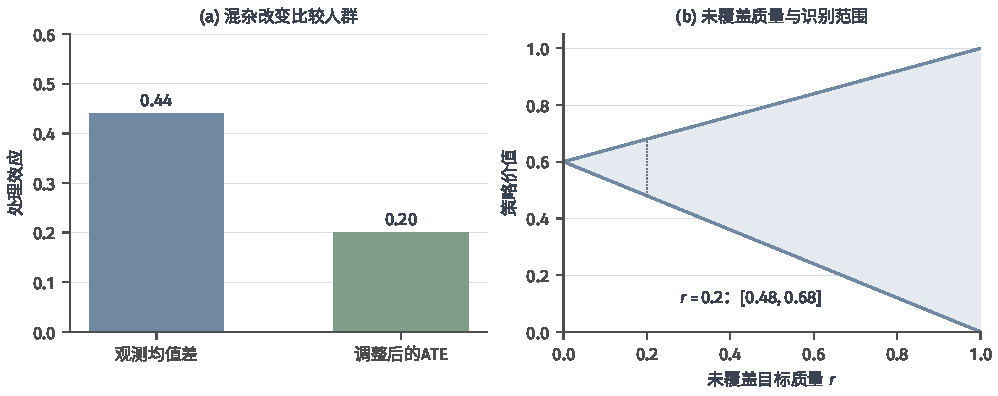
\includegraphics[width=\linewidth]{figures/02-mathematical-preliminaries-lower/01-random-variables-distributions-and-causality/matplotlib/causal-confounding-coverage/figure.pdf}
  \caption{两个独立的教学构造。左图比较风险分层例子的观测均值差\(0.44\)与调整
  效应\(0.20\)。右图按式~\eqref{eq:causal-policy-value-bounds}绘制
  \([0.6(1-r),0.6(1-r)+r]\)。阴影为总体识别范围，不是抽样置信带；
  两个面板不表示同一数据集。}
  \label{fig:causal-confounding-coverage}
\end{figure*}

这里的策略只作一次行动。第~\ref{sec:decision-dynamic-programming}节建立序贯
策略后，必须逐时检查历史覆盖、时间变化的混杂及轨迹结果定义，不能把单步权重
直接套到整条轨迹。

\subsubsection{未观测混杂下的敏感性范围}
\label{sec:causal-sensitivity-ranges}

另一种缺口不是某类记录完全没有，而是相同已观测背景下仍存在未观测选择差异。
敏感性分析不强行断言该差异为零，而是规定其允许强度，检查结论随强度怎样变化。

先用一个最小线性模型定位偏差。设变量中心化，
\[
  T=\alpha U+\varepsilon_T,\qquad
  Y=\beta T+\gamma U+\varepsilon_Y,
\]
其中\(U,\varepsilon_T,\varepsilon_Y\)两两独立、方差有限，且
\(\operatorname{Var}(T)>0\)。理想设定\(T=t\)时，固定背景的结果对\(t\)的
导数为\(\beta\)。但只将\(Y\)对自然处理\(T\)作总体线性回归，得到
\begin{equation}
  \begin{aligned}
    \beta_{\mathrm{obs}}
    &=\frac{\operatorname{Cov}(T,Y)}{\operatorname{Var}(T)}\\
    &=\beta+
      \gamma\frac{\alpha\operatorname{Var}(U)}{\operatorname{Var}(T)}.
  \end{aligned}
  \label{eq:causal-linear-confounding-bias}
\end{equation}
这里用到了
\(\operatorname{Cov}(T,Y)=\beta\operatorname{Var}(T)
+\gamma\operatorname{Cov}(T,U)\)，以及
\(\operatorname{Cov}(T,U)=\alpha\operatorname{Var}(U)\)。
共同背景同时进入处理与结果，产生了第二项。若仅支持该偏差绝对值不超过
\(\Lambda\)，则
\(\beta\in[\beta_{\mathrm{obs}}-\Lambda,\beta_{\mathrm{obs}}+\Lambda]\)。
观测可以估计\(\beta_{\mathrm{obs}}\)，却不能在没有额外信息时把
\(\alpha,\gamma,\beta\)各自分开；改变函数形式也会改变敏感性参数的含义。

异质或非线性响应不一定有一个统一斜率修正量。仍记
\(\mu_t(x)=\mathbb E[Y\mid T=t,X=x]\)和\(e(x)=\mathbb P(T=1\mid X=x)\)。
在\(0<e(x)<1\)且相关条件期望有限时，定义选择偏差函数
\[
  \begin{aligned}
    b_1(x)&=\mathbb E[Y(1)\mid T=1,X=x]
            -\mathbb E[Y(1)\mid T=0,X=x],\\
    b_0(x)&=\mathbb E[Y(0)\mid T=1,X=x]
            -\mathbb E[Y(0)\mid T=0,X=x].
  \end{aligned}
\]
条件交换性蕴含\(b_1=b_0=0\)，但反过来只得到条件均值交换性，
不能推出完整潜在结果分布相同。比如两组都均值为零，一组恒等于零，另一组等概率
取\(1,-1\)，均值相同仍保留分布差异。

一致性给出
\(\mathbb E[Y(1)\mid T=1,X=x]=\mu_1(x)\)，再由全期望
\[
  \begin{aligned}
    \mathbb E[Y(1)\mid X=x]
    &=e(x)\mu_1(x)+(1-e(x))(\mu_1(x)-b_1(x))\\
    &=\mu_1(x)-(1-e(x))b_1(x).
  \end{aligned}
\]
另一侧有
\[
  \begin{aligned}
    \mathbb E[Y(0)\mid X=x]
    &=(1-e(x))\mu_0(x)+e(x)(\mu_0(x)+b_0(x))\\
    &=\mu_0(x)+e(x)b_0(x).
  \end{aligned}
\]
相减得到
\begin{equation}
  \tau(x)=\mu_1(x)-\mu_0(x)
  -(1-e(x))b_1(x)-e(x)b_0(x).
  \label{eq:causal-selection-bias-function}
\end{equation}
若领域知识仅支持
\(|b_1(x)|\leq\Gamma_1(x)\)及\(|b_0(x)|\leq\Gamma_0(x)\)，三角不等式给出
\begin{equation}
  \begin{aligned}
    \mu_1(x)-\mu_0(x)-\Delta(x)
    &\leq\tau(x)\\
    &\leq\mu_1(x)-\mu_0(x)+\Delta(x),
  \end{aligned}
  \label{eq:causal-sensitivity-bounds}
\end{equation}
其中\(\Delta(x)=(1-e(x))\Gamma_1(x)+e(x)\Gamma_0(x)\)。
重叠在目标总体几乎处处成立、潜在结果及相应控制量可积时，再对\(X\)平均便得到
ATE范围。该范围是当前偏差约束的有效包络；若还有限定结果范围或其他联合约束，
不能未经可达性检查就宣称它为锐界。

\(\Gamma_t\)是关于未观测差异的假设，不是样本自动生成的误差条。报告应展示在多大
强度下结论变号或越过决策阈值，而不只给一个恰好保留原结论的值。
其他有根据的假设也能缩小相容类。例如个体\term{单调性}（monotonicity）
\[
  Y(1)\geq Y(0)\quad\text{几乎必然}
\]
排除所有受损个体，故ATE至少为零，可以将有效下界提高到零。
它比“平均有益”更强。若已知个体效应位于\([-\rho,\rho]\)，支持缺口中的
\([-1,1]\)可换成更窄范围；平滑外推也必须作为新增机制限制声明。

跨环境资料可以提供另一种约束。若源环境有随机试验，目标环境给出协变量分布，
并假设条件效应在两环境相同，且目标协变量分布对源环境分布绝对连续，即源环境
的零概率背景集在目标环境中也为零概率，则
\[
  \tau_{\mathrm{target}}
  =\int\tau_{\mathrm{source}}(x)\,P_{X,\mathrm{target}}(\mathrm dx).
\]
这是条件效应稳定和目标覆盖共同给出的运输关系；在离散情形，覆盖要求目标中
出现的背景在源环境也有正概率。连续情形仅有拓扑支持包含还不够，应使用上述
绝对连续条件。它们都不是看到稳定预测关联就自动成立。
共同隐藏原因、选择过程或多个机制同步变化都可能产生稳定关联。

相容类也可用于第~\ref{sec:causal-counterfactual-recourse}节的反事实、补救与公平
目标。跨世界配对不同的模型可能同样解释试验边缘，却改变行动成功概率或公平判断。
此时应传播这些模型差异，而不是仅报告选定生成模型内的模拟精度。

\subsection{有限样本下的响应估计}
\label{sec:causal-response-estimation}

即使识别式成立，条件响应、处理概率与总体权重通常仍需从样本估计。比如调整法用
\(\widehat\mu_t\)代替\(\mu_t\)，再在目标背景样本上平均：
\[
  \widehat\tau
  =\frac1n\sum_{i=1}^n
    \bigl(\widehat\mu_1(X_i)-\widehat\mu_0(X_i)\bigr).
\]
这只是识别式的一种代入估计，不自动具有无偏性或某种收敛速度。拟合误差、目标样本
的抽样误差以及重复使用同一数据引入的依赖，仍须按第~\ref{sec:rv-inference}节
的估计与数据复用规则分析。采用样本拆分或交叉拟合时，应明确哪些样本拟合、哪些
样本评价，以及相应误差条件。

逆概率法还要估计倾向概率。很小但非零的真实概率允许总体识别，却可能使估计方差
很大；截断权重可改变偏差与方差，但不能被解释为凭空补足支持。更灵活的拟合器
或交叉拟合同样不能修复交换性错误。

部分识别时，估计对象可以是识别集合的端点或其外包络。识别集合在总体分布已知时
仍可能不是单点，表达机制歧义；\term{置信区间}来自有限样本，表达总体目标、
识别集合或端点的估计误差。对端点构造置信范围，还需按所用统计方法处理两个端点
共同的覆盖要求，不能把端点估计直接当作已知真界。

实际报告应分别列出相容机制留下的范围、抽样造成的不确定性，以及积分或优化中的
数值误差。增加样本主要改善第二项，改善算法主要影响第三项；改变设计、扩大目标
行动覆盖或加入可辩护的机制限制，才可能缩小第一项。尤其在效应符号或行动阈值附近，
应同时报告对支持处理、敏感性参数及目标总体选择的依赖。

\section{因果生成结构的表示}
\label{sec:causal-generating-structure}

培训可以先改变技能，技能再改变成绩。把这些局部生成规则合起来，就能构造此前使用的整体响应映射。每条局部方程规定怎样产生一个变量，背景的联合分布规定未展开因素怎样共同变化，图则记录方程读取哪些变量。只有把这三项结合，才能计算替换处理规则后应沿哪些关系重新求值。

\subsection{局部机制的结构方程表示}
\label{sec:causal-local-structural-equations}

把模型内需要解释的变量称为内生变量，把当前模型不再解释的背景称为外生变量。
“外生”是相对于模型边界而言，并不意味着这些量在现实中没有原因，也不自动意味着
它们彼此独立。进入某个变量生成函数的其他内生变量称为它的父变量，表示该局部机制
直接读取哪些输入。

\begin{definition}[无环结构因果模型]
  \label{def:causal-structural-model}
  本章的\term{结构因果模型}（structural causal model, SCM）由内生变量
  \(\bm V=(V_1,\ldots,V_d)\)的可测状态空间、外生背景
  \(\bm U=(U_1,\ldots,U_d)\)的联合分布及可测结构函数组成：
  \begin{equation}
    V_j=f_j(\operatorname{pa}_j,U_j),
    \qquad j=1,\ldots,d.
    \label{eq:causal-scm-definition}
  \end{equation}
  其中\(\operatorname{pa}_j\)收集进入第\(j\)个函数的其他内生变量。
  \term{无环}（acyclic）要求存在节点次序\(j_1,\ldots,j_d\)，使每个函数的
  内生输入都来自次序中更早的节点。外生分量可以相关。
\end{definition}

把每个内生变量画成节点，在\(V_k\)作为输入进入\(f_j\)时画箭头\(V_k\to V_j\)，
便得到有向无环图，简称DAG。上述求值次序已足以理解无环性，不需要先学习图排序
算法。SCM的箭头具有生成语义；若箭头只用于表示联合分布的条件分解，就不能据此
判断改变输入的后果\scite{math-pearl2009causality}

例如，培训\(T\)、技能\(M\)和成绩\(Y\)可以写成
\[
  T=f_T(U_T),\qquad
  M=\alpha T+U_M,\qquad
  Y=\beta T+\gamma M+U_Y.
\]
这里的直接输入关系为\(T\to M\)、\(T\to Y\)、\(M\to Y\)。若
\(U_T,U_M,U_Y\)相关，处理选择还可能与技能或成绩背景相联系；仅画出这三条内生边
不足以表示全部共同背景。要使用独立噪声DAG的概率规则，必须另行要求这些背景独立，
或把相关性的共同来源显式放进模型。

有限维模型可以把局部函数写成\(f_{j,\bm\theta_j}\)，并用
\(\bm\theta=(\bm\theta_1,\ldots,\bm\theta_d)\)汇集参数。上例的
\(\alpha,\beta,\gamma\)是局部作用参数；一般SCM则不必属于有限维函数族。
指定关系但不知道函数，或拟合函数却没有确定它的因果语义，都仍留下结构上的未知。

\subsection{局部机制的复合与响应生成}
\label{sec:causal-mechanism-composition}

有了局部方程，定义~\ref{def:causal-response-interface}假定的自然映射就可以
实际构造。无环次序让每一步只读取已经得到的值，因此既给出计算过程，也排除了
同一背景下出现多个自然解的歧义。

\begin{theorem}[无环机制的唯一可测响应]
  \label{thm:causal-acyclic-response}
  对定义~\ref{def:causal-structural-model}中的模型，每个背景
  \(\bm u\)唯一确定一组满足所有结构方程的内生取值。
  所得自然映射\(F_M:\mathcal U\to\mathcal V\)可测。将任意指定的一组方程
  替换为常量方程后，所得映射\(F_M^a\)同样存在、唯一且可测。
  对单变量理想干预，响应\((t,\bm u)\mapsto R_M(t,\bm u)\)联合可测。
\end{theorem}
\begin{proof}
  取符合无环性的次序\(j_1,\ldots,j_d\)。第一个变量没有内生父变量，
  因而\(v_{j_1}=f_{j_1}(u_{j_1})\)唯一确定，且是\(\bm u\)的可测函数。
  假设前\(k-1\)个变量已唯一确定为可测函数。第\(k\)个方程的父变量都在其中，
  将这些函数及\(u_{j_k}\)代入可测的\(f_{j_k}\)，便得到唯一且可测的
  \(v_{j_k}\)。归纳到\(d\)，得到满足全部方程的可测向量\(F_M(\bm u)\)。
  任何另一组解在第一个坐标都必须相同；逐坐标应用同一理由，便证明唯一性。

  常量替换只删除输入，不增加逆向依赖，原次序仍可使用。被替换坐标直接取行动
  指定值，其余坐标按同样归纳求出，从而得到\(F_M^a\)。
  若把处理值\(t\)也作为输入，被替换坐标是乘积空间上的投影
  \((t,\bm u)\mapsto t\)，其余步骤仍是可测函数的复合，因此
  \(F_M^{a(t)}(\bm u)\)及其结果坐标\(R_M(t,\bm u)\)联合可测。
\end{proof}

自然分布是\((F_M)_{\#}P_{\bm U}\)，干预分布是
\((F_M^a)_{\#}P_{\bm U}\)。两个推前共用同一个背景分布，只改变生成映射。
若理想干预值恰好等于该背景下的自然处理值，那么自然解也满足替换后的全部方程；
由唯一性，两组解相同。这也证明了这种构造中的一致性，而不只是另行假定
\(Y=Y(T)\)。

若结果方程为\(Y=f_Y(T,X,U_Y)\)，且\(X\)不受处理干预影响，则
\begin{equation}
  Y(t)=f_Y(t,X,U_Y).
  \label{eq:causal-scm-potential-outcome}
\end{equation}
因此\(\mathcal L(Y(t))=\mathcal L(Y\mid\operatorname{do}(T=t))\)。
若结果还依赖处理会改变的技能\(M\)，则必须先重算\(M(t)\)，不能仍代入事实技能。
对上面的线性机制，
\[
  M(t)=\alpha t+U_M,\qquad
  Y(t)=(\beta+\gamma\alpha)t+\gamma U_M+U_Y,
\]
所以整体响应导数为\(\beta+\gamma\alpha\)，不只是局部结果方程中固定\(M\)
时的偏导数\(\beta\)。取\(\alpha=2,\beta=1,\gamma=3\)，增加一单位培训使成绩
增加\(7\)，其中直接贡献为\(1\)，经技能传递的贡献为\(6\)。
对可微的非线性机制\(M=f_M(T,U_M)\)、\(Y=f_Y(T,M,U_Y)\)，链式法则给出
\[
  \frac{\partial R_M(t,\bm u)}{\partial t}
  =
  \frac{\partial f_Y}{\partial t}
  +
  \frac{\partial f_Y}{\partial m}
  \frac{\partial f_M}{\partial t},
\]
各偏导数均在该背景的干预取值处计算。这连接了第~\ref{sec:causal-local-response}节
的整体局部变化与本节的局部方程；对它再作总体平均，仍须检查导数与积分交换条件。

在外生噪声相互独立时，还可以用局部概率核表达同一计算。记
\[
  K_j(B\mid\bm v_{\operatorname{pa}_j})
  =
  \mathbb P\bigl(f_j(\bm v_{\operatorname{pa}_j},U_j)\in B\bigr).
\]
每个核都由机制及噪声分布指定，沿无环次序复合这些核便得到联合分布。独立性保证
当前噪声不会被已经生成的变量额外筛选。若这些核具有质量函数或密度，则
\[
  p(\bm v)=\prod_{j=1}^d p(v_j\mid\operatorname{pa}_j).
\]
理想干预把处理核换成点质量，其余核保持原样，于是得到\term{截断分解}
\begin{equation}
  p(\bm v_{-T}\mid\operatorname{do}(T=t))
  =
  \prod_{j:V_j\ne T}
  p(v_j\mid\operatorname{pa}_j)\big|_{T=t}.
  \label{eq:causal-truncated-factorization}
\end{equation}
这里\(\bm v_{-T}\)表示删除处理坐标后的变量集合。公式来自机制替换，不是对
任意概率分解删除一个因子都能得到因果分布。外生噪声相关时，上述独立核复合一般
不成立；应回到完整背景的推前，或显式展开相关来源。

局部因子必须使用结构机制指定的版本。观测分布只在父变量实际出现的支持上确定
条件分布；干预若产生了未见过的父变量组合，机制可以给出答案，但资料未必能识别
该答案。随意补一个支持外的条件密度，不会把模型外推变成数据结论。

对简单结构\(X\to T\)、\(X\to Y\)、\(T\to Y\)，用独立的新随机量按
\(q(t\mid x)\)分配处理，并保持其余独立噪声机制不变，得到
\begin{equation}
  p^q(x,t,y)=p(x)q(t\mid x)p(y\mid t,x).
  \label{eq:causal-stochastic-intervention}
\end{equation}
这正是第~\ref{sec:causal-intervention-potential-outcomes}节随机干预构造的局部
表达。确定性策略用点质量核表示，不必假装它有通常的Lebesgue密度。
策略若同时改变参与人群、结果测量或其他机制，就不能只替换处理因子。
更一般的机制替换也需要保证修改后的方程有明确解；添加依赖关系时，原无环次序
可能不再适用。

循环方程说明这一边界并非形式问题。例如\(V_1=V_2+1,V_2=V_1\)无解，而
\(V_1=V_2,V_2=V_1\)有无穷多组解。反馈系统可能需要动态演化、平衡选择或额外
唯一性条件，不能直接套用本节递归证明。

\subsection{变量关系的图表示与调整条件}
\label{sec:causal-graph-adjustment}

给定结构函数以后，逐个代入就能生成干预响应。选择调整变量时却未必需要知道每个函数的具体形式：我们要判断哪些处理前背景足以阻断处理选择与结果之间的联系。图只保留局部方程的输入关系，将满足同一结构的机制放在一起考察。局部路径说明条件化为何可能消除或制造联系；全图检查再判断是否还留有其他路径，后门准则据此为前面的调整公式提供充分条件。

\subsubsection{局部因果关系与调整影响}
\label{sec:causal-local-path-patterns}

结构\(T\leftarrow X\to Y\)把\(X\)称为\(T\)与\(Y\)的
\term{共同原因}（common cause）。即使处理并不影响结果，不同\(X\)人群接受
处理的比例不同，也会使\(T,Y\)在自然记录中相关。这是混杂产生的一种方式。
第~\ref{sec:causal-adjustment-identification}节的风险分层算例正是通过在同一背景层
比较，再用同一目标权重平均，消除了由两组构成不同造成的差异。

结构\(T\to M\to Y\)中的\(M\)是\term{中介变量}（mediator）：处理对结果的
一部分影响经过它传递。若目标是总效应，固定\(M\)会阻断这部分变化；若研究同时
设定\(T=t,M=m\)的响应，则需明确这是不同的联合干预。
在线性例子中，固定中介后的处理系数为\(\beta\)，让中介随处理变化的总系数为
\(\beta+\gamma\alpha\)。这并不建立一般路径效应的识别公式，只说明两种目标不同。

结构\(T\to C\leftarrow Y\)中的\(C\)是\term{碰撞点}（collider），两条箭头
在此相遇。不以\(C\)筛选时，这条路径本身不要求两端相关；一旦给定\(C\)，却可能
引入关联。例如两个独立能力共同决定总分，入选要求总分超过阈值且两项能力可以
补偿，那么入选者中一项能力较弱的人往往需要另一项更强。若入选规则改成两项能力
分别超过各自阈值，这种负关联未必出现。关系的方向取决于选择机制，不能把选择
后的相关解释为一种能力造成另一种能力。

图~\ref{fig:causal-local-path-patterns}用双边框标记已经给定的中间变量。共同原因和中介在所画路径上都是非碰撞点，给定它们会关闭该路径；给定碰撞点则会打开原本关闭的路径，但路径活跃并不保证实际分布一定存在非零统计依赖。调整变量的作用因而取决于它在路径中的角色。较大图还可能有多条连接同一对变量的路径，关闭一个局部片段后须继续检查其他路径。
\begin{figure*}[htbp]
  \centering
  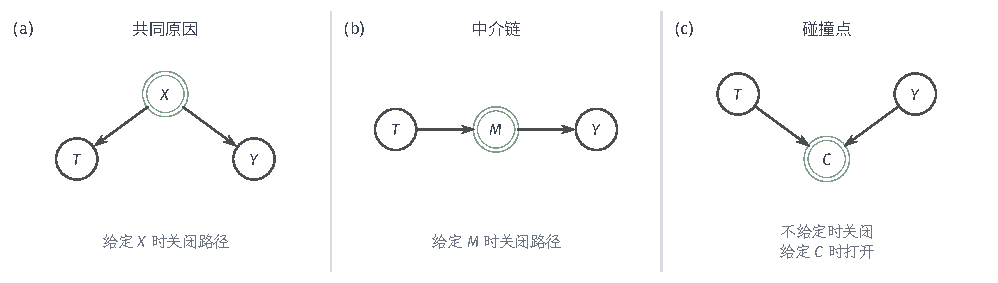
\includegraphics[width=\linewidth]{figures/02-mathematical-preliminaries-lower/01-random-variables-distributions-and-causality/tikz/causal-local-path-patterns/figure.pdf}
  \caption{共同原因、中介与碰撞点的局部路径。双边框表示节点已加入条件集。
  共同原因和中介是非碰撞点，给定后关闭这条路径；给定碰撞点则打开原本关闭的
  路径。路径打开表示图不再保证相应独立性，并不指定相关的大小或正负。}
  \label{fig:causal-local-path-patterns}
\end{figure*}

\subsubsection{全图路径分离与概率约束}
\label{sec:causal-global-path-separation}

较大图中，关闭一个局部片段仍可能留下另一条联系。设
\(\mathcal G=(V,E)\)是有向无环图，\(V\)是节点集、\(E\)是有向边集。
沿一条路径检查时，条件集中的非碰撞点会阻断路径；碰撞点自身及其后代都未被给定时，
该位置也阻断路径。只有每个位置都通过检查，整条路径才活跃。若连接两组节点的每条路径
都被阻断，就得到图分离；增加条件可能打开碰撞路径，因而分离未必保持。
这些图规则可参考\BookDefinitionRef{def:graph-theory-d-separation}{卷1《数学准备：计算、分析与几何》第9章“图的表示与计算”第9.2.4.1节“条件集合下的活跃路径”}。
本节把它们接到生成模型中的概率约束。路径指底层图中相邻且互不重复的节点序列，
有向路径才要求沿箭头前进；祖先和后代均不包括节点自身。

\begin{definition}[图分离与概率独立的记号]
  \label{def:causal-d-separation}
  对两两不交的节点集\(A,B,S\)，其中\(A,B\)非空，
  \(A\perp_{\mathcal G}B\mid S\)表示图中连接\(A,B\)的每条路径都被\(S\)
  阻断；活跃路径的碰撞与非碰撞规则沿用\BookDefinitionRef{def:graph-theory-d-separation}{卷1《数学准备：计算、分析与几何》第9章“图的表示与计算”第9.2.4.1节“条件集合下的活跃路径”}。
  若各节点承载随机变量，\(X_A\perp X_B\mid X_S\)则表示给定\(X_S\)后，
  \(X_A,X_B\)的条件联合分布分解为条件边缘分布的乘积。
  前一个记号只依赖图，后一个记号依赖概率分布；二者之间的联系需要模型假设。
\end{definition}

碰撞点是相对于某一条路径而言的，同一节点在不同路径上可以扮演不同角色。
给定其后代也可能传回选择信息，因此不能只检查碰撞点本身是否在条件集。
以同时含有
\[
  X\to M\to Y,\qquad X\to C\leftarrow Y,\qquad C\to D
\]
的图为例，\(X,Y\)之间有经过\(M\)和经过\(C\)的两条路径。四种条件集给出
不同判断：
\begin{itemize}
  \item \(S=\varnothing\)：经过\(M\)的链活跃，经过\(C\)的碰撞路径关闭，
  因而两端仍然d-连接。
  \item \(S=\{M\}\)：链被关闭，碰撞路径也仍关闭，所以
  \(X\perp_{\mathcal G}Y\mid M\)。
  \item \(S=\{M,C\}\)：链仍关闭，但给定碰撞点打开下方路径，两端重新d-连接。
  \item \(S=\{M,D\}\)：给定碰撞点的后代也打开下方路径，两端同样d-连接。
\end{itemize}
图~\ref{fig:causal-d-separation-paths}显示第二种情形。这个例子在本章即可逐路
检查；一般路径、分离与图分解的计算工具已在\BookChapterRef{chap:graph-theory}{卷1《数学准备：计算、分析与几何》第9章“图的表示与计算”}建立。
\begin{figure}[htbp]
  \centering
  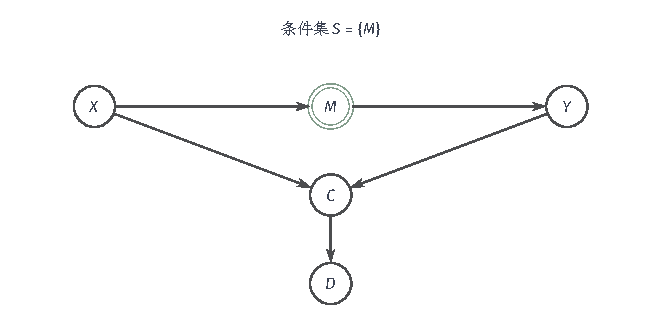
\includegraphics[width=\linewidth]{figures/02-mathematical-preliminaries-lower/01-random-variables-distributions-and-causality/tikz/causal-d-separation-paths/figure.pdf}
  \caption{多条路径下的d-分离。双边框节点\(M\)属于条件集，上方链式路径关闭；
  碰撞点\(C\)及其后代\(D\)都未给定，下方路径也关闭。若再把\(C\)或\(D\)
  加入条件集，下方路径就会打开，说明增加条件可能破坏原有的分离。}
  \label{fig:causal-d-separation-paths}
\end{figure}
\FloatBarrier

\begin{definition}[因果Markov性]
  \label{def:causal-markov-property}
  分布\(P\)相对于因果DAG \(\mathcal G\)满足\term{因果Markov性}
  （causal Markov property），是指对任意两两不交的节点集\(A,B,S\)，
  \[
    A\perp_{\mathcal G}B\mid S
    \quad\Longrightarrow\quad
    \bm V_A\perp\bm V_B\mid\bm V_S.
  \]
  其中\(\bm V_A,\bm V_B,\bm V_S\)分别收集对应节点的随机变量。
\end{definition}

左边是图规则，右边是分布性质。因果Markov性把前者的阻断结论转成条件独立；
它没有说d-连接一定产生统计依赖，也没有从观测独立直接反推箭头。它与时序过程
“给定当前状态后无须更早历史”的Markov性质使用不同对象和条件集，不能只因名称
相同就互相代入。

对DAG，这一全局表述等价于局部表述：每个变量在给定父变量后，与其非后代中除
自身和父变量外的变量条件独立。独立外生噪声的无环SCM满足这一性质。
直观上，非后代及父变量不读取当前节点的独立噪声；给定父变量后，当前变量剩下
的随机性就来自这一噪声。对局部核乘积，按逆向求值次序逐个积分掉无关后代，
每次被消去的条件核积分为一，由此保留所需的局部条件因子。分解与d-分离的
全局对应是DAG的标准结论\scite{math-pearl2009causality}
图分解与消元工具见\BookChapterRef{chap:graph-theory}{卷1《数学准备：计算、分析与几何》第9章“图的表示与计算”}；把图分离转成概率独立，
还需要这里的DAG分解或生成机制条件，不能只凭连接结构推出。
若背景相关而共同来源没有入图，不能仍对这个省略后的DAG直接宣称因果Markov性。

\subsubsection{后门条件下的调整变量选择}
\label{sec:causal-backdoor-selection}

第~\ref{sec:causal-adjustment-identification}节直接假定条件交换性，再证明调整
识别。现在可以反过来问：一张已经具有生成语义的图，能否为调整变量的选择提供
充分依据？从\(T\)到\(Y\)且第一条边指向\(T\)的路径称为
\term{后门路径}（back-door path），它从处理的自然生成来源进入比较，而非沿
处理对结果的有向作用出发。

\begin{definition}[单处理、单结果的后门准则]
  \label{def:causal-backdoor-criterion}
  设\(T,Y\)是因果DAG中的不同节点，\(Z\)与\(\{T,Y\}\)不交。若\(Z\)
  不含\(T\)的后代，且给定\(Z\)阻断所有从\(T\)到\(Y\)、第一条边指向
  \(T\)的路径，则称\(Z\)满足相对于\((T,Y)\)的
  \term{后门准则}（back-door criterion）。
\end{definition}

阻断按定义~\ref{def:causal-d-separation}判断，把碰撞点放进\(Z\)可能打开
原本关闭的路径。最基本的代表图为\(Z\to T,Z\to Y,T\to Y\)，独立噪声机制给出
\[
  p(z,t,y)=p(z)p(t\mid z)p(y\mid t,z).
\]
将处理机制替换为常量\(t\)后，
\(p(z,y\mid\operatorname{do}(T=t))=p(z)p(y\mid t,z)\)。再对背景积分，得到
\begin{equation}
  p(y\mid\operatorname{do}(T=t))
  =
  \int p(y\mid t,z)p(z)\,\mathrm dz.
  \label{eq:causal-backdoor-adjustment}
\end{equation}
离散背景用求和，一般空间用对\(P_Z\)的核积分。对结果再取期望，就回到
式~\eqref{eq:causal-g-formula}的调整表示。

一般后门准则在独立噪声无环SCM、图正确包含相关共同原因且干预保留其他机制的
条件下，给出同样的调整结论\scite{math-pearl2009causality}
阻断全部后门路径排除了自然处理选择沿这些路径携带的背景差异，非后代条件保证
用于平均的\(Z\)不先被行动改变。这些是生成结构对交换性的充分支持，而不是只由
一个观测分布满足Markov性就能推出的干预结论。即使图条件成立，要从观测资料
确定积分中的局部响应，还需要目标总体内所用处理的支持条件；图不会填补空白
协变量--处理组合。

三个局部图可以核对变量角色。在\(T\leftarrow X\to Y\)中，\(X\)关闭后门；
在\(T\to M\to Y\)中，\(M\)是后代，固定它会改变总效应目标；
在\(T\to C\leftarrow Y\)中，空条件集已经关闭碰撞路径，加入\(C\)反而打开它。
因此，处理前测量、与结果相关或能提高预测精度，都不是充分的调整标准。
后门准则是充分条件，不是识别的必要条件；它不适用时，随机设计、其他识别规则
或更具体的机制假设仍可能确定所选目标。

\section{因果生成结构的推断}
\label{sec:causal-structure-discovery}

给定图与局部机制，可以从背景逐步生成结果。反过来，仅看到结果记录时，需要辨认哪些变量进入同一局部方程，并估计方程及背景规律。关系推断改变候选图，机制推断改变给定图上的函数和噪声；两项都会影响响应。观测分布拟合只能提供相容性，唯一的方向或同背景反事实还需要额外信息。

\subsection{变量关系的推断}
\label{sec:causal-relation-inference}

从图推出分布约束与从分布反推图，是方向相反的两项任务。要用条件独立排除候选
关系，需要说明哪些独立是真正的结构阻断，哪些可能来自参数抵消。资料制度也很
重要：同分布观察、受控干预和不同环境提供的限制不一样。

\subsubsection{观测资料下的关系识别}
\label{sec:causal-observational-structure}

\begin{definition}[相对于DAG的忠实性]
  \label{def:causal-faithfulness}
  分布\(P\)相对于DAG \(\mathcal G\)满足\term{忠实性}（faithfulness），若对
  任意两两不交的节点集\(A,B,S\)，
  \[
    \bm V_A\perp\bm V_B\mid\bm V_S
    \quad\Longrightarrow\quad
    A\perp_{\mathcal G}B\mid S.
  \]
\end{definition}
忠实性要求分布中出现的条件独立能由图结构解释，不是由特殊参数抵消、确定性
约束或未处理的误差相关造成。因果Markov性给出正向蕴含，忠实性补上反向蕴含，
两者不能互相替代。

例如，设\(X,U_M,U_Y\)相互独立，
\(M=\alpha X+U_M\)，\(Y=\beta X+\gamma M+U_Y\)。
当\(\alpha,\gamma\ne0\)且\(\beta=-\gamma\alpha\)时，
\(Y=\gamma U_M+U_Y\)与\(X\)独立，但图中直接路径\(X\to Y\)及
\(X\to M\to Y\)都存在。两条贡献恰好抵消，说明无环与独立噪声并不自动保证
忠实性。接近这种抵消时，非零依赖还可能非常弱，有限样本中难以检出。

只考察三个节点且没有其他路径时，链
\(X\to Z\to Y\)、反向链\(X\leftarrow Z\leftarrow Y\)和共同原因
\(X\leftarrow Z\to Y\)都蕴含
\[
  X\perp Y\mid Z,
\]
却一般不蕴含\(X\perp Y\)。条件独立模式无法区分中间变量在传递作用还是造成
共同变化。碰撞结构\(X\to Z\leftarrow Y\)则蕴含\(X\perp Y\)，给定中间
节点后可能相关；加上忠实性，才能把这种模式差别用作反向辨识的依据。
这三种结构回用图~\ref{fig:causal-local-path-patterns}的路径规则；加入其他节点和边以后，独立判断仍须遍历全部相关路径。

\begin{definition}[Markov等价与等价类]
  \label{def:causal-markov-equivalence}
  同一节点集上的两张DAG若具有完全相同的d-分离关系，就称它们
  \term{Markov等价}（Markov equivalent）。
  与给定图Markov等价的全部DAG组成其
  \term{Markov等价类}（Markov equivalence class, MEC）。
\end{definition}

图的\term{骨架}（skeleton）是忽略箭头方向后的邻接关系。
\term{无屏蔽碰撞结构}（unshielded collider）指
\(X\to Z\leftarrow Y\)，并且两端\(X,Y\)不相邻。没有两端的直接边，才使
这个局部碰撞的差异能够通过两端的分离关系表现出来。
标准判据是：两张DAG Markov等价，当且仅当具有相同骨架和相同无屏蔽碰撞结构
\scite{pgm-structure-learning-chickering2002}

判据的必要性可以直接从全部路径证明。先说明DAG中任意两个非相邻节点都有一个
不含端点的d-分离集。选其中一个节点\(v\)，使另一个节点\(w\)不是它的后代；
无环性保证至少有这样一个选择。令条件集为\(v\)的父节点集。
任意从\(v\)到\(w\)的路径若第一条边指向\(v\)，就经过一个父节点；因两端
不相邻，该父节点是内部非碰撞点，路径被阻断。
若第一条边从\(v\)向外，路径不可能一直沿箭头到达非后代\(w\)。沿路径第一次
改变箭头方向时，出现一个碰撞点\(c\)，此前的有向前缀说明\(c\)是\(v\)的
后代。\(c\)及其任何后代都不可能成为\(v\)的父节点，否则形成有向环；
故这个碰撞点没有被条件集打开，路径仍被阻断。两类覆盖了全部路径。
相邻节点之间的单边路径则没有内部点，不可能被任何不含端点的条件集阻断。
因此，骨架不同必导致d-分离关系不同。

再考虑同一骨架上的无屏蔽三点结构\(X-Z-Y\)。两端不相邻，按上段存在分离集。
若\(Z\)不是碰撞点，任何分离集都必须包含\(Z\)，否则长度为二的这条路径
仍然活跃；若\(Z\)是碰撞点，任何分离集都不能包含\(Z\)，否则该路径被打开。
因此，中点碰撞状态不同也必然改变d-分离关系。其他路径可能增加分离要求，却
不会消除这条长度为二的路径对每个分离集施加的限制。

充分性需要控制所有较长路径，这里引用完整结构判据，不把上述必要性论证冒充
双向证明\scite{pgm-structure-learning-chickering2002}
理解等价类内部的方向变化还可借助\term{覆盖边}（covered edge）：边
\(X\to Y\)若满足
\[
  \operatorname{pa}(Y)=\operatorname{pa}(X)\cup\{X\},
\]
便是覆盖边，这里\(\operatorname{pa}(X)\)表示父节点集合。
覆盖边反转定理说明，反转这种边后仍为DAG，并保持全部d-分离关系
\scite{pgm-structure-learning-chickering2002}
从局部因子看，对给定共同父变量，这一步把
\[
  p(x\mid\operatorname{pa}(X))
  p(y\mid x,\operatorname{pa}(X))
  =
  p(y\mid\operatorname{pa}(X))
  p(x\mid y,\operatorname{pa}(X))
\]
重新分解，不改变两变量的条件联合分布。因子应取相容的条件版本；这个等式解释
分布重参数化，却没有单独证明全图等价，更没有证明两张指定图之间存在变换序列。
完整变换定理进一步保证，任意两张已知Markov等价的DAG，可以经有限次覆盖边
反转相互到达，每个中间图都保持无环且等价。这是等价类内的可达性结论，不能
代替结构判据的充分性证明\scite{pgm-structure-learning-chickering2002}

等价类可以用部分有向图表示：全部等价图都同意的方向保留箭头，其余边保持无向。
在因果Markov性、忠实性、无环和无潜在混杂等条件下，纯观测条件独立信息一般
只能识别这样的等价类。输出一条无向边并非一定表示算法未完成；它可能记录总体
观测分布本身无法决定的方向。增加同分布样本能改善独立性判断，却不会制造类内
所缺少的方向信息。

这里还隐含了变量覆盖。所有相关共同原因都已纳入可观测变量时，称满足因果充分性。
潜在共同原因能让两个可观测节点相关，却不应被硬解释成其中一个直接导致另一个。
允许潜在混杂或选择后，输出往往需要扩大到带不同端点标记的部分图，分别表示
已确定的祖先关系、可能方向和无法排除的隐藏共同原因。测量误差以及按碰撞点
选择样本也会改变独立模式，不应一律视为新增因果边。

有限样本中的关系发现还要通过检验或评分近似总体判断。以
\(H_0:V_i\perp V_j\mid\bm V_S\)为原假设，若约束型算法在未拒绝独立时
删除候选边，那么第一类错误把真实独立误判为依赖，可能保留虚假边；
第二类错误把实际依赖误判为独立，可能删除真实边。后续搜索与定向会传播错误，
评分型算法则不能直接套用这组对应。高维条件集减少每层有效样本，近忠实边界上
的弱依赖尤其难判断。结构学习的一致性必须同时说明总体的Markov与忠实条件、
检验或评分的渐近性质、候选图范围，以及搜索能否达到目标；一张确定输出图
不代表因果方向已经唯一。

\subsubsection{干预与环境变化下的方向识别}
\label{sec:causal-interventional-structure}

要打破观测方向歧义，需要增加具有不同约束的信息。理想干预切断目标变量的原
进入机制：若随机设置\(X\)后，\(Y\)的分布随设置值改变，在其余机制不变、
行动确实只作用于\(X\)的模型中，这支持\(X\)位于\(Y\)的上游。反之，没有
观察到分布改变并不自动排除作用，机制抵消、剂量范围或检验能力都可能影响判断。
对多个节点施加适当干预可缩小观测等价类，但能缩小到什么程度取决于干预覆盖。

这一证据必须按实际执行解释。干预目标未知、执行不完全，或干预同时改变测量、
选择和其他机制时，都应将这些不确定性纳入模型。不能把“鼓励参加培训”无条件
等同于“把培训处理设为指定值”，也不能把伴随整套制度改变的干预解释成单个
节点的理想替换。

不同环境也可能提供方向限制。设环境标签为\(E\)，若假定环境只改变输入\(X\)
的分布，而机制\(Y=f_Y(X,U_Y)\)及独立噪声\(U_Y\)的分布保持不变，那么
各环境在共同支持上的\(P(Y\mid X,E=e)\)应相同；反向条件分布
\(P(X\mid Y,E=e)\)却可能随输入分布变化。这里稳定性来自已声明的生成假设，
并非看到一个稳定条件分布就证明了箭头。

潜在共同原因可以在所有已观察环境中稳定，环境变化也可能太弱，未能打破错误
方向；选择规则同步变化还可能制造稳定关联。应分别说明哪些背景分布或局部
机制允许改变，哪些保持不变，环境是否直接影响结果，以及稳定性究竟是模型
假设、检验对象还是经验线索。机制知识和对隐藏混杂、弱依赖、选择过程的
敏感性分析，共同限制候选关系，不能由增加同分布样本替代。

对于反馈环、随时间改变的机制或处理定义不稳定的系统，无环静态模型本身可能
不合适，需要改用动态或循环模型并重新定义行动；方向识别不能先忽略模型边界，
再用搜索算法的精度弥补。

\subsection{局部机制的推断}
\label{sec:causal-local-mechanism-inference}

即使关系已经给定，箭头也没有给出作用大小、非线性形状和背景分布。
局部机制推断要在声明的函数族、噪声条件和观测制度内估计这些未知部分。
它可以回用第~\ref{sec:rv-inference}节的有限维参数或函数估计，但必须先明确
估计对象是否具有所需的干预含义。

例如，对已给定的父变量向量\(\bm P_j\)，假设局部方程为
\[
  V_j=\theta_{j0}+\bm\theta_j^{\mathsf T}\bm P_j+\varepsilon_j,
  \qquad
  \mathbb E[\varepsilon_j\mid\bm P_j]=0.
\]
令\(\bm Z_j=(1,\bm P_j^{\mathsf T})^{\mathsf T}\)，并令
\(\bm\vartheta_j=(\theta_{j0},\bm\theta_j^{\mathsf T})^{\mathsf T}\)。
若二阶矩有限且
\(\bm Q_j=\mathbb E[\bm Z_j\bm Z_j^{\mathsf T}]\)可逆，乘以\(\bm Z_j\)再取
期望得到
\[
  \mathbb E[\bm Z_jV_j]=\bm Q_j\bm\vartheta_j,\qquad
  \bm\vartheta_j
  =\bm Q_j^{-1}\mathbb E[\bm Z_jV_j].
\]
因此在这些条件下，局部参数可由总体矩识别。独立同分布样本中的对应矩估计为
\[
  \widehat{\bm\vartheta}_j
  =
  \left(\frac1n\sum_{i=1}^n\bm Z_{ij}\bm Z_{ij}^{\mathsf T}\right)^{-1}
  \left(\frac1n\sum_{i=1}^n\bm Z_{ij}V_{ij}\right),
\]
前提是样本矩可逆。误差、区间和正则化处理仍属于统计估计问题。真实父变量
存在确定性共线时，矩方程不能唯一确定各系数；遗漏共同背景造成条件噪声均值
非零时，拟合得到的斜率也不再自动等于局部结构参数。

在培训例子里，可以分别拟合技能方程和成绩方程，再复合为
\(\widehat\beta+\widehat\gamma\widehat\alpha\)。结果方程中的
\(\widehat\beta\)只是固定技能时的局部系数，不应独自报告为总效应。这样从
局部估计传到整体响应时，还须传播多个估计量的共同误差。

非参数情形也要区分三个层次。观测资料可以在父变量支持上估计
\(P(V_j\mid\operatorname{pa}_j)\)；把这个条件核解释为干预下保持不变的机制，
还需要正确关系、噪声及机制不变假设；再要求同一背景下不同输入怎样配对，则
需要更强的结构表示。同一组局部条件核可以由不同结构函数和背景耦合实现。
第~\ref{sec:causal-factual-counterfactual}节的两种跨世界配对已经说明，边缘
分布相同不决定已知事实后的替代结果。因此，仅拟合条件分布不能自动唯一恢复
个体响应、反事实公平或行动成功概率。

即使所有观测和干预分布都已确定，结构函数与背景仍可能有多种等价表示，因此一般SCM未必能够唯一恢复。加性独立噪声、特定函数形状和支持外的平滑性会缩小候选范围；它们应作为明确假设参与识别分析。模型在已有支持内拟合良好，只检验了这些记录上的概率预测。支持外行动的响应仍依赖外推，背景独立与机制不变也需要各自的依据。

实际可保留候选对\((\mathcal G,\{f_j\},P_{\bm U})\)，逐一生成所关心的响应，
再把这些答案送回第~\ref{sec:causal-partial-identification-sensitivity}节的
识别集合。关系不确定、局部参数或函数不确定、跨世界背景配对不确定可能贡献
不同范围；样本有限还会增加估计误差。把这些来源分别传到平均效应、策略价值
或补救约束，才不会用一个最优拟合模型掩盖其他同样相容的行动后果。

\section{本章小结}
\label{sec:causal-inference-summary}

开篇的培训问题不能只由两组成绩差回答，因为自然接受处理的人可能具有不同背景。
给定生成模型和背景分布以后，响应映射能计算主动改变处理的后果；得知某人的事实
以后，则先更新背景分布，再在同一背景下改变行动。前者改变生成规则，事实条件化
改变对背景的认识，两步不能混成从干预总体重新抽一个人。

响应比较有不同口径。同背景之差描述个体效应，对目标总体平均得到ATE，对处理前
信息分层得到CATE，比较完整边缘分布可以保留均值以外的变化，连续处理的导数则
描述局部变化。平均相同不表示无人受益或受损，干预边缘相同也不决定跨世界配对。
补救要同时声明目标、可行动变量、成本与成功保证；公平约束还须明确同背景的属性
比较及其规范含义。

能够在模型内计算，不等于能够由资料识别。明确的处理版本、一致性和无干扰使目标
与实际记录相连，随机分配或条件交换性支持响应识别，支持条件保证资料覆盖目标
会使用的协变量--行动组合。调整与逆概率表示是同一目标的不同表达。结构图建立后，
后门准则为某些调整选择提供充分依据，却不能代替目标支持，也不是全部识别方法的
必要前提。

无法点识别时，有界结果、支持缺口和敏感性约束保留所有相容答案。单调性、效应
范围、外推或跨环境稳定可以缩小模型类，但收紧来自这些新增条件。一般识别集合
不必是区间，有效包络也不自动是锐界。识别范围描述总体机制歧义，统计区间描述
有限样本误差，积分与优化还有各自的数值误差。增加同分布样本主要改善估计；
受控干预、扩大行动覆盖或增加可辩护的机制知识，才可能减少原有识别歧义。
缩小目标人群可以改善覆盖，却也改变了要回答的问题。

无环SCM把局部函数复合成唯一可测的自然及干预响应，图记录这些函数的输入关系。
因果Markov性从图推出独立约束，忠实性允许反向使用独立信息；纯观测结构发现
通常止于Markov等价类，潜在混杂、选择和测量误差还会改变候选范围。关系确定后
仍须推断局部机制，观测条件分布拟合又不自动确定同背景反事实。因此每项结论都
应列明目标、行动定义、生成假设、资料制度和剩余不确定性。

\BookChapterRef{chap:graph-theory}{卷1《数学准备：计算、分析与几何》第9章“图的表示与计算”}建立的路径、分离和结构分解为这里的图判断提供计算工具，
图本身的因果解释则来自本章的机制假设。
第~\ref{sec:decision-dynamic-programming}节将单步策略扩展到历史和序贯价值，
需要重新检查时变混杂、逐时支持与轨迹目标。
\BookChapterRef{chap:trust-fairness}{卷3《基础、理论与可信性》第13章“公平性”}与
\BookChapterRef{chap:trust-interpretability}{卷3《基础、理论与可信性》第15章“可解释性”}
分别回用反事实公平和行动补救，并补充规范要求与现实验证条件。

